\RequirePackage{fix-cm}
\documentclass[%
    twoside, openright, titlepage, numbers=noenddot,%
    cleardoublepage=plain,%
    abstractoff,
    %
    BCOR=5.5mm, paper=a4, fontsize=11pt,% A5 soft cover
    %BCOR=5.5mm, paper=21cm:29.7cm, fontsize=10pt,% 17 cm x 24 cm
    %BCOR=5mm, paper=15.59cm:23.39cm, fontsize=9pt,% Royal soft cover
    %BCOR=0mm, paper=15.24cm:22.86cm, fontsize=10pt,% US-Trade hard cover
]{scrreprt}



\usepackage{etex}
\reserveinserts{10}

% File encoding
\usepackage[utf8]{inputenc}

% Languages
\usepackage[main=english,ngerman]{babel}

% classicthesis setup
\PassOptionsToPackage{%
  %drafting,%
  %dottedtoc,%
  eulerchapternumbers,
  %listings,%
  %parts,%
  floatperchapter, pdfspacing,%
  beramono,%
  %minionprospacing,
  %subfig,%
  %eulermath,%
  a5paper,%
}{classicthesis}

% Meta
%
% Document information
%
\newcommand{\myTitle}{%
  Seamless Acceleration of numerical regular grid methods on manycore systems\xspace%
}
\newcommand{\myPlainTitle}{%
  PhD Title of the Thesis\xspace%
}

\newcommand{\myDissNumber}{?}
\newcommand{\myName}{Davide Spataro\xspace}
\newcommand{\myUni}{\protect{Universit\`a della Calabria}\xspace}
\newcommand{\myLocation}{Rende\xspace}
\newcommand{\myTime}{2017\xspace}

% DOI
\newcommand{\myDOI}{}

% Work version info
\newcommand{\worktodo}[1]{\textcolor{red}{\textbf{TODO}: #1}}
\usepackage{scrtime}
\newcommand{\workdraft}{\textcolor{gray}{Draft, \today{}---\thistime}}
% \renewcommand{\workdraft}{}
% \renewcommand{\worktodo}{}


% Hyphenation
\hyphenation{nano-elec-tro-nic}


% Finetuning
\newcounter{dummy}
\newlength{\abcd}

% Common abbreviations
\newcommand{\ie}{i.\,e.\xspace}
\newcommand{\Ie}{I.\,e.\xspace}
\newcommand{\eg}{e.\,g.\xspace}
\newcommand{\Eg}{E.\,g.\xspace}

% Handy packages
\usepackage{csquotes}  % smart quotes
\usepackage[T1]{fontenc}
\usepackage{xspace}
\usepackage{textcomp}
\usepackage{mparhack}
\usepackage{relsize}

% Biblatex
\usepackage[
backend=biber,
style=nature,
citestyle=nature 
]{biblatex}
\usepackage[
  style=nature,%
  %style=science, article-title=true,%
  natbib=true,%
  clearlang=true,%
  backend=biber,%
]{biblatex}

\ExecuteBibliographyOptions{%
  %--- Backend --- --- ---
  bibwarn=true, %
  bibencoding=auto, % (ascii, inputenc, <encoding>)
  %--- Sorting --- --- ---
  sorting=none, % Sort by name, title, year.
  % other options: 
  % nty        Sort by name, title, year.
  % nyt        Sort by name, year, title.
  % nyvt       Sort by name, year, volume, title.
  % anyt       Sort by alphabetic label, name, year, title.
  % anyvt      Sort by alphabetic label, name, year, volume, title.
  % ynt        Sort by year, name, title.
  % ydnt       Sort by year (descending), name, title.
  % none       Do not sort at all. All entries are processed in citation order.
  % debug      Sort by entry key. This is intended for debugging only.
  %
  sortcase=true,
  sortlos=los, % (bib, los) The sorting order of the list of shorthands
  sortcites=true, % do/do not sort citations according to bib	
  %--- Dates --- --- ---
  date=comp,  % (short, long, terse, comp, iso8601)
  %	origdate=
  %	eventdate=
  %	urldate=
  %	alldates=
  datezeros=true, %
  dateabbrev=true, %
  %--- General Options --- --- ---
  maxnames=3,
  minnames=1,
  maxbibnames=100, % do not abbreviate names in bibliography
  %	autocite= % (plain, inline, footnote, superscript) 
  autopunct=true,
  language=auto,
  babel=none, % (none, hyphen, other, other*)
  block=none, % (none, space, par, nbpar, ragged)
  notetype=foot+end, % (foot+end, footonly, endonly)
  hyperref=true, % (true, false, auto)
  backref=false,
  backrefstyle=three, % (none, three, two, two+, three+, all+)
  backrefsetstyle=setonly, %
  indexing=false, % 
  % options:
  % true       Enable indexing globally.
  % false      Disable indexing globally.
  % cite       Enable indexing in citations only.
  % bib        Enable indexing in the bibliography only.
  refsection=none, % (part, chapter, section, subsection)
  refsegment=none, % (none, part, chapter, section, subsection)
  abbreviate=true, % (true, false)
  defernumbers=false, % 
  punctfont=false, % 
  arxiv=abs, % (ps, pdf, format)	
  %--- Style Options --- --- ---	
  % The following options are provided by the standard styles
  isbn=false,%
  url=false,%
  doi=false,%
  eprint=false,%	
}%	

% Suppress all date fields except the year
\AtEveryBibitem{%
  \clearfield{day}%
  \clearfield{month}%
  \clearfield{endday}%
  \clearfield{endmonth}%
}

\DeclareRedundantLanguages{en,EN,English}{english}

% Use only the first page number in a given range
\DeclareFieldFormat{pages}{\mkfirstpage{#1}}

% Redefine cite command to include space before
% <http://tex.stackexchange.com/questions/11602/>
\let\origcite\cite%
\def\cite#1{\unskip~\origcite{#1}}

% Math stuff
\usepackage{amsmath}
%\usepackage{amssymb}
\usepackage{mathtools}
\usepackage{isomath}

% Figures, tables, and captions
\usepackage{tabularx}
\usepackage{ltablex}
\setlength{\extrarowheight}{3pt}
\newcommand{\tableheadline}[1]{\multicolumn{1}{c}{\spacedlowsmallcaps{#1}}}
\newcommand{\myfloatalign}{\centering}
\usepackage{floatrow}
\usepackage{caption}
\captionsetup{format=hang,font=small,labelfont={sc},margin=5pt}
\usepackage{subcaption}
\captionsetup[sub]{margin=0pt,font=small,labelfont={rm}}

% Blind text
\usepackage{blindtext}

% Hyperref
\usepackage[dvipsnames]{xcolor}
\usepackage[%
  hyperfootnotes=false,%
  pdfpagelabels,%
  % pdfa,%
]{hyperref}
\usepackage{hyperxmp}
%\pdfcompresslevel=9
%\pdfadjustspacing=1
\hypersetup{%
  %pdfstartpage=3, pdfstartview=FitV,%
  % following line: colored links (web version)
  colorlinks=true, linktocpage=true,%
  % following line: all links in black (for printing)
  %colorlinks=false, linktocpage=false, pdfborder={0 0 0},%
  breaklinks=true, pdfpagemode=UseNone, pageanchor=true, pdfpagemode=UseOutlines,%
  plainpages=false, bookmarksnumbered, bookmarksopen=true, bookmarksopenlevel=1,%
  hypertexnames=true, pdfhighlight=/O,%nesting=true,%frenchlinks,%
  pdftitle={\myPlainTitle},%
  pdfauthor={\myName},%
  pdfcopyright={Copyright (C) \myTime, \myName},%
  pdfsubject={},%
  pdfkeywords={},%
  pdflang={en},%
}

% Graphics
\usepackage{graphicx}
\usepackage{rotating}
\usepackage{tikz}
\usepackage{pgfplots}
\pgfplotsset{compat=newest}
\usetikzlibrary{shapes.geometric}

% Circled numbers
\newcommand*\circled[1]{
  \tikz[baseline=(char.base)]{
    \node[shape=circle,draw,inner sep=1pt,font=\footnotesize,%
          minimum size=0.8\baselineskip] (char) {\figureversion{lining}#1};
  }
}

% \tikzexternalize
% \tikzsetexternalprefix{externalized/}

% Autoreferences
\renewcommand*{\figureautorefname}{Figure}
\renewcommand*{\tableautorefname}{Table}
\renewcommand*{\partautorefname}{Part}
\renewcommand*{\chapterautorefname}{Chapter}
\renewcommand*{\sectionautorefname}{Section}
\renewcommand*{\subsectionautorefname}{Section}
\renewcommand*{\subsubsectionautorefname}{Section}
\providecommand{\subfigureautorefname}{\figureautorefname}%
\usepackage{cleveref}

% Acronyms
\PassOptionsToPackage{printonlyused}{acronym}
\usepackage{acronym}

% List items
\usepackage{enumitem}

% Load classicthesis style
\usepackage{scrhack}
\usepackage{classicthesis}

% Customize text width and length

\KOMAoptions{headinclude=true,footinclude=false}
\setlength{\textwidth}{10.5cm} % 9 pt font
\setlength{\textwidth}{11.6cm} % 9 pt font
\setlength{\textwidth}{15.5cm} % a4 paper 10 pt font
% text height set by golden ratio
\areaset[current]{\textwidth}{1.618034\textwidth}

% Page numbers in plain style (chapter titles)
\clearscrplain
\ofoot[\pagemark]{}
% Adjust distance to footer (default is too large)
\setlength{\footskip}{15pt}

%
% Font setup
%

% Micro-typographic extensions
%\usepackage[protrusion=true,expansion=true]{microtype}

% Use Minion Pro
%\usepackage[
%  mathlf, % lining figures
%]{MinionPro}
%\linespread{1.06}

%
% Customize colors
%
\definecolor{chapter-color}{cmyk}{1, 0.50, 0, 0.25}
\definecolor{link-color}{cmyk}{1, 0.50, 0, 0.25}
\definecolor{cite-color}{cmyk}{0, 0.7, 0.9, 0.2}

% Hyperref
\usepackage{bookmark}
\hypersetup{
  %urlcolor=webbrown, linkcolor=RoyalBlue, citecolor=webgreen, %pagecolor=RoyalBlue,%
  %urlcolor=webbrown, linkcolor=Maroon, citecolor=webgreen,%
  %urlcolor=link-color, linkcolor=link-color, citecolor=cite-color,%
  urlcolor=Black, linkcolor=Black, citecolor=Black, %pagecolor=Black,%
}

% Chapter font
\let\chapterNumber\undefined%
\newfont{\chapterNumber}{eurb10 scaled 5500}
%\newfont{\chapterNumber}{MinionPro-Regular-lf-t1 scaled 5500}

% SI units
\usepackage{siunitx}
\sisetup{
  separate-uncertainty,
  repeatunits=false,
  detect-family,
  unit-mode=text,
}
\DeclareSIUnit\au{a.u.}
\let\u=\SI%

% Product type codes
\newcommand{\productcode}[1]{\figureversion{lining}#1}

% TOC
\renewcommand{\cftpartfont}{\color{chapter-color}\normalfont}%
\renewcommand{\cftpartpagefont}{\normalfont}%

% Chapter number on inside
\titleformat{\chapter}[display]%
  {\relax}{\vspace*{-3\baselineskip}\makebox[\linewidth][r]{\color{halfgray}\chapterNumber\thechapter}}{10pt}%
  {\raggedright\spacedallcaps}[\normalsize\vspace*{.8\baselineskip}\titlerule]%

% Chapter abstract
\def\chapterabstract#1{%
  \begingroup
  \baselineskip1.3em
  \leftskip1em
  \rightskip\leftskip\itshape#1
  \par
  \endgroup
}

% Chapter quotes
% Adapted from: <http://tex.stackexchange.com/questions/53377/inspirational-quote-at-start-of-chapter>
\setkomafont{dictumtext}{\itshape\small}%
\setkomafont{dictumauthor}{\normalfont}
\renewcommand*{\dictumwidth}{0.6\textwidth}
\renewcommand*{\dictumrule}{}
\renewcommand*\dictumauthorformat[1]{--- #1}

% Subfigure labels (manual)
%\usepackage{subfigure}
%\newcommand{\subfig}[1]{#1)}
\newcommand{\subfig}[1]{(#1)}

% CV
\newcommand{\cvleft}[1]{\begin{minipage}[t]{2.5cm}\begin{flushright}#1\end{flushright}\end{minipage}\hspace{5mm}}
\newcommand{\cvright}[1]{\begin{minipage}[t]{8cm}{#1}\end{minipage}}

% Footnote without number
\newcommand\blfootnote[1]{%
  \begingroup
  \renewcommand\thefootnote{}\footnote{#1}%
  \addtocounter{footnote}{-1}%
  \endgroup
}

% Put pages on A4 w/ crop marks
%\usepackage[a4,center,cam]{crop}

% Widow and club penalties
\clubpenalty = 10000
\widowpenalty = 10000
%\displaywidowpenalty = 10000





%\usepackage{verbatim}
\usepackage{xcolor}
\definecolor{bgcolor}{rgb}{0.99,0.99,0.99}
\definecolor{light-gray}{gray}{0.95}
\usepackage{listings}

 \lstdefinelanguage[OpenCL]{C}[ANSI]{C} 
{  basicstyle=\footnotesize\ttfamily,
	breaklines=true,
	showstringspaces=false,
	numbers=none,
	backgroundcolor=\color{white},
	commentstyle=\color{red},
	keywordstyle=\color{black}\bfseries,
	keywordstyle=[1]\color{black},   % cyan or teal can also be a good choice, use \bfseries for bold
	frame=none,                     % adds a frame around the code
	%xleftmargin=\parindent,
	tabsize=2,                      % sets default tabsize to 2 spaces
	captionpos=b,
	morekeywords={__kernel,kernel,__local,local,__global,global,% 
		__constant,constant,__private,private,% 
		char2,char3,char4,char8,char16,% 
		uchar2,uchar3,uchar4,uchar8,uchar16,% 
		short2,short3,short4,short8,short16,% 
		ushort2,ushort3,ushort4,ushort8,ushort16,% 
		int2,int3,int4,int8,int16,% 
		uint2,uint3,uint4,uint8,uint16,% 
		long2,long3,long4,long8,long16,% 
		ulong2,ulong3,ulong4,ulong8,ulong16,% 
		float2,float3,float4,float8,float16,% 
		image2d_t,image3d_t,sampler_t,event_t,% 
		bool2,bool3,bool4,bool8,bool16,% 
		half2,half3,half4,half8,half16,% 
		quad,quad2,quad3,quad4,quad8,quad16,% 
		complex,imaginary},
	    morekeywords=[1]{               % if you want to add more keywords to the set
		MODELTYPE,
		__CALCL_MODEL_3D,
		MODEL_2D,
		MODEL_3D,
		CALCLcontext,
		CALCLdevice,
		CALCLkernel,
		CALCLManager,
		CALCLmem,
		CALCLModel2D,
		CALCLModel3D,
		CALCLprogram,
		CAL_CUSTOM_NEIGHBORHOOD_2D,
		CAL_CUSTOM_NEIGHBORHOOD_3D,
		CAL_FALSE,
		CALGL_DATA_TYPE_DYNAMIC,
		CALGL_DRAW_MODE_FLAT,
		CALGL_DRAW_MODE_SURFACE,
		CALGL_INFO_BAR_ORIENTATION_VERTICAL,
		CALGL_TYPE_INFO_USE_CURRENT_COLOR,
		CALGL_TYPE_INFO_USE_RED_YELLOW_SCALE,
		CALGL_TYPE_INFO_USE_NO_COLOR,
		CALGL_TYPE_INFO_COLOR_DATA,
		CALGL_TYPE_INFO_NORMAL_DATA,
		CALGL_TYPE_INFO_VERTEX_DATA,
		CALGL_TYPE_INFO_USE_CONST_VALUE,
		CALGL_TYPE_INFO_USE_DEFAULT,
		CALGL_TYPE_INFO_USE_RED_SCALE,
		CALGL_DATA_TYPE_STATIC,
		CALGLRun2D,
		CALGLRun3D,
		CALGLDrawModel2D,
		CALGLDrawModel3D,
		CAL_HEXAGONAL_NEIGHBORHOOD_2D,
		CAL_HEXAGONAL_NEIGHBORHOOD_ALT_2D,
		CAL_MOORE_NEIGHBORHOOD_2D,
		CAL_MOORE_NEIGHBORHOOD_3D,
		CAL_NO_OPT,
		CAL_OPT_ACTIVE_CELLS,
		CAL_RUN_LOOP,
		CAL_SPACE_FLAT,
		CAL_SPACE_TOROIDAL,
		CAL_TRUE,
		CAL_UPDATE_EXPLICIT,
		CAL_UPDATE_IMPLICIT,
		CAL_VON_NEUMANN_NEIGHBORHOOD_2D,
		CAL_VON_NEUMANN_NEIGHBORHOOD_3D,
		calAddActiveCell2D,
		calAddActiveCell3D,
		calAddActiveCellX2D,
		calAddActiveCellX3D,
		calAddElementaryProcess2D,
		calAddElementaryProcess3D,
		calAddSingleLayerSubstate2Db,
		calAddSingleLayerSubstate2Di,
		calAddSingleLayerSubstate2Dr,
		calAddSingleLayerSubstate3Db,
		calAddSingleLayerSubstate3Di,
		calAddSingleLayerSubstate3Dr,
		calAddSubstate2Db,
		calAddSubstate2Di,
		calAddSubstate2Dr,
		calAddSubstate3Db,
		calAddSubstate3Di,
		calAddSubstate3Dr,
		calAddActiveCell2D,
		calAddActiveCellX2D,
		calAddActiveCell3D,
		calAddActiveCellX3D,
		calApplyElementaryProcess2D,
		calApplyElementaryProcess3D,
		CALbyte,
		calclAddActiveCell2D,
		calclAddActiveCellX2D,
		calclAddElementaryProcess2D,
		calclAddElementaryProcess3D,
		calclAddReductionSum2Di,
		calclAddStopConditionFunc2D,
		calclAddStopConditionFunc3D,
		calclAddSteeringFunc2D,
		calclAddSteeringFunc3D,
		calclCreateBuffer,
		calclCreateContext,
		calclCreateManager,
		calCADef2D,
		calCADef3D,
		calclCADef2D,
		calclCADef3D,
		calclFinalizeManager,
		calclFinalize2D,
		calclFinalize3D,
		calclGet2Db,
		calclGet3Db,
		calclGet2Di,
		calclGet3Di,
		calclGet2Dr,
		calclGet3Dr,
		calclGetX2Db,
		calclGetX2Di,
		calclGetX2Dr,
		calclGetX3Db,
		calclGetX3Di,
		calclGetX3Dr,
		calclGetDevice,
		calclGetSum2Di,
		calclGlobalRow,
		calclGlobalColumn,
		calclGlobalSlice,
		calclInitializePlatforms,
		calclInitializeDevices,
		calclLoadProgram2D,
		calclLoadProgram3D,
		calclLocalRow,
		calclLocalColumn,
		calclLocalSlice,
		calclGetKernelFromProgram,
		calclGetRows,
		calclGetColumns,
		calclGetSlices,
		calclgGetByteSubstatesNum,
		calclGetIntSubstatesNum,
		calclGetRealSubstatesNum,
		calclGetCurrentByteSubstates,
		calclGetCurrentIntSubstates,
		calclGetCurrentRealSubstates,
		calclGetNextByteSubstates,
		calclGetNextIntSubstates,
		calclGetNnextRealSubstates,
		calclGetNeighborhood,
		calclGetNeighborhoodID,
		calclGetNeighborhoodSize,
		calclGetBoundaryCondition,
		calclGetPlatformAndDeviceFromStdIn,
		calclRemoveActiveCell2D,
		calclRemoveActiveCell3D,
		calclRun2D,
		calclRun3D,
		calclRunStop,
		calclSetKernelArg2D,
		calclSetKernelArg3D,
		calclThreadCheck2D,
		calclThreadCheck2D,
		calclSet2Db,
		calclSet3Db,
		calclSet2Di,
		calclSet3Di,
		calclSet2Dr,
		calclSet3Dr,
		calclActiveThreadCheck2D,
		calclActiveThreadCheck3D,
		CALDrawModel2D,
		CALDrawModel3D,
		calFinalize2D,
		calFinalize3D,
		calGet2Db,
		calGet2Di,
		calGet2Dr,
		calGet3Db,
		calGet3Di,
		calGet3Dr,
		calGetX2Db,
		calGetX2Di,
		calGetX2Dr,
		calGetX3Db,
		calGetX3Di,
		calGetX3Dr,
		calglAdd2Db,
		calglAdd3Db,
		calglAdd2Di,
		calglAdd3Di,
		calglAdd2Dr,
		calglAdd3Dr,
		calglColor2D,
		calglColor3D,
		calglDefDrawModel2D,
		calglDefDrawModel3D,
		calglDefDrawModelCL2D,
		calglDefDrawModelCL3D,
		calglDisplayDrawJBound2D,
		calglHideDrawJBound2D,
		calglInfoBar2Dr,
		calglInitViewer,
		calglMainLoop2D,
		calglMainLoop3D,
		calglRelativeInfoBar2Dr,
		calglRelativeInfoBar3Dr,
		calglRunCLDef2D,
		calglRunCLDef3D,
		calglSetDisplayStep,
		calglSetHeightOffset2D,
		calglSetHeightOffset3D,
		calInit2Db,
		calInit2Di,
		calInit2Dr,
		calInit3Db,
		calInit3Di,
		calInit3Dr,
		calInitSubstate2Db,
		calInitSubstate2Di,
		calInitSubstate2Dr,
		calInitSubstate3Db,
		calInitSubstate3Di,
		calInitSubstate3Dr,
		CALint,
		calLoadSubstate2Db,
		calLoadSubstate2Di,
		calLoadSubstate2Dr,
		calLoadSubstate3Db,
		calLoadSubstate3Di,
		calLoadSubstate3Dr,
		CALModel2D,
		CALModel3D,
		CALNeighborhood2D,
		CALNeighborhood3D,
		CALOptimization,
		CALParameterb,
		CALParameteri,
		CALParameterr,
		CALreal,
		calRemoveActiveCell2D,
		calRemoveActiveCell3D,
		CALRun2D,
		CALRun3D,
		calRun2D,
		calRun3D,
		calRunAddGlobalTransitionFunc2D,
		calRunAddGlobalTransitionFunc3D,
		calRunAddInitFunc2D,
		calRunAddInitFunc3D,
		calRunAddSteeringFunc2D,
		calRunAddSteeringFunc3D,
		calRunAddStopConditionFunc2D,
		calRunAddStopConditionFunc3D,
		calRunDef2D,
		calRunDef3D,
		calRunInitSimulation2D,
		calRunInitSimulation3D,
		calRunFinalize2D,
		calRunFinalize3D,
		calRunFinalizeSimulation2D,
		calRunFinalizeSimulation3D,
		calSaveSubstate2Db,
		calSaveSubstate2Di,
		calSaveSubstate2Dr,
		calSaveSubstate3Db,
		calSaveSubstate3Di,
		calSaveSubstate3Dr,
		calSet2Db,
		calSet2Di,
		calSet2Dr,
		calSet3Db,
		calSet3Di,
		calSet3Dr,
		calSetX2Db,
		calSetX2Di,
		calSetX2Dr,
		calSetX3Db,
		calSetX3Di,
		calSetX3Dr,
		calSetCurrent2Db,
		calSetCurrent2Di,
		calSetCurrent2Dr,
		calSetCurrent3Db,
		calSetCurrent3Di,
		calSetCurrent3Dr,
		CALSpaceBoundaryCondition,
		CALSubstate2Db,
		CALSubstate2Di,
		CALSubstate2Dr,
		CALSubstate3Db,
		CALSubstate3Di,
		CALSubstate3Dr,
		calUpdateActiveCells2D,
		calUpdateSubstate2Db,
		calUpdateSubstate2Di,
		calUpdateSubstate2Dr,
		calUpdate2D,
		calUpdate3D,
		CALUpdateMode,
	},
}% 

\lstset{language=C}
\lstset{
  basicstyle=\footnotesize\ttfamily,
  breaklines=true,
  showstringspaces=false,
  numbers=none,
  backgroundcolor=\color{white},
  commentstyle=\color{red},
  keywordstyle=\color{black}\bfseries,
  keywordstyle=[1]\color{black},   % cyan or teal can also be a good choice, use \bfseries for bold
  frame=none,                     % adds a frame around the code
  %xleftmargin=\parindent,
  tabsize=2,                      % sets default tabsize to 2 spaces
  captionpos=b,                   % sets the caption-position to bottom
  morekeywords=[1]{               % if you want to add more keywords to the set
    MODELTYPE,
    __CALCL_MODEL_3D,
    MODEL_2D,
    MODEL_3D,
    CALCLcontext,
    CALCLdevice,
    CALCLkernel,
    CALCLManager,
    CALCLmem,
    CALCLModel2D,
    CALCLModel3D,
    CALCLprogram,
    CAL_CUSTOM_NEIGHBORHOOD_2D,
    CAL_CUSTOM_NEIGHBORHOOD_3D,
    CAL_FALSE,
    CALGL_DATA_TYPE_DYNAMIC,
    CALGL_DRAW_MODE_FLAT,
    CALGL_DRAW_MODE_SURFACE,
    CALGL_INFO_BAR_ORIENTATION_VERTICAL,
    CALGL_TYPE_INFO_USE_CURRENT_COLOR,
    CALGL_TYPE_INFO_USE_RED_YELLOW_SCALE,
    CALGL_TYPE_INFO_USE_NO_COLOR,
    CALGL_TYPE_INFO_COLOR_DATA,
    CALGL_TYPE_INFO_NORMAL_DATA,
    CALGL_TYPE_INFO_VERTEX_DATA,
    CALGL_TYPE_INFO_USE_CONST_VALUE,
    CALGL_TYPE_INFO_USE_DEFAULT,
    CALGL_TYPE_INFO_USE_RED_SCALE,
    CALGL_DATA_TYPE_STATIC,
    CALGLRun2D,
    CALGLRun3D,
    CALGLDrawModel2D,
    CALGLDrawModel3D,
    CAL_HEXAGONAL_NEIGHBORHOOD_2D,
    CAL_HEXAGONAL_NEIGHBORHOOD_ALT_2D,
    CAL_MOORE_NEIGHBORHOOD_2D,
    CAL_MOORE_NEIGHBORHOOD_3D,
    CAL_NO_OPT,
    CAL_OPT_ACTIVE_CELLS,
    CAL_RUN_LOOP,
    CAL_SPACE_FLAT,
    CAL_SPACE_TOROIDAL,
    CAL_TRUE,
    CAL_UPDATE_EXPLICIT,
    CAL_UPDATE_IMPLICIT,
    CAL_VON_NEUMANN_NEIGHBORHOOD_2D,
    CAL_VON_NEUMANN_NEIGHBORHOOD_3D,
    calAddActiveCell2D,
    calAddActiveCell3D,
    calAddActiveCellX2D,
    calAddActiveCellX3D,
    calAddElementaryProcess2D,
    calAddElementaryProcess3D,
    calAddSingleLayerSubstate2Db,
    calAddSingleLayerSubstate2Di,
    calAddSingleLayerSubstate2Dr,
    calAddSingleLayerSubstate3Db,
    calAddSingleLayerSubstate3Di,
    calAddSingleLayerSubstate3Dr,
    calAddSubstate2Db,
    calAddSubstate2Di,
    calAddSubstate2Dr,
    calAddSubstate3Db,
    calAddSubstate3Di,
    calAddSubstate3Dr,
    calAddActiveCell2D,
    calAddActiveCellX2D,
    calAddActiveCell3D,
    calAddActiveCellX3D,
    calApplyElementaryProcess2D,
    calApplyElementaryProcess3D,
    CALbyte,
    calclAddActiveCell2D,
    calclAddActiveCellX2D,
    calclAddElementaryProcess2D,
    calclAddElementaryProcess3D,
    calclAddReductionSum2Di,
    calclAddStopConditionFunc2D,
    calclAddStopConditionFunc3D,
    calclAddSteeringFunc2D,
    calclAddSteeringFunc3D,
    calclCreateBuffer,
    calclCreateContext,
    calclCreateManager,
    calCADef2D,
    calCADef3D,
    calclCADef2D,
    calclCADef3D,
    calclFinalizeManager,
    calclFinalize2D,
    calclFinalize3D,
    calclGet2Db,
    calclGet3Db,
    calclGet2Di,
    calclGet3Di,
    calclGet2Dr,
    calclGet3Dr,
    calclGetX2Db,
    calclGetX2Di,
    calclGetX2Dr,
    calclGetX3Db,
    calclGetX3Di,
    calclGetX3Dr,
    calclGetDevice,
    calclGetSum2Di,
    calclGlobalRow,
    calclGlobalColumn,
    calclGlobalSlice,
    calclInitializePlatforms,
    calclInitializeDevices,
    calclLoadProgram2D,
    calclLoadProgram3D,
    calclLocalRow,
    calclLocalColumn,
    calclLocalSlice,
    calclGetKernelFromProgram,
    calclGetRows,
    calclGetColumns,
    calclGetSlices,
    calclgGetByteSubstatesNum,
    calclGetIntSubstatesNum,
    calclGetRealSubstatesNum,
    calclGetCurrentByteSubstates,
    calclGetCurrentIntSubstates,
    calclGetCurrentRealSubstates,
    calclGetNextByteSubstates,
    calclGetNextIntSubstates,
    calclGetNnextRealSubstates,
    calclGetNeighborhood,
    calclGetNeighborhoodID,
    calclGetNeighborhoodSize,
    calclGetBoundaryCondition,
    calclGetPlatformAndDeviceFromStdIn,
    calclRemoveActiveCell2D,
    calclRemoveActiveCell3D,
    calclRun2D,
    calclRun3D,
    calclRunStop,
    calclSetKernelArg2D,
    calclSetKernelArg3D,
    calclThreadCheck2D,
    calclThreadCheck2D,
    calclSet2Db,
    calclSet3Db,
    calclSet2Di,
    calclSet3Di,
    calclSet2Dr,
    calclSet3Dr,
    calclActiveThreadCheck2D,
    calclActiveThreadCheck3D,
    CALDrawModel2D,
    CALDrawModel3D,
    calFinalize2D,
    calFinalize3D,
    calGet2Db,
    calGet2Di,
    calGet2Dr,
    calGet3Db,
    calGet3Di,
    calGet3Dr,
    calGetX2Db,
    calGetX2Di,
    calGetX2Dr,
    calGetX3Db,
    calGetX3Di,
    calGetX3Dr,
    calglAdd2Db,
    calglAdd3Db,
    calglAdd2Di,
    calglAdd3Di,
    calglAdd2Dr,
    calglAdd3Dr,
    calglColor2D,
    calglColor3D,
    calglDefDrawModel2D,
    calglDefDrawModel3D,
    calglDefDrawModelCL2D,
    calglDefDrawModelCL3D,
    calglDisplayDrawJBound2D,
    calglHideDrawJBound2D,
    calglInfoBar2Dr,
    calglInitViewer,
    calglMainLoop2D,
    calglMainLoop3D,
    calglRelativeInfoBar2Dr,
    calglRelativeInfoBar3Dr,
    calglRunCLDef2D,
    calglRunCLDef3D,
    calglSetDisplayStep,
    calglSetHeightOffset2D,
    calglSetHeightOffset3D,
    calInit2Db,
    calInit2Di,
    calInit2Dr,
    calInit3Db,
    calInit3Di,
    calInit3Dr,
    calInitSubstate2Db,
    calInitSubstate2Di,
    calInitSubstate2Dr,
    calInitSubstate3Db,
    calInitSubstate3Di,
    calInitSubstate3Dr,
    CALint,
    calLoadSubstate2Db,
    calLoadSubstate2Di,
    calLoadSubstate2Dr,
    calLoadSubstate3Db,
    calLoadSubstate3Di,
    calLoadSubstate3Dr,
    CALModel2D,
    CALModel3D,
    CALNeighborhood2D,
    CALNeighborhood3D,
    CALOptimization,
    CALParameterb,
    CALParameteri,
    CALParameterr,
    CALreal,
    calRemoveActiveCell2D,
    calRemoveActiveCell3D,
    CALRun2D,
    CALRun3D,
    calRun2D,
    calRun3D,
    calRunAddGlobalTransitionFunc2D,
    calRunAddGlobalTransitionFunc3D,
    calRunAddInitFunc2D,
    calRunAddInitFunc3D,
    calRunAddSteeringFunc2D,
    calRunAddSteeringFunc3D,
    calRunAddStopConditionFunc2D,
    calRunAddStopConditionFunc3D,
    calRunDef2D,
    calRunDef3D,
    calRunInitSimulation2D,
    calRunInitSimulation3D,
    calRunFinalize2D,
    calRunFinalize3D,
    calRunFinalizeSimulation2D,
    calRunFinalizeSimulation3D,
    calSaveSubstate2Db,
    calSaveSubstate2Di,
    calSaveSubstate2Dr,
    calSaveSubstate3Db,
    calSaveSubstate3Di,
    calSaveSubstate3Dr,
    calSet2Db,
    calSet2Di,
    calSet2Dr,
    calSet3Db,
    calSet3Di,
    calSet3Dr,
    calSetX2Db,
    calSetX2Di,
    calSetX2Dr,
    calSetX3Db,
    calSetX3Di,
    calSetX3Dr,
    calSetCurrent2Db,
    calSetCurrent2Di,
    calSetCurrent2Dr,
    calSetCurrent3Db,
    calSetCurrent3Di,
    calSetCurrent3Dr,
    CALSpaceBoundaryCondition,
    CALSubstate2Db,
    CALSubstate2Di,
    CALSubstate2Dr,
    CALSubstate3Db,
    CALSubstate3Di,
    CALSubstate3Dr,
    calUpdateActiveCells2D,
    calUpdateSubstate2Db,
    calUpdateSubstate2Di,
    calUpdateSubstate2Dr,
    calUpdate2D,
    calUpdate3D,
    CALUpdateMode,
    }
}


\usepackage[final]{pdfpages}

\usepackage{verbatim}
\usepackage{xcolor}
\definecolor{bgcolor}{rgb}{0.99,0.99,0.99}
\definecolor{light-gray}{gray}{0.95}
\usepackage{listings}

 \lstdefinelanguage[OpenCL]{C}[ANSI]{C} 
{  basicstyle=\footnotesize\ttfamily,
	breaklines=true,
	showstringspaces=false,
	numbers=none,
	backgroundcolor=\color{white},
	commentstyle=\color{red},
	keywordstyle=\color{black}\bfseries,
	keywordstyle=[1]\color{black},   % cyan or teal can also be a good choice, use \bfseries for bold
	frame=none,                     % adds a frame around the code
	%xleftmargin=\parindent,
	tabsize=2,                      % sets default tabsize to 2 spaces
	captionpos=b,
	morekeywords={__kernel,kernel,__local,local,__global,global,% 
		__constant,constant,__private,private,% 
		char2,char3,char4,char8,char16,% 
		uchar2,uchar3,uchar4,uchar8,uchar16,% 
		short2,short3,short4,short8,short16,% 
		ushort2,ushort3,ushort4,ushort8,ushort16,% 
		int2,int3,int4,int8,int16,% 
		uint2,uint3,uint4,uint8,uint16,% 
		long2,long3,long4,long8,long16,% 
		ulong2,ulong3,ulong4,ulong8,ulong16,% 
		float2,float3,float4,float8,float16,% 
		image2d_t,image3d_t,sampler_t,event_t,% 
		bool2,bool3,bool4,bool8,bool16,% 
		half2,half3,half4,half8,half16,% 
		quad,quad2,quad3,quad4,quad8,quad16,% 
		complex,imaginary},
	    morekeywords=[1]{               % if you want to add more keywords to the set
		MODELTYPE,
		__CALCL_MODEL_3D,
		MODEL_2D,
		MODEL_3D,
		CALCLcontext,
		CALCLdevice,
		CALCLkernel,
		CALCLManager,
		CALCLmem,
		CALCLModel2D,
		CALCLModel3D,
		CALCLprogram,
		CAL_CUSTOM_NEIGHBORHOOD_2D,
		CAL_CUSTOM_NEIGHBORHOOD_3D,
		CAL_FALSE,
		CALGL_DATA_TYPE_DYNAMIC,
		CALGL_DRAW_MODE_FLAT,
		CALGL_DRAW_MODE_SURFACE,
		CALGL_INFO_BAR_ORIENTATION_VERTICAL,
		CALGL_TYPE_INFO_USE_CURRENT_COLOR,
		CALGL_TYPE_INFO_USE_RED_YELLOW_SCALE,
		CALGL_TYPE_INFO_USE_NO_COLOR,
		CALGL_TYPE_INFO_COLOR_DATA,
		CALGL_TYPE_INFO_NORMAL_DATA,
		CALGL_TYPE_INFO_VERTEX_DATA,
		CALGL_TYPE_INFO_USE_CONST_VALUE,
		CALGL_TYPE_INFO_USE_DEFAULT,
		CALGL_TYPE_INFO_USE_RED_SCALE,
		CALGL_DATA_TYPE_STATIC,
		CALGLRun2D,
		CALGLRun3D,
		CALGLDrawModel2D,
		CALGLDrawModel3D,
		CAL_HEXAGONAL_NEIGHBORHOOD_2D,
		CAL_HEXAGONAL_NEIGHBORHOOD_ALT_2D,
		CAL_MOORE_NEIGHBORHOOD_2D,
		CAL_MOORE_NEIGHBORHOOD_3D,
		CAL_NO_OPT,
		CAL_OPT_ACTIVE_CELLS,
		CAL_RUN_LOOP,
		CAL_SPACE_FLAT,
		CAL_SPACE_TOROIDAL,
		CAL_TRUE,
		CAL_UPDATE_EXPLICIT,
		CAL_UPDATE_IMPLICIT,
		CAL_VON_NEUMANN_NEIGHBORHOOD_2D,
		CAL_VON_NEUMANN_NEIGHBORHOOD_3D,
		calAddActiveCell2D,
		calAddActiveCell3D,
		calAddActiveCellX2D,
		calAddActiveCellX3D,
		calAddElementaryProcess2D,
		calAddElementaryProcess3D,
		calAddSingleLayerSubstate2Db,
		calAddSingleLayerSubstate2Di,
		calAddSingleLayerSubstate2Dr,
		calAddSingleLayerSubstate3Db,
		calAddSingleLayerSubstate3Di,
		calAddSingleLayerSubstate3Dr,
		calAddSubstate2Db,
		calAddSubstate2Di,
		calAddSubstate2Dr,
		calAddSubstate3Db,
		calAddSubstate3Di,
		calAddSubstate3Dr,
		calAddActiveCell2D,
		calAddActiveCellX2D,
		calAddActiveCell3D,
		calAddActiveCellX3D,
		calApplyElementaryProcess2D,
		calApplyElementaryProcess3D,
		CALbyte,
		calclAddActiveCell2D,
		calclAddActiveCellX2D,
		calclAddElementaryProcess2D,
		calclAddElementaryProcess3D,
		calclAddReductionSum2Di,
		calclAddStopConditionFunc2D,
		calclAddStopConditionFunc3D,
		calclAddSteeringFunc2D,
		calclAddSteeringFunc3D,
		calclCreateBuffer,
		calclCreateContext,
		calclCreateManager,
		calCADef2D,
		calCADef3D,
		calclCADef2D,
		calclCADef3D,
		calclFinalizeManager,
		calclFinalize2D,
		calclFinalize3D,
		calclGet2Db,
		calclGet3Db,
		calclGet2Di,
		calclGet3Di,
		calclGet2Dr,
		calclGet3Dr,
		calclGetX2Db,
		calclGetX2Di,
		calclGetX2Dr,
		calclGetX3Db,
		calclGetX3Di,
		calclGetX3Dr,
		calclGetDevice,
		calclGetSum2Di,
		calclGlobalRow,
		calclGlobalColumn,
		calclGlobalSlice,
		calclInitializePlatforms,
		calclInitializeDevices,
		calclLoadProgram2D,
		calclLoadProgram3D,
		calclLocalRow,
		calclLocalColumn,
		calclLocalSlice,
		calclGetKernelFromProgram,
		calclGetRows,
		calclGetColumns,
		calclGetSlices,
		calclgGetByteSubstatesNum,
		calclGetIntSubstatesNum,
		calclGetRealSubstatesNum,
		calclGetCurrentByteSubstates,
		calclGetCurrentIntSubstates,
		calclGetCurrentRealSubstates,
		calclGetNextByteSubstates,
		calclGetNextIntSubstates,
		calclGetNnextRealSubstates,
		calclGetNeighborhood,
		calclGetNeighborhoodID,
		calclGetNeighborhoodSize,
		calclGetBoundaryCondition,
		calclGetPlatformAndDeviceFromStdIn,
		calclRemoveActiveCell2D,
		calclRemoveActiveCell3D,
		calclRun2D,
		calclRun3D,
		calclRunStop,
		calclSetKernelArg2D,
		calclSetKernelArg3D,
		calclThreadCheck2D,
		calclThreadCheck2D,
		calclSet2Db,
		calclSet3Db,
		calclSet2Di,
		calclSet3Di,
		calclSet2Dr,
		calclSet3Dr,
		calclActiveThreadCheck2D,
		calclActiveThreadCheck3D,
		CALDrawModel2D,
		CALDrawModel3D,
		calFinalize2D,
		calFinalize3D,
		calGet2Db,
		calGet2Di,
		calGet2Dr,
		calGet3Db,
		calGet3Di,
		calGet3Dr,
		calGetX2Db,
		calGetX2Di,
		calGetX2Dr,
		calGetX3Db,
		calGetX3Di,
		calGetX3Dr,
		calglAdd2Db,
		calglAdd3Db,
		calglAdd2Di,
		calglAdd3Di,
		calglAdd2Dr,
		calglAdd3Dr,
		calglColor2D,
		calglColor3D,
		calglDefDrawModel2D,
		calglDefDrawModel3D,
		calglDefDrawModelCL2D,
		calglDefDrawModelCL3D,
		calglDisplayDrawJBound2D,
		calglHideDrawJBound2D,
		calglInfoBar2Dr,
		calglInitViewer,
		calglMainLoop2D,
		calglMainLoop3D,
		calglRelativeInfoBar2Dr,
		calglRelativeInfoBar3Dr,
		calglRunCLDef2D,
		calglRunCLDef3D,
		calglSetDisplayStep,
		calglSetHeightOffset2D,
		calglSetHeightOffset3D,
		calInit2Db,
		calInit2Di,
		calInit2Dr,
		calInit3Db,
		calInit3Di,
		calInit3Dr,
		calInitSubstate2Db,
		calInitSubstate2Di,
		calInitSubstate2Dr,
		calInitSubstate3Db,
		calInitSubstate3Di,
		calInitSubstate3Dr,
		CALint,
		calLoadSubstate2Db,
		calLoadSubstate2Di,
		calLoadSubstate2Dr,
		calLoadSubstate3Db,
		calLoadSubstate3Di,
		calLoadSubstate3Dr,
		CALModel2D,
		CALModel3D,
		CALNeighborhood2D,
		CALNeighborhood3D,
		CALOptimization,
		CALParameterb,
		CALParameteri,
		CALParameterr,
		CALreal,
		calRemoveActiveCell2D,
		calRemoveActiveCell3D,
		CALRun2D,
		CALRun3D,
		calRun2D,
		calRun3D,
		calRunAddGlobalTransitionFunc2D,
		calRunAddGlobalTransitionFunc3D,
		calRunAddInitFunc2D,
		calRunAddInitFunc3D,
		calRunAddSteeringFunc2D,
		calRunAddSteeringFunc3D,
		calRunAddStopConditionFunc2D,
		calRunAddStopConditionFunc3D,
		calRunDef2D,
		calRunDef3D,
		calRunInitSimulation2D,
		calRunInitSimulation3D,
		calRunFinalize2D,
		calRunFinalize3D,
		calRunFinalizeSimulation2D,
		calRunFinalizeSimulation3D,
		calSaveSubstate2Db,
		calSaveSubstate2Di,
		calSaveSubstate2Dr,
		calSaveSubstate3Db,
		calSaveSubstate3Di,
		calSaveSubstate3Dr,
		calSet2Db,
		calSet2Di,
		calSet2Dr,
		calSet3Db,
		calSet3Di,
		calSet3Dr,
		calSetX2Db,
		calSetX2Di,
		calSetX2Dr,
		calSetX3Db,
		calSetX3Di,
		calSetX3Dr,
		calSetCurrent2Db,
		calSetCurrent2Di,
		calSetCurrent2Dr,
		calSetCurrent3Db,
		calSetCurrent3Di,
		calSetCurrent3Dr,
		CALSpaceBoundaryCondition,
		CALSubstate2Db,
		CALSubstate2Di,
		CALSubstate2Dr,
		CALSubstate3Db,
		CALSubstate3Di,
		CALSubstate3Dr,
		calUpdateActiveCells2D,
		calUpdateSubstate2Db,
		calUpdateSubstate2Di,
		calUpdateSubstate2Dr,
		calUpdate2D,
		calUpdate3D,
		CALUpdateMode,
	},
}% 

\lstset{language=C}
\lstset{
  basicstyle=\footnotesize\ttfamily,
  breaklines=true,
  showstringspaces=false,
  numbers=none,
  backgroundcolor=\color{white},
  commentstyle=\color{red},
  keywordstyle=\color{black}\bfseries,
  keywordstyle=[1]\color{black},   % cyan or teal can also be a good choice, use \bfseries for bold
  frame=none,                     % adds a frame around the code
  %xleftmargin=\parindent,
  tabsize=2,                      % sets default tabsize to 2 spaces
  captionpos=b,                   % sets the caption-position to bottom
  morekeywords=[1]{               % if you want to add more keywords to the set
    MODELTYPE,
    __CALCL_MODEL_3D,
    MODEL_2D,
    MODEL_3D,
    CALCLcontext,
    CALCLdevice,
    CALCLkernel,
    CALCLManager,
    CALCLmem,
    CALCLModel2D,
    CALCLModel3D,
    CALCLprogram,
    CAL_CUSTOM_NEIGHBORHOOD_2D,
    CAL_CUSTOM_NEIGHBORHOOD_3D,
    CAL_FALSE,
    CALGL_DATA_TYPE_DYNAMIC,
    CALGL_DRAW_MODE_FLAT,
    CALGL_DRAW_MODE_SURFACE,
    CALGL_INFO_BAR_ORIENTATION_VERTICAL,
    CALGL_TYPE_INFO_USE_CURRENT_COLOR,
    CALGL_TYPE_INFO_USE_RED_YELLOW_SCALE,
    CALGL_TYPE_INFO_USE_NO_COLOR,
    CALGL_TYPE_INFO_COLOR_DATA,
    CALGL_TYPE_INFO_NORMAL_DATA,
    CALGL_TYPE_INFO_VERTEX_DATA,
    CALGL_TYPE_INFO_USE_CONST_VALUE,
    CALGL_TYPE_INFO_USE_DEFAULT,
    CALGL_TYPE_INFO_USE_RED_SCALE,
    CALGL_DATA_TYPE_STATIC,
    CALGLRun2D,
    CALGLRun3D,
    CALGLDrawModel2D,
    CALGLDrawModel3D,
    CAL_HEXAGONAL_NEIGHBORHOOD_2D,
    CAL_HEXAGONAL_NEIGHBORHOOD_ALT_2D,
    CAL_MOORE_NEIGHBORHOOD_2D,
    CAL_MOORE_NEIGHBORHOOD_3D,
    CAL_NO_OPT,
    CAL_OPT_ACTIVE_CELLS,
    CAL_RUN_LOOP,
    CAL_SPACE_FLAT,
    CAL_SPACE_TOROIDAL,
    CAL_TRUE,
    CAL_UPDATE_EXPLICIT,
    CAL_UPDATE_IMPLICIT,
    CAL_VON_NEUMANN_NEIGHBORHOOD_2D,
    CAL_VON_NEUMANN_NEIGHBORHOOD_3D,
    calAddActiveCell2D,
    calAddActiveCell3D,
    calAddActiveCellX2D,
    calAddActiveCellX3D,
    calAddElementaryProcess2D,
    calAddElementaryProcess3D,
    calAddSingleLayerSubstate2Db,
    calAddSingleLayerSubstate2Di,
    calAddSingleLayerSubstate2Dr,
    calAddSingleLayerSubstate3Db,
    calAddSingleLayerSubstate3Di,
    calAddSingleLayerSubstate3Dr,
    calAddSubstate2Db,
    calAddSubstate2Di,
    calAddSubstate2Dr,
    calAddSubstate3Db,
    calAddSubstate3Di,
    calAddSubstate3Dr,
    calAddActiveCell2D,
    calAddActiveCellX2D,
    calAddActiveCell3D,
    calAddActiveCellX3D,
    calApplyElementaryProcess2D,
    calApplyElementaryProcess3D,
    CALbyte,
    calclAddActiveCell2D,
    calclAddActiveCellX2D,
    calclAddElementaryProcess2D,
    calclAddElementaryProcess3D,
    calclAddReductionSum2Di,
    calclAddStopConditionFunc2D,
    calclAddStopConditionFunc3D,
    calclAddSteeringFunc2D,
    calclAddSteeringFunc3D,
    calclCreateBuffer,
    calclCreateContext,
    calclCreateManager,
    calCADef2D,
    calCADef3D,
    calclCADef2D,
    calclCADef3D,
    calclFinalizeManager,
    calclFinalize2D,
    calclFinalize3D,
    calclGet2Db,
    calclGet3Db,
    calclGet2Di,
    calclGet3Di,
    calclGet2Dr,
    calclGet3Dr,
    calclGetX2Db,
    calclGetX2Di,
    calclGetX2Dr,
    calclGetX3Db,
    calclGetX3Di,
    calclGetX3Dr,
    calclGetDevice,
    calclGetSum2Di,
    calclGlobalRow,
    calclGlobalColumn,
    calclGlobalSlice,
    calclInitializePlatforms,
    calclInitializeDevices,
    calclLoadProgram2D,
    calclLoadProgram3D,
    calclLocalRow,
    calclLocalColumn,
    calclLocalSlice,
    calclGetKernelFromProgram,
    calclGetRows,
    calclGetColumns,
    calclGetSlices,
    calclgGetByteSubstatesNum,
    calclGetIntSubstatesNum,
    calclGetRealSubstatesNum,
    calclGetCurrentByteSubstates,
    calclGetCurrentIntSubstates,
    calclGetCurrentRealSubstates,
    calclGetNextByteSubstates,
    calclGetNextIntSubstates,
    calclGetNnextRealSubstates,
    calclGetNeighborhood,
    calclGetNeighborhoodID,
    calclGetNeighborhoodSize,
    calclGetBoundaryCondition,
    calclGetPlatformAndDeviceFromStdIn,
    calclRemoveActiveCell2D,
    calclRemoveActiveCell3D,
    calclRun2D,
    calclRun3D,
    calclRunStop,
    calclSetKernelArg2D,
    calclSetKernelArg3D,
    calclThreadCheck2D,
    calclThreadCheck2D,
    calclSet2Db,
    calclSet3Db,
    calclSet2Di,
    calclSet3Di,
    calclSet2Dr,
    calclSet3Dr,
    calclActiveThreadCheck2D,
    calclActiveThreadCheck3D,
    CALDrawModel2D,
    CALDrawModel3D,
    calFinalize2D,
    calFinalize3D,
    calGet2Db,
    calGet2Di,
    calGet2Dr,
    calGet3Db,
    calGet3Di,
    calGet3Dr,
    calGetX2Db,
    calGetX2Di,
    calGetX2Dr,
    calGetX3Db,
    calGetX3Di,
    calGetX3Dr,
    calglAdd2Db,
    calglAdd3Db,
    calglAdd2Di,
    calglAdd3Di,
    calglAdd2Dr,
    calglAdd3Dr,
    calglColor2D,
    calglColor3D,
    calglDefDrawModel2D,
    calglDefDrawModel3D,
    calglDefDrawModelCL2D,
    calglDefDrawModelCL3D,
    calglDisplayDrawJBound2D,
    calglHideDrawJBound2D,
    calglInfoBar2Dr,
    calglInitViewer,
    calglMainLoop2D,
    calglMainLoop3D,
    calglRelativeInfoBar2Dr,
    calglRelativeInfoBar3Dr,
    calglRunCLDef2D,
    calglRunCLDef3D,
    calglSetDisplayStep,
    calglSetHeightOffset2D,
    calglSetHeightOffset3D,
    calInit2Db,
    calInit2Di,
    calInit2Dr,
    calInit3Db,
    calInit3Di,
    calInit3Dr,
    calInitSubstate2Db,
    calInitSubstate2Di,
    calInitSubstate2Dr,
    calInitSubstate3Db,
    calInitSubstate3Di,
    calInitSubstate3Dr,
    CALint,
    calLoadSubstate2Db,
    calLoadSubstate2Di,
    calLoadSubstate2Dr,
    calLoadSubstate3Db,
    calLoadSubstate3Di,
    calLoadSubstate3Dr,
    CALModel2D,
    CALModel3D,
    CALNeighborhood2D,
    CALNeighborhood3D,
    CALOptimization,
    CALParameterb,
    CALParameteri,
    CALParameterr,
    CALreal,
    calRemoveActiveCell2D,
    calRemoveActiveCell3D,
    CALRun2D,
    CALRun3D,
    calRun2D,
    calRun3D,
    calRunAddGlobalTransitionFunc2D,
    calRunAddGlobalTransitionFunc3D,
    calRunAddInitFunc2D,
    calRunAddInitFunc3D,
    calRunAddSteeringFunc2D,
    calRunAddSteeringFunc3D,
    calRunAddStopConditionFunc2D,
    calRunAddStopConditionFunc3D,
    calRunDef2D,
    calRunDef3D,
    calRunInitSimulation2D,
    calRunInitSimulation3D,
    calRunFinalize2D,
    calRunFinalize3D,
    calRunFinalizeSimulation2D,
    calRunFinalizeSimulation3D,
    calSaveSubstate2Db,
    calSaveSubstate2Di,
    calSaveSubstate2Dr,
    calSaveSubstate3Db,
    calSaveSubstate3Di,
    calSaveSubstate3Dr,
    calSet2Db,
    calSet2Di,
    calSet2Dr,
    calSet3Db,
    calSet3Di,
    calSet3Dr,
    calSetX2Db,
    calSetX2Di,
    calSetX2Dr,
    calSetX3Db,
    calSetX3Di,
    calSetX3Dr,
    calSetCurrent2Db,
    calSetCurrent2Di,
    calSetCurrent2Dr,
    calSetCurrent3Db,
    calSetCurrent3Di,
    calSetCurrent3Dr,
    CALSpaceBoundaryCondition,
    CALSubstate2Db,
    CALSubstate2Di,
    CALSubstate2Dr,
    CALSubstate3Db,
    CALSubstate3Di,
    CALSubstate3Dr,
    calUpdateActiveCells2D,
    calUpdateSubstate2Db,
    calUpdateSubstate2Di,
    calUpdateSubstate2Dr,
    calUpdate2D,
    calUpdate3D,
    CALUpdateMode,
    }
}


\usepackage{tikz}
\usetikzlibrary{positioning,chains,fit,shapes,calc, matrix,arrows, decorations.markings}
% for double arrows a la chef
% adapt line thickness and line width, if needed
\tikzstyle{vecArrow} = [thick, decoration={markings,mark=at position
	1 with {\arrow[semithick]{open triangle 60}}},
double distance=1.4pt, shorten >= 5.5pt,
preaction = {decorate},
postaction = {draw,line width=1.4pt, white,shorten >= 4.5pt}]
\tikzstyle{innerWhite} = [semithick, white,line width=1.4pt, shorten >= 4.5pt]


\usetikzlibrary{positioning}
%inparaenum
%\usepackage{paralist}
%\usepackage{wrapfig,booktabs}
%\usepackage{float}
\usepackage{siunitx}
\usepackage[linesnumbered,ruled,vlined]{algorithm2e}
\usepackage{dirtytalk}
\usepackage[framemethod=tikz]{mdframed}


\usepackage{tabularx,colortbl}
\usepackage{adjustbox}
\usepackage{nomencl}
\usepackage{physics}
\usepackage{subcaption}
\makenomenclature

\usepackage{booktabs}
\newcolumntype{L}{>{$}l<{$}} % math-mode version of "l" column type
\newcolumntype{C}{>{$}c<{$}} % math-mode version of "l" column type

\usepackage{multirow}
%\newcommand{\ra}[1]{\renewcommand{\arraystretch}{#1}}


\newcommand{\dimensional}[1] {
	\left[\vb{#1}\right]
}
%lettrine color
\renewcommand{\LettrineFontHook}{\color[gray]{0.45}}

% Bibliography
\addbibresource{main.bib}

%\addbibresource{ownpubs.bib}
%\addbibresource{bibliography.bib}
%\addbibresource{misc.bib}
\usepackage{amssymb,graphicx}
\renewcommand{\floatpagefraction}{.72}
\usepackage{wrapfig}
\usepackage{lettrine}
\newcommand{\eqname}[1]{\tag*{#1}}% Tag equation with name
\usepackage{paralist}
\begin{document}
\frenchspacing
\raggedbottom%
\selectlanguage{english}
\pagenumbering{roman}
\pagestyle{scrplain}

%
% Cover
%
% Uncomment and adapt these line\dfrac{s}{den} if you want to include a cover PDF.
%
%\includepdf[pages={1,{}}]{cover/crop/cover_front.pdf}
\cleardoublepage\setcounter{page}{1}

%
% Frontmatter
%

%*******************************************************
% Little Dirty Titlepage
%*******************************************************
\thispagestyle{empty}
%*******************************************************
\begin{center}
    \spacedlowsmallcaps{\myName} \\ \medskip                        

    \begingroup
        \color{chapter-color}\spacedallcaps{\myTitle}
    \endgroup
\end{center}        

%*******************************************************
% Titlepage
%*******************************************************
\begin{titlepage}
	% if you want the titlepage to be centered, uncomment and fine-tune the line below (KOMA classes environment)
	%\begin{addmargin}[-1cm]{-3cm}
    \begin{center}
        \large
        %\begingroup
         %   \spacedlowsmallcaps{Diss. ETH No. \myDissNumber}
        %\endgroup

        \hfill

        \vfill

        \begingroup
            \spacedallcaps{\myTitle}
            %\spacedallcaps{\myTitleLineOne}\\
            %\spacedallcaps{\myTitleLineTwo}\\
            %\spacedallcaps{\myTitleLineThree}
        \endgroup

        \vfill

        \begingroup
            A dissertation submitted to attain the degree of\\
            \vspace{0.5em}
            \spacedlowsmallcaps{Doctor of Philosophy}
            of
            \spacedlowsmallcaps{Universit\`a della Calabria} \\
            (Ph.D.\ Universit\`a della Calabria)
        \endgroup

        \vfill

        \begingroup
            presented by\\
            \vspace{0.5em}
            \spacedlowsmallcaps{\myName}\\
           % Dipl., Eidgenössisches Polytechnikum \\
            \vspace{0.5em}
            born on 14 February 1990\\
        \endgroup

        \vfill

 \begingroup
      Supervisors\\
    \vspace{0.5em}
     Prof.\ William Spataro\\
     Prof.\ Donato D'Ambrosio
 \endgroup
       % \begingroup
      %      accepted on the recommendation of\\
        %    \vspace{0.5em}
        %    Prof.\ Dr.\ A. Kleiner, examiner\\
       %     Prof.\ Dr.\ H. Burkhardt, co-examiner
       % \endgroup

        \vfill

        \myTime%

        \vfill
    \end{center}
  %\end{addmargin}
\end{titlepage}

\thispagestyle{empty}

\hfill

\vfill

\noindent\myName: \textit{\myTitle,} %\mySubtitle, %\myDegree, 
\textcopyright\ \myTime

\bigskip

\noindent\spacedlowsmallcaps{DOI}: \myDOI

%\bigskip
%
%\noindent\spacedlowsmallcaps{Supervisors}: \\
%\myProf \\
%\myOtherProf \\ 
%\mySupervisor
%
%\medskip
%
%\noindent\spacedlowsmallcaps{Location}: \\
%\myLocation
%
%\medskip
%
%\noindent\spacedlowsmallcaps{Time Frame}: \\
%\myTime

%\cleardoublepage%*******************************************************
% Dedication
%*******************************************************
\thispagestyle{empty}
%\phantomsection
\refstepcounter{dummy}
%\pdfbookmark[1]{Dedication}{Dedication}

\vspace*{3cm}

\begin{center}
    Alla Mia Famiglia.
\end{center}

\medskip

%\cleardoublepage%*******************************************************
% Abstract
%*******************************************************
%\renewcommand{\abstractname}{Abstract}
\pdfbookmark[1]{Abstract}{Abstract}
\begingroup
\let\clearpage\relax
\let\cleardoublepage\relax
\let\cleardoublepage\relax

\chapter*{Abstract}

Over the last two decades, a lot has changed regarding the way modern scientific applications are designed, written and executed, especially in the field of data-analytics, scientific computing and visualization. Dedicated computing machines are nowadays large, powerful agglomerates of hundreds or thousands of multi-core computing nodes interconnected via  network each coupled with multiple accelerators. Those kinds of parallel machines are very complex and their efficient programming is hard, bug-prone and time-consuming. 
In the field of scientific computing, and of modeling and simulation especially, parallel machines are used to obtain approximate numerical solutions to differential equations
for which the classical approach often fails to solve them analytically making a numerical computer-based approach absolutely necessary.
An approximate numerical solution of a partial differential equation can be obtained by applying a number of methods, as the finite element or finite difference method which yields approximate values of the unknowns at a discrete number of points over the domain.
When large domains are considered, big parallel machines are required in order to process the resulting huge amount of mesh nodes. Parallel programming is notoriously complex, often requiring great programming efforts in order to obtain efficient solvers targeting large computing cluster. This is especially true since heterogeneous hardware and GPGPU has become mainstream.
The main thrust of this work is the creation of a programming abstraction and a runtime library for seamless implementation of numerical methods on regular grids targeting different computer architecture: from commodity single-core laptops to large clusters of heterogeneous accelerators. A framework, \texttt{OpenCAL} had been developed, which exposes a domain specific language for the definition of a large class of numerical models and their subsequent deployment on the targeted machines. Architecture programming details are abstracted from the programmer that with little or no intervention at all can obtain a \textit{serial, multi-core, single-GPU, multi-GPUs and cluster of GPUs} \texttt{OpenCAL} application. 
Results show that the framework is effective in reducing programmer effort in producing efficient parallel numerical solvers.


\endgroup

\cleardoublepage%

\begingroup
\let\clearpage\relax
\let\cleardoublepage\relax
\let\cleardoublepage\relax

%\begin{otherlanguage}{nitalian}
\pdfbookmark[1]{Sommario}{Sommario}
\chapter*{Sommario}


Over the last two decades, a lot has changed regarding the way modern scientific applications are designed, written and executed, especially in the field of data-analytics, scientific computing and visualization. Dedicated computing machines are nowadays large, powerful agglomerates of hundreds or thousands of multi-core computing nodes interconnected via  network each coupled with multiple accelerators. Those kinds of parallel machines are very complex and their efficient programming is hard, bug-prone and time-consuming. 
In the field of scientific computing, and of modeling and simulation especially, parallel machines are used to obtain approximate numerical solutions to differential equations
for which the classical approach often fails to solve them analytically making a numerical computer-based approach absolutely necessary.
An approximate numerical solution of a partial differential equation can be obtained by applying a number of methods, as the finite element or finite difference method which yields approximate values of the unknowns at a discrete number of points over the domain.
When large domains are considered, big parallel machines are required in order to process the resulting huge amount of mesh nodes. Parallel programming is notoriously complex, often requiring great programming efforts in order to obtain efficient solvers targeting large computing cluster. This is especially true since heterogeneous hardware and GPGPU has become mainstream.
The main thrust of this work is the creation of a programming abstraction and a runtime library for seamless implementation of numerical methods on regular grids targeting different computer architecture: from commodity single-core laptops to large clusters of heterogeneous accelerators. A framework, \texttt{OpenCAL} had been developed, which exposes a domain specific language for the definition of a large class of numerical models and their subsequent deployment on the targeted machines. Architecture programming details are abstracted from the programmer that with little or no intervention at all can obtain a \textit{serial, multi-core, single-GPU, multi-GPUs and cluster of GPUs} \texttt{OpenCAL} application. 
Results show that the framework is effective in reducing programmer effort in producing efficient parallel numerical solvers.


%\end{otherlanguage}

\endgroup

\vfill
%\cleardoublepage%*******************************************************
% Acknowledgments
%*******************************************************
\pdfbookmark[1]{Acknowledgements}{acknowledgements}

\bigskip

\begingroup
\let\clearpage\relax
\let\cleardoublepage\relax
\let\cleardoublepage\relax
\chapter*{Acknowledgements}

\def\thanks#1{%
\begingroup
\leftskip1em
\noindent #1
\par
\endgroup
}

\section*{Acknowledgments}
I would like to thank my supervisors \textbf{William Spataro} and \textbf{Donato D'Ambrosio} for their invaluable support and encouragement and for believing in me from the beginning of this  Ph.D. I really wish every Ph.D. student in the world have supervisors like them. 
I would also like to thank \textbf{Alessio De Rango} and \textbf{Paola Arcuri} who were of invaluable help and for being such a great study partners.

I would like to thank \texttt{NVIDIA} corporation for providing the \textit{GTX980 GPU}
and \textit{Tesla K40} coprocessor I have used to carry out my research.

I would also like to thank also to \textbf{Prof. Filippo Melascina} from the Institute of BioEngineering of the University of Edinburgh (UK) who kindly gave access to the microscopy equipment and to \textbf{Alice Mari} who was of great help in providing the experimental raw data and subsequently in analyzing the results obtained in chapter \ref{ch:bacteria}.

I would also like to thank \textbf{Prof. Jin Ooi} for giving the opportunity to being a research visiting student at the University of Edinburgh for 10 months (October 2016 - July 2017) working on the VELaSSCO EU project and, \textbf{Prof. Gihan R. Mudalige}, who supervised me during a three months visiting period (June- September 2017) at University of Warwick, while I was investigating a novel MPI implementation of an algorithm for solving tridiagonal linear systems within the context of the OPS framework.

I would also like to thanks all the people who I have met during these years and from which I have learned and, with whom I have enjoyed together, so many things.

A special thank to all friends, especially to \textbf{Vincenzo Curti}  with whom I have shared so many important moments during this journey.

\endgroup

\pagestyle{headings}
\cleardoublepage%*******************************************************
% Table of Contents
%*******************************************************
%\phantomsection
\refstepcounter{dummy}
\pdfbookmark[1]{\contentsname}{tableofcontents}
\setcounter{tocdepth}{2} % <-- 2 includes up to subsections in the ToC
\setcounter{secnumdepth}{3} % <-- 3 numbers up to subsubsections
\manualmark%
\markboth{\spacedlowsmallcaps{\contentsname}}{\spacedlowsmallcaps{\contentsname}}
\tableofcontents
\automark[section]{chapter}
\renewcommand{\chaptermark}[1]{\markboth{\spacedlowsmallcaps{#1}}{\spacedlowsmallcaps{#1}}}
\renewcommand{\sectionmark}[1]{\markright{\thesection\enspace\spacedlowsmallcaps{#1}}}
%*******************************************************
% List of Figures and of the Tables
%*******************************************************
\clearpage

\begingroup
    \let\clearpage\relax
    \let\cleardoublepage\relax
    \let\cleardoublepage\relax
    %*******************************************************
    % List of Figures
    %*******************************************************
    \phantomsection
     \refstepcounter{dummy}
    \addcontentsline{toc}{chapter}{\listfigurename}
     \pdfbookmark[1]{\listfigurename}{lof}
\begin{scriptsize}
     \listoffigures
\end{scriptsize}


\normalsize
    % \vspace{8ex}

    %*******************************************************
    % List of Tables
    %*******************************************************
    \phantomsection
     \refstepcounter{dummy}
    \addcontentsline{toc}{chapter}{\listtablename}
     \pdfbookmark[1]{\listtablename}{lot}
\begin{scriptsize}
    \listoftables
   
   \lstlistoflistings
 \end{scriptsize}
     \vspace{8ex}
     \newpage

    %*******************************************************
    % List of Listings
    %*******************************************************
    % \phantomsection
    %\refstepcounter{dummy}
   % \addcontentsline{toc}{chapter}{\lstlistlistingname}
   % \pdfbookmark[1]{\lstlistlistingname}{lol}
    %\lstlistoflistings%

    \vspace{8ex}

%    % Notation
%    \refstepcounter{dummy}
%    \pdfbookmark[1]{Notation}{notation}
%    \markboth{\spacedlowsmallcaps{Notation}}{\spacedlowsmallcaps{Notation}}
%    \chapter*{Notation}
%
%    \section*{Frequently used symbols}%
%    \vskip -2em
%    \begin{tabularx}{\textwidth}{lX}
%      %\toprule%
%      %\tableheadline{Symbol} & \tableheadline{Meaning} \\
%      %\midrule%
%      $E$ & energy \\
%      $m$ & rest mass \\
%      $p$ & impulse \\
%      %\bottomrule
%    \end{tabularx}
%
%    \section*{Physical constants}
%    \sisetup{separate-uncertainty=false}
%    \vskip -2em
%    \begin{tabularx}{\textwidth}{lX}
%$c$ & speed of light in vacuum, $c=\u{299792458}{\metre\per\second}$ \\
%    \end{tabularx}
%    \begin{flushright}
%    (CODATA 2014~\cite{codata})
%    \end{flushright}
%    \sisetup{separate-uncertainty=true}
\endgroup


%
% Mainmatter
%

%CA
\pagenumbering{arabic}
\cleardoublepage
\chapter{Introduction}


Over the last two decades, a lot has changed regarding the way modern scientific applications are designed, written and executed, especially in the field of data-analytics, scientific computing and visualization. The main reasons behind these changes are that the size of the problems that scientists try to tackle nowadays is much bigger and because of the amount of available raw data that can be analyzed has widened the spectrum of computing applications. Data analytics and big-data techniques are applied in pretty much every field of science and have been exploited effectively also by governments and corporate organizations.

Traditionally, performance improvements in computer architecture have come from cramming more functional units onto silicon, increasing clock speeds and transistors number. Coupled with increasing clock speeds, CPU performance has until recently doubled every two years.  But it is important to acknowledge that this trend cannot be sustained indefinitely or forever. Increased clock speed and transistor number require more power and consequently generate more heat, at the point that the heat emitted from the modern processor, measured in power density rivals, the heat emitted by a nuclear reactor core!
But the power demand did not stop in over the years and is not going to stop in the near future,  and from these reasons comes the necessity of relying heavily on parallel architectures. Multi-core CPUs ($2$,$4$,$8$,$12$, up to $40$)  are ubiquitous at the point that even smart-phones are proper multi-core machines. Dedicated computing machines are nowadays large, powerful agglomerates of multi-core computing nodes interconnected via  network. Those kind of parallel machines are complex and their efficient programming is hard, bug-prone and time-consuming. 

In the field of scientific computing, and of modeling and simulation especially, parallel machines are used to obtain an approximate numerical solution to differential equations which describe physical system rigorously, as for example for the \textit{Maxwell's} equations at the foundation of classical electromagnetism or the \textit{Navier-Stokes} for fluid dynamics.
The classical approach, based on calculus, often fails to solve these kinds of equations analytically, making a numerical computer-based approach absolutely necessary.
Approximate numerical solution of partial differential equation can be obtained by applying a number of methods, as the finite element or finite difference method which yields approximate values of the unknowns at a discrete number of points over the domain.
When large domains are considered, large parallel machines are required in order to process the resulting huge amount of mesh nodes. Parallel programming is notoriously complex often requiring great programming efforts in order to obtain efficient solvers targeting large computing cluster. This is especially true since heterogeneous hardware and GPGPU has become mainstream.

The main thrust of this work is the creation of a programming abstraction and a runtime library for seamless implementation of numerical methods on regular grids targeting different computer architecture: from commodity single-core laptops to large clusters of heterogeneous accelerators. A framework, \texttt{OpenCAL} had been developed, which exposes a domain specific language for the definition of a large class of numerical models and their subsequent deployment on the targeted machines. Architecture programming details are abstracted from the programmer that with little or no intervention at all can obtain a \textit{serial, multi-core, single-GPU, multi-GPUs and cluster of GPUs} \texttt{OpenCAL} application. 
Results show that the framework is effective in reducing programmer effort in producing efficient parallel numerical solvers.

The rest of the document is organized as follows:
Chapters \ref{ch:FDM} and \ref{ch:parallel_computing} introduce the main targeted numerical models and parallel architectures, respectively.
Chapters \ref{ch:opencal}  describes \texttt{OpenCAL}, its implementation and different versions, usage and performance on a number of benchmarks, while Chapter \ref{ch:opencal_cluster} introduces the multi-GPU and distributed memory version of \texttt{OpenCAL} and evaluates its performance on three  kinds of applications, each with different computational and memory requirements.
Eventually, Chapters \ref{ch:bacteria} and  \ref{ch:flocking} introduce other HPC numerical modeling and simulation applications that have been investigated. 
In particular, Chapter \ref{ch:bacteria} introduces a specialized framework based on \texttt{OpenCAL} for tracking particle-like objects from a time-lapse video which has been applied to analyze the motility  the of \textit{B. subtilis} bacterium, while Chapter \ref{ch:flocking} investigates multi-agent collective system acceleration on GPU.
Appendix \ref{ch:stream_compaction} refers to an ad-hoc stream-compaction algorithm specifically targeting NVIDIA newest hardware that was investigated during the work on \texttt{OpenCAL}.

\cleardoublepage
\part{Uniform Grid Numerical Methods and Parallel Computing}
%%*******************************************************************************
%***************************** Cellular Automata Chapter ***********************
%*******************************************************************************
\chapter{Cellular Automata}
\label{ch:CA}
\dictum[Richard Feynman]{There are many interesting phenomena … which involve a mixture of physical phenomena and physiological processes, and the full appreciation of natural phenomena, as we see them, must go beyond physics in the usual sense. We make no apologies for making these excursions into other fields, because the separation of fields, as we have emphasized, is merely a human convenience, and an unnatural thing. Nature is not interested in our separations, and many of the interesting phenomena bridge the gaps between fields.}%
\vskip 1em

%\section{Introduction}\label{cellularAutomataIntroduction}
\lettrine[lines=4]{P}{hysical} system are usually composed by many components that interact in a complex net of causes and consequences that is often hard or impossible to describe in its entirety analytically.
Even if each single components is simple, extremely complex behaviors emerge naturally due to the cooperative effect of many components. Much has been discovered about the nature of the components in natural systems, but little is known about the way those components interacts as the overall complexity is observed.
Such systems are often described by partial differential equation, which are hard to solve analytically especially when they are non-linear and consequently require alternative, or approximate solutions (see Chapter \ref{ch:FDM}).
\begin{figure}
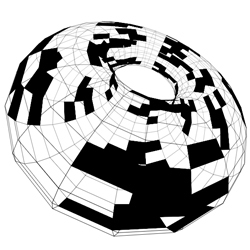
\includegraphics[scale=0.8]{./images/CA_FDM/torus-2}
\caption{3D cellular automata with toroidal cellular space.}
\label{torus}
\end{figure}
This chapter introduces \textit{Cellular Automata} that,  have been proved to be suitable for the modellation and simulation of a wide class of complex physical systems, in particular those ones constructed from \textbf{many identical} components, each (ideally) simple, but together capable of complex behaviour\cite{Toffoli1984,toffoli1987}.
As can be seen from the number of papers in literature  cellular automata have been applied in a wide range of classes of problems from gas\cite{Frisch1986} and fluid turbulence\cite{Succi1991} simulation to macroscopic phenomena\cite{Gregorio1999} like epidemic spread\cite{Sirakoulis2000}, snowflakes and lava flow\cite{dspataro_sciara:2017,Crisci2004,Spataro2010}.
CA were first investigated by \textit{S. Ulam} working on growth of crystals using
lattice network and at the same time by \textit{J. Von Neumann} in order to study
self-reproduction\cite{Neumann1966}; it was not very popular until the 1970 when
the famous \textit{Conway's} game of life\cite{conway1970} appeared, and since then  they have been widely studied from  a theoretical view point until they were proved capable of computational universality\footnote{ Logical gates can be simulated using the simple rules of the \textit{Game of Life} combining special patterns as \textit{gliders} and \textit{guns}}\cite{Thatcher1970}. They have been mainly adopted, after 1980's, as a computational parallel model due to their intrinsically parallel nature\cite{Margolus1986}.


\section{Informal Definition}

Informally a \emph{cellular automata} (CA) is a mathematical model that
consists of a discrete lattice of sites  and a value, the state, that is
updated in a sequence of discrete timestamps (steps) according to some logical rules that
depend on a neighbor  sites of the cell. Hence CA describe systems whose the
overall behavior and evolution of the system may be exclusively described on the basis of local
interactions\cite{wolfram1984}, property also called centrism.
The most stringent and typical characteristic of the CA-model is the restriction
that the local function does not depend on the time t or the place i: a cellular automaton has homogeneous
space/time behavior. It is for this reason that ca are sometimes referred to as
\textit{shift-dynamical} or \textit{translation invariant} systems. From another
point of view we can say that in each lattice site resides a finite state
automaton\footnote{A simple and well know computational model. It has inputs,
outputs and a finite number of states (hence a finite amount of memory);
An automata changes state at regular time-steps.}  that take as
input only the states of the cells in its neighborhood (see figure \ref{amod3Automata}).

\subsection{Cellular space dimension and geometry}
The cellular space is a \emph{discrete} d-dimensional lattice of sites (see
figure \ref{spazioCellulare}).
For 1-D automaton the only way to discretize the space is in a one-dimensional
grid. For automaton with dimensionality higher than 1 the shape of each cell can
be different than squared. In 2D tessellation for example each cell can be
hexagonal or triangular instead of squared. Each tessellation present advantages
and disadvantages. For instance the squared one does not give any graphical
representation problem\footnote{Each cell could be easily mapped onto a
pixel.}, but present problems of anisotropy for some kind of
simulations\footnote{The HPP model for fluid simulation was highly anisotropyc due to the squared tessellation.}\cite{Frisch1986}.
An Hexagonal tessellation can solve the anisotropy problem\cite{wolfram1986} but
presents obvious graphical issues. Often, to avoid complications
due to a boundary, periodic boundary conditions are used, so that a two-dimensional grid
is the surface of a torus (see picture \ref{torus}).


\subsection{Neighborhood}
\begin{figure}
\centering
\caption{Examples of cellular spaces. (a) 1-D, (b) 2-D squared cells,
(c) 2-D hexagonal cells, (d) 3-D cubic cells.}\label{spazioCellulare}
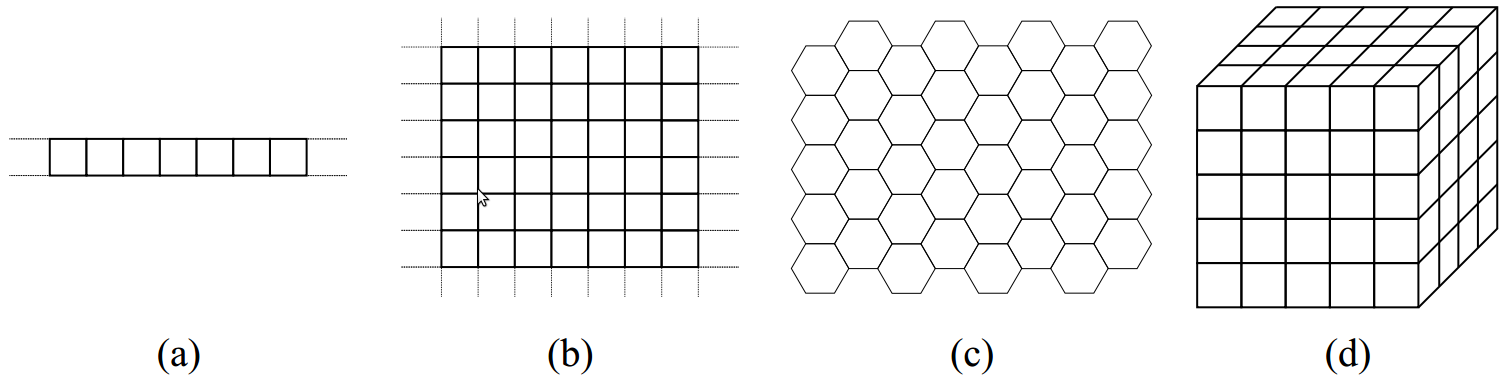
\includegraphics[scale=0.23]{./images/CA_FDM/spazioCellulare}
\end{figure}
The evolution of a cell's state is function of the states of the neighborhood's
cells. The geometry and the number of cells that are part of the neighborhood
depends on the tessellation type, but it has to have three fundamental
properties:
\begin{enumerate}
  \item \textbf{Locality}. It should involve only a 'limited' number of cells.
  \item \textbf{Invariance}. It should not be changed during the evolution.
  \item \textbf{Homogeneity}. It has to be the same for each cell of the
  automaton.
\end{enumerate}
Typically neighborhood ``surrounds'' the central cell. For 1-D cellular automata
its borders are identified with a number \begin{math}r \end{math} called
\textit{radius}\cite{wolfram1983}. A \begin{math}r=2\end{math} identify
\begin{math}n=2r+1\end{math} cells in a 1D lattice: the central cell plus the
right and left cells. Typical 2D cellular space neighborhood are the those of
Moore and von Neumann neighborhood. The number of cells in the Moore
neighborhood of range r is the odd squares \begin{math}(2r+1)^2,\end{math} the
first few of which are 1, 9, 25, 49, 81, and so on as r is increased.
Von Neumann's one consist of the central cell plus the cell at north, south,
east, and west of the central cell itself. Moore's (\begin{math}r=1\end{math})
one add  the farther cells at north-east, south-east, south-west and north-west
(see figure \ref{mooreNeigh}).



\begin{figure}
\centering
\caption{Examples of different kind of neighborhood with
different radius values.}\label{mooreNeigh}
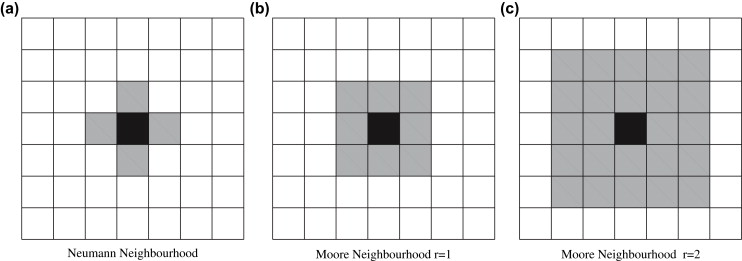
\includegraphics[width=1.0\textwidth]{./images/CA_FDM/mooreNeigh}
\end{figure}

\subsection{Transition Function}
The evolution of the cell's state is decided by the transition function that
is applied at the same time and on each cell. Usually that transition function
is deterministic and defined by a \textit{look-up} table only when the total
number of state for each cell is small\footnote{Otherwise the dimension of that table would be enormous because the number of entries is exponential in the number of
states.} otherwise is defined by an algorithmic procedure.
It may be probabilistic, in the case of stochastic cellular automata.

\section{Formal Definition}
Cellular automata are dynamic models that are
discrete in time, space and state. A simple cellular
automaton A is defined by a lattice of cells each containing a finite state
automaton so we briefly give its definition.

\subsection{Finite State Automaton}\label{DFA}
Also known as deterministic finite automata (DFAs) or as deterministic finite
state machines, are ones of the most studied and simple computational model
known.
 It is a theoretical model of computation\footnote{Language recognition
problem solvers.} that can be in a finite number of states, only one at a time,
the current state. Its state can change in response of inputs taken by a
transition function that describe the state change given the current state and
\begin{table}
\scalebox{1.2}{
\begin{tabular}{|c|ccccc|}\hline
\(\delta\) & \(a\) & \(b\) & \(c\) & \(d\) & \(e\) \\ \hline
\(q_0\) &\(q_0\) &\(q_0\) &\(q_2\) &\(q_1\) &\(q_1\)\\  
\(q_1\) &\(q_1\) &\(q_3\) &\(q_1\) &\(q_1\) &\(q_1\)\\  
\(q_2\) &\(q_3\) &\(q_2\) &\(q_2\) &\(q_0\) &\(q_1\)\\  
\(q_3\) &\(q_0\) &\(q_1\) &\(q_1\) &\(q_0\) &\(q_1\) \\ 
\hline 
 \end{tabular}
}
 \caption{Tabular representation of a DFM's next-state function}
 \label{tab:tabularTransitionFunction}
\end{table} 
the received input of the automata.
Its a much more restrictive in its capabilities than a Turing
machines,\footnote{For example we can show that is not possible for an
automaton to determine whether the input consist of a prime number of symbols.}
but they are still capable to solve simpler problems, and hence to recognize
simpler languages, like well parenthesized string; More in general they are capable
to recognize the so called \emph{Regular languages}\footnote{Languages
defined by regular expressions and generated by regular grammar, Class 3 in
Chomsky classification. We can prove that for each language L accepted by a DFA
exists a grammar \begin{math}L_G \end{math} s.t. \begin{math} L=L_G\end{math}},
but they fail for example in parsing \emph{context-free} languages.
More formally a DFA is a 5-tuple:
\[M = <Q,\Sigma,\delta,q_0,F>\] 

\begin{itemize}
  \item \textit{Q} is a finite, nonempty, set of states.
\item \begin{math}\Sigma\end{math} is the alphabet
\item \begin{math} \delta : Q \times \Sigma \longmapsto Q  \end{math} is the
transition function (also called next-state function, may be represented in
tabular form  (see table
\ref{tab:tabularTransitionFunction})
\item \begin{math}q_0 \end{math} is the initial (or starting) state :
\begin{math} q_0 \in  Q \end{math}
\item  \begin{math}F \end{math} is the set, possibly empty, of final states :
\begin{math} F \subseteq Q \end{math}

\end{itemize}



A run of DFA on a input string \begin{math}u = a_0,a_1,\ldots,a_n\end{math} is a
sequence of states \\ \begin{math} q_0,q_1,\ldots,q_n\end{math} s.t.
\begin{math}q_i  \overset{a_i}{\longmapsto} q_{i+1} \end{math},
\begin{math} 0 \leq i \le n\end{math}. It means that for each couple of state
and input the transition function deterministically return the next DFA's
state \\ \begin{math}q_i=\delta(q_{i-1},a_{i}) \end{math}.
For a given word \begin{math}\textit{w}\in \Sigma^* \end{math} the DFA has a
unique run (it is deterministic), and we say that it \textbf{accepts} w if the
last state \begin{math}q_n \in F \end{math}. A DFA recognizes the
language L(M) consisting of all accepted strings.


Figure \ref{amod3Automata} is an example of DFA\footnote{Graph representation
is the most common way to define and design DFA. Nodes are the states, and
the labelled edges are the possible states transition from a state \textit{u}
to a state \textit{w} given a certain input.
Note that, because the automaton is deterministic is not possible for two
edges to point to two different nodes if same labelled.}.
It accepts the language made up of strings with a number N s.t \begin{math}N
\;mod\; 3 = 0 \end{math}
\begin{itemize}
  \item\begin{math} \Sigma = \{a,b\}\end{math}
  \item \begin{math} Q = \{t_0,t_1,t_2\}\end{math}
  \item \begin{math} q_0 = t_0\end{math}
  \item \begin{math} F = \{t_0\} \end{math}
\end{itemize}


If we execute the DFA on an input string S=\{aaabba\} we can see that at time
t=0 the DFA is in the initial state \begin{math}t_0\end{math} and the first
symbol of S is read.
The transition function is applied once per each symbol is S
(i.e. \begin{math}\left\vert{S}\right\vert\end{math}). The only rule that match 
the current state and input is \begin{math}\delta=(t_0,a)=t_1 \end{math} hence the
new state is \begin{math}t_1\end{math}. The DFA accept the string only if  there
is not any input left and the current state is the final state
\begin{math}q_f\end{math}\footnote{Previously we stated that F was a set but
we can assume that there is only one final state
(\begin{math}\left\vert{F}\right\vert=1\end{math}), because it is easy prove
that exist a DFA with only one final state given a generic DFA
(\begin{math}\left\vert{F}\right\vert \geq 1\end{math}). We add one more state
\begin{math}q_f\end{math} and for each final state \begin{math}q_i \in
F\end{math} we define new rules of the type \begin{math}\delta(q_i,*)=q_f, * \in I \end{math}.}.
S is not accepted by the DFA defined in the example \ref{amod3Automata} because
at the end of the computation the reached state is \begin{math}t_1\end{math}
that is not a final state.
 \[
 t_0\overset{\delta(t_0,a)}
 {\longmapsto}t_{1}\overset{\delta(t_1,a)}
 {\longmapsto}t_{2}\overset{\delta(t_2,a)}
 {\longmapsto} t_{0}\overset{\delta(t_0,b)}
 {\longmapsto}t_{0}\overset{\delta(t_0,b)}
 {\longmapsto}t_{0}\overset{\delta(t_0,a)}
 {\longmapsto} t_{1}
\]
On the input \begin{math}S^1=\{abababb\}\end{math} the DFA accept:
 \[
 t_0\overset{\delta(t_0,a)}
 {\longmapsto}t_{1}\overset{\delta(t_1,b)}
 {\longmapsto}t_{1}\overset{\delta(t_1,a)}
 {\longmapsto} t_{2}\overset{\delta(t_2,b)}
 {\longmapsto}t_{2}\overset{\delta(t_2,a)}
 {\longmapsto}t_{0}\overset{\delta(t_0,b)}
 {\longmapsto}t_{0}\overset{\delta(t_0,b)}
 {\longmapsto}\mathbf{t_{0}}
\]
\begin{figure}
\begin{center}
  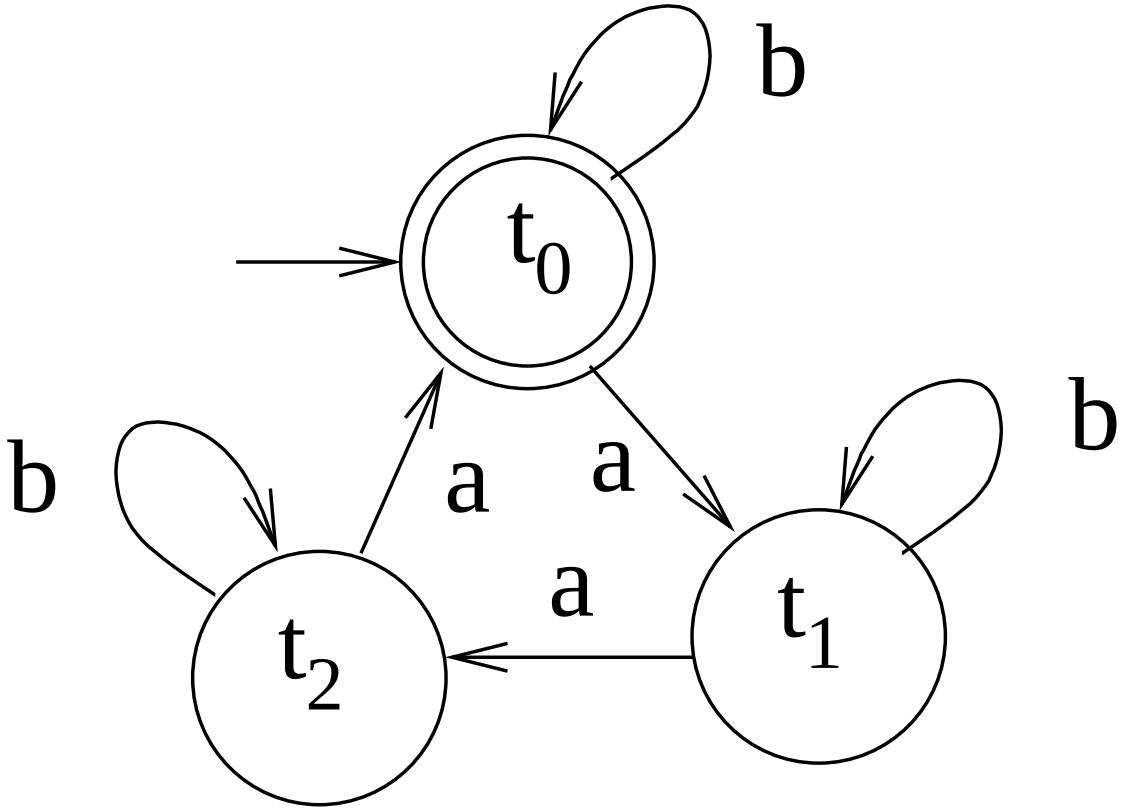
\includegraphics[scale=0.17]{./images/CA_FDM/amod3Automata}
  \caption{Graph representation of a DFA}
  \label{amod3Automata}
\end{center}
\end{figure}



\section{Homogeneous Cellular Automata}\label{homogeneousCellularAutomata}
Formally a CA \emph{A} is a quadruple \begin{math} A=<Z^d,X,Q,\sigma>\end{math}
where:
\begin{itemize}
  \item \begin{math}\mathbb{Z}^d=\{i=(i_1,i_1,\ldots,i_d)\mid i_k \in
  \mathbb{Z}, \forall k=1,2,\ldots,d \}\end{math} is the set of cells of the d-dimensional
   Euclidean space.
  \item \begin{math}X\end{math} is the neighborhood, or neighborhood template; a
  set of m d-dimensional vectors (one for each neighbor)
  \[\xi_j=\{\xi_{j1},\xi_{j2},\ldots,\xi_{jd}\} \;,\: 1\leq j \leq m\] that
  defines the set of the neighbors cells of a generic cell
  \begin{math}i=(i_1,i_1,\ldots,i_d)\end{math}
  \[
  N(X,i)=\{i+\xi_0,i+\xi_2,\ldots,i+\xi_d\}
  \] where \begin{math}\xi_0\end{math} is the null vector. It means that the
  cell \begin{math}i\end{math} is always in its neighborhood and we refer to it
  cell as \emph{central cell}  (see example below).
\item Q is the finite set of states of the elementary automaton EA.
  
  \item \begin{math}\sigma=Q^m \rightarrow Q \end{math} is the transition
  function of the EA. \begin{math}\sigma\end{math} must specify
  \begin{math}q_k \in Q \end{math} as successor  state of the central cell.
  If there are \begin{math}m\end{math} cells in the neighborhood of the central
  cell including itself, then there are
  \begin{math}{\left\vert{Q}\right\vert}^m\end{math} possible neighborhood's
  state configuration. It  means that there are
  \begin{math}{\left\vert{Q}\right\vert}^{{\left\vert{Q}\right\vert}^m}\end{math}
  possible transition functions. Plus we can see that the tabular definition of
  the next-state function is unsuitable for practical purpose. It should have
  \begin{math}\left\vert{\sigma}\right\vert={\left\vert{Q}\right\vert}^m\end{math}
  entries, an exceedingly large number.
  \item \begin{math}\tau=C \longrightarrow C \longmapsto
  \sigma(c(N(X,i))) \end{math} where 
  where $C=\{c \colon Z^d
  \rightarrow Q\}$
  is called the set of the possible configuration and 
  \begin{math}
  C(N(X,i)))\end{math} is the set of states of the neighborhood of \textit{i}.
\end{itemize}



For example consider a 2D cellular automata with Moore neighborhood and a
generic cell c=(10,10) and \begin{math}{\left\vert{Q}\right\vert}=5\end{math}
possible state for each cell .
\[X=\{\xi_{0},\xi_{1},\xi_{2},\xi_{3},\xi_{4},\xi_{5},\xi_{6},\xi_{7},\xi_{8}\}
=\]\[=\{(0,0),(-1,0),(0,-1),(1,0),(0,1),(-1,-1),(1,-1),(1,1),(-1,1)\}
\]
Hence the set of the cells belonging to the neighborhood(defined by X) of
c=(10,10) is:
\begin{math}V(X,c)=\{(0,0)+c,(-1,0)+c,(0,-1)+c,(1,0)+c,(0,1)+c,(-1,-1)+c,(1,-1)+c,(1,1)+c,(-1,1)+c\}
\end{math} 
\[=\{(10,10),(9,10),(10,9),(11,10),(10,11),(9,9),(11,9),(11,11),(9,11)\}
\]
and the total number of entries for the tabular definition of the
transition-function is  \begin{math}{\left\vert{Q}\right\vert}^{\left\vert{X}\right\vert}=
5^9=1953125\end{math} and the total number of possible transition functions
is
\begin{math}{\left\vert{Q}\right\vert}^{{\left\vert{Q}\right\vert}^{\left\vert{X}\right\vert}}=
5^{5^9}=5^{1953125}\end{math}.



\section{Theories and studies}

\subsection{Elementary cellular automata}
The most simple AC we can imagine are the elementary cellular
automata\cite{wolfram1983}. They are one-dimensional periodic N cells array
\begin{math}\{C_i \mid 1\leq i \leq N, C_i \in \{0,1\} \}\end{math} each
with 2 possible state (0,1), and rules that depend only on nearest neighbor
value hence a radius r=1 neighborhood with a total number of involved cell
\begin{math}2r+1=2\times1+1=3\end{math} (central, right and left cells).
Since there are only \begin{math}2\times2\times2\times=2^{2r+1}=2^3=8\end{math} possible states for
the neighborhood of a given cell there are a total of
\begin{math}2^{2^3}=2^8=256\end{math} possible elementary automata (each of
which may be identified with a 8-bit binary number\cite{wolfram2002}).

\subsubsection{Wolfram's code}
The transition function  is \begin{math}F(C_{i-1},C_i,C_{i+1})\end{math} is
defined by a look-up table of the form stated in table
\ref{wolframcodeGeneral}, and an example of an instance of a function is given
(rule 110, an important rule on which \cite{cook2004} proved universal
computational power, as Wolfram had conjectured in 1985, and is arguably the
simplest Turing complete system\cite{wolfram2002}) in table
\ref{wolframcodeGeneral}.

\begin{table}
\caption{Encoding of a transition function for a generic elementary CA. On the
right the instance 110.}
\centering
\begin{tabular}{l}
\label{wolframcodeGeneral}

\hfill \\
\hline
  \begin{math}F(1,1,1)=\{0,1\}\end{math}  \\
  \begin{math}F(1,1,0)=\{0,1\}\end{math}  \\
  \begin{math}F(1,0,1)=\{0,1\}\end{math}  \\
  \begin{math}F(1,0,0)=\{0,1\}\end{math}  \\
  \begin{math}F(0,1,1)=\{0,1\}\end{math}  \\
  \begin{math}F(0,1,0)=\{0,1\}\end{math}  \\
  \begin{math}F(0,0,1)=\{0,1\}\end{math}  \\
  \begin{math}F(0,0,0)=\{0,1\}\end{math}  \\
\hline
\end{tabular}
\quad
\begin{math}\overset{instance}{\longrightarrow}\end{math}
\begin{tabular}{l}

\label{wolframcoderule}
\hfill \\
\hline
  \begin{math}F(1,1,1)=0\end{math}  \\
  \begin{math}F(1,1,0)=1\end{math}  \\
  \begin{math}F(1,0,1)=1\end{math}  \\
  \begin{math}F(1,0,0)=0\end{math}  \\
  \begin{math}F(0,1,1)=1\end{math}  \\
  \begin{math}F(0,1,0)=1\end{math}  \\
  \begin{math}F(0,0,1)=1\end{math}  \\
  \begin{math}F(0,0,0)=0\end{math}  \\
\hline
\end{tabular}
\end{table}

More generally Wolfram's code\cite{wolfram1983,wolfram2002} can be calculated 
Conventionally neighborhoods are sorted in non-decreasing order
,(111=7),(110=6),(101=5) etc., and the may be interpreted as a 8-digit number
\[01101110=2^0\times0+2^1\times1+2^2\times1+2^\times1+2^4\times0+2^5\times1+2^6\times1+2^7\times0=110\]


\begin{enumerate}
  \item List and sort in decreasing numerical (if interpreted as number) order
  all the possible configuration of the neighborhood of a given cell.
  \item For each configuration, list the state which the given cell will have,
  according to this rule, on the next iteration.
  \item Interprets the resulting list as binary number and convert it to
  decimal. That  is the Wolfram's code.
\end{enumerate}

Note that is not possible to understand from that code which is the size or the
shape of the neighborhood. Is tacit to suppose that those information are
already known.


\subsection{Wolfram's classification}
Mathematical analysis of CA may be not so straightforward despite their simple
definition. A first attempt to classify CA was attempted by
Wolfram\cite{wolfram2002}. He proposed a set of four classes for CA
classification that are the most popular method of CA classification, but they
suffer from a degree of subjectivity. Classification is based only on visual
valuations, that are obviously subjective. A more rigorous definition of these
classes is given in \footnote{They prove that decide the class(from the
wolfram's four one) of membership of a generic CA is an undecidable problem. Is
not possible to design an algorithm that solve this problem.}\cite{culik1998}.
Here the four Wolfram's classes.
\begin{enumerate}
  
  \item these CA have the simplest behavior; almost all initial conditions
  result in the same uniform initial state (homogeneous state).
  \item different initial conditions yield different final patterns, but
  these different patterns consist of an arrangement of a certain set of
  structures, which stays the same forever or repeats itself within a few
  steps(periodic structures).
  \item behavior is more complicated and appears random, but some repeated
  patterns are usually present (often in the form of triangles)(chaotic pattern).
  \item in some respects these are the most complicated class; these behave
  in a manner somewhere in between Class II and III, exhibiting sections
  both of predictable patterns and of randomness in their pattern
  formation(complex structures).
\end{enumerate}
He observed that the behavior of a meaningful class of Cellular Automata
by performing computer simulations of the evolution of the automata starting
from random configurations. Wolfram suggested that the different behavior of
automata in his classes seems to be related to the presence of different types
of attractors. In figures \ref{class12} and \ref{class34} some elementary automata divided in their classes.\footnote{Images courtesy of
\url{http://plato.stanford.edu/entries/cellular-automata/}}
 \begin{figure}
 \caption{Class 3 (a,b) and 4 (c,d) elementary cellular automata}
 \label{class34}
\centering
    \begin{subfigure}[b]{0.275\textwidth}
		\centering
		\caption[]{}
		\label{fig:34first}
		
		
\includegraphics[scale=0.32]{./images/CA_FDM/rule250}
\caption[]{}%
   \end{subfigure}%
    \begin{subfigure}[b]{0.275\textwidth}
		\centering
		
\includegraphics[scale=0.32]{./images/CA_FDM/rule254}
		\caption[]{}%
   \end{subfigure}%
   \hfill
       \begin{subfigure}[b]{0.275\textwidth}
   	\centering
   	
\includegraphics[scale=0.32]{./images/CA_FDM/rule4}
   	\caption[]{}%
   \end{subfigure}%
   \begin{subfigure}[b]{0.275\textwidth}
   	\centering
   	
\includegraphics[scale=0.32]{./images/CA_FDM/rule108}
   \caption[]{}%
   \end{subfigure}%
        
\end{figure}

We can well see from these examples that automata from class 1 have all cells
ending up very quickly with the same value, in a homogeneous state and automata
from class 2 with a simple final periodic patterns.
Class 3 appear to be chaotic and non-periodic and automata from class 4 have
a mixed behaviour, complex-chaotic structures are locally propagated.
\subsection{At the edge of Chaos}
Class 4 automata are at \emph{the edge of chaos} and give a good metaphor for
the idea that the \textit{interesting} complexity (like the one exhibit by
biological entities and their interactions or analogous to the phase transition
between solid and fluid state of the matter, is in equilibrium between
stability and chaos\cite{Langton1990}.

\begin{quotation}
\em Perhaps the most exciting implication (of CA representation of biological
phenomena) is the possibility that life had its origin in the vicinity of a
phase transition and that evolution reflects the process by which life has
gained local control over a successively greater number of environmental
parameters affecting its ability to maintain itself at a critical balance point
between order and chaos.\\
(\textit{\textbf{Chris Langton} - Computation at the edge of chaos.
Phase transition and emergent computation - pag.13}).
\end{quotation}

 \begin{figure}
	\caption{Class 3 (a,b) and 4 (c,d) elementary cellular automata}
	\label{class12}
	\centering
	\begin{subfigure}[b]{0.275\textwidth}
		\centering
		\label{fig:first}
		
		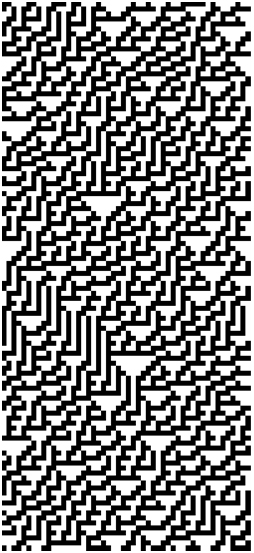
\includegraphics[scale=0.32]{./images/CA_FDM/rule30}
		\caption[]{}%
	\end{subfigure}%
	\begin{subfigure}[b]{0.275\textwidth}
		\centering
		
\includegraphics[scale=0.32]{./images/CA_FDM/rule90}
		\caption[]{}%
	\end{subfigure}%
	\hfill
	\begin{subfigure}[b]{0.275\textwidth}
		\centering
		
\includegraphics[scale=0.32]{./images/CA_FDM/rule54}
		\caption[]{}%
	\end{subfigure}%
	\begin{subfigure}[b]{0.275\textwidth}
		\centering
		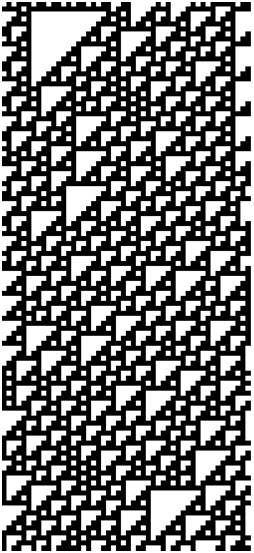
\includegraphics[scale=0.32]{./images/CA_FDM/rule110}
		\caption[]{}%
	\end{subfigure}%
	
\end{figure}



%%
% -------------- End of figure environment ----------------------%


Langton in his famous paper, \textit{Computation at the edge of chaos: phase
transition and emergent computation}\cite{Langton1990},was able to
identify, simply parametrizing the rule space, the various AC classes, the
relation between them and to ``couple'' them with the classical complexity classes.
He introduced the parameter \begin{math}\lambda\end{math}\cite{LangtonThesis1990}that, informally, is simply
the fraction of the entries in the transition rule table that are mapped  the
not-quiescent state.
\[\lambda=\frac{K^N-n_q}{K^N}\]
where:
\begin{itemize}
  \item K is the number of the cell states
  \item N the arity of the neighborhood
  \item \begin{math}n_q\end{math} the number of rules mapped to the quiescent
  state \begin{math}q_q\end{math}
\end{itemize}

\begin{figure}
\centering
\caption{Relation between lambda parameter and the CA
behaviors-Wolfram's classes.}\label{lambdaWolframClass}
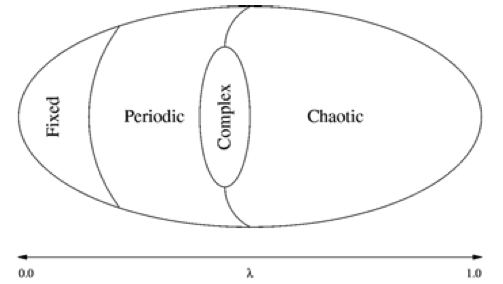
\includegraphics[scale=0.4]{./images/CA_FDM/edgeofchaos}
\end{figure}
Langton's major finding was that a simple measure such as it correlates with the
system behavior: as it goes from 0 to \begin{math} 1-\frac{1}{K}\end{math}(respectively the most
homogeneous and the most heterogeneous rules table scenario), the average
behavior of the system goes from freezing to periodic patterns to chaos and functions with an average 
value of \begin{math}\lambda\end{math} (see \cite{Langton1990} for a
more general discussion) are being on \emph{on the edge}(see figure \ref{lambdaWolframClass}).

He studied a entire family of totalistic CA with \begin{math}k=4
\end{math} and \begin{math}N=5\end{math} with \begin{math}\lambda\end{math}
varying in \begin{math}[0,0.75]\end{math}. He was able to determine that values
of \begin{math}\lambda\approx0.45\end{math} raise up to class 4 cellular
automata.
Computational system must to provide fundamental properties if it is
to support computation. Only CA  \emph{on the edge} show these properties on
manipulating and store information data.
Here the properties that a computational system as to provide:
\begin{description}
  \item[Storage] \hfill \\
  Storage is the ability of the system of preserving information for
arbitrarily long times
  \item[Transmission] \hfill \\
  Transmission is the propagation of the information in the
form of signals over arbitrarily long distance
  \item[Modification] \hfill \\
Stored and transmitted
information is the mutual possible modification of two signals.

\end{description}

Storage is coupled with less entropy of the system, but transmission and
modification are not. Few entropy is associated with CA of Class 1 and 2 and
high entropy with class 3. Class 4 is something in between, the cells cooperate
and are correlate each other, but not too much otherwise they would be overly
dependent with one mimicking the other supporting computation in all its aspects
and requirements. Moreover class 4 CA are very dependent from the initial
configuration opening to the possibility to encode programs in it.

\subsection{Game of life}
\label{sect:GOL}
CA are suitable for representing many physical, biological, social and other
human phenomena. But they are a good tool to study under which condition a
physical system supports the basic operation constituting the capacity to
support computation. Game of life is a famous 2D
cellular automaton of '70s early studied (and perhaps proved) for its universal
computation capacity.



\subsubsection{Game of life - brief definition} 
The Game of Life is totalistic CA\footnote{A totalistic cellular automaton is a cellular automata in which the rules depend only on the	total (or equivalently, the average) of the values of the cells in a neighborhood.} that can be thought as an infinite two-dimensional orthogonal grid of square cells, each of which is in one of two possible states, \emph{dead} or \emph{alive}. Every cell interacts with the eight adjacent neighbors belonging to the Moore neighborhood. At each time step, one of the following transitions occur:
	\begin{itemize}
	\item \emph{Birth}: If the cell is in the state \textbf{\textit{dead}} and
	the number of alive neighbors is \textbf{\textit{3}}, then the cell state
	becomes alive (1).
	\item \emph{Survival}: If the cell is in the state \textbf{\textit{alive}}
	and the number of alive neighbors is \textbf{\textit{2 or 3}}, then the cell
	state is still alive (1).
	\item \emph{Dead}: If the cell is in the state \textbf{\textit{alive}} and
	the number of alive neighbors is \textbf{\textit{less than 2 or higher
			than 3}}, then the cell state becomes dead (0).
\end{itemize}
The initial configuration of the system specifies the state (dead
or alive) of each cell in the cellular space. The evolution of the
system is thus obtained by applying the above rules (which define
the cell's transition function) simultaneously to every cell in
the cellular space, so that each new configuration depends on the
one at the current step. The rules continue to be applied
repeatedly to create further generations.

Formally the Game of Life CA can be defined as follows:
$$Life = < R, X, Q, \sigma >$$ where:
\begin{itemize}
	\item $R$ is the set of points, with integer coordinates, which
	defines a two-dimensional toroidal cellular space. The generic
	cell in $R$ is individuated by means of a couple of integer
	coordinates $(i, j)$, where $0 \leq i < i_{max}$ and $0 \leq j <
	j_{max}$. The first coordinate, $i$, represents the row, while
	the second, $j$, the column. The cell at coordinates $(0,0)$ is
	located at the top-left corner of the computational grid
	(cf. Figure \ref{fig:2Dneighborhood}b).
	
	\item $X = \{(0,0), (-1, 0), (0, -1), (0, 1), (1, 0), (-1,-1),
	(1,-1), (1,1), (-1,1)\}$ is the Moore neighborhood relation. The
	neighborhood coordinates of the generic cell of coordinate $(i,
	j)$ is given by
	$$N(X, (i, j)) = $$
	$$= \{(i, j)+(0,0), (i, j)+(-1, 0), \dots, (i, j)+(-1,1)\} =$$
	$$= \{(i, j), (i-1, j), \dots, (i-1,j+1)\}$$ Here, a subscript
	operator can be used to index cells belonging to the
	neighborhood. Let $|X|$ be the number of elements in X, and $n
	\in \mathbb{N}$, $0 \leq n < |X|$; the notation
	
	$$N(X, (i, j), n)$$
	
	represents the coordinates of the $n^{th}$ neighborhood of the
	cell $(i,j)$. Thereby, $N(X, (i, j), 0) = (i, j)$, i.e. the
	central cell, $N(X, (i, j), 1) = (i-1, j)$, i.e. the first
	neighbor, and so on (cf. Figure \ref{fig:2Dneighborhood}b).
	
	\item $Q = \{0, 1\}$ is the set of cell states, 0 representing the
	dead state, 1 the alive one.
	
	\item $\sigma : Q^9 \rightarrow Q$ is the deterministic cell
	transition function. It is composed by one elementary process,
	which implements the aforementioned transition rules.
\end{itemize}

The Game of Life is a class 4 Wolfram's taxonomy CA, because
\say{rich and complex structures, stable blocks and moving patterns come into existence even starting from a completely random configuration}. 
\begin{figure}
\centering
\caption{GOL execution example.}
\label{gameoflife}
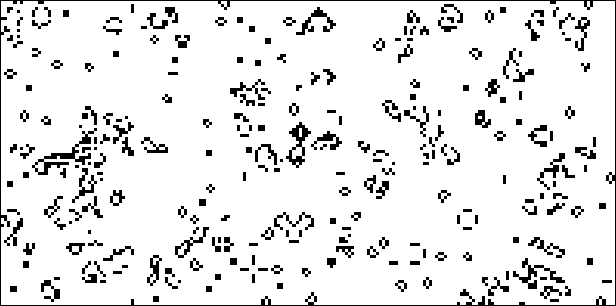
\includegraphics[width=1.0\textwidth]{./images/CA_FDM/game-of-life}
\end{figure}
A famous block for example is the \emph{glider} ( see picture \ref{fig:glider}) that is a 5-step-period pattern that is capable of moving into the cellular space.

\subsubsection{Game of life as Turing machine}
Every CA con be considered a device capable of supporting computation and the
initial configuration can encode an input string (a program for example). At
some point the current configuration can be interpreted as the result of the
computation and decoded in a output string. But as we stated before in section
\ref{DFA} not all the computational device have the same computational power. So
which is the one of the game of life? Life was proved can compute everything a
universal Turing machine can, and under Turing-Church's thesis, everything can
be computed by a computer\cite{berlekamp1982}.
\begin{figure}
\centering
\caption{Glider in Conway's game of life.}
\label{fig:glider}
\setlength{\fboxrule}{1pt}%
\fbox{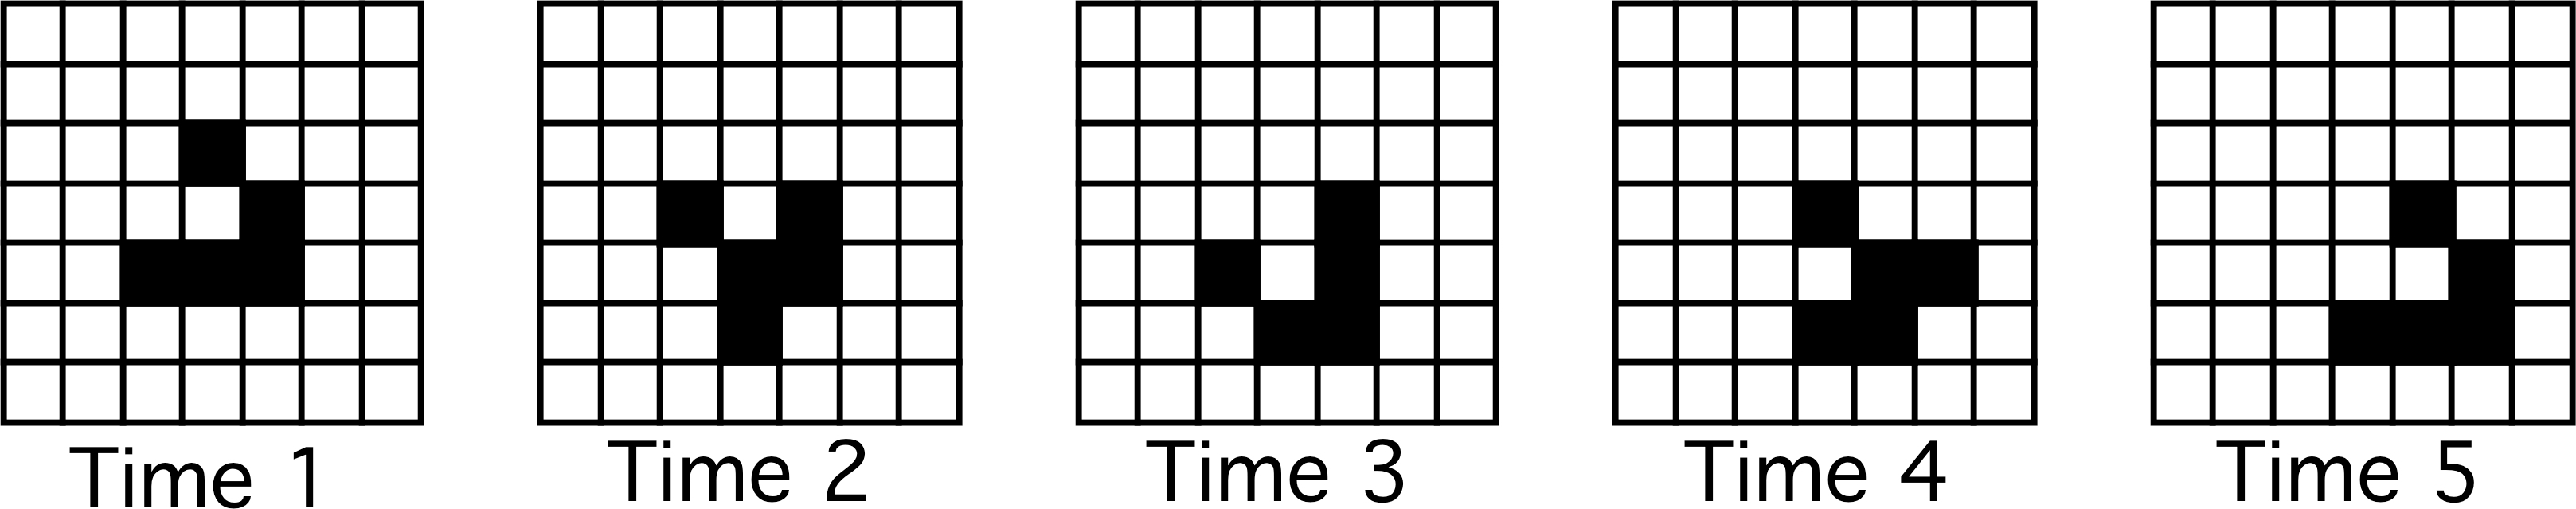
\includegraphics[width=1.0\textwidth]{./images/CA_FDM/glider}}
\end{figure}



This raises a computational issue; given the \emph{Halting
Theorem}\footnote{There can not be any algorithm to decide whether, given an
input, a Turing machine will accept or not.} the evolution of \emph{Life} is
unpredictable (as all the universal computational systems) so it means that is
not possible to use any algorithmically shortcuts to anticipate the resulting
configuration given an initial input. The most efficient way is to let the
system run.

\begin{quotation}
\em Life, like all computationally universal systems, defines the most efficient
simulation of its own behavior\cite{Ilachinski2001}
\end{quotation}





\section{Extension of the Cellular automata model}
It is possible to relax some of the assumptions in the general characterization
of CA provided in the ordinary CA definitions and get interesting results.
Asynchronous updating of the cell, non homogenous lattice with different
neighborhood or transition functions.

\subsection{Probabilistic CA}
Probabilist CA is are an extension of the common CA paradigm. They share all
the basic concept of an ordinary homogeneous
CA with an important difference in the transition function.
\begin{math}\sigma\end{math} is a stochastic-function that choose the next-state
according to some probability distributions. They are used in a wide class of
problems like in modelling ferromagnetism, statistical mechanics
\cite{Vichniac1984} or the cellular Potts model\footnote{Is a computational
lattice-based model to simulate the collective behavior of cellular structures.}


\subsubsection{Cellular automata as Markov process}
Another approach in studying CA, even if it is probably not a practical
way to study the CA is to see CA as a Markov process\footnote{Name for the
Russian mathematician Andrey Markov best known for his work on stochastic
processes.}. A Markov process, is a stochastic process that exhibits
memorylessness \footnote{Also called Markov property.} and it means that the
future state is conditionally independent\footnote{Two event
\begin{math}A\end{math} and \begin{math}B\end{math} are independent if
\begin{math}P(A B)=P(A)P(B)\end{math} or in other words that the conditional
probability \begin{math}P(A|B)=P(A)\end{math}.} of the past.
This property of the process means that future probabilities of an event may be
determined from the probabilities of events at the current time.
More formally if a process has this property following  equation holds:
\begin{align*}
P(X(t_n)&= x \,| X\,(t_1) = x_1,X(t_2) = x_2, \ldots,X(t_{n-1})=x_{n-1}) \\
&= P(X(t_n)=x | X(t_{n-1}=x_{n-1})
\end{align*}

In PCA analysis we are more interested in Markov chain because each cell has a
discrete set of possible value for the status variable.
In terms of chain a CA is a process that starts in one of these states and moves
successively from one state to another. If the chain is currently in state
\begin{math}s_i\end{math}, than it evolve to state \begin{math}s_j\end{math} at
the next step with probability \begin{math}p_{ij}\end{math}.The changes of state
of the system are called transitions, and the probabilities associated with
various state changes are called transition probabilities usually represented
in the Markov chain transition matrix :
\[
M =
\left( {\begin{array}{cccc}
p_{11} & p_{12} & p_{13} &\cdots \\
p_{21} & p_{12} & p_{23} &\cdots \\
p_{31} & p_{32} & p_{33} &\cdots \\
\vdots & \vdots  &\vdots& \ddots\\
\end{array} } \right)
\]

This could seems to be a good way to analyze the probabilistic CA but, a
small grid  \begin{math}10\times10\end{math} (common models model use grid
\begin{math}100\times100\end{math} or larger) identify
\begin{math}2^{10\times10}\end{math}possible states and the resulting matrix
dimension of \begin{math}2^{10\times10}\times2^{10\times10}\end{math} that is a
very large number!



%%*******************************************************************************
%***************************** Finite difference Chapter ***********************
%*******************************************************************************

\chapter{The Finite Difference Method}
\label{ch:FDM}
\vskip 1em
\dictum[Bertrand Russel]{%
	All exact science is dominated by the idea of approximation. When a man tells you that he knows the exact truth about anything, you are safe in infering that he is an inexact man.. }%
\vskip 1em
\dictum[John von Neumann]{%
	Truth … is much too complicated to allow anything but approximations. }%
\vskip 1em

\lettrine[lines=3,lhang=0.33,lraise=0,loversize=0.15]{M}{ost} of the Partial Differential Equations (PDE) arising from formulation of physical problems are very hard to solve analytically, requiring approximate numerical solution.
An important part of handling and solving PDEs is to be able to use local,accurate and stable algebraic expression as an approximation of the derivatives appearing in the equations retaining, at the same time, most of the global and continuous information of the original formulation.
During the last half century several methods approximation methods have been developed and studied, such as the finite volume (FV), finite element (FE), and finite difference (FD) methods (FDM), each with specific approaches to discretization. 
This chapter briefly describes the concept of differential equation and introduces their numerical solution using the Finite Difference Method. For a rigorous and complete descritpion of the topic of this chapter please refer to \cite{cita qui un paio di lavori}.

\subsection{Differential Equation}
A differential equation is an equation where the unknown is a function itself and where derivatives ot the unknown appears in the equation \cite{Larsoon:2004} \cite{Mcowen:2002}. Differential Equations can be divided into two main classes:

\begin{description}
\item[Ordinary Differential Equation (ODE)] where the unknown function contains only derivatives with the respect of a single variable. As example of ODE is the following
\[
  \frac{d T}{d x} = \alpha T(x) +b
\] where $a$ and $b$ are some constant.

\item [Partial Differential Equations (PDE)] which is an extremely large and rich of functions class each of them with a different behavior and properties. Examples of classes in of this kind of differential equations are parabolic, elliptic or hyperbolic equations. PDEs search for a multidimensional function of several variables, and this means that partial derivatives may now appears in the equation. 
Examples of famous PDEs are:
   \begin{descritpion}
     \item [Transport Equation:] \hfil \\
     \begin{equation}
		\frac{\partial T}{\partial t} + \frac{\partial T}{\partial x} =0
     \end{equation}
     \item [diffusion equation:]\hfil \\ 
     \begin{equation}
     	\frac{\partial T}{\partial t} - \frac{\partial^2 T}{\partial x^2}=0
     \end{equation} 
     \item [1D wave equation:]\hfil \\  
     	\begin{equation}
     	\frac{\partial^2 T}{\partial t^2} -\frac{\partial^2 T}{\partial x^2}=0
     	\end{equation}
     \item [Laplace's equation:]\hfil \\  
     	\begin{equation}
     	\frac{\partial^2 T}{\partial x^2} + \frac{\partial^2 T}{\partial y^2}=0
     	\end{equation}
     \item [Heat equation:]\hfil \\  
     	\begin{equation}
     	\frac{\partial T}{\partial t} - \kappa \frac{\partial^2 T}{\partial x^2}=0
     	\label{eq:heat_equation}
     	\end{equation}
   \end{descritpion}
\end{description}
Note that there is a missing piece that would allow all these equation to be solved unequivocally. The initial condition and/or boundary. For example, regarding the 1D wave equation, what is the reflection coefficient at the ends of the string? 
Initial condition must be provided whenever the differential equation is time dependent. Boundary conditions must be specified whenever spacial dependency occurs. Boundary conditions specify the behavior of the equation at the boundary of the domain $\partial \Gamma$ (which has to be compact). Most common boundary conditions are of two kind:
\begin{description}
	\item [Dirichlet:] \hfil \\ in which the values of the functions at $\partial \Gamma$ are hard-coded, i.e. $T(\partial \Gamma)$  is known.
	
	\item [Neumann:] specifies values of the derivatives at $\partial \Gamma$.
	
\end{description} 
Other kind of boundary conditions are possible, such as for instance the Robin's boundary conditions which is a mix of Dirichlet and Neumann ones. See Figure \ref{fig:heat2d_bc} for an example of Dirichlet boundary conditions for the equation \ref{eq:heat_equation}.

    \begin{center}
	\begin{figure}
    	\begin{tikzpicture}
    	\node[anchor=south west,inner sep=0] at (0,0) {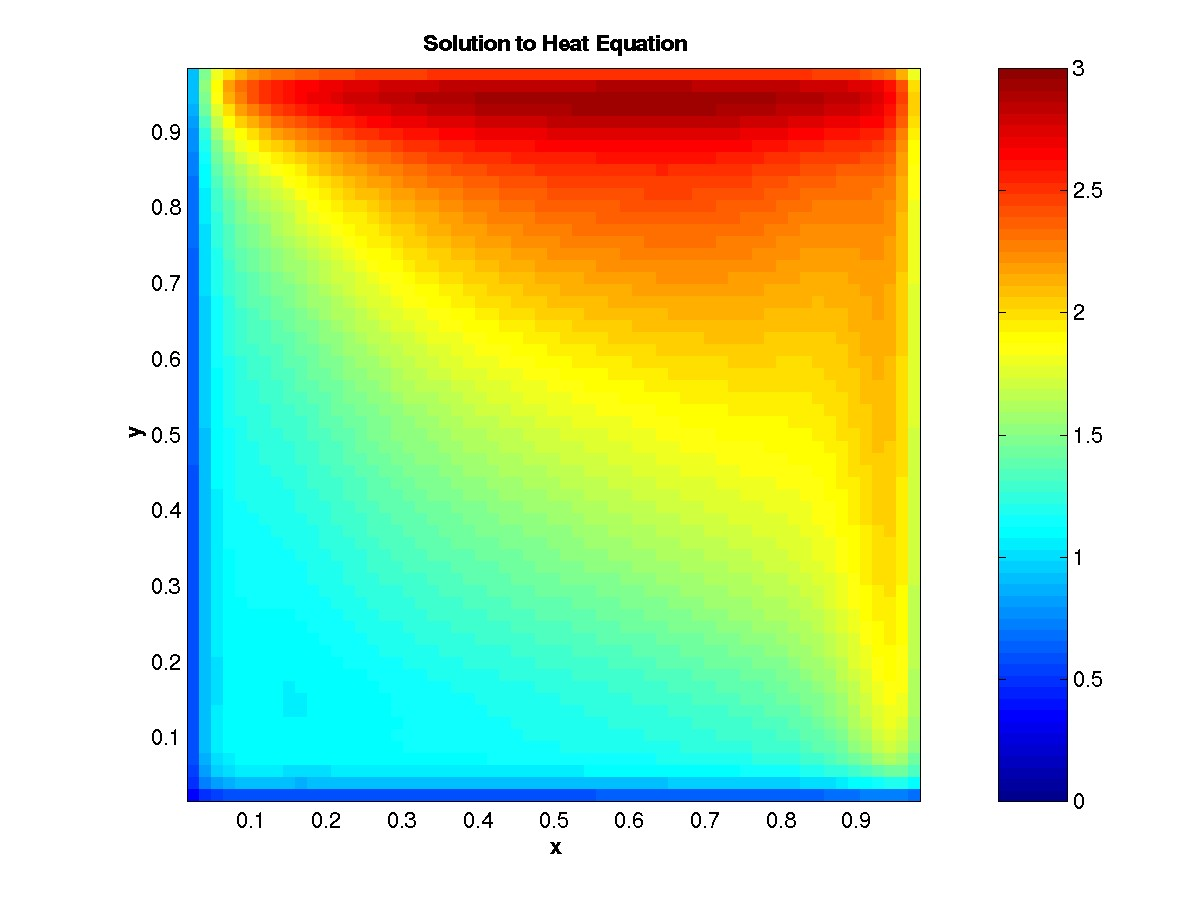
\includegraphics[scale=0.3]{./images/CA_FDM/heat2d_bc}};
    	\draw<1>[red,ultra thick,rounded corners] (1.9,0.94) rectangle (\textheight-14cm,1.3);
    	\draw<1>[red,ultra thick,rounded corners] (1.9,8.94) rectangle (\textheight-14cm,8.6);
    	
    	\draw<1>[red,ultra thick,rounded corners] (1.9,0.8) rectangle (2.3,\textheight-14.7cm);
    	\draw<1>[red,ultra thick,rounded corners] (9.5,0.8) rectangle (9.9,\textheight-14.7cm);
    %	\draw<2>[red,ultra thick,rounded corners] (5.7,4.1) rectangle (7.5,4.9);
   
    	\end{tikzpicture}
    	 \label{fig:heat2d_bc}
    	\caption[Heat Equation Boundary Conditions]{Heat Equation (see Equation \ref{eq:heat_equation}) Dirichlet Boundary Conditions. The perimeter of the square domain (highlighted in red) has fixed temperature, i.e. the solution $T$ is known at the boundary. In particular, $T(x,0)=T(0,y)=0$, $T(1,x)=3$ and $T(1,y)=2$ where $0\leq x,y\leq 1$. }\label{fig:heat2d_bc}
	\end{figure}
\end{center} 

%------------------Finite difference Formulas-------------------------------
    \section{Finite Difference Method}
The finite difference approximation for derivatives is one of the simplest oldest method to solve differential equations numerically. It was used since 1768 by \textit{L. Euler} to solve one dimensional problems and extended by \textit{C. Runge} to two dimension in 1910. Since the advent of computers in 1950, FDM  popularity skyrocketed also thanks to the theoretical results that have been obtained regarding stability, convergence and other of its properties during the last five decades.

The general idea behind FDM is that the differential operator is approximated by replacing the derivatives using difference quotients. The differential operator is approximated constituting the field equation locally, among a number of finite function values. Therefore, the space and time domain are \textit{partitioned} in a grid like fashion in order to store the local field quantities, and approximated solutions are computed only for those discrete grid points. The numerical solution is known only at a finite number of points in the physical domain. 
Difference quotients are linear combination of function values at neighboring grid points. The number of different points appearing in the quotient directly dictates the order ot the differential operator.
We can always assume rectangular grid since we can always  specify boundary conditions for the grid points such that they mimic the real shape of the boundary at hand, (see Figure \ref{fig:gridcustomshape}).
The values of such points that lie on
A refinement on the treatment of complex geometries and curvilinear boundaries is compute the value of such points that lie on the boundary as a linear interpolation of neighboring boundary grid points as shown in Figure \ref{fig:gridcustom_shape2} and Equation \ref{eq:interpolateboundary}.

\begin{equation}
   T(R) = \frac{T_4(h-\delta) + T_0 \delta}{h} = g_0(R)
   \label{eq:interpolateboundary}
\end{equation}
where $g_0$ specifies the values at the boundaries.
\begin{figure}
	\minipage{0.44\textwidth}
	\begin{subfigure}{1.0\textwidth}
		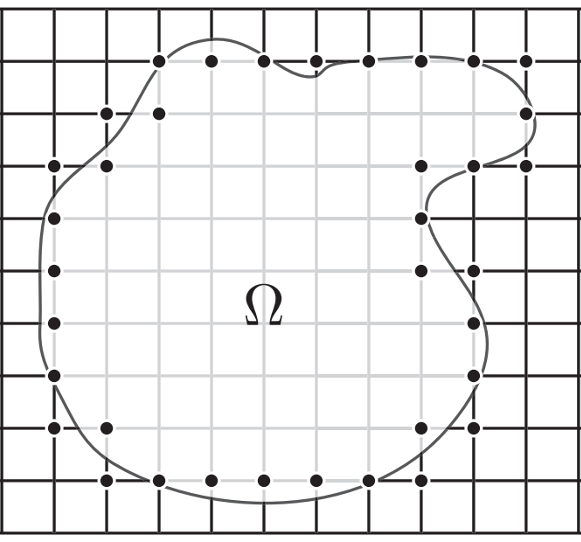
\includegraphics[width=\linewidth]{./images/CA_FDM/grid_custom_shape}
		\label{fig:gridcustomshape}
		\caption{Discretization of a curvilinear domain.}
	\end{subfigure}		
	\endminipage\hfill
	\minipage{0.53\textwidth}
	\begin{subfigure}{1.0\textwidth}
		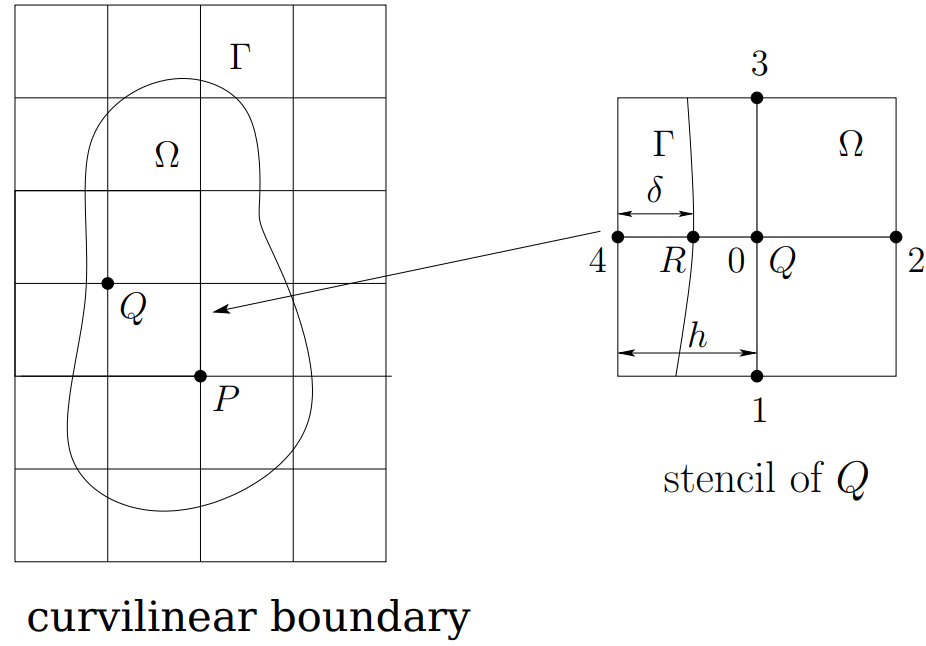
\includegraphics[width=\linewidth]{./images/CA_FDM/gridcustom_shape2}
		\label{fig:gridcustom_shape2}
		\caption{Interpolation of boundary values on a non rectangular geometry domain.}
	\end{subfigure}
	\endminipage\hfill
\end{figure}

Figure \ref{fig:schematic_repr_fdm} is a schematic representation of how FDM are used to obtain a numerical solution. The continuous differential operators and the domain are discretized. The approximation is computed solving the difference formulas on grid points using.

   

\begin{figure}[b]
    \centering
  \begin{tikzpicture}

    \node[draw, text centered,text width=2.5cm] (1) at (0,0) {Continuous PDE};
    \node[draw, text centered,text width=2cm] (2) at (6.5,0) {Discrete Difference Equation};
    \node[draw, text centered,text width=4cm] (3) at (12,0) {$T_j^n$, approximation};

\draw[thick,->] (1) -- (2) node[midway,sloped,above,rotate=0] {\textbf{Finite Difference}};
\draw[thick,->] (2) -- (3) node[midway,sloped,above,rotate=0] {\textbf{Solve}};
\end{tikzpicture}
    \caption{Relationship between continuous and discrete problems.}
    \label{fig:schematic_repr_fdm}
\end{figure}
    
    The error, between the numerical solution and the exact solution is determined by the difference formula utilized and is commonly refeered as \textit{truncation}\footnote{The term truncation comes from the fact that a finite difference quotient is a truncation of the Taylor expansion.} or \textit{discretization} error.  Increasing the resoution of the grid increases the accuracy of the numerical solution since the error associated with the finite difference formulas directly depends on the distance between grid points.
    
        
    Depending on how the derivatives are approximated, explicit or implicit FDM schemes are
    obtained. When forward difference formulas are considered, the
    resulting difference equation is generally expressed in terms of
    an explicit recurrence formula, while backward difference formulas
    generally lead to implicit recurrence formulas involving unknown
    values, and therefore require the solution of a linear system to
    obtain the new state of the system at each grid point.
    
    
\subsection{Finite Difference Formulas}
Differential operator appearing in a PDE problem can be approximated at a given point by a difference formula which is a linear function of its neighboring grid points. There is a number of ways of defining and deriving a finite difference formula but some of them are more widely and commonly used then others. The rest of this section shows how  these common formulas are derived along with their basic properties. 

For the sake of simplicity the formulas are refereed to a one-dimensional space and time domain since the generalization to several dimensions is obvious.
Both space and time domain are partitioned into a finite discrete mesh as follows:    
 \begin{equation}
    		t_n = n\Delta t, \: n = 0,1,\ldots,L,\; \Delta t= \frac{1}{L}
    \end{equation}
    \begin{equation}
    		x_j = j\Delta x, \: j = 0,1,\ldots,M,\;\Delta x = \frac{1}{M}
    \end{equation}

For the rest of the chapter, it can be assumed that grid points are identifies by two indices (see Figure \ref{fig:fdmheatequationstencil}) and $T_j^n$ is the value the function at time $n$ at grid point $j$.

\subsection{Forward Scheme}
    Probably the most common FD formula can be derived from Taylor's expansion of $T^n_{j+1}$ in terms of $T^n_{j}$ and its derivatives as:
    
    \begin{equation}
    T^n_{j+1} = T^n_{j} +
    \frac{\partial T}{\partial x}\bigg\rvert^n_j \Delta x +
    \frac{1}{2!}  \frac{\partial^2 T}{\partial x^2}\bigg\rvert_j \Delta x^2 + \ldots + 
     \frac{1}{k!}  \frac{\partial^k T}{\partial x^k}\bigg\rvert_j \Delta x^k + \ldots
     \label{eq:taylorexp1}
    \end{equation}
    
    If series is truncated after the second term ($k=1$) and solving for $\frac{\partial T}{\partial x}$ the following is obtained:
    
    \begin{equation}
    \frac{\partial T(t,x)}{\partial x}  = \frac{T^n_{j+1} - T^n_{j}}{\Delta x} + \mathcal{O}(\Delta x)
    \label{eq:fdmforward}
    \end{equation}
    
    Equation \ref{eq:fdmforward} is called fist \textbf{forward} finite difference approximation. Other approximations are possible and are easily obtainable by expanding different points of the grids and using more points from the expansion.
    
  \subsection{Backward Scheme}  
    \textbf{Backward} finite difference quotient can be obtained from the Taylor's expansions of    
        \begin{equation}
    T^n_{j-1} = T^n_{j} - 
    \frac{\partial T}{\partial x}\bigg\rvert_j \Delta x +
    \frac{1}{2!}  \frac{\partial^2 T}{\partial x^2}\bigg\rvert_j \Delta x^2 + \ldots + 
     \frac{1}{k!}  \frac{\partial^k T}{\partial x^k}\bigg\rvert_j \Delta x^k + \ldots
     \label{eq:taylorexp2}
    \end{equation}
    
    which can be rearranged in the following manner
        \begin{equation}
    \frac{\partial T}{\partial x}\bigg\rvert_j  = \frac{T^n_{j} - T^n_{j-1}}{\Delta x} + \mathcal{O}(\Delta x)
    \label{eq:fdmfbackward}
    \end{equation}
    
   The same approach can be used to derive approximation for higher order derivatives.
   For example equation \ref{eq:fdmcentral}, known called \textbf{central difference formula}, is an approximation for the second order derivative and can be obtained retaining the firsts four terms in both equations \ref{eq:taylorexp1} and \ref{eq:taylorexp2} and adding the resulting expression:
   
    \begin{equation}
		\frac{\partial^2 T}{\partial x^2}\bigg\rvert_j = \frac{T^n_{j+1}- 2T^n_{j} + T^n_{j-1}}{\Delta x^2} + \mathcal{O}(\Delta x^2)
		\label{eq:fdmcentral}
    \end{equation}
    
    Figure \ref{fig:geometrical_intepretation} show how finite difference formulas can be interpreted geometrically.
\begin{figure}
	\centering
	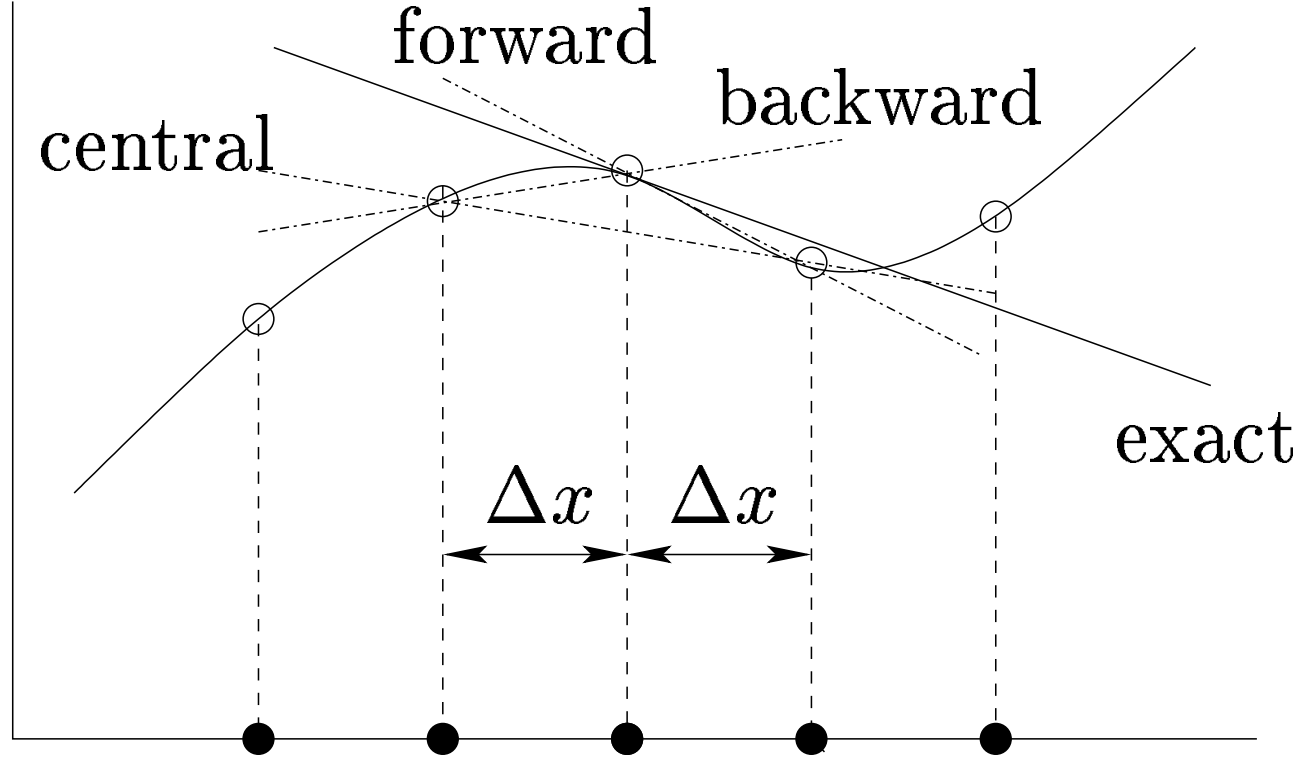
\includegraphics[width=0.85\textwidth]{./images/CA_FDM/geometrical_interpretation_fd}
	\label{fig:geometrical_intepretation}
	\caption{Explicit FDM discretization for the 1D heat conduction problem}\label{torus}
\end{figure} 
    
Note that this approach in deriving FD formulas can be generalized in order to obtain FD approximation for derivatives of any order.

 \subsection{Mixed Derivatives}

Mixed derivatives con also be approximated using FDM, e.g. for two dimensions by means of the following property of mixed derivatives:
\begin{equation}
\frac{\partial ^2 T}{\partial x \partial y} = \frac{\partial}{\partial x} \Bigg{(}\frac{\partial T}{\partial y}\Bigg{)} = \frac{\partial}{\partial y} \Bigg{(}\frac{\partial T}{\partial x}\Bigg{)}\\
\end{equation}
and considering the following approximations:
\begin{equation}
\begin{cases}
&\frac{\partial ^2 T}{\partial x \partial y} = 
\frac{\bigl(\frac{\partial T}{ \partial y}\bigr)_{i+1,j}\, - \,
	\bigl(\frac{\partial T}{ \partial y}\bigr)_{i-1,j}
}{2\Delta x} +\mathcal{O}(\Delta x)^2 \\
&\bigl(\frac{\partial T}{\partial y}\bigr)_{i+1,j} = \frac{T_{i+1,j+1} -T_{i+1,j-1}}{2\Delta y}+\mathcal{O}(\Delta y)^2 \\
&\bigl(\frac{\partial T}{\partial y}\bigr)_{i-1,j} = \frac{T_{i-1,j+1} -T_{i-1,j-1}}{2\Delta y}+\mathcal{O}(\Delta y)^2 \\
\end{cases}
\end{equation}
A second order 2 variables finite difference approximation for the mixed derivative is the following:

\begin{equation}
\Bigg{(}\frac{\partial ^2 T}{\partial x \partial y}\Bigg{)}_{i,j}= \frac{T_{i+1,j+1} -T_{i+1,j-1} - T_{i-1,j+1} -T_{i-1,j-1}}{4\Delta x \Detla y} +\mathcal{O}((\Delta x)^2,(\Delta y)^2)
\end{equation}

Extending the former method to higher dimensional mixed derivatives is straightforward.
    %------------------HEAT Equation-------------------------------
    \section{Heat Equation}
        As an example a simple FDM scheme for an initial-boundary condition problem for the heat conduction problem is derived. 
    
\begin{equation}
    \frac{\partial T(t,x)}{\partial t}= \kappa\frac{\partial^2
      T(t,x)}{\partial x^2}
      \label{eq:heatconduction}
\end{equation}
 
    where $0 \leq t \leq L$ and $0 \leq x \leq
    M$. 
 In order to construct a FD approximation for equation \ref{eq:heatconduction} 
 
 \begin{figure}[b]
 	\centering
 	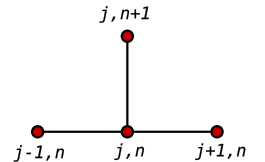
\includegraphics[scale=0.5]{./images/CA_FDM/heatstencil}
 	\label{fig:fdmheatequationstencil}
 	\caption{Explicit FDM discretization for the 1D heat conduction problem}\label{torus}
 \end{figure}   
 
 \begin{enumerate}
 
 \item Discretize the domain into a finite regular mesh where each point $x_j$ is identified with a unique index $j$.
    
 \item  First and second order derivative appearing in \ref{eq:heatconduction} are substituted by forward and central difference formulas, respectively, leading to Equation \ref{eq:discretizedheatequation} (see Figure  \ref{fig:fdmheatequationstencil}):
 
 \begin{equation}
  \frac{T^{n+1}_{j} - T^n_{j}}{\Delta t} = \kappa \frac{T^n_{j+1}- 2T^n_{j} + T^n_{j-1}}{\Delta x^2}
 \label{eq:discretizedheatequation}
 \end{equation}
 
 \item Equation \ref{eq:heatconduction} is evaluated at grid point $(n\Delta t, j \Delta x)$ 
    
\end{enumerate}    
    

    
\begin{figure}
\centering
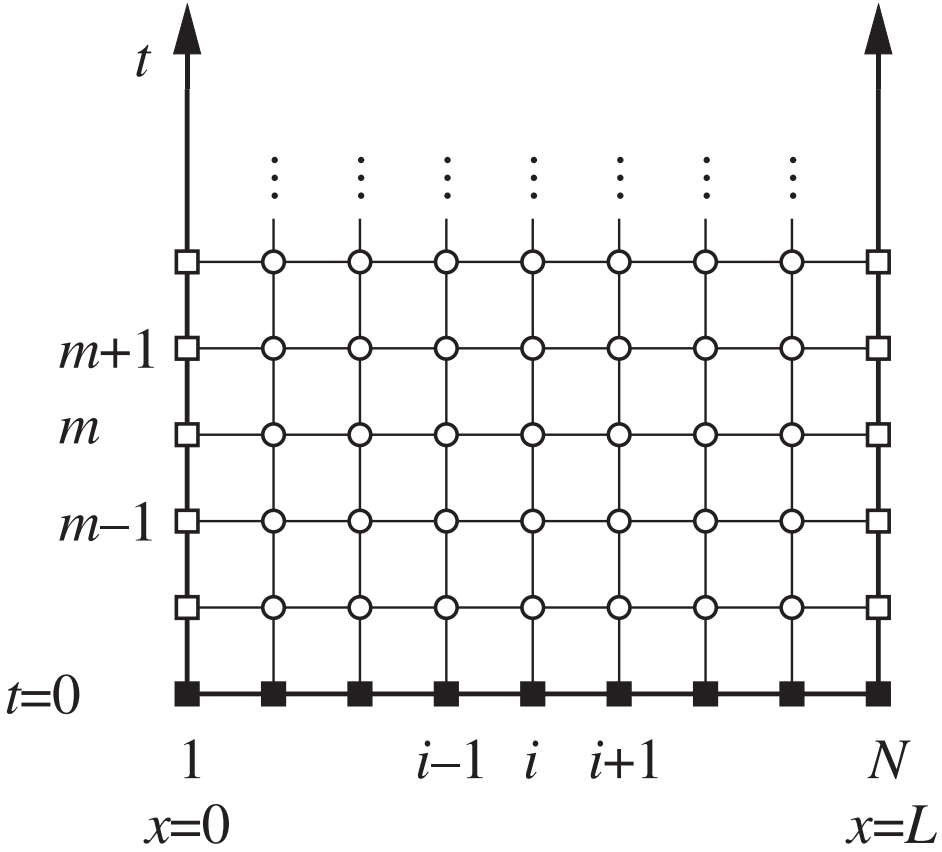
\includegraphics[width=0.8\textwidth]{./images/CA_FDM/fdmgrid}
\caption{1D heat equation FDM grid space and time partitioning.}\label{torus}
\end{figure}

Solution to equation \ref{eq:heatconduction} using the discretization \ref{eq:discretizedheatequation} is called \textit{forward time, centered space or FTCS} approximation and requires the specification of initial conditions at $t=0$ and boundary condition at $x=0$ and $x=M$ (see Figure \ref{fig:heat2d_bc}).

It can be shown that in order to the solution to be stable $\Delta t$ must not be too large and in particular the following condition must hold to ensure a stable solution \cite{isaacson:1994,anderson:1994,crank:1996}:
\[ 
 r= k \frac{\Delta t}{\Delta x^2}< \frac{1}{2}
\]

This scheme is also called explicit because values the the next time are explicitly computable from the values at the current time as it is shown in the equation \ref{eq:discretizedheatequation1}.
 \begin{equation}
  T^{n+1}_{j} = T^n_{j} + \frac{k \Delta t}{\Delta x^2} (T^n_{j+1}+T^n_{j-1}-2T^n_{j})
 \label{eq:discretizedheatequation1}
 \end{equation}

%%backward heat equation
When the backward difference formula is used for approximating the time derivative the following approximation is obtained

 \begin{equation}
  \frac{T^{n}_{j} - T^{n-1}_{}}{\Delta x} = k \frac{T^n_{j+1}- 2T^n_{j} + T^n_{j-1}}{\Delta x^2}
 \label{eq:discretizedheatequation_implicit}
 \end{equation}
 This stepping scheme is called implicit because values at time $n$ are given implicitly as can be seen if equation \ref{eq:discretizedheatequation_implicit} is rearranged to obtain the following: 
 \begin{equation}
T^n_{j} - \frac{k \Delta t}{\Delta x^2} (T^n_{j+1}+T^n_{j-1}-2T^n_{j}) =   T^{n-1}_{j}
 \label{eq:discretizedheatequation1}
 \end{equation}
 In order to obtain values of T at time $n$ a system of non trivial algebraic equation has to be solved. 
 It can be rewritten in matrix form yielding to a tridiagonal matrix (see Section \ref{sec:tridiagonal})

\begin{equation}
\begin{tikzpicture}[baseline=(current bounding box.center)]
\matrix (m) [matrix of math nodes,nodes in empty cells,right delimiter={]},left delimiter={[} ]{
  (1+2\lambda)  & -\lambda     &          &  &  &  & &  \\
  -\lambda      & (1+2\lambda) & -\lambda &  &  &  & & \\
  &             &              &          &  &  &  & & \\
  &             &              &          &  &  &  & & \\
  &             &              &          &  &           &             &           \\
  &             &              &             &    -\lambda &(1+2\lambda) & -\lambda \\
  &             &              &          &  &           &  -\lambda   &(1+2\lambda) \\
} ;
\draw[line width=1pt,line cap=round,loosely dotted] (m-2-2)-- (m-6-6);
\draw[line width=1pt,line cap=round,loosely dotted] (m-2-3)-- (m-6-7);
\draw[line width=1pt,line cap=round,loosely dotted] (m-2-1)-- (m-6-5);
\end{tikzpicture}
\begin{tikzpicture}[baseline=(current bounding box.center)]
\matrix (m) [matrix of math nodes,nodes in empty cells,right delimiter={]},left delimiter={[} ]{
	 T_1^n  &   \\
	T_2^n   &  \\
			&\\
			&\\
			&\\
			&\\
			&\\
			&\\
	T_M^{n} \\
} ;
\draw[line width=1pt,line cap=round,loosely dotted] (m-3-1)-- (m-8-1);
\end{tikzpicture}
=
\begin{tikzpicture}[baseline=(current bounding box.center)]
\matrix (m) [matrix of math nodes,nodes in empty cells,right delimiter={]},left delimiter={[} ]{
	T_1^{n-1}  &   \\
	T_2^{n-1}   &  \\
	&\\
	&\\
	&\\
	&\\
	&\\
	&\\
	T_M^{n-1} \\
} ;
\draw[line width=1pt,line cap=round,loosely dotted] (m-3-1)-- (m-8-1);
\end{tikzpicture}
\label{eq:eqq1}
\\ \eqname{asdfsdf}
\end{equation}
  where $\lambda = \frac{k\Delta t}{\Delta x^2}$ for which an efficient algorithms exist, Thomas's algorithm \cite{Datta:2010,Higham:2002}, which solves it in ${\Theta}(n)$ where $n$ is the number of unknowns.
 


        
    %%XCA and finite difference method-----------------------------------
\section[Solving FDM with XCA]{Solving Finite Difference Problems FDM with Extended Cellular Automata}
    XCA can be employed for both explicit and implicit schemes to
    represent FDM models in formal terms. In fact, in case of an
    explicit scheme, the computational domain can be represented by
    means of the $R$ cellular space and the coordinates of the grid
    points involved in the recurrence formula defined by means of the
    $X$ neighbourhood relationship. Moreover, the values of involved
    variables can be represented in terms of substates and the
    explicit recurrence formula easily expressed in terms of
    elementary processes. Instead, while dealing with a linear system
    resulting from an implicit FDM scheme, a steering function can be
    employed instead of elementary processes, together with an
    external linear algebra solver.

    It is worth to recall that physically-based models laying on a XCA
    direct discrete approach (i.e., not going through the
    discretization of differential equations) can lead to the same
    discrete formulations achieved with the FDM, making these latter
    formulations a specific case of the general XCA
    approach. \cite{Mendicino:2006} proved that
    their direct discrete formulation of the Darcy equation for
    modelling unsaturated flow in a three-dimensional cubic cell
    system is similar to the one achieved using an explicit FDM or
    finite volume scheme. However, the same discrete governing
    equation system would allow a greater level of convergence with
    respect to traditional methods if an irregular mesh is used
    and a not linear (e.g., quadratic) interpolation of the hydraulic
    head on the cells is adopted (e.g., Tonti proved it for the Finite
    Element Method \cite{Tonti2001237}). This is a potential of the XCA
    approach that will be exploited in future versions of OpenCAL,
    where also non-regular grids will be allowed.







\cleardoublepage%

\cleardoublepage
%\chapter{Parallel Computing}
\label{ch:parallel_computing}
\dictum[Immanuel Kant]{%
	Sapere aude! Habe Mut, dich deines eigenen Verstandes zu bedienen! }%
\vskip 1em
%\section{Introduction}
\lettrine[lines=3,lhang=0.33,lraise=0,loversize=0.15]{T}{his} chapter briefly introduces  some of  the main concepts and technologies of parallel computing used thoughout this work.
It also contains a description of the Flynn's categorization of parallel architectures and a description of \textsc{OpenMP}, \textsc{OpenCL} together with examples of their usage and applications.

%manca MPI 

\section{Introduction and Motivations}
Traditionally performance improvements in computer architectures have come from cramming ever more functional units onto silicon, increasing clock speeds and transistors number.
Moore's law, shown in Figure \ref{fig:moore}, states that the number of transistors that can be placed inexpensively on an integrated circuit will double approximately every two years.
Coupled with increasing clock speeds, CPU performance has until recently scaled likewise.
But it is important to acknowledge that this trend cannot be sustained indefinitely or forever.
Increased clock speed and transistors number require more power and consequently, generate more heat.
Although the trend for transistor densities has continued to increase steadily, clock speeds began to slow circa 2003 at about $3$GHz.
If we apply Moore’s law type thinking to clock-speed performance, it should be able to buy at least $10$GHz CPUs. 
However, the fastest CPU available at the time of writing is $\approx 4.0 GHz$.
\begin{figure}[!htbp]
		\hspace*{-1.8cm}
\centering
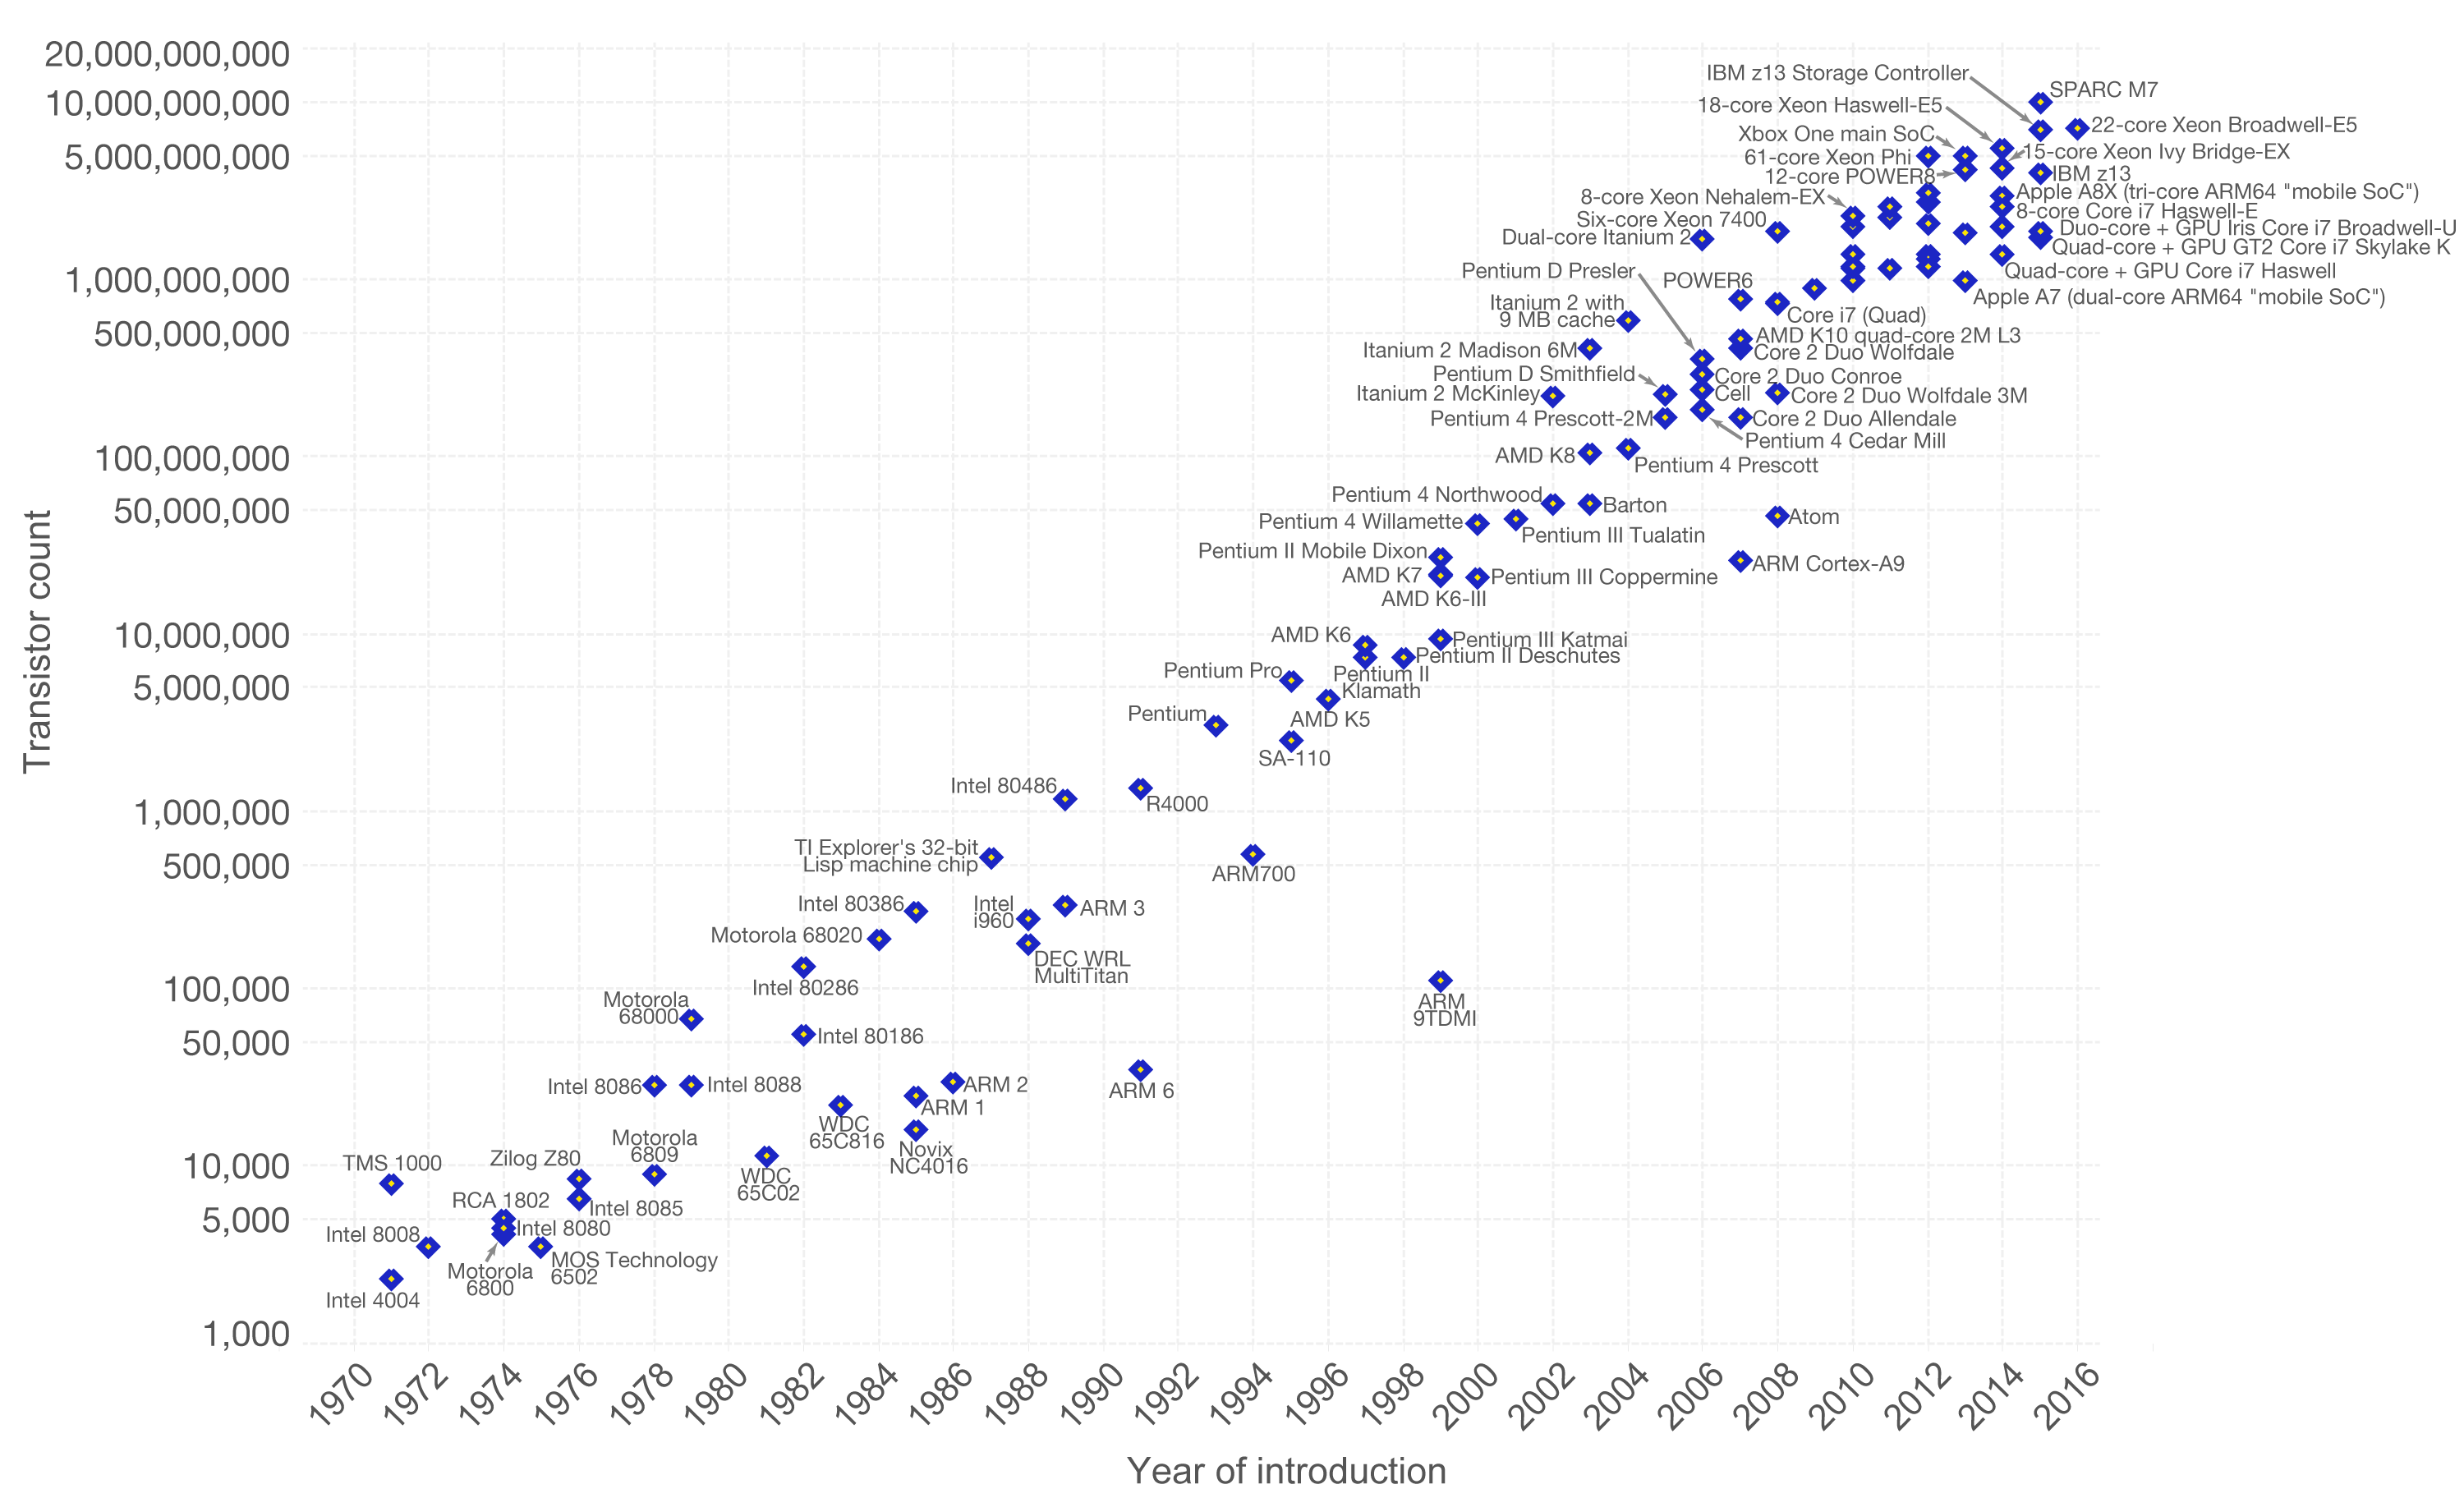
\includegraphics[width=1.2\textwidth]{./images/parallel_programming/moore_law2}
\caption[Moore's Law regarding CPUs transistors number.]{Moore's Law regarding CPU transistors number. \textsc{Intel} co-founder, Gordon Moore in 1695 observed that number of transistors in integrated circuits doubled each year. Although the pace has slowed in recent times, the number of transistors per square centimeter has since doubled approximately every 18 months. This is used as the current definition of the law. It is expected to hold true until 2020-2025. Note the logarithmic vertical scale. The almost linear trend correspond to an exponential growth.
}
\label{fig:moore}
\end{figure}
At same point the gain in performance in terms of clock speeds fails to increase proportionally with the additional efforts needed to overcome heat dissipation problems that in turn, become more and more important and challenging.
The heat emitted from the modern processor, measured in power density rivals the heat of a nuclear reactor core (see Figures \ref{fig:tempCPU} and \ref{fig:tempCPU_thermal})!
Additionally, the transistor resolution on the wafer is not far from from its physical limit (at the atomic scale), preventing further improvements.
But the power demand did not stop in these year, and is not going to stop in the near future, and from these reason comes the necessity of relying heavily on parallel architectures.
Today, the dominating trend in commodity CPU architectures is multiple processing cores mounted on a single die operating at "reduced" clock speeds  sharing resources and memory with each other.
Multi-core (2,4,8,12, up to 40) CPUs on a desktop PC at home or at the office are ubiquitous at the point that is even hard to be able to buy a single core device.
Even smart-phones are proper multi-core machines; for instance, the popular mobile CPU, the \textit{Snapdragon 835}, manufactured by \textit{Qualcomm} is a $8 \times$ cores, each of them with a clock speed up to $2.45$ \si{GHz}.
\begin{figure}[!htbp]
\centering
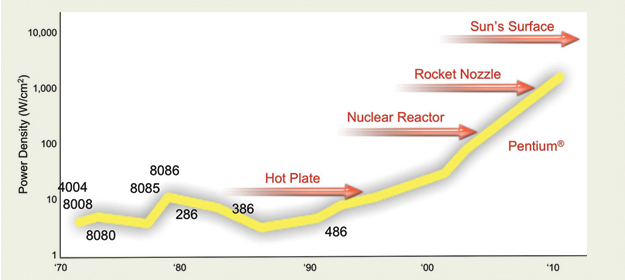
\includegraphics[width=1.0\textwidth]{./images/parallel_programming/temperatureCPU}
\caption[Temperature density of CPUs over the years.]{Integraed Circuits power density over the years. Note  that since 2000s power density is higher in CPUs than in nuclear reactors. This clearly shows that this trend is not sustainable.}
\label{fig:tempCPU}
\end{figure}
Lot of efforts have been put during these years in order to mitigate and overcome the limits that the sequential computer architecture has which its three main components impose:
\begin{enumerate}
\item Processor (Cores, branch prediction etc.)
\item Memory (Ram, Caches, Registers etc.)
\item Communication system i.e. datapaths,usually buses (PCI or SCSI)
\end{enumerate}
All three components present bottlenecks that limit the overall computing performance capability of a system.
Caches, low-latency high bandwidth and small capacity high speed memories, for example can hide latency of DRAM storing the fetched data and serving subsequent requests of the same memory (or neighboring) locations\footnote{The fraction of the data served by the various caches is commonly refeered to as \textit{\textbf{hit rate}}.}.
But one of the most important innovation that addresses these bottlenecks is \textbf{multiplicity} (in processors, memories and datapaths) that allows to improve the overall performance of a system and thus extending the size of the problems that a computer can solve.
Hardware multiplicity has been organized in several manners during the years, giving birth to a variety of parallel computer architectures.
\begin{figure}[!htbp]
	\centering
	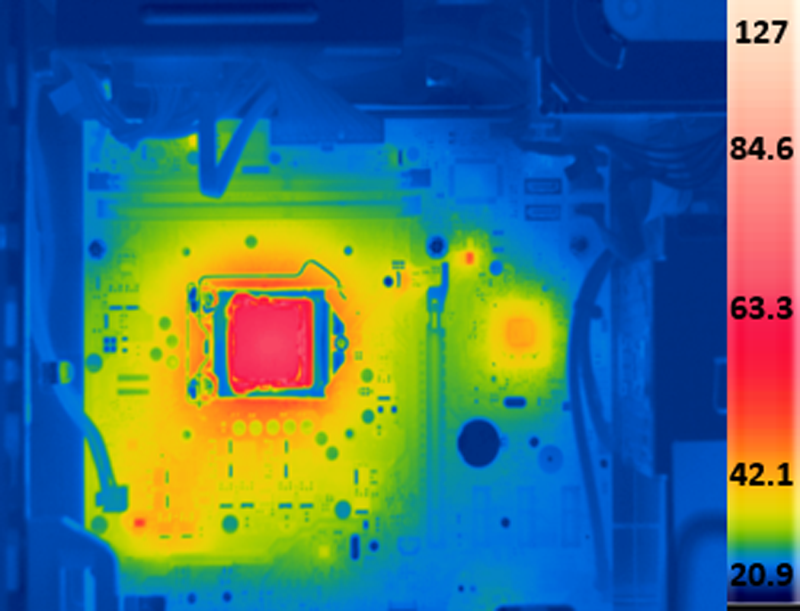
\includegraphics[width=0.5\textwidth]{./images/parallel_programming/heat_cpu}
	\caption[CPU and Motherboard Temperature.]{Thermal camera image of a modern CPU showing that the whole CPU heat is concentrated in a small part of the wafer i.e. power density is. is very high in some areas.}\label{fig:tempCPU_thermal}
\end{figure}

\section{Parallel Architectures - Flynn's taxonomy}
\label{sec:flynn_tax}
A number of definitions and classifications have been proposed  over the years in order to categorize parallel systems, the majority of them are mostly based on the adopted hardware configuration or on the logical approach in handling and implementing the parallelism.
Among all, \textit{Flynn}'s  taxonomy \cite{flynn:1972,duncan:1990} is probably the most famous and it is also well accepted by the scientific community, therefore introduced briefly in this section.

Flynn's classification is based on the notion of  \textit{stream of information}.
Two types of information flow into the processor: \textbf{instructions} and \textbf{data}.
Conceptually they can be separated into two independent streams.
A coarse classification can be made taking in account only the number of streams of both instructions and
data that an architecture can manage concurrently (see figure \ref{fig:parallelClassification1}).
Flynn's taxonomy classifies machines according to whether they have one or more streams of each type.
\begin{table}
		\caption[Flynn's Parallel architecture taxonomy]{Flynn's Parallel architecture taxonomy.}
	\label{fig:parallelClassification1}
	\begin{tabular}{lcccc}\toprule
		&\multicolumn{2}{c}{\textbf{\textsf{Single Instruction}}}&\multicolumn{2}{c}{\textbf{\textsf{Multiple Instructions}}}
		\\\cmidrule(r){2-3}\cmidrule(r){4-5}   
		&\textbf{\textsf{Single Data}}&\textbf{\textsf{Multiple Data}}&\textbf{\textsf{Single Data}}&\textbf{\textsf{Multiple Data}}\\\midrule
		& \textsc{sisd} & \textsc{misd}
		& \textsc{misd} & \textsc{mimd}
		\\\bottomrule
	\end{tabular}

\end{table}
Flynn's classifies architectures into four main categories:
\begin{description}
\item[SISD:] \textit{\textbf{Single}} instruction \textit{\textbf{Single}}
data.\hfill\\
No parallelism in either instruction or data streams.
Each arithmetic instruction initiates an operation on a data item taken from a single stream of data elements.
A single control unit fetches a single instruction from the memory.
Mainframes belong to this category.
\item[SIMD:] \textit{\textbf{Single}} instruction \textit{\textbf{Multiple}} data. \hfill \\ 
Data parallelism. The same instruction is executed on a batch of different data.
The control unit is responsible for fetching and interpreting one instruction at a time.
When it encounters an arithmetic or an other data ALU instruction, it broadcasts the instruction
to all processing elements (PE), which then all perform the same operation in unison.
For example, the instruction might be \texttt{add R3,R0.}.
Each PE would add the contents of its own internal register R3 to its own R0.
This is how stream processors work, for example, data elements are distributed across all available data memories. and the same instruction executed on each PE.
\texttt{SSE} and \texttt{AVX} extensions to the $x86$ processors family is an example of such parallelism.
One single instruction can operate on up to $512$ byte of data (see Figure \ref{fig:SSEvectorization} and Listing \ref{code:avxvectorization}).
SIMD exploits \textbf{data and spatial parallelism} in a synchronous manner.
\lstset{language=[OpenCL]C,frame=tb,
	caption=[Multiplying eight floats using Intel AVX vectorization.]{Multiplying eight floats of one array by eight floats of a second array and add the result to a third array. Serial and SIMD (AVX2) code examples. Note that the AVX2 intrinsic function \texttt{\_\_mm256\_fmadd\_ps} processes twentyfour floats, but it does not map to a single instruction (see Figure \ref{fig:SSEvectorization}). Instead, it executes three instructions: \texttt{vfmadd132ps}, \texttt{vfmadd213ps}, and \texttt{vfmadd231ps}. Despite this, it executes quickly and it is much faster than looping through the individual elements.}, 
	label=code:avxvectorization, 
	basicstyle=\footnotesize\ttfamily,
	keywordstyle=\color{ultramarine}\ttfamily,
	stringstyle=\color{rosemadder}\ttfamily,
	commentstyle=\color{gray}\ttfamily,
	backgroundcolor=\color{gray!5}, 
	numbers=left,numbersep=3pt,, 
	numberstyle=\tiny\ttfamily\color{gray},
	morekeywords=[2]{__m256,_mm256_fmadd_ps},
	%keywordstyle=[2]\color{violet},
}
\begin{lstlisting}
//adds 8 floats in a serial fashion. One at the time in 8 different steps
void multiply_and_add(const float* a, const float* b, const float* c, float* d) {  
	for(int i=0; i<8; i++) {
		d[i] = a[i] * b[i];
		d[i] = d[i] + c[i];
	}
}
//A single instruction adds 8 floats in a SIMD fashion
__m256 multiply_and_add(__m256 a, __m256 b, __m256 c) {
	return _mm256_fmadd_ps(a, b, c);
}
\end{lstlisting}
\begin{figure}[!htbp]
	\centering
	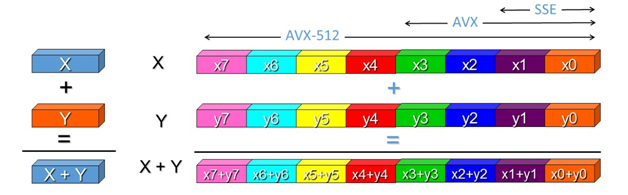
\includegraphics[width=1.0\textwidth]{./images/parallel_programming/vectorization_example}
	\caption{Example of vectorization with Intel SSE and extension.}
	\label{fig:SSEvectorization}
\end{figure}

\item[MISD:] \textit{\textbf{Multiple}} instruction \textit{\textbf{Single}} data. \hfill \\ 
Multiple instruction operating on the same single data stream  (ee Figure \ref{fig:MISD}). It is a class of system very unusual. No machines in this category have been commercially successful or had any impact on computational science. 
A type of computer  that fits the MISD description is the so called \textit{systolic array} \cite{fortes:1987,kung:1984} which consists of a network of pipelined primitive computing nodes or processors. 
\begin{figure}[!htbp]
	\centering
	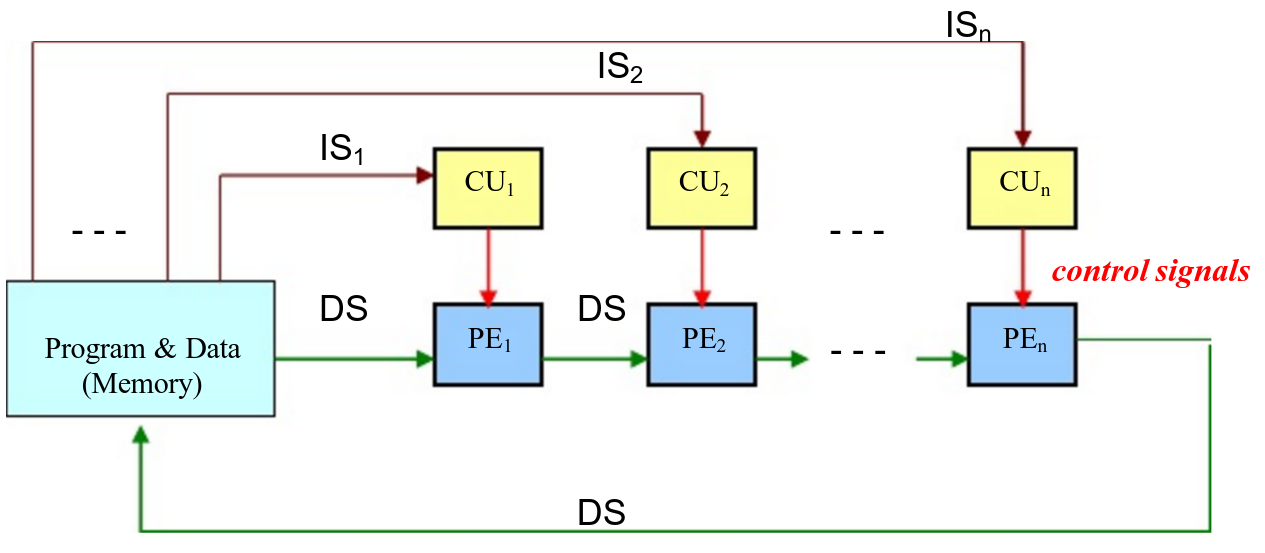
\includegraphics[width=1.0\textwidth]{./images/parallel_programming/MISD}
	\caption{MISD machine schematization. Each processor $CU_i$ has its own instruction flow and all operates on the same data.}
	\label{fig:MISD}
\end{figure}
 
\item[MIMD:] \textit{\textbf{Multiple}} instruction \textit{\textbf{Multiple}} data. \hfill \\
Multiple instructions operating independently on multiple data streams.
Most modern computers belogn to this family. A MIMD machine is an example of a true multiprocessor and are often employed to perform the so called \textit{Single Program Multiple Data} computation where each independent processor executes the same program.
Note that modern machine also exposes SIMD capability within each instruction stream.
MIMD architecture can be further divided by considering the  layout organization of memories:
\begin{description}
	\item [Shared Memory (modern CPUs)] where each processors shares the same memory address space and are interconnected by shared buses. 
	Shared memory architecture are usually shipped as \textit{Symmetric Multi Processors} (SMP) since each of them is usually identical in computational and access to resources capabilities, and the OS kernel can run on any of them in contrast to \textit{Asymmetric Multiprocessor}s where there is a master-slave relationship  among the group of processors.
	According to whether subsets of processors have a dedicated/private memory module we can categorize SM architectures in:	
	\begin{itemize}
		\item UMA (Uniform Memory Access) : Identical processors with equal
		access time to memory (see figure \ref{fig:UMA_NUMA}).
		Also known as \textit{Cache Coherent UMA} (CC-UMA), because the
		hardware ensures that all the processor can see a modification in memory performed by one of them.
		\item NUMA (Non Uniform Memory Access): Usually different groups
		 Symmetric multiprocessors (SMP), group of usually not more than 32 processors communicating via buses, are inter-connected, and processors belonging to different SMP can access the memory spaces of each others. Time for memory access is not uniform because the cost for a communication among SMP is higher than a intra-SMP one.
		 As for UMA, if a cache coherence mechanism  is present, then this architecture is called \textit{CC-NUMA}.
		 \begin{figure}[b]
			\caption[Shared memory architectures.]{UMA and NUMA shared memory architecture.}
			\label{fig:UMA_NUMA}
			\centering
			\begin{subfigure}[b]{0.5\textwidth}
				\centering
				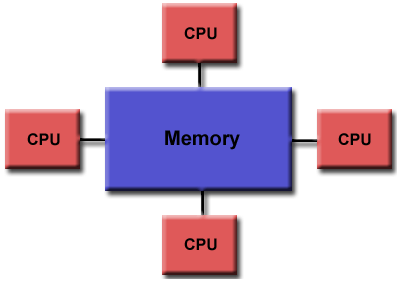
\includegraphics[width=0.92\textwidth]{./images/parallel_programming/shared_mem}
				\caption[]{}%
			\end{subfigure}%
			\begin{subfigure}[b]{0.5\textwidth}
				\centering
				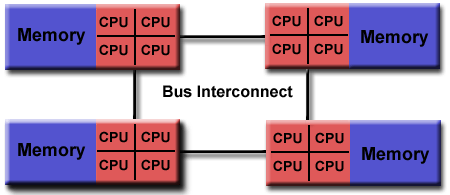
\includegraphics[width=0.92\textwidth]{./images/parallel_programming/numa}
				\caption[]{}%
			\end{subfigure}%

		\end{figure}
	\end{itemize}
	SM architecture provides an easy perspective to memory,	data sharing across processors and parallelism since no explicit communication is involved. Memory accesses and communications are fast due to the proximity of memory to CPUs, but it is not scalable because adding more CPUs to the pool can geometrically increases the traffic on the bus and makes cache management harder. Additionally, ensuring the correctness of accesses to global memory, in order to avoid race-conditions, is up to the programmer.
	As an example of real world SM modern processor, Figure \ref{fig:intelPhi} shows the Intel \textit{Knights Landing} architecture for the Intel Phi processor family which is armed with 72 cores, $8$ billions transistors at \SI{14}{\nano\metre}, AVX-512 and is able to executes 240 threads simultaneously.
	Coupled with this architecture many software model can be used to program
	SM machines. Among all, the most used are:
	\begin{itemize}
		\item Threads; Lightweight processes but with same PID (e.g. pthreads)
		\item Compiler preprocessor directives; A standard language with preprocessor directives to the compiler that is capable of converting the serial program in a parallel one without any (or very few) interventions or hints by the programmer (e.g. \texttt{OpenMP}, introduced in Section \ref{sec:openmp}).		
	\end{itemize}	
	\item [Distributed Memory] 	Different systems, and hence, different multiprocessors connected via some kind of network (see Figure \ref{fig:distribuiteMemory}), usually high speed networks such as gigabit \textsc{Ethernet} \cite{Spurgeon:2000:EDG:336070}, \textsc{InfiniBand} \cite{Shanley:2002:INF:579371} and \textsc{Myrinet} \cite{Boden:1995:MGL:623261.623898}, where the memory space in one processor does not map to another's one.
	Each of them operate independently on its memory address, so changes are not reflected on memory spaces of the others. Explicit communication is required between processors with synchronization under the programmer responsibility.
	This architecture  is very scalable and there is not  overhead in maintaining	cache coherency. 	
	The most used paradigm for programming distributed memory machines is the
	message passing for which the \textit{Message Passing Interface} (\texttt{MPI}\footnote{\url{http://www.mpi-forum.org/}}) \cite{Forum:1994:MMI:898758,Gropp:1999:UMA:555151} is the \textit{de facto} industrial and academic standard.
	
	\item[Hybrid Systems] As the name suggest a system belonging to this category, is a mix of architectures. Only a limited number of  processors, say $N$, have access to a common amount of shared memory. They are  inter-connected to the others groups via network. Each group  usually is an agglomerate of many computing cores (SMP).
		Hybrid systems of the kind described in this section are usually programmed using a combination of the message passing model (\texttt{MPI}) with the threads model (\texttt{OpenMP}) in which:
		\begin{itemize}
			\item threads perform computationally intensive task, using local
			\textbf{on-node} memory space, taking advantage of spatial locality of data (via vectorization/AVX for instance) and 
			\item communications between processes on different nodes occurs over network using \texttt{MPI} (see figure \ref{fig:hybridMemory}).
	\end{itemize} 
\end{description}
 
 \begin{figure}
 	\centering
 	\begin{subfigure}{0.55\textwidth}
 		\centering
 			\caption{Hybrid memory architecture (each processor is milti-core)}
 		\label{fig:hybridMemory}
 		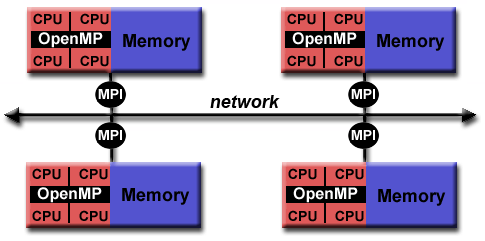
\includegraphics[width=0.95\textwidth]{./images/parallel_programming/hybrid_model}
 	
 	\end{subfigure}%
 	\begin{subfigure}{0.45\textwidth}
 		\centering
 		\caption{Distributed memory architecture.}
 		\label{fig:distribuiteMemory}
 		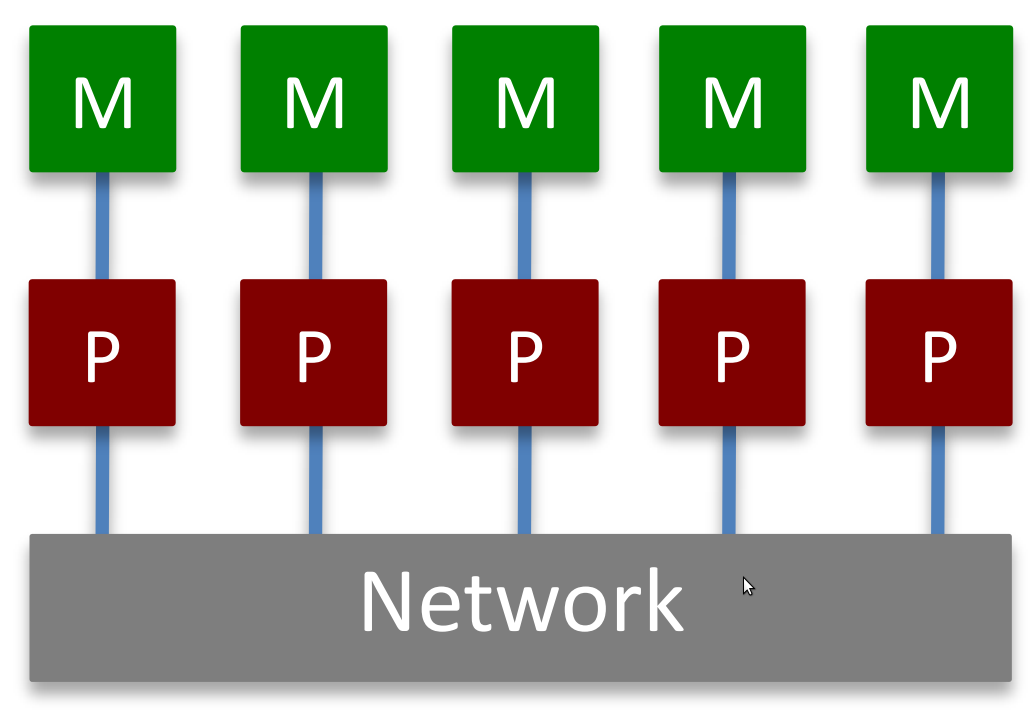
\includegraphics[width=0.92\textwidth]{./images/parallel_programming/distribuitedMemory}
 	\end{subfigure}%
 \end{figure}

\begin{figure}
	\centering
	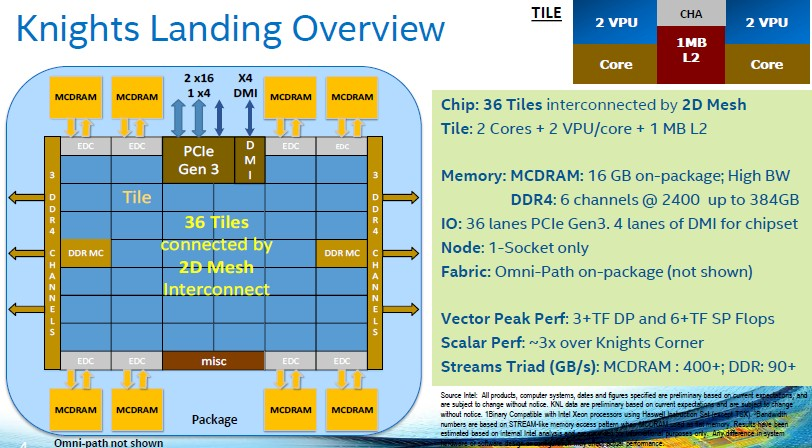
\includegraphics[width=1.0\textwidth]{./images/parallel_programming/xeonphi}
	\caption{Xeon Phi, Intel Knight Landing architecture and technical specifications.}
	\label{fig:intelPhi}
\end{figure}



\section{The \texttt{OpenMP} Parallel Computing Paradigm for Shared Memory Computers}
\label{sec:openmp}
    \texttt{OpenMP} is a portable API providing compiler directives and library
    functions for shared memory parallel programming in \texttt{C/C++} and
    Fortran \cite{Chapman:2007:UOP:1370966} designed on top of \texttt{pthread} \cite{Nichols:1996:PP:237813}. It implements the
    multi-threaded \emph{fork-join}  programming model (see Figure \ref{fig:omp_fork-join}), where an initial (or master) thread forks a given number of new threads (team of threads), which share the resources of the parent process and run concurrently on the available processing cores.
    Threads created during the \textit{fork} phase can therefore
    rejoin to the master thread (join phase), and more \textit{fork-join}
    stages can occur in a typical execution of an \texttt{OpenMP} executable.
    The size of the teams can be controlled by an environment variable \texttt{OMP\_NUM\_THREADS}, set at runtime by using the \texttt{omp\_set\_num\_threads(n)} function or specified for each parallel region using \texttt{num\_thread(n)} in the \texttt{\#pragma omp parallel} directive (see Listing \ref{code:openmp_lock}).
\begin{figure}[H]
	\centering
	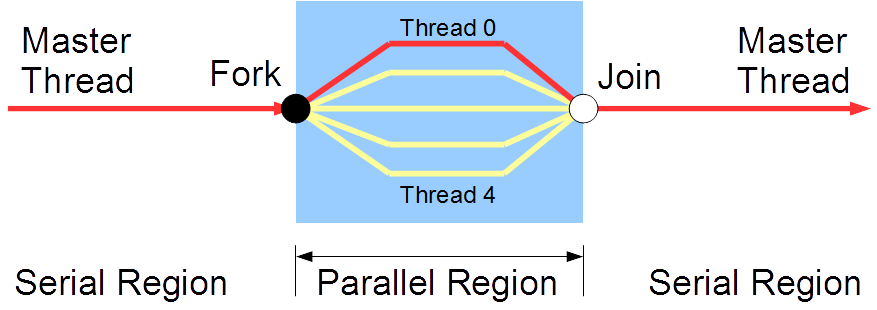
\includegraphics[scale=0.8]{./images/parallel_programming/omp_fork-join}
	\caption[\texttt{OpenMP} fork-join execution model.]
	{\texttt{OpenMP} fork-join execution model.
		\begin{inparaenum}
			\item OpenMP programs start with a single thread; the \textit{master thread} (\textit{Thread \#}$0$).
			\item At the starting point of a parallel region, \textit{master} creates team of parallel worker threads (\textbf{FORK}).
			\item Statements in the parallel block are executed in concurrently by every thread (master as well). 
			\item At end of parallel region, all threads \textbf{synchronize}, and join \textit{master} thread (\textbf{JOIN}).
		\end{inparaenum} Note that parallel regions can be nested.}
	\label{fig:omp_fork-join}
\end{figure}
    The \textit{fork-join} model allows for the selective parallelization of
    the original source code (e.g. loops), by leaving portions that
    are difficult to be parallelized or that would lead to negligible
    (or even worsening) improvements, unchanged with respect to the
    serial implementation.
    Numerical applications usually accomplish most of their work in a relatively small portion of their codebase, known as \textit{hotspots}. Those are the solely parts of an application that are worth parallelizing. Profilers and performance analysis tools are funamental and employed extensively during in order to identify such hotspots.   
    OpenMP can therefore effectively utilized to share the iterations of a loop within a pool of threads.
    
    By default, static scheduling is adopted where iterations are equally
    subdivided in chunks and statically allotted to threads in a
    round-robin policy. However, iterations can also be assigned to
    threads on demand, by using the \textit{dynamic} scheduling clause. In this
    manner, when a thread terminates processing its current chunk, it requests for a new one, usually resulting in better performance in the case where load is not well balanced across chunks.
    Scheduling can be specified using the \texttt{schedule} keyword in the \texttt{\#pragma omp for} directive.
    Static scheduling can be non-optimal in the case when different iteration take different amount of time to be executed. As an example consider the program in Listing \ref{code:scheduling_omp} in which each loop iteration causes the executing thread to sleep for a number of seconds equals to the number of the iteration. 
    \lstset{language=[OpenCL]C,
    	caption={Scheduling in OpenMP example. Note that specifying \textbf{static scheduling } is not needed since it is the default setting.}, 
    	label={code:scheduling_omp}, 
    	basicstyle=\ttfamily,
    	keywordstyle=\color{ultramarine}\ttfamily,
    	stringstyle=\color{rosemadder}\ttfamily,
    	commentstyle=\color{outerspace}\ttfamily,
    	backgroundcolor=\color{gray!5}, 
    	numbers=left, 
    	numberstyle=\tiny,
    	morekeywords=[2]{schedule,parallel,omp,pragma,num_threads,omp_get_thread_num,omp_destroy_lock,omp_unset_lock,omp_set_lock,omp_lock_t,omp_init_lock},
    	%keywordstyle=[2]\color{ultramarineblue}\ttfamily   	
    }
    \begin{lstlisting}
    #define CHUNK_SIZE (1)
    int main ( ) {
    	#pragma omp parallel for schedule(static,CHUNK_SIZE) num_threads(4)
    	for (int i = 0; i < N; i++) {
    		/* wait for i seconds */
    		sleep(i);    		
    		printf("Thread %d has completed iteration %d.\n", 
    				omp_get_thread_num( ), i);
    	}
    	/* all threads done */
    	printf("All done!\n");
    	return 0;
    }
\end{lstlisting}
Among the threads spawned by code in Listing \ref{code:scheduling_omp}, there is a great imbalance  in the number of seconds they will wait,  because the last thread executes the last chunk of iterations (which translates to longer sleep time).
\textit{Dynamic} scheduling can be applied in a case like this to improve the overall execution time. \texttt{OpenMP} assigns one iteration to each thread and when a thread completes its work, it is assigned the next iteration that has not been executed yet reducing execution time effectively. See table \ref{tab:scheduling_policies} for a complete list description of all kind of scheduling in OpenMP.

Moreover, \texttt{OpenMP} provides locking mechanism to serialize the access to shared variables by defining critical sections.
A lock must be firstly  initialized and then can be acquired or released.
When a thread  attempts to acquire a lock that is already be set by another
thread, its execution is suspended until the lock is released,
giving rise to performance degradation (or even to possible deadlock situations). 
However, a lock can also be queried in order to evaluate its state, without blocking the thread execution.
In thisway, if the lock is already set, the querying thread can do
perform other trasks, thus minimizing idle time.
See Listing \ref{code:openmp_lock} for an example of lock usage in OpenMP.
\begin{minipage}{1.0\textwidth}
\lstset{language=[OpenCL]C,
	caption={\texttt{OpenMP} lock acquisition, usage and destruction example. Note that the region of code between lines 6 and 8 is serialized.}, 
	label={code:openmp_lock}, 
	basicstyle=\ttfamily,
	keywordstyle=\color{ultramarine}\ttfamily,
	stringstyle=\color{rosemadder}\ttfamily,
	commentstyle=\color{outerspace}\ttfamily,
	backgroundcolor=\color{gray!5}, 
	numbers=left, 
	numberstyle=\tiny,
	morekeywords={#pragma,omp_destroy_lock,omp_unset_lock,omp_set_lock,omp_lock_t,omp_init_lock}
}
\begin{lstlisting}
omp_lock_t writelock;
omp_init_lock(&writelock);
#pragma omp parallel for num_threads(5)
for ( i = 0; i < x; i++ ){
// some stuff in a concurrent fashion
omp_set_lock(&writelock);
// one thread at a time stuff
omp_unset_lock(&writelock);
// some more  stuff in a concurrent fashion
}    
omp_destroy_lock(&writelock);
\end{lstlisting}
\end{minipage}   

    In addition to the data-type parallelization provided by the
    fork-join model, \texttt{OpenMP} aslo supports the functional-type
    parallelization, where different portions (called \textit{regions}) of code to be
    processed are assigned to different threads. In both cases, \texttt{OpenMP}
    parallelization of a code is straightforward, by hiding most
    low-level implementation details.
    Moreover, by using \texttt{OpenMP} it is
    possible to build the same source code to produce both parallel or
    sequential executable. In the latter case, the compiler simply
    ignores the \texttt{\#pragma omp} directives.
    \begin{table}
    	   	\begin{tabularx}{1.0\textwidth}{cX}
    		\rowcolor{gray!35}	
    		\heading{\textbf{Scheduling Kind}} &  \heading{\textbf{Description}} \\ \hline
    		\rowcolor{gray!15}
    		\texttt{\textbf{static}} & The loop is divided into equal-sized chunks of iterations. By default, chunk size is $\frac{iterations}{number\_of\_threads}$. If the chunk size is set to $1$, iteration are executed by the threads in a interleaved fashion.\\ \hline
    		\rowcolor{gray!5}
    		\texttt{\textbf{dynamic}} & chunk-sized block of iterations are internally queued. When a thread is ready to execute some work, it retrieves the next block  from the top of the queue. Note that by default chunk size is $1$. Managing the queue and assigning work to  to threads comes with an arrached overhead.\\ \hline
    		
    		\rowcolor{gray!15}
    		\texttt{\textbf{guided}} & similar execution policy  to \texttt{dynamic} but che chunk size decreases over time to better handle load imbalance between iterations. In this cake the optional parameter of the schedule construct specifies the minimum chunk size. By default it is equal to $\frac{iterations}{number\_of\_threads}$\\ \hline
    		
    		\rowcolor{gray!5}
    		\texttt{\textbf{auto}} & The compiler is free to decide any possible mapping of iteration to threads.\\ \hline
    		
    		\rowcolor{gray!15}
    		\texttt{\textbf{runtime}} & the scheduling policy is choosen at runtime and changes according to the environment variable \verb|OMP_schedule| \\ \hline
    	\end{tabularx}
    
    	\caption[OpenMP scheduling policies]{\texttt{\#pragma omp parallel for schedule(kind [,chunk size])} OpenMP scheduling kinds. The optional parameter (chunk size), when specified, must be a positive integer. }
    	\label{tab:scheduling_policies}
    \end{table}
    
    \subsection{General Purpouse GPU Computing - GPGPU}
    The concept of many processors working together in concert is not new in computer graphics. Since the demand generated by entertainment started to grow, multi-core hardware emerged in order to take advantage of the high amount of parallel work available in the process of generating and rendering and manipulation of $3D$ images.
    The main goal of the computer graphics is to render and then display $3D$ images onto the screen, which translates to refreshing pixels at rate of sixty or more $\si{Hz}$ \cite{Akenine-Moller:2002:RR:553838}.
    Each pixel has to be processed goes through a number of stages, and this process is commonly referred as to the \emph{graphic processing pipeline}.
    The peculiarity of this task is that the computation of each pixel is independent of the other's.
    This specific task is thus suitable for distribution over parallel processing elements as it can be categorized as  a \textbf{embarassingly, perfect} or \textbf{pleasingly} \textit{parallel} problem\cite{Foster:1995:DBP:527029} (see Section \ref{sec:opencal_julia} and Listing \ref{code:julia_set} at pages \pageref{sec:opencal_julia} and \pageref{code:julia_set} respectively, for an example of a perfectly parallel problem).
    To support extremely fast processing of large graphics data sets (which mainly consists of vertices and fragments), modern GPUs employ a stream processing model with parallelism.
    The game industry boosted the development of  GPUs, that offer today greater performance than CPUs and are improving faster too as shown in Figures  \ref{CPU-VS-GPU_GFLOP} and \ref{CPU-VS-GPU_MEMORY}.
    The reason behind the discrepancy in floating-point capabilities between CPU and  GPU is that GPUs are designed such that more transistors are devoted to data crunching and processing rather than caching, flow control, branch prediction, etc..
    Also note that memory bandwith is still one of the main advantages of GPU and Xeon Phi over CPUs architectures. The gap is getting wider thanks also to the introduction of High Bandwidth Memories (HBM), stacked memory by NVIDIA and MCDRAM for Xeon Phi \cite{Sodani:7477467,Jun:7939084}. 
    \begin{figure}[!htbp]
    	\centering
    	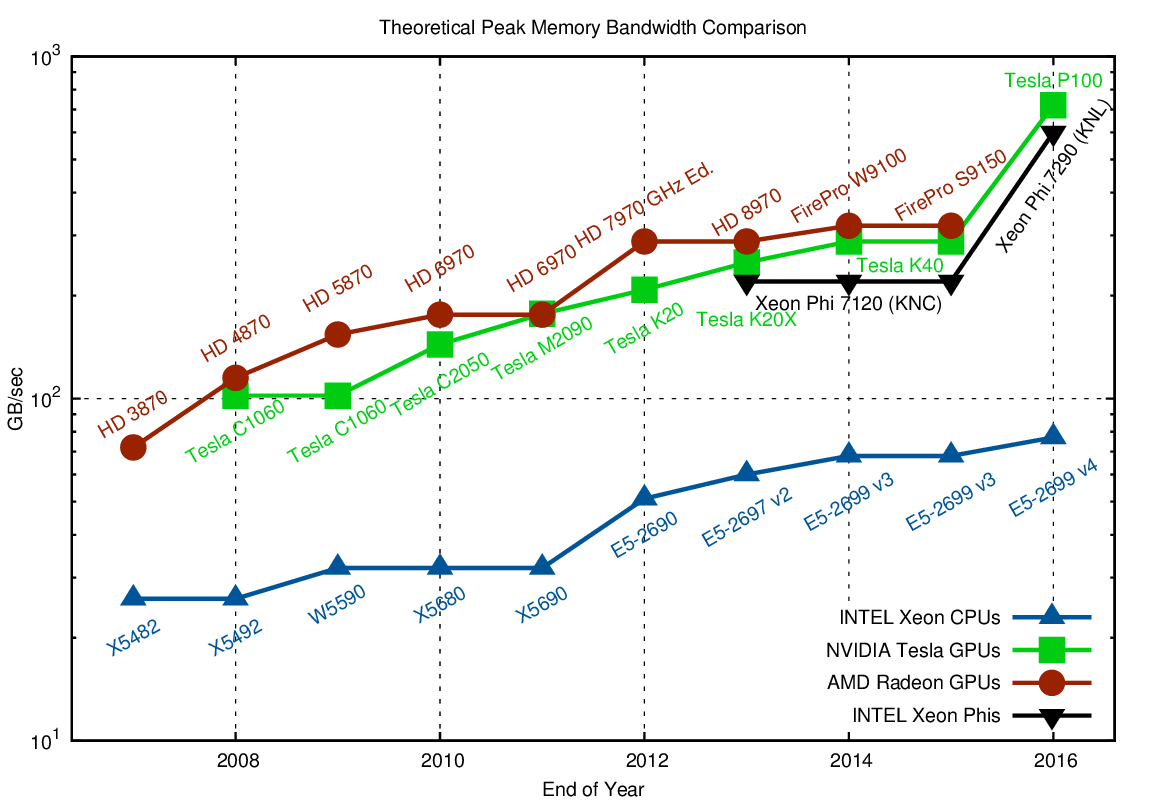
\includegraphics[width=1.0\textwidth]{./images/parallel_programming/memory-bandwidth}
    	\caption[\textsc{Intel} CPUs and \textsc{NVIDIA} GPUs memory bandwidth
    		chart]{Memory Bandwidth comparisong between \textsc{Intel} CPUs and \textsc{NVIDIA} chips over time. Higher is better.}
    		\label{CPU-VS-GPU_MEMORY}
    \end{figure}
    \begin{figure}[!htbp]
    	\centering
    	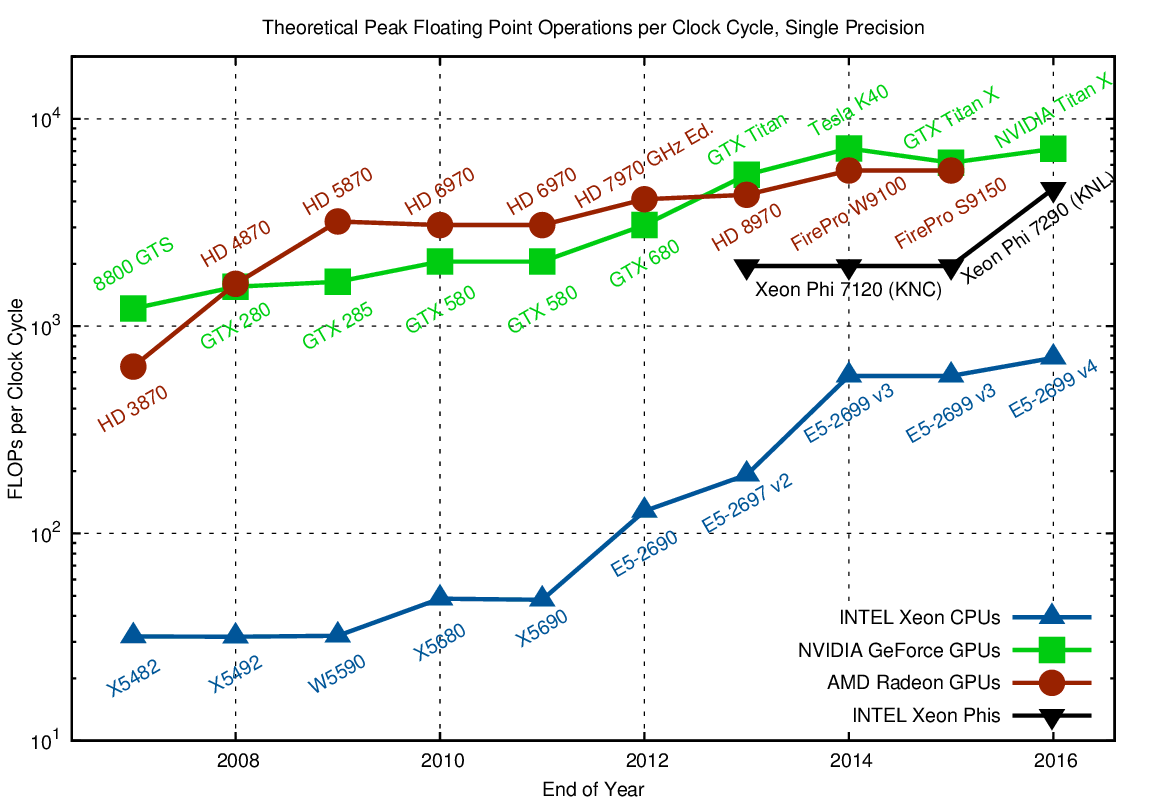
\includegraphics[width=1.0\textwidth]{./images/parallel_programming/cpu-vs-gpu}
    	\caption[Performance comparison (FLOPs) between CPU and modern accelerators (\textsc{NVIDIA}, \textsc{Intel} and \textsc{AMD})]{Performance comparison (FLOPs) between CPU and modern accelerators (\textsc{NVIDIA}, \textsc{Intel} and \textsc{AMD}) over time. When Double precision is considered, relative performance between the considered hardware does not change. Higher is better.}\label{CPU-VS-GPU_GFLOP}
    \end{figure}
    Nowadays, GPU are widely used for general purpouse computing. The Top $500$ supercomputers  ranking \footnote{\url{http://www.top500.org/statistics/list/}}  \cite{Strohmaier:2006:TS:1188455.1188474} is dominated by massively parallel computer, built on top of superfast networks and millions of sequential CPUs working in concert.
    But as the industry is developing even more powerful, programmable and capable GPUs in term of \si{\giga FLOPS},  we see that they begin to offer advantages over traditional cluster of computers in terms of economicity and scalability as depicted in Figure \ref{gflops-per-watt-sp}.
        \begin{figure}[!htbp]
    	\centering
    	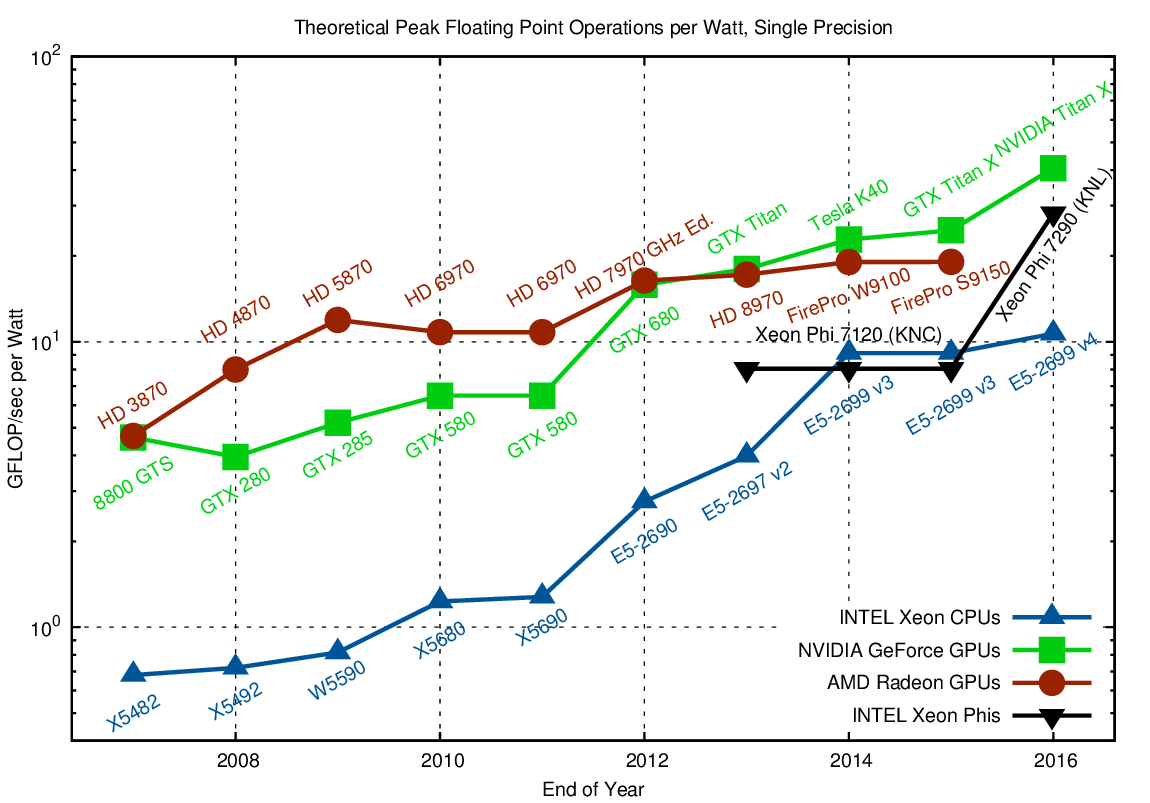
\includegraphics[width=1.0\textwidth]{./images/parallel_programming/gflops-per-watt-sp}
    	\caption[GFLOPs per \si{Watt} metric for CPUs and GPUs]{GFLOPs per \si{Watt}, Higher is better. GPUs offer higher performance per Watt utilised especially for those fine-grained massively parallel problems such as dense matrix-matrix multiplication. Note that the Figure also shows that the CPU is getting smaller, indicating that CPU are introducing more GPU-like capabilities into their transistors. \textit{Intel} added wider vector processing units (up to 64 byte) to their latest processors. }
    	\label{gflops-per-watt-sp}
    \end{figure}
  
    \subsection{From Graphics Graphics to General Purpose HW}\label{sec:graphicPipeline}
    A graphics task such as rendering a $3D$ scene on the screen
    involves a sequence of processing stages inside the GPU, i.e. shaders, that run in parallel and in a prefixed order, known as the graphics hardware
    pipeline \cite{Shirley:2005:FCG:1088893} which is the most common form of 3D computer rendering, distinct from, for instance, \textit{raytracing} or \textit{raycasting} for which the concept of pipeline is not even defined.
     \begin{figure}[H]
    	\centering
    	\caption{Typical computer graphics pipeline.}\label{fig:graphicPipeline}
    	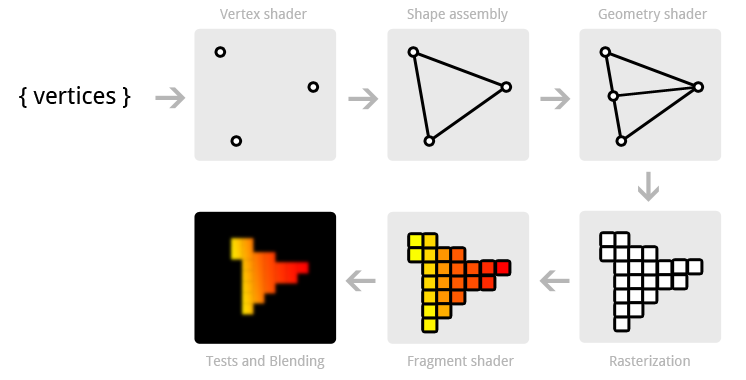
\includegraphics[width=1.0\textwidth]{./images/parallel_programming/pipeline}
    \end{figure}
    
     Figure \ref{fig:graphicPipeline} shows the important key steps that make up the graphic pipeline and for which the GPU hardware has been specialized for years. The pipeline works taking as input graphics primitives, each stage forward its results on to the next stage.
    \begin{itemize}
    	\item     The first stage of the pipeline is the \textit{vertex shader}. The
    	input to this phase is a list of vertices in object space coordinate which are then converted to world coordinates (applying the \textit{model and view matrices}).
    	\item  Shape assembly is performed where vertices are grouped together by forming graphics primitives, i.e. lines, point, polygons, triangles, tringles strips etc. If enabled, lighting calculation are also performed for each vertex.
    	\item   The following step, the \textit{geometry shader} is optional in the \texttt{openGL} pipeline and can be used to produce or delete primitives. One of the most common use of this shader is in reducing the communication between the GPU and the CPU. For instance one can only pass to the graphic pipeline a list of vertices for drawing cubes, and produce the primitives for them only when the the geometry shader is executed, reducing the amount of information exchanged between the CPU and the GPU.
    	\item   Each of the (from the now final list of) primitives is scan-converted or rasterized generating a set of fragments in screen space for the visible only part of the shapes. Each fragment stores the state information needed to update a pixel and are obtained by interpolating per vertex attributes coming from the geometry shader. For instance, each vertex of a triangle end up having its color changed based on the the color of its neighbors. 
    	\item  In the \textit{fragment  shader} is used to calculate the final color of each individual fragment. Texture coordinates of each fragment are used to fetch colors of the appropriate texels (texture pixels) from
    	one or more textures. Further interpolation may also be
    	performed to determine the ultimate color for the fragment.
    	\item Finally, various tests (e.g., \textit{depth} and \textit{alpha}, etc.) are conducted to determine whether or how the fragment should be used to update a pixel in the frame buffer.    
    	Each shader in the pipeline performs a basic but specialised operation on the
    	vertices as it passes. 
    \end{itemize}

    In a shader based architecture the individual shader processors exhibit very limited capabilities beyond their specific purpose.
    Before the advent of CUDA in 2006 most of the techniques for non-graphics
    computation on the GPU took advantages of the programmable fragment processing stage. The steps involved in mapping a computation on the GPU are
    as follows:
    \begin{enumerate}
    	\item The data are laid out as texel colors in textures;
    	\item  Each computation step is implemented with a
    	user-defined fragment program. The results are encoded as pixel colors and rendered into a  pixel-buffer (stored into GPU main memory, similar to a frame-buffer); 
    	\item Results that are
    	to be used in subsequent calculations are copied to textures for temporary storage and the process could start over again for another iteration.
    \end{enumerate} 
    
    The year 2006 marked a significant turning point in GPU architecture. The \texttt{G80}  was the first \textsc{NVIDIA} GPU to have a unified architecture whereby the different shader processors were  combined into unified stream processors (see Figures \ref{fig:volta_sm} and \ref{fig:volta_architecture} at pages \pageref{fig:volta_sm}  \pageref{fig:volta_architecture} respectively). The resulting stream processors had to be more complex so as to provide all of the functionality of the shader processors they replace. Although research had been carried out into general purpose programming
    for GPUs previously, this architectural change opened the door to a far wider range of  applications and practitioners.
    GPUs are nowadays, well suited for data-parallel problems because they are very effective at executing the same code on many data elements at the same time  in a \textit{Single Instruction, Multiple Threads} (SIMT) fashion or using a more general definition as \textit{Parallel Random-Access Machine in which each thread Can Read or Write a memory location} (\texttt{CRCW PRAM}).
    
    
\section{The OpenCL Parallel Computing Paradigm on Heterogeneous Devices}
    Released on December 2008 by the Kronos Group, \texttt{OpenCL} \cite{Gaster:2011:HCO:2046379,Stone:2010:OPP:622179.1803953,Munshi:2011:OPG:2049883} is an open standard for programming heterogeneous computers built from CPUs, GPUs and other processors. It allows to define the intended computation using the \textit{platform} abstraction. A platform is composed by an host and one or more compute devices. A C-like language is used to program and orchestrate the various components of the platform (see Figure \ref{fig:openCL_platform}).
    
    One of the advantages of \texttt{OpenCL} is that it is not restricted, as in the case of CUDA\cite{NvidiaprogGuide}, to the use of GPUs only but it takes each computing resource in the system as computational peer unit, interposing a uniform set of API between them and the programmer, easing the process of interfacing with them. Another big advantage is that it is  open, free, and cross-compatible across vendors since is supported by all major hardware producers.
    
    A typical \texttt{OpenCL} application is subdivided in two parts, one
    running on the CPU (\textit{host} application) and one or more running on a
    compliant device (\textit{device} application), where the actual parallel
    computation generally takes place. The host application defines
    the tasks to be executed in parallel. Each parallel task is
    implemented as an \texttt{OpenCL} \emph{kernel}, which is a special C
    function, which is compiled at runtime for each specifically for and deployed to a compliant device, or to different ones, for execution. The execution model is similar to the one of CUDA (CUDA and OpenCL share a similar programming model and underlying hardware architecture, even if a quite different terminology is adopted), where each kernel is executed by \textbf{threads}, the smallest execution entity, also called \textbf{work-items}, which are grouped into \textbf{work-groups}. A work-item is executed by one or more processing elements as part of a work-group executing on a compute unit. A work-item has to be considered a thread in terms of its control flow and memory model, but the hardward and the compiler can run multiple work-items on a single thread. As an example one can imagine that work-items computation can be carried out on lanes of a SSE vector. 
    A work-group is a collection of related work-items that execute on a single compute unit. A work group must map to a single compute unit (a core on a CPU, or using CUDA terminology a streaming multiprocessor). 
    Work-groups can sunchronize internally between work-items using local or global memory or barriers but they cannot synchronize with each other, making impossible building locking and synchronization primitives (among work-groups).
    The  locality of execution of work-items  leads to more efficient synchronization, and makes possible to have access to user managed local fast memories and caches (similar to CPU L1 caches) in order to makes communication fast.    
    A work-item is distinguished from other executions within the collection by its \textbf{global ID} and \textbf{local ID} (relative to the parent worl-group).
    
    Work-groups can:
    \begin{itemize}
		\item \textbf{Share data} between the work-group's work-items using local memory
		\item \textbf{Synchronize} between work-items using barriers and memory fences mechanism
		\item \textbf{Use special built-in functions} such as \texttt{work\_group\_copy}
    \end{itemize}

    \begin{figure}
	\centering
	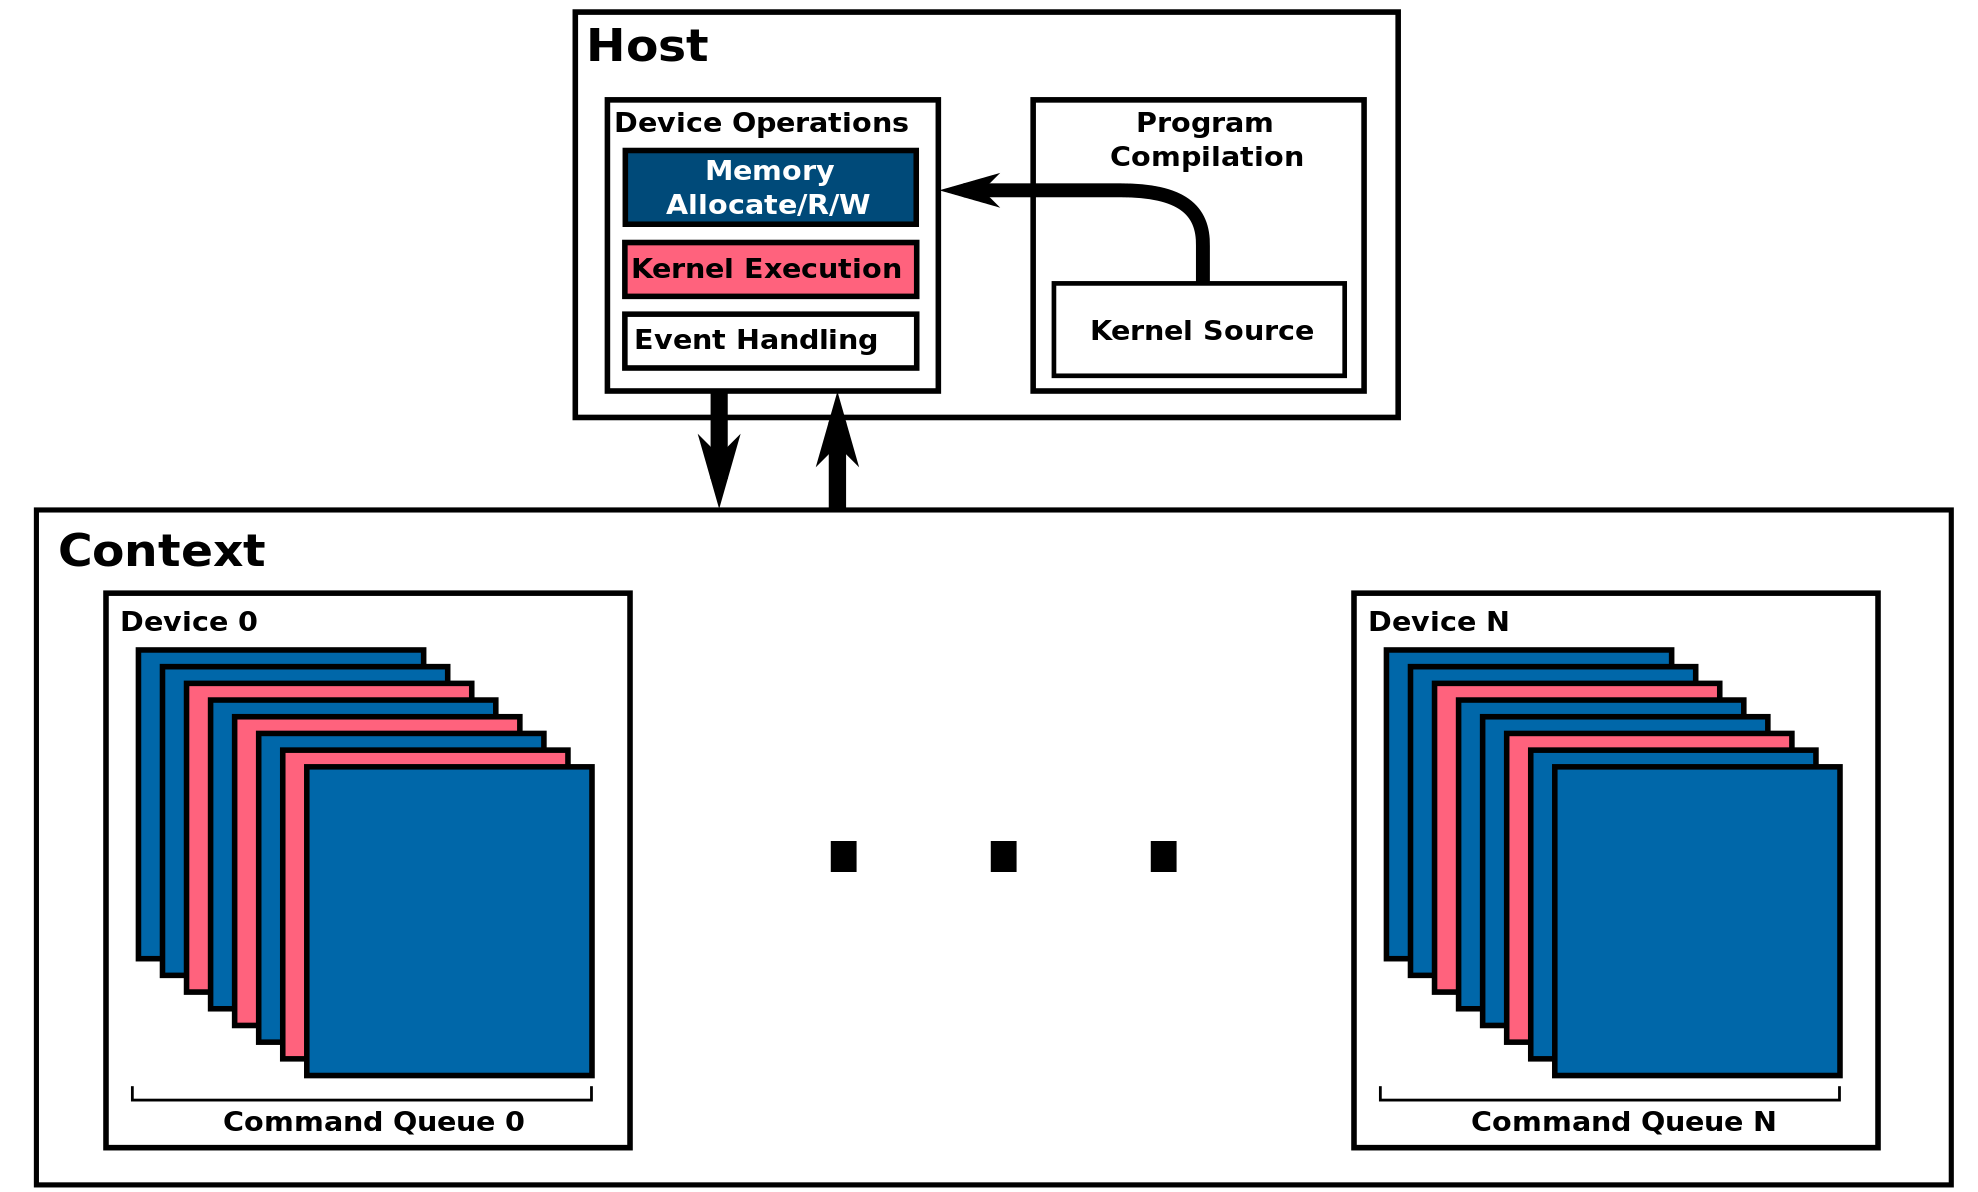
\includegraphics[width=1.0\textwidth]{./images/parallel_programming/openCL}
	\caption[\texttt{OpenCL} platform abstraction.]{\texttt{OpenCL} platform abstraction. A device is any supported device including GPU, CPU, FPGAs, etc.. Command queues are executed concurrently for each device and can be synchronized by means of API calls.}
	\label{fig:openCL_platform}
\end{figure}

    \begin{figure}
	\centering
	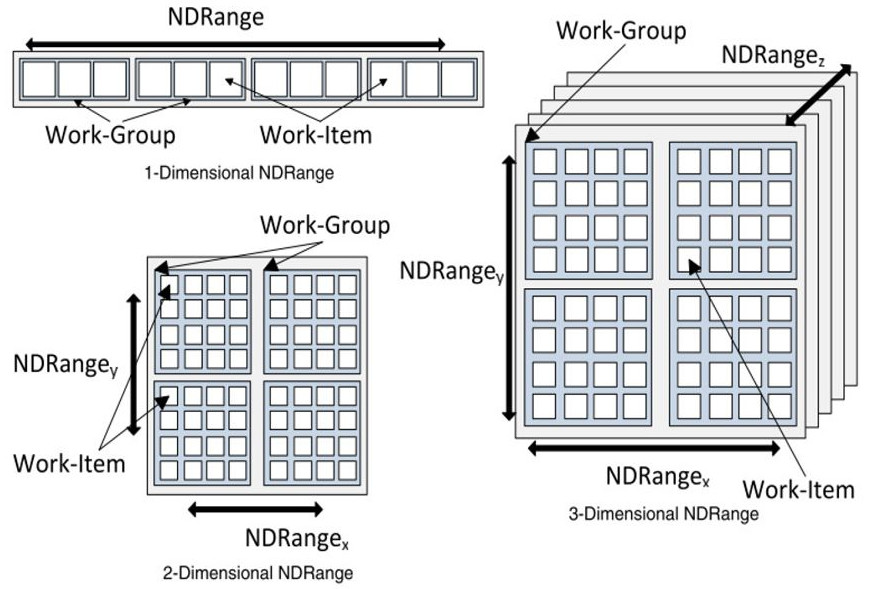
\includegraphics[width=0.85\textwidth]{./images/parallel_programming/opencl_execmodel}
	\caption{\texttt{OpenCL} 1D,2D,3D work-items and work-groups partitioning. }
	\label{fig:opencl_execmodel}
\end{figure}

	Work-groups and work-items are arranged in a indexed grid-like structure. 
    When launching the kernel for execution, the host code defines the grid dimensions, or the global work size. The host code can also define the partitioning to work-groups, or leave it to the implementation. During the execution, the implementation runs a single work item for each point on the grid (a kernel per work-item). It also groups the execution on compute units according to the work-group size. The order of execution of work items within a work-group, as well as the order of work-groups, is implementation-specific (see Figure \ref{fig:work_group_execution}).
    Data to be processed has to be explicitly partitioned and assigned to compute units because each work-item runs the same kernel on different portions of data in a \textit{SIMD/SIMT} fashion. For example, in case of an array of $n$ elements and $n$ work-items, data can be partitioned by associating each work item to the array element with index corresponding to the work-item global ID. Figure \ref{fig:opencl_execmodel} depicts how items and groups can be arranged when partitioned in $1D$, $2D$ and $3D$.
    Figure \ref{fig:opencl_execmodel2d} shows a $2D$ decomposition with details on global ID computation from local group and thread indices.
    
\begin{figure}[!htbp]
    	\centering
    	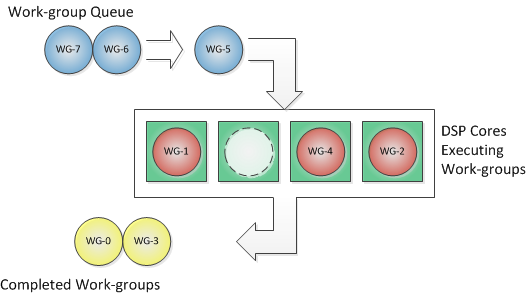
\includegraphics[width=0.85\textwidth]{./images/parallel_programming/work_group_execution.png}
    	\caption[\texttt{OpenCL} work group scheduling]{\texttt{OpenCL}  work-groups scheduling. 
    	The green boxes represent the computing unit. The circles represent the work-groups. Blue work-groups are waiting to be executed, pink work-groups are currently executing and yellow work-groups have been completed. Each work group is queued for execution and executes on a single computing unit (a GPU multiprocessor, CPU core, etc.) Note that execution order is not guaranteed by the standard.}
    	\label{fig:work_group_execution}
    \end{figure}

        \begin{figure}
    	\centering
    	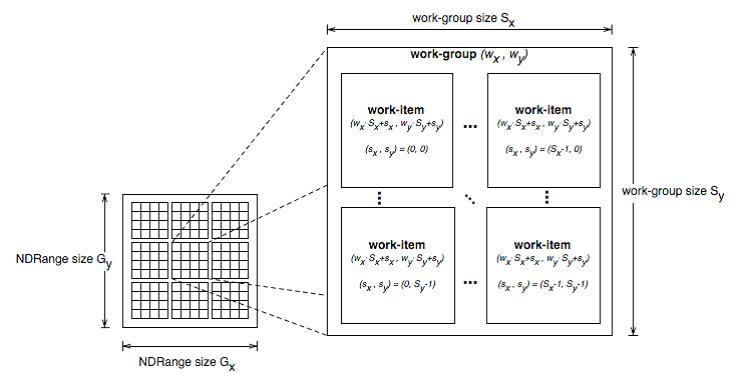
\includegraphics[width=1.1\textwidth]{./images/parallel_programming/opencl_execmodel2d}
    	\caption[\texttt{OpenCL} 2D work-items and work-groups detailed partitioning]{\texttt{OpenCL} 2D work-items and work-groups detailed partitioning. The computation of global index from local item and group index is also shown.}\label{fig:opencl_execmodel2d}
    \end{figure}
    When the kernel execution terminates,
    work-items globally synchronize, and the control returns to the
    host application. Similarly to the OpenMP fork-joins stages,
    different kernel executions and synchronization stages can take
    place in a typical \texttt{OpenCL} application.
    
    Data can be shared by all the running work-items by means of the
    device global memory, which is generally the largest among all the
    different memory levels available on the device (this is especially true for modern GPUs)
    though being the slowest. A read-only memory, equivalent to the
    global one in terms of latency and dimension, called constant
    memory, is also available. Some devices have an appropriate
    portion of this memory, while in other cases the constant memory
    space coincides with that of the global memory. Threads within a
    work-group are executed by a specific compute unit and therefore
    can share data on the local memory and also synchronize each
    other. Local memory is generally smaller with respect to the
    global one, but allows for faster access (about $100\times$ faster
    on modern GPUs). Eventually, each work-item has its own private
    memory, which is at the same time the fastest and the smallest
    one. 
    
    The memory in which a given data is stored must be
    initially defined and allocated by the host using the appropriate API calls (e.g. see Listing \ref{code:opencl_allocate}). 
    \lstset{language=[OpenCL]C,
    	basicstyle=\ttfamily,
    	caption={Allocate buffer API call in OpenCL.},
    	label={code:opencl_allocate},
    	morekeywords={cl_context,clCreateBuffer,cl_mem_flags,cl_int,size_t},
    	keywordstyle=\color{ultramarine}\ttfamily,
    	stringstyle=\color{rosemadder}\ttfamily,
    	commentstyle=\color{outerspace}\ttfamily,
    	backgroundcolor=\color{white}, 
    }
    \begin{lstlisting}
		clCreateBuffer(cl_context context,	cl_mem_flags flags,
						size_t size,void *host_ptr,cl_int *errcode_ret)
    \end{lstlisting}
  	 Nevertheless, data can move among different memory levels during kernel execution (from global, to local, to private or the other way round).
    
    Data exchange and kernels execution are managed by the host thanks
    to an \texttt{OpenCL} context. In particular, the host application links
    kernels into one or more containers, called \emph{programs}. The
    program therefore connects kernels with the data to be processed
    and dispatches them to a special \texttt{OpenCL} structure called
    \emph{command queue} (see Figure \ref{fig:openCL_platform}). This is necessary because only enqueued kernels are actually executed.
    The context contains all the
    devices, command queues and kernels, whereas each device has its own
    command queue each containing the kernels to be
    executed on the corresponding device. Moreover, an \texttt{OpenCL}
    application can configure different devices to perform different
    tasks, and each task can operate on different data. \texttt{OpenCL}
    is thus capable of full task-parallelism. Command queues are also
    used for host-device and device-device data transfer operations,
    synchronization between different kernels, and profiling
    operations.
    
    
	Kernels are usually listed in separate
    files the \texttt{OpenCL} runtime use to create kernel object that
    can be first decorated with the parameters on which it is going to
    be executed and then effectively enqueued for execution onto device.
    
    The following is a brief description of the typical flow of an \texttt{OpenCL} application (See Figure \ref{fig:opencl_flow_model}).
    \begin{figure}
    	\centering
    	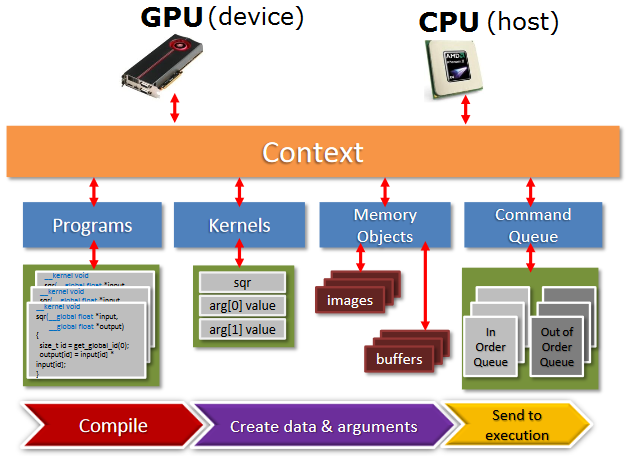
\includegraphics[width=1.0\textwidth]{./images/parallel_programming/opencl_program_flow}
    	\caption{\texttt{OpenCL} program flow and interaction between memory, device and host.}\label{fig:opencl_flow_model}
    \end{figure}

    \begin{description}
    	\item [Contexts creation:]\hfil \\ The first step in every \texttt{OpenCL} application is to create a context and associate to it a number of devices, an available \texttt{OpenCL} platform (there might be present more than one implementation). Each subsequent operation (memory management, kernel compiling and running), is performed within \emph{this} context. In the example \ref{code:openCLContext} a context associated with the CPU device and the first platform returned by OpenCL is created.
    	\lstset{language=[OpenCL]C,
    		caption={\texttt{OpenCL} Context Creation.}, 
    		label={code:openCLContext}, 
    		basicstyle=\ttfamily,
    		keywordstyle=\color{ultramarine}\ttfamily,
    		morekeywords={cl_context,clCreateBuffer,cl_mem_flags,cl_int,size_t},
    		stringstyle=\color{rosemadder}\ttfamily,
    		commentstyle=\color{outerspace}\ttfamily,
    		backgroundcolor=\color{gray!5}, 
    		numbers=left, 
    		numberstyle=\tiny
    	}
    	\begin{lstlisting}
    	cl_int err;
    	cl::vector<cl::Platform> platformList;
    	//Gets a list of available platforms.
    	cl::Platform::get(&platformList); 
   		checkErr(platformList.size()!=0 ?CL_SUCCESS:-1,"cl::Platform::get");
    	cl_context_properties cprops[3] ={CL_CONTEXT_PLATFORM,(cl_context_properties)(platformList[0])(), 0};
    	//create a context based on the first platform from the list
    	//Constructs a context including a list of specified devices
    	cl::Context context(CL_DEVICE_TYPE_CPU,cprops,NULL,NULL,&err);
    	check_error(err, "Conext::Context()"); 
    	\end{lstlisting}

    	\item [Memory buffers creation:]\hfil \\ \texttt{OpenCL} buffer objects on which kernels operates are created at this point using an available and valid context object as shown in Listing \ref{code:opencl_buffer_creation}. 
    	\lstset{language=[OpenCL]C,
    		caption={\texttt{OpenCL} context creation}, 
    		label={code:opencl_buffer_creation}, 
    		keywordstyle=\color{ultramarine}\ttfamily,
    		morekeywords={cl_context,clCreateBuffer,cl_mem_flags,cl_int,size_t},
    		stringstyle=\color{rosemadder}\ttfamily,
    		commentstyle=\color{huntergreen}\ttfamily, 
    		backgroundcolor=\color{gray!5}, 
    		numbers=left, 
    		numberstyle=\tiny
    	}
    	\begin{lstlisting}
    	memobj = clCreateBuffer(context, CL_MEM_READ_WRITE,MEM_SIZE * sizeof(char), NULL, &ret);
    	check_error(err, "Buffer::Buffer()");
    	\end{lstlisting}
    	
    	\item [Build a program:]\hfil \\ 
    	The actual code that runs on the devices has to be compiled first. The \textbf{\textit{cl::Program}} object takes care of building the device code for the devices listed during the context creation. See Listing
    	\ref{code:loadBuildProgramCL} for an example of how \textbf{\textit{cl::Program}} are created.
    	     \lstset{language=[OpenCL]C,
    		caption={\texttt{OpenCL} program load and build}, 
    		label={code:loadBuildProgramCL}, 
    		keywordstyle=\color{ultramarine}\ttfamily,
    		morekeywords={cl_context,clCreateBuffer,cl_mem_flags,cl_int,size_t},
    		stringstyle=\color{rosemadder}\ttfamily,
    		commentstyle=\color{outerspace}\ttfamily,
    		backgroundcolor=\color{gray!5}, 
    		numbers=left, 
    		numberstyle=\tiny
    	}
    	\begin{lstlisting}
    	std::ifstream file("pathToSourceCode.cl");
    	check_error(file.is_open() ? CL_SUCCESS:-1, "pathToSourceCode.cl");std::string
    	prog( std::istreambuf_iterator<char>(file),
    	(std::istreambuf_iterator<char>()));
    	cl::Program::Sources source(1,std::make_pair(prog.c_str(), prog.length()+1));
    	cl::Program program(context, source);
    	err = program.build(devices,"");
    	check_error(err, "Program::build()");
    	cl_kernel kernel = clCreateKernel(program, "nameofthekernel", &ret);
    	\end{lstlisting}
    	
    	
    	\item [Kernel launch:]\hfil \\
    	In order a kernel to be executed a \emph{kernel object} must be created.
    	For a given \emph{Program} there would exists more than one entry point
    	(identified by the keyword \emph{\_\_kernel}. We choose one of them for
    	execution specifying its name in the kernel object constructor.    	
    	 We effectively execute the kernel putting it into a 
    	\emph{cl::CommandQueue}. Given a cl::CommandQueue queue, kernels can be queued
    	using \textit{queue.enqueu\-NDRangeKernel} that queues a kernel on
    	the associated device.
    	Launching a kernel need some parameters (similar to launch configuration in
    	\texttt{CUDA}) to specify the work distribution among
    	work-groups and their dimensionality and size of each dimension (see listing
    	\ref{code:openCLQueuCommand}). We can test the status of the execution by
    	querying the associated \emph{event}.
    	    \lstset{language=[OpenCL]C,
    		caption={\texttt{OpenCL} command queue definition and kernel enqueuing.}, 
    		label={code:openCLQueuCommand}, 
    		keywordstyle=\color{ultramarine}\ttfamily,
    		morekeywords={cl_context,clCreateBuffer,cl_mem_flags,cl_int,size_t},
    		stringstyle=\color{rosemadder}\ttfamily,
    		commentstyle=\color{outerspace}\ttfamily,
    		backgroundcolor=\color{gray!5}, 
    		numbers=left, 
    		numberstyle=\tiny
    	}   
    	\begin{lstlisting}
    	cl::CommandQueue queue(context, devices[0], 0, &err);
	    /*cl_kernel kernel = clCreateKernel(program, "nameofthekernel", &ret);*/
	    kernel.setArg(0,memobj);
	    //let the work-group size be choosen by the implementation 
	    ret = clEnqueueNDRangeKernel(queue, kernel, 1, NULL,
	    &MEM_SIZE, NULL, 0, NULL, NULL)
    	\end{lstlisting}
    \end{description}
\end{description}
 
%%%%%%%%%%%%%%%%%%%%%%%%%%%%%%%%%%%%%%%%%%%%%%%%%%%%%%% 
%\subsection{The Message Passing Interface}

\cleardoublepage

\part{Seamless Acceleration of Numerical Simulation: The \texttt{OpenCAL} framework}
\cleardoublepage
%\chapter[OpenCAL - The Open Computing Abstraction Layer]{The Open Computing Abstraction Layer for Extended
	Cellular Automata and the Finite Differences Method}
\label{ch:opencal}
\dictum[Gottfried Leibniz]{There are two kinds of truths: those of reasoning and those of fact. The truths of reasoning are necessary and their opposite is impossible; the truths of fact are contingent and their opposites are possible.}%
\vskip 1em

\lettrine[lines=3,lhang=0.33,lraise=0,loversize=0.15]{T}{his} chapter introduces \texttt{OpenCAL}, an open source computing
  abstraction layer defining a domain specific language for Extended
  Cellular Automata and the Finite Differences method (see chapters \ref{ch:CA} and \ref{ch:FDM} at page \pageref{ch:CA} and \pageref{ch:FDM} repectively). 
  Different implementations have been developed, which allow for transparent
  parallelism and are able to exploit multicore CPUs and manycore
  devices like GPUs, thanks to the adoption of \texttt{OpenMP} and OpenCL,
  respectively, as well as distributed memory architectures and/or multiple GPUs concurrently.
   System software architecture is presented and the
  underlying adopted data structures and algorithms are described in
  detail. Numerical correctness and efficiency have been assessed by
  considering the well known $SciddicaT$ Computational Fluid Dynamics
  landslide simulation model as reference example.  
  Moreover, a comprehensive study has been performed to device the best platform
  for execution as a function of numerical complexity and
  computational domain extent. Obtained results have highlighted the
  \texttt{OpenCAL} suitability for numerical models development and their execution on
  the most suitable high-performance parallel computational device.
  
\section{Introduction}
\label{sec:opencal_introduction}
 Scientific Computing \cite{golub2014scientific} is a broad and
  constantly growing multidisciplinary research field that uses formal
  paradigms to study complex problems and solve them through
  simulation by using advanced computing techniques and capabilities.
  
   Different formal paradigms have been proposed to provide the
  abstraction context in which problems are formalized. Partial
  Differential Equations (PDEs) were probably the first to be largely
  employed for describing a wide variety of phenomena. Unfortunately,
  PDEs can be analytically solved only for a small set of simplified
  problems \cite{Mazumder20161} and Numerical Methods have to be
  employed to obtain approximate solutions for real life applications. Among
  them, the Finite Differences Method (FDM) was one of the first
  considered, still currently employed, to address a wide variety of
  phenomena such as acoustics \cite{Chaigne19941112, Branski2014},
  heat \cite{Rana2012212, Sahin200619}, computational fluid dynamics
  (CFD) \cite{Chang1990317, Deng201390}, and quantum mechanics
  \cite{Hu2015640, Farrokhabadi201467} and many others.
  
  
  
Besides other solutions proposed for numerically approximating PDEs
  like, for instance, Finite Elements \cite{Hutton:2003} and Finite Volume Methods \cite{Moukalled}, further formal paradigms were more recently proposed for modeling complex systems. Among them, Cellular Automata (CA) \cite{vonNeumann:1966:TSA:1102024} are Turing-equivalent \cite{Codd:1968:CA:1098682, Cook04a} parallel computational models. CA are widely studied from a theoretical point
  of view \cite{Wolfram-1984, Langton-1990b, Wolfram-2002,
    Ninagawa201542}, and their application domains vary from
  Artificial Life \cite{Langton-1986, Beer2004309} to Computational
  Fluid Dynamics \cite{Frish&al-1986, McNamara&Zanetti-1988,
    Higuera&Jimenez-1989, Aidun2010439}, besides many others. See chapter \ref{ch:CA} for an extensive introduction on Cellular Automata.
    
Regardless from the adopted formal paradigm, the simulation of
complex systems often requires the execution of a very large number of computer instruction and this explains why nowadays scientific computing is very oftern linked to  Parallel Computing. 

\texttt{OpenMP} is the  most widely adopted solution for parallel programming on shared
  memory computers \cite{Chapman:2007:UOP:1370966}. It fully supports
  parallel execution on multi-core CPUs and, starting from the 4.0
  release, also includes support of accelerators like graphic
  processing units (GPUs) or Xeon Phi co-processors. Unfortunately,
  compiler support for the $4.0$ release is quite recent and, in
  practice, current \texttt{OpenMP} applications mainly run on CPUs
  \cite{Oliverio2011271, Amritkar2014501, pop:hal-00786675}. However,
  in recent years, general purpose computing on graphic processing
  units (GPGPU), which exploits GPUs and many-core coprocessors for
  general purpose computation, has gained wide acceptance as an
  alternative solution for high-performance computing, resulting in a
  rapid spread of applications in many scientific and engineering
  fields \cite{Owens200780}. Most implementations are currently based
  on NVIDIA CUDA (see e.g. \cite{Blecic2013, DAmbrosio2013630,
    DiGregorio20131183, DAmbrosio201230}), one of the first platforms
  proposed to exploit GPUs computational power on NVIDIA hardware. An
  open alternative to CUDA is OpenCL \cite{Stone201066}, an
  Application Program Inferface (API) originally proposed by Apple and
  currently managed by Khronos Group for parallel programming on
  heterogeneous devices like CPUs, GPUs, Digital Signal Processors
  (DSPs), and Field-Programmable Gate Arrays (FPGAs). Interest in
  OpenCL is continuously growing and many applications can already be
  found in literature \cite{Macri2015328, Bedorf20122825, Du2012391,
    Brown2011898}. However, an OpenCL parallelization of a scientific
  application is often a non-trivial task and, in many cases, requires
  a thorough refactorization of the source code. For this reason, many
  computational layers were proposed, which make many-core
  coprocessors computational power easier to be exploited. For
  instance, ArrayFire \cite{Malcolm2012} is a mathematical library for
  matrix-based computation such as linear algebra, reductions, and
  Fast Fourier transform; clSpMV \cite{Su2012353} is a sparse matrix
  vector multiplication library; clBlas \cite{clBlas-2016} is an
  OpenCL parallelization of the Blas linear algebra library. Examples
  of higher level computational layers, which provide the abstraction
  of formal computational paradigms, are OP2 \cite{Giles20131451},
  which is an open-source framework for the execution of unstructured
  grid applications on clusters of GPUs or multi-core CPUs, AQUAgpusph
  \cite{Cercos-Pita2015295}, which is a smoothed-particle
  hydrodynamics solver, and ASL \cite{asl}, an accelerated
  multiphysics simulation software based, among others, on the Lattice
  Boltzmann Method. Such high-level computational layers are briefly
  overviewed in the next section, together with some other significant
  examples.

This chapter is devoted to the description of \texttt{OpenCAL} which aims to be a portable parallel computing abstraction layer for scientific computing. \texttt{OpenCAL} is released under Lesser GNU Public Licence (LGPL) version 3 and is freely downloadable from GitHub at the following link: \url{https://github.com/OpenCALTeam/opencal}. \texttt{OpenCAL} allows for  the definition of computational models based on CA, XCA and FDM. It is designed to be easily extended and applied to all computational methods based on regular and uniform grids. 
The implementation descripted in this chapter targets shared multicore, distributed memory and GPUs and is designed to make the parallelism transparent to the user addressing and hiding many aspects of the underlying formal computational model and parallel execution platform. 

%\subsection{An Overview on Scientific Simulation Software}
%In this section, we present a non-exhaustive overview of some
%  interesting and widely adopted parallel computing simulation software, which provide a high-level approach for the modeling of complex systems, hiding  low-level implementation issues such as memory allocation/de-allocation, thread management, and I/O  operations.General purpose simulation software,
%  like Mathematica or Matlab, are intentionally not considered here.
%\subsubsection{DEVS}
%  DEVS \cite{Zeigler:1997:DEH:615253.615512, Zeigler:2000:TMS:580780},
%  abbreviation of Discrete Event System Specification, is a modular
%  and hierarchical formalism for modeling and analyzing general
%  systems which can be described in terms of state transition
%  tables. It also allows to describe continuous state systems (which
%  can be formalized in terms of differential equations), and hybrid-
%  continuous state and discrete event systems. The basic DEVS
%  formalism allows to describe the inputs, outputs and states of a
%  model (called atomic), besides the relationships among
%  them. Furthermore, atomics can be used as building blocks for larger
%  coupled models. Both atomic and coupled models adopt the same
%  interface protocol, allowing to use a model as a component in
%  another, larger model. Several extensions to the original DEVS
%  formalism have been developed. Among these, P-DEVS
%  \cite{Chow:1994:PDP:193201.194336} is a modeling formalism which
%  provides both conceptual and parallel execution benefits with
%  respect to the original DEVS formalism, while Cell-DEVS
%  \cite{Wainer:2009:DMS:1611320} is an extension of the DEVS formalism
%  that allows the definition of Cellular Automata models. A wide
%  variety of models have been developed using this approach, such as
%  fire spreading models with different conditions, formation of a
%  watershed and robots in a manufacturing plant
%  \cite{Troccoli:2001:MCP:882496.884491}.
%\subsubsection{OP2}
%  OP2 \cite{Giles20131451} is an open-source framework for the
%  execution of unstructured grid applications on clusters of GPUs or
%  multi-core CPUs. The main characteristic of the library is the use
%  of source-to-source translation to generate efficient back-end code
%  for state-of-the-art hardware for the different target
%  platforms. Specifically, OP2 aims to separate the scientific
%  specification of an application from its parallel implementation to
%  achieve code endurance and near-optimal performance by re-targeting
%  the back-end to different multi-core/many-core hardware. The OP2
%  \emph{active} library approach uses program transformation tools, so
%  that a single application code written using the OP2 API is
%  transformed into the appropriate form that can be linked against a
%  target parallel implementation (e.g. OpenMP, CUDA, OpenCL, MPI,
%  etc.) enabling execution on different back-end hardware
%  platforms. In order to facilitate the development of unstructured
%  mesh applications at a higher hardware agnostic level, OP2 provides
%  both a C/C++ and a Fortran API. This enables application developers
%  to focus on solving problems at a higher level and not worry about
%  architecture specific optimisations. As a consequence, the problem
%  domain space can be separated into both a higher application level
%  to concentrate on solving domain specific problems and write code
%  that remains unchanged for different underlying hardware, and in the
%  meanwhile consider a lower implementation level, that focuses on how
%  a computation can be executed most efficiently on a given platform
%  by carefully analysing the data access patterns.  The performance
%  impact of the library design choices have been quantified on a range
%  of NVIDIA GPUs using the end-to-end performance of an industrial
%  representative CFD application (Airfoil) developed using the OP2
%  API. The full OP2 source, the Airfoil test case code and the
%  auto-tuning framework are available as open source software
%  \cite{OP2Web}.
%\subsubsection{CAMELot}
%  CAMELot \cite{dattilo2003simulation, Mendicino2006, d2007parallel}
%  is a proprietary CA and XCA high performance simulation environment
%  derived from CAMEL \cite{cannataro1995parallel}. The system supports
%  CARPET, a purpose-built language for CA programming based on C with
%  additional constructs to describe the rule of the state transition
%  function of a single cell of a cellular automaton and, eventually, to steer the
%  application. Specifically, a CARPET program is composed of a declaration part that
%  describes the properties of CA (dimension, radius, state, neighbour,
%  parameters, region), a body program that implements the transition
%  function, and a steering part that contains a set of commands for
%  extracting and analysing system information and performing
%  computational steering (i.e., global operations). The steering
%  section is performed by the runtime system at each iteration, after
%  the transition functions of all cells have been evaluated.  The
%  state of a cell is defined as a record of typed \emph{substates}
%  (char, shorts, integers, floats, doubles and one-dimensional
%  arrays), and even complex neighbourhoods (e.g., hexagonal, Margolus)
%  can be simply defined by means of a CARPET
%  statement. Non-deterministic, time-dependent and non-uniform
%  transition functions can also be defined. Camelot offers an
%  integrated programming environment, an interactive user interface
%  and permits the efficient and seamless simulation of XCA on
%  distributed memory computers.
%\subsubsection{libAuToti}
%  An open-source alternative to CAMELot is libAuToti
%  \cite{spingola2008modeling}, an efficient and flexible parallel XCA
%  library. Similarly to CAMELot, libAuToti allows for a simple and
%  concise definition of both the transition function and the other
%  characteristics of XCA model definition. It allows for both
%  sequential and parallel execution, both on shared and distributed
%  memory machines (thanks to the adoption of the Message Passing
%  paradigm for the interprocesses communications), by hiding parallel
%  implementation issues to the user. The library also implements a
%  dynamic load balancing algorithm to better exploit computational
%  resources and reduce overall execution time
%  \cite{DBLP:conf/csc/ZitoDSSRA09}. A multithread version was also
%  developed to better exploit multi-core architectures, coupled with
%  an interactive 2D/3D visualization system based on VTK
%  \cite{spataro2010multithread}.
%\subsubsection{ASL}
%  The Advanced Simulation Library (ASL) \cite{asl} is a free and open
%  source hardware accelerated multiphysics simulation software. It is
%  based, among others, on the Lattice Boltzmann Method and is written
%  in OpenCL, which enable efficient deployment on a variety of
%  massively parallel architectures. However, no OpenCL knowledge is
%  strictly required to develop ASL-based applications, thanks to a
%  simplified C++ API. ASL can be used to model various coupled
%  physical and chemical phenomena and employed in a multitude of
%  fields like computational fluid dynamics, computer-aided
%  engineering, and crystallography.  Mesh-free, immersed boundary
%  approach allows to move from CAD directly to computations
%  eliminating pre-processing efforts and reducing amount of potential
%  errors.
%\subsubsection{AQUAgpusph}
%  Eventually, AQUAgpusph \cite{CercosPita2015295} is a free Smoothed
%  Particle Hydrodynamics (SPH - a mesh-free Lagrangian method to solve
%  Navier-Stokes equations) software accelerated with OpenCL. The main
%  advantages with respect to other existing SPH libraries are the use
%  of OpenCL instead of CUDA, which allows for parallel execution on a
%  variety of massively parallel devices, the implementation of the
%  most popular boundary conditions, the easy customization of the code
%  to different problems, the extensibility with regard to Python
%  scripts and the runtime output which allows the tracking of
%  simulations in real time, or a higher frequency in saving some
%  results without a significant performance lost. Authors have proven
%  to improve the solver speed, the results quality, and the usability
%  for a wider areas of application.
  
\section[Software Architecture]{\texttt{OpenCAL} Software Architecture and the Considered Parallel Computing Paradigms}
  This section describes the software architecture of the first
  \texttt{OpenCAL} release. As described in Figure \ref{fig:architecture}, a
  computational model can be designed at the higher level of
  abstraction. As already stated, supported computational paradigms
  are CA, XCA and FDM. At this level, the main features of the
  computational model like dimensions, neighborhood, boundary
  conditions, involved substates and elementary processes, are
  designed. The simulation process, which allows to obtain the model
  evolution at discrete time steps, is also defined at this level, by
  specifying the initial condition of the system, global operations
  (like steering or global reductions), the initial and final
  computational step and a possible stopping criterion. Eventually,
  optimizations can be considered, namely the explicit update, which
  allows to selectively update substates after the application of each
  elementary process, and the quantization feature, which allows to
  restrict the computation to a subset of the computational domain, by
  excluding stationary cells.
  
  \begin{figure}
  	\begin{center}
    \includegraphics[width=1.0\textwidth]{./images/opencal/Figure05}
    \caption{\texttt{OpenCAL} architecture. At the higher level of abstraction, the models,
    	as well as the simulation process, and possible optimizations are
    	designed. \texttt{OpenCAL} can be found at the implementation abstraction
    	layer, allowing for a straightforward implementation of the designed
    	model. In fact, it can be considered as a domain-specific language for
    	the CA, XCA and FDM computational methods, built on top of the C
    	language and the \texttt{OpenMP} and OpenCL APIs. \texttt{OpenCAL} applications can be
    	executed at the hardware level on both multi-core CPUs and many-core
    	devices, while the execution on cluster is planned but currently not
    	supported.}
    \label{fig:architecture}
  \end{center}
\end{figure}
  
   \texttt{OpenCAL} can be found in the implementation abstraction level. As it
  can be seen, four different versions can be considered for
  implementing the previously designed computational model, namely
  \texttt{OpenCAL}, \texttt{OpenCAL-OMP} and \texttt{OpenCAL-CL} and \texttt{OpenCAL-MPI}. The first one refers to the   serial implementation of the library, while second and the third are \texttt{OpenMP}  and OpenCL-based parallelizations, respectively, as pointed out by
  the language/low-level library level. The fourth one is a cluster ready implementation that allows to execution on distributed memory cluster where each node can exploit multiple GPUs.
  All implementations are written in C for the maximum efficiency and provide high-level data types and functions that match the XCA formal components, allowing  for a straightforward implementation of the designed computational
  model, by also allowing to ignore low-level issues like memory
  management and I/O operations. In this respect, \texttt{OpenCAL} can be
  considered as a domain-specific language (DSL) for the CA, XCA and
  FDM computational methods. Finally, at the hardware level, depending
  on the adopted version of the library, execution can be performed on
  single- and multi-core CPUs, or on many-core accelerators like GPUs,
  almost transparently to the user.
  
   Figure \ref{fig:architecture} also shows hybrid MPI+Open-MP and
  MPI+OpenCL parallel implementations of \texttt{OpenCAL}, which will allows to
  exploit clusters of CPUs and many-core accelerators. 

  Note that an \texttt{OpenMP}-based parallelization is generally more
  straightforward with respect to one based on OpenCL or MPI and, when
  compilers will fully support the 4.0/4.5 \texttt{OpenMP} specifications, it
  will be possible to execute \texttt{OpenMP}-based applications on both
  multi-core CPUs and many-core high-performance devices. On the other
  hand, an OpenCL-based parallelization allows to exploit a wide range
  of high-performance many-core devices straight away and, with greater control on the underlying hardware and on the execution flow, allowing better exploitation of the hardware capabilities. 
 For these reasons, both the \texttt{OpenMP} and OpenCL versions of \texttt{OpenCAL} have been developed and are maintained. 
  
\section{The Open Computing Abstraction Layer}
\label{sec:OpenCAL}
In this section we describe the API of the serial version of
\texttt{OpenCAL}, which allows for the definition of 2D and 3D CA, XCA and
FDM models, and their execution on CPUs. Nevertheless, 1D models can
also be defined as degenerate case of 2D ones. The implementation of
a simple 2D CA, namely the \textit{Conway's Game of Life}
\cite{gardner1970a}, is shown in this section as first and
straightforward example of application.

\subsection{API naming Convention}
In \texttt{OpenCAL}, besides the three basic supported scalar data types,
namely \verb'CALbyte', \verb'CALint', and \verb'CALreal', which
redefine the \verb'char', \verb'int' and \verb'double' C native
scalar data types, respectively, the API adopts the following
conventions:
\begin{itemize}
	\item Derived data types are characterised by the \verb'CAL' prefix,
	followed by a type identifier formed by one or more capitalised
	keywords, an optional suffix identifying the model dimension
	(\verb'2D' or \verb'3D'), and an eventual optional suffix
	specifying the basic scalar type (\verb'b', \verb'i', or \verb'r',
	for \verb'CALbyte', \verb'CALint' and \verb'CALreal' derived
	types, respectivey);
	\item Constants and enumerals are characterised by the \verb'CAL_'
	prefix, followed by one or more uppercase keywords separated by
	the \verb'_' character (e.g. the \verb'CAL_TRUE' and
	\verb'CAL_FALSE' boolean-type values);
	\item Functions are characterised by the \verb'cal' prefix, followed
	by at least one capitalized keyword, and end with a suffix
	specifying the model dimension (\verb'2D' or \verb'3D') and the
	basic datatype (\verb'b', \verb'i', or \verb'r', for
	\verb'CALbyte', \verb'CALint' and \verb'CALreal' derived types,
	respectively).
\end{itemize}
Moreover, the \verb'{arg1|arg2|...|argn}' and
\verb'[arg1|arg2|...|argn]' conventions are adopted in the
following. The first one identifies a list of $n$ mutually exclusive
arguments, where one of the arguments is needed, while the second a
list of $n$ non-mutually exclusive optional arguments.

Among derived data types, \verb'CALParameter{b|i|r}' represents an
alias for the corresponding basic \texttt{OpenCAL} scalar data type, and can
be optionally used for defining model parameters.


\subsection{API}
An \texttt{OpenCAL} model is declared as a pointer to \verb'CALModel{2D|3D}'
and defined by means of the \verb'calCADef{2D|3D}()' function. The
model object stores the dimensions of the computational domain in
terms of number of rows and columns (and also slices in case of a 3D
model), the computational domain boundary topology (e.g., if a 2D
computational domain has to be considered as a bounded or an
unbounded torus), the neighbourhood pattern, and also registers
pointers to substates and elementary processes composing the
transition function. Moreover, it manages a sub-structure which
allows to exploit the built-in quantization feature by means of
which, based on user-specified criteria, the computation can be
restricted to a subset of non-stationary cells (also called active
cells) of the whole computational domain.

 As regards neighborhoods, \texttt{OpenCAL} provides a set of predefined
patterns. For instance, the \verb'CAL_MOORE_NEIGHBORHOOD_{2D|3D}'
enumeral refers to the Moore pattern (cf. Figures
\ref{fig:2Dneighborhood}b and \ref{fig:3Dneighborhood}b). von
Neumann 2D and 3D neighborhoods are also predefined, as well as 2D
hexagonal patterns (cf. Figures \ref{fig:2Dneighborhood}c and
\ref{fig:2Dneighborhood}d). Custom neighborhoods can also be defined
in \texttt{OpenCAL} by considering the \verb'CAL_CUSTOM_NEIGHBORHOOD_{2D|3D}'
enumeral and the \verb'calAddNeighbor{2D|3D}()' function, which adds
a cell to the neighbourhood by means of its relative coordinates
with respect to the central one. Note that, a zero-based index is
assigned to the neigbouring cells in order to address them without
the need to provide their relative coordinates, as shown in Figures
\ref{fig:2Dneighborhood} and \ref{fig:3Dneighborhood}.
\begin{figure}[!htbp]
	\begin{center}
		\includegraphics[width=1.0\textwidth]{./images/opencal/Figure01}
		\caption{Examples of von Neumann (a) and Moore (b) neighborhoods for two-
			dimensional CA with square cells. Examples of Moore neighborhoods are also shown for hexagonal CA, both for the cases of horizontal (c) and vertical (d) orientations. Central cell is represented in dark gray, while adjacent cells are in light gray. A reference system is here considered to evaluate cells coordinates in terms of row and column indices in a matrix-style representation, and a 0-based numerical identifier assigned to each cell in the neighborhood for straightforward access}
		\label{fig:2Dneighborhood}
	\end{center}
\end{figure}
Elementary processes, both local interactions and internal
transformations, are defined by means of callback functions and
registered to a computational model by means of the
\verb'calAddElementaryProcess{2D|3D}()' function. Each elementary
process callback must return \verb'void' and takes a list of integer
arguments, representing the coordinates of a generic cell in the
computational domain. Elementary processes define the \texttt{OpenCAL}
transition function, and can be implicitly applied by the simulation
loop to the cells of the computational domain in the same order in
which they were registered to the computational model, or in a user
defined order (cf. below).


\begin{figure}[!htbp]
	\begin{center}
		\includegraphics[width=1.0\textwidth]{./images/opencal/Figure04}
		\caption{Examples of von Neumann (a) and Moore (b, b') neighborhoods for
			three-dimensional CA with cubic cells. Central cell is represented in
			dark gray, while adjacent cells are in light gray. A reference system
			is here considered to evaluate cells coordinates in terms of row,
			column and slice indices in a matrix-style representation, and a
			0-based numerical identifier assigned to each cell in the neighborhood
			for straightforward access.}
		\label{fig:3Dneighborhood}
	\end{center}
\end{figure}
Substates are defined as pointers to
\verb'CALSubstate{2D|3D}{b|i|r}' and can be registered by means of
the \verb'calAddSubstate{2D|3D}{b|i|r}()' function. Substates are
internally defined by means of two linearized arrays (also called
computational layers), having the same dimensions of the
computational domain. The \emph{current} layer is used as a
read-only memory for retrieving central and neighboring cells
current states, while the \emph{next} one for updating the new value
for the central cell. This is a commonly adopted solution for
obtaining the \emph{implicit parallelism}, thanks to which cells
appear to be simultaneously updated with respect to each other, even
in the case of serial computation. Single layer substates can be
also defined in \texttt{OpenCAL} by simply registering them through the
\verb'calAddSingleLayerSubstate{2D|3D}{b|i|r}()' function. In this
case, they only consist of the current computational layer, and can
be used for internal transformations processing. To retrieve the
current value of a substate for a (central) cell by providing its
coordinates within the computational domain, the
\verb'calGet{2D|3D}()' function can be adopted, while the
\verb'calGetX{2D|3D}()' function can be considered for obtaining the
same information for a neighbouring cell, by providing an additional
parameter specifying the index of the cell in the neighborhood
(cf. Figures \ref{fig:2Dneighborhood} and \ref{fig:3Dneighborhood}
for predefined neighborhoods). Eventually, the
\verb'calSet{2D|3D}()' function can be used to set the new value of
a substate for the (central) cell to the next computational
layer. In the case of a single layer substate, the
\verb'calSetCurrent{2D|3D}{b|i|r}()' function has to be employed for
updating purposes. It acts like the \verb'calSet{2D|3D}()' function,
with the exception that the new value is written on the current
computational layer. Note that, after the application of each
elementary process, all the registered substates are implicitly
updated, i.e. the next layer is copied into the current
one. However, this behaviour can be overridden and substates
explicitly, as well as selectively, updated by means of the
\verb'calUpdateSubstate{2D|3D}{b|i|r}' function
(cf. below). Obviously, single layer substates do not need to be
updated.

The \texttt{OpenCAL} quantization feature is implemented by considering a
dynamic array of active cells, $A$, which is initially empty. An
array of flags, $F$, having the same dimension of the computational
domain is also considered, which is initially set to
\verb'CAL_FALSE' in each position. Eventually, an integer variable,
$size$, initially set to zero, is used to evaluate the new dimension
of $A$ per effect of the add/remove operations. In order to add a
cell to $A$, the \verb'calAddActiveCell{2D|3D}()' function can be
used, which sets the flag value to \verb'CAL_TRUE' in the
corresponding position of the array $F$ and increases $size$ by
one. Similarly, the \verb'calAddActiveCellX{2D|3D}()' function adds
a neighbouring cell to $A$. Eventually, the
\verb'calRemoveActiveCell{2D|3D}()' function can be used to remove a
cell from $A$, by contextually modifying the corresponding flag in
$F$ and decrementing $size$ by one. When an add/remove stage is
completed, e.g. after the execution of an elementary process, and
the (scattered) array $F$ is well defined, the set $A$ must be
updated. The update process deletes the current set $A$, allocates a
new set of active cells of dimension $size$, and applies a
straightforward serial stream compaction algorithm by processing the
entire array of flags $F$, as shown in Figure
\ref{fig:active_cells}. As evident, the algorithm has a $O(n)$
computational efficiency, being $n$ the number of cells of the
cellular space $R$. In this way, only the loop updating $A$ occurs
on the whole computational domain (since the $F$ array must be fully
checked). In fact, when $A$ is not empty, it is processed instead of
the whole computational domain and both elementary processes
computation and substates updating take place on the active
cells. As substates, even $A$ is implicitly updated at the end of
each elementary process. However, active cells update can also be
explicitly performed by means of the
\verb'calUpdateActiveCells{2D|3D}' function (cf. below).
Eventually, note that the add and remove stages updating the values
in $F$ have to be performed separately, e.g. by two different
elementary processes. In fact, if the same elementary process could
both add and remove cells depending for instance on the current
state of the central cell, two different cells could update the same
(neighbouring) cell to different activation states, and the
resulting value in $F$ would depend on the (serial) application
order of the elementary process, giving rise to a possible logical
error.

\begin{figure}
	\begin{center}
		\includegraphics[width=1.0\textwidth]{./images/opencal/Figure06}
		\caption{An example of application of the serial stream compaction algorithm
			adopted to update the set $A$ of active cells in the serial
			implementation of \texttt{OpenCAL}. In the example, active cells are
			represented in gray within a two-dimensional 4x4 matrix of flags,
			implemented as a linearized array, $F$. The stream compaction
			algorithm simply processes $F$ and produces the compacted array $A$ as
			output, containing the coordinates of the active cells. The global
			state transition is therefore limited to the cell in $A$, and a new
			configuration of the system obtained. The process is therefore
			repeated at the next computational step.}
		\label{fig:active_cells}
	\end{center}
\end{figure}

In order to perform a simulation, a pointer to \verb'CALRun{2D|3D}'
must be declared and defined by means of the
\verb'calRunDef{2D|3D}()' function. The simulation object stores a
pointer to the \texttt{OpenCAL} model to be run, a step counter, the initial
and final computational steps, an enumeral of type
\verb'CALUpdateMode', which specifies the substates update policy
(if implicit or explicit), and registers a set of four optional
callback functions. These latter, described below, take a pointer to
an \texttt{OpenCAL} model as argument and do not return any value, with the
exception of the termination function, which returns a
\verb'CALbyte' (\verb'CAL_TRUE' if the termination criterion is
satisfied, \verb'CAL_FALSE' in the other case). The optional
callback functions are:
\begin{itemize}
	\item \verb'init()': It can be used to set the initial conditions of
	an \texttt{OpenCAL} computational model. It can be registered to the
	simulation object by using the \verb'calRunAddInitFunc{2D|3D}()'
	function. If defined, the \verb'init()' function is executed once
	before the simulation loop.
	\item \verb'globalTransition()': It can be used to redefine the
	execution order of the registered elementary processes and to
	perform selective substate updating. The
	\verb'calApplyElementaryProcess{2D|3D}()' function can be used
	within the registered callback to apply a registered elementary
	process to each cell of the computational domain, while the
	\verb'calUpdateSubstate{2D|3D}{b|i|r}' to update a registered
	substate. The \verb'globalTransition()' function also allows to
	call functions that can perform global operations over the
	computational domain, e.g. reductions. It can be registered to the
	simulation object by using the
	\verb'calRunAddGlobalTransitionFunc{2D|3D}()' function. If
	defined, the \verb'globalTransition()' function overrides, i.e. is
	applied instead of, the implicit global transition function.
	\item \verb'steering()': It can be used to perform global
	operations, e.g. reductions, at the end of each computational
	step, that is after that all the elementary processes have been
	applied. Predefined reductions allow to compute global minimum,
	maximum, sum, product, as well as logical and bit-wise AND, OR and
	NOT operations on the registered substates. A steering can be
	registered to the simulation object by using the
	\verb'calRunAddSteeringFunc{2D|3D}()' function. If defined, the
	\verb'steering()' function is applied at the end of each
	computational step.
	\item \verb'stopCondition()': It can be used to define a stopping
	criterion for the simulation. Note that, if the last computational
	step was set to \verb'CAL_RUN_LOOP', the \verb'stopCondition()'
	callback is mandatory to stop the simulation. It returns
	\verb'CAL_TRUE' if the termination criterion is satisfied,
	\verb'CAL_FALSE' in the other case. The termination callback can
	be registered by using the
	\verb'calRunAddStopConditionFunc{2D|3D}()' function. If defined,
	the \verb'stopCondition()' function is executed at the end of each
	computational step.
\end{itemize}
The simulation process can be executed by means of the
\verb'calRun{2D|3D}' function. Algorithm \ref{algo:simuloop}
outlines the \texttt{OpenCAL} implicit simulation process, which takes place
in the case the enumeral \verb'CAL_UPDATE_IMPLICIT' was used as last
argument for the \verb'calRunDef{2D|3D}()' function. The
\verb'init()' function, if defined, is called first and then active
cells (if quantization is enabled) and substates are
updated. Moreover, the \verb'step' counter and the \verb'halt'
variable, that is used to check the simulation termination
condition, are set to the initial step and to \verb'CAL_FALSE',
respectively. The main simulation loop follows, which applies
elementary processes in the order they were registered to each cell
of the computational domain. After the execution of each elementary
process, active cells and substates are updated. If defined, the
\verb'steering()' global function is therefore called and active
cells and substates updated. The \verb'stopCondition()' function is
also called and the step counter increased. The simulation loop
continues while the \verb'halt' variable, whose value is set by the
\verb'stopCondition()' function, is \verb'CAL_FALSE' or the final
step of computation is met.

\begin{algorithm}
	\DontPrintSemicolon \SetKwFunction{Init}{init()}
	\SetKwFunction{Update}{update}
	\SetKwFunction{Steering}{steering()}
	\SetKwFunction{Stop}{stopCondition()}
	\SetKwFunction{Finalize}{finalize()}
	
	\Init \tcp*{Call the \Init global function}
	 \If{quantization}{
		\Update($A$) \tcp*{Update the array of active cells}
	 }
	\ForAll{$q \in Q$}
		{ \Update($q$) \tcp*{Update the substate $q$}
		}
	$step \gets initial\_step$\; $halt \gets false$\;
	\While{$\neg$halt $\land$ (step $\leq$ final\_step $\vee$
		final\_step = CAL\_RUN\_LOOP)}{
		 \ForAll{$e$ of $\sigma$}{
			\ForAll{$(A \neq \emptyset \land i \in A) \vee$ $i \in R$}
				{
				$e(i)$ \tcp*{Apply the elementary process $e$ to the cell
					$i$}
				}
			\If{quantization}{
				 \Update($A$) \tcp*{Update the array of active cells} 
			}
			\ForAll{$q \in Q$}{ 
				\Update($q$) \tcp*{Update the substate $q$}
			 }
		  }
	  	\Steering \tcp*{Call the \Steering global function}
	  	 \If{quantization}{
	  	 	 \Update($A$) \tcp*{Update the array of active cells}
  	 	  } 
   	  	\ForAll{$q \in Q$}{
			\Update($q$) \tcp*{Update the substate $q$}
		 }
		 $halt \gets $\Stop \tcp*{Check the stop condition} $step \gets step + 1$\;
	 }
	\Return\;
	\caption{{\texttt{OpenCAL} main implicit simulation process.}}
	\label{algo:simuloop}
\end{algorithm}

Explicit update can be set by using the \verb'CAL_UPDATE_EXPLICIT' enumeral as last argument of the \verb'calRunDef{2D|3D}()' function. In this case, the global transition function must be overridden and both active cells and substates explicitly updated. Eventually, instead of the \verb'calRun{2D|3D}()', which executes the whole simulation process, the
\verb'calRunCAStep{2D|3D}()' function can be used to apply a single
step of the global transition function, including steering and stop
condition checking. In this case, the initialization function must
be called explicitly, as well as the simulation counter increased.




\subsection{\texttt{OpenCAL} Conway's Game of Life}
As a first illustrative example, we here present the \texttt{OpenCAL}
implementation of the Turing complete Conway's Game of Life\cite{gardner1970a}, one of the most simple, yet powerful examples of CA, devised by mathematician John Horton Conway in 1970. See Section \ref{sect:GOL} at page \pageref{sect:GOL} for a formal definition of \textit{The Game of Life} and a  description of its governing rules.

The program in Listing \ref{lst:cal_life} provides a complete
\texttt{OpenCAL} implementation of Game of Life in just few lines of code,
by defining both the CA model and the simulation object, needed to
let the CA evolve step by step.

%%%% GOL listing C serial implementation %%%%
    \lstset{language=[OpenCL]C,
	caption=An \texttt{OpenCAL} implementation of the Conway's Game of
	Life., 
	label=lst:cal_life, 
	basicstyle=\footnotesize\ttfamily,
	keywordstyle=\color{blue}\ttfamily,
	stringstyle=\color{red}\ttfamily,
	commentstyle=\color{green}\ttfamily,
	backgroundcolor=\color{light-gray}, 
	numbers=left, 
	numberstyle=\tiny
}
\lstinputlisting{./code/cal_life.c}
%%%%%%%%%%%%%%%%%%%%%%%%%%%%%%%%%%%%%%%%%%%%
\texttt{OpenCAL} header files are included at lines 1-3. Specifically,
\verb'cal2D.h' allows to define 2D CA and substates,
\verb'cal2DRun.h' the simulation object, while \verb'cal2DIO.h'
provides some basic I/O functions. The CA object is declared at
line 6, while lines 7 and 8 declare a substate and a simulation
object, respectively.  Objects declared at lines 6-8 are defined
later in the \verb'main' function. In particular, the \verb'life'
CA object is defined at line 24 by the \verb'calCADef2D()'
function. The first 2 parameters define the dimensions of the
computational domain (in terms of number of rows and columns,
respectively), while the third the Moore
neighborhood. Furthermore, the fourth parameter sets a toroidal
topology for the cellular space, while the last switches the
active cells optimization to off.

The CA simulation object is defined at line 25 by the
\verb'calRunDef2D()' function, where the first parameter is a
pointer to the \verb'life' CA object, while the second and third
parameters specify the initial and last simulation steps,
respectively. Eventually, the last parameter sets the update
policy to implicit.

Line 27 allocates memory and registers the integer-based $Q$
substate to the CA by means of the \verb'calAddSubstate2Di()'
function, while line 29 registers an elementary process by means
of the \verb'calAddElementaryProcess2D()' function. Here, the
\verb'lifeTransitionFunction' parameter represents the name of a
developer-defined function implementing the transition function
rules (cf. lines 10-20). Within the elementary process, the
\verb'calGet[X]2Di()' and \verb'calSet2Di()' functions are used
for reading and updating purposes, respectively. The
\verb'calInitSubstate2Di()' function at line 31 sets the whole $Q$
substate to the value 0 (for both the current and next
layers). Lines 32-36 define a so called \emph{glider} pattern
(cf. Figure \ref{fig:cal_life_glut}a) by means of the
\verb'calInit2Di()' function. The \verb'calSaveSubstate2Di()'
function at line 38 saves the $Q$ substate to file, while the
\verb'calRun2D()' function at line 40 enters the simulation
process (actually, only one computational step in this example),
and returns to the \verb'main' function when the simulation is
terminated. The \verb'calSaveSubstate2Di()' is called again at
line 42 to save the new (last) configuration of the CA, while the
last two functions at lines 44 and 45 release memory previously
automatically allocated by \texttt{OpenCAL} for the CA, substates
(actually, only $Q$ in this case) and simulation object. The
\verb'return' statement at line 47 ends the program.

Figure \ref{fig:cal_life_glut} show a graphical representation of
the initial and final configurations of Game of Life,
respectively, as implemented in Listing \ref{lst:cal_life}. As
expected, the glider initially defined has evolved into the new
correct configuration.

\begin{figure}
	\begin{center}
		\includegraphics[width=1.0\textwidth]{./images/opencal/Figure07.pdf}
		\caption{An \texttt{OpenGL/GLUT} version of the Game of Life, as implemented in Listing \ref{lst:cal_life}, showing the (a) initial and (b) final configurations of the system. Alive cells are represented in white, dead cells in blue.}
		\label{fig:cal_life_glut}
	\end{center}
\end{figure}

\section{The \texttt{OpenCAL} \texttt{OpenMP}-based Parallel Implementation}
\label{sec:OpenCAL-OMP}

In this section we present \texttt{OpenCAL-OMP}, the \texttt{OpenMP}-based parallel
implementation of \texttt{OpenCAL}, which allows for seamless parallel execution on
shared memory computing systems in a SIMD fashion. For brevity, we
only present and discuss differences with respect to \texttt{OpenCAL} in
terms of API and internal algorithms.
Since one of the main goal is to obtain transparent parallelism, the \texttt{OpenCAL-OMP} API has been designed to differ as less as possible to the serial
one, leading to the adoption of the same naming conventions, interface,
and programming model.

Double layer substates were also considered in \texttt{OpenCAL-OMP}, which permitted a straightforward lock-free \texttt{OpenMP} parallelization. In fact no race conditions can occur, since the current layer is accessed in read mode, and the update phase access to the next layer is limited to the memory location associated with
the central cell. As a consequence, elementary processes and
substates updating loops, as well as global reduction operations,
were parallelized by simply considering lock-free \texttt{OpenMP} pool of
threads, as shown in Figure \ref{fig:pool_of_threads}. In the
example, a pool of three threads were used to partition the
computational domain in three subregions, which were therefore
processed in parallel both during the application of an elementary
process and the subsequent substates updating. Note that, in the
case only a subset of cells are actually involved in computation, as
in the example, load unbalance conditions can occur. In fact, the
third thread is wasted, since it only applies the elementary process
on a subset of stationary cells. A dynamic \texttt{OpenMP} scheduling is
adopted in this case to mitigate the unbalance among chunks.
\begin{figure}
	\begin{center}
		\includegraphics[width=1.0\textwidth]{./images/opencal/Figure08.pdf}
		\caption{An example of \texttt{OpenCAL-OMP} parallel application of an elementary
			process to a substate $Q$ and its subsequent parallel updating. The
			computational domain is initially partitioned by means of a pool of
			three threads (fork phase). These latter concurrently apply the
			elementary process by reading state values from the current layer and by updating new values to the next one. At the end of the elementary process application, threads implicitly synchronize by joining into the master one (join phase), and the parallel update phase starts. As before, a pool of threads concurrently copies the next layer into the current one and the new configuration of $Q$ is obtained. A join phase eventually occurs, which ensures data consistency before the application of another elementary process.}
		\label{fig:pool_of_threads}
	\end{center}
\end{figure}
As regards the quantization feature, it is still based on the
dynamic array of active cells $A$, containing the coordinates of non
stationary cells, and on the array of flags $F$, having the same
dimension of the computational domain, used to register the cells
activation state during the application of the transition
function. $F$ is initially set to \verb'CAL_FALSE' in each position
and, each time a cell has to be added to/removed from $A$, the
corresponding position in $F$ is updated by a \verb'CAL_TRUE'/\verb'CAL_FALSE' value. 
At the end of the add/remove
stage, a lock-free parallel stream compaction is executed on the
resulting scattered array $F$ to obtain the new set of active cells
$A$. For this purpose, $F$ is partitioned over the $N$ running
threads. Each of them builds a private subset, $A_p$ $(p=0, 1,
\ldots N-1)$, of cells to be added to/removed from $A$, by
contextually evaluating its relative size, $size_p$. Eventually, the
actual $size$ of $A$ is obtained as $size = \sum_{p=0}^{N-1}
size_p$, and the subsets $A_p$ assembled together to form the new
set $A$, as shown in Figure \ref{fig:active_cells_omp}. As for the
case of the \texttt{OpenCAL} serial stream compaction, it is evident that
also in this case the algorithm has a $O(n)$ computational
efficiency, where $n$ is the number of cells of the cellular
space. Note that, being both the \verb'CAL_TRUE' and \verb'CAL_FASE'
8-bit long enumerals, no inconsistent values can be obtained even in
the case more than one thread accesses the same location in $F$
simultaneously and, therefore, a lock-free updating policy was also
here considered for the quantization optimization. However, as for
\texttt{OpenCAL}, the add and remove stages updating the values in $F$ have
to be performed separately, e.g. by two different elementary
processes, in order to avoid possible race conditions. In fact, if
the same elementary process could both add and remove cells
(depending for instance on the current state of the central cell),
two different threads applying the elementary process to two
different cells could update the same (neighbouring) cell to
different activation states. In this case, the resulting value in
$F$ would depend on which thread writes the value for last, giving
rise to a possible logical error. Eventually, note that the
quantization feature is able to optimally distribute the
computational load over the running threads, since stationary cells
are simply excluded by the computation (cf. Figure
\ref{fig:active_cells_omp}). A more efficient static \texttt{OpenMP}
scheduling is therefore here adopted instead of the dynamic one.

\begin{figure}
	\begin{center}
		\includegraphics[width=1.0\textwidth]{./images/opencal/Figure09}
		\caption{An example of application of the parallel stream compaction algorithm used in \texttt{OpenCAL-OMP} to update the set $A$ of active cells. Active cells are represented in gray within a two-dimensional 4x4 matrix of flags, implemented as a linearized array, $F$. The parallel stream
			compaction algorithm processes $F$ by means of a lock-free pool of
			threads, resulting in the $A_p$ $(p=0,1,2)$ partial arrays of active
			cells. These latter are eventually assembled together by the master
			thread, resulting in the compacted array $A$. A new pool of threads
			therefore applies the state transition function in parallel on $A$
			with an optimal load balancing, and a new configuration of the system
			is obtained. The process is therefore repeated at the next
			computational step.}
		\label{fig:active_cells_omp}
	\end{center}
\end{figure}


\subsection{\texttt{OpenCAL-OMP} implementation of the Game of Life}
Conway's Game of Life can be straightforwardly implemented in
parallel by using \texttt{OpenCAL-OMP}. The source code is almost identical
to the one in Listing \ref{lst:cal_life}, with the exception of
the first three lines, where the \texttt{OpenCAL-OMP} header files are
included instead of the OpenCAL ones. For this purpose, it is
sufficient to change the headers parent directory from
\verb'OpenCAL' to \verb'OpenCAL-OMP'. For instance, the
\verb'OpenCAL/cal2D.h' header is replaced by
\verb'OpenCAL-OMP/cal2D.h'. The remaining lines of code are
unchanged and therefore source code is omitted. As for the case of
the \texttt{OpenCAL} implementation, Figure \ref{fig:cal_life_glut} shows
the initial and final configuration of the system.


\section{The \texttt{OpenCAL} OpenCL-based Parallel Implementation}
\label{sec:OpenCAL-CL}
  In this section, we present the OpenCL-based parallel implementation
of OpenCAL, which allows for the parallel execution on both shared
memory computing systems and many-core acceleration devices in a
SIMD fashion, by highlighting the differences with respect to the
serial and OpenMP implementations of OpenCAL in terms of API and
internal algorithms.

The API is very similar to the serial one and adopts the same
programming model and naming conventions, with the exception that
the \verb'calcl', \verb'CALCL' and \verb'CALCL_' prefixes are
adopted for functions, data types and constants, respectively. The
main difference with respect to OpenCAL and OpenCAL-OMP is that an
OpenCAL-CL application is subdivided in two parts, one running on
the CPU, the other in parallel on a compliant device. The host
application defines the host-side computational model, registers the
required substates to it, while elementary processes and other
global function are implemented as OpenCL kernels and registered to
a device-side computational model. When a device-side model is
defined, data registered to the host-side model is implicitly copied
to the compliant device global memory, transparently to the
user. Within kernels, however, the user can transfer data to the
local memory and then update the global memory when the local
operations are complete, for better performance. Data stored in
global memory is therefore copied back to the host at the end of
the simulation process. This latter if equivalent to that of OpenCAL
and OpenCAL-OMP (cf. Algorithm \ref{algo:simuloop}), with the
exception that kernels are executed device-side and the simulation
process can not be currently, in this first OpenCAL release, made explicit.

Grid of work-items can be two- or three-dimensional, depending on
the dimension of computational model, if 2D or 3D, respectively. In
the case the quantization feature is exploited, a one-dimensional
grid is considered. The number of work-items is evaluated for each
model dimension by preliminary querying OpenCL for the
(device-dependent) preferred work-group size multiple (i.e. the
warp/wavefront size in NVIDIA/AMD GPUs), $w_s$, and therefore by
considering the smallest multiple of $w_s$ which is greater than or
equal to the model dimension. For instance, if $w_s=32$ and the
first dimension of the domain is 2000, the number of work-items in
that dimension will be 2016, i.e. the first multiple of 32 which is
greater than or equal to 2000, thus resulting in 16 redundant
work-items. However, since redundant work-items do not map any cell
of the computational domain, they immediately terminate their
execution. Moreover, according to OpenCL, work-items are grouped in
workgroups. The choice of the number of workgroups to be considered,
and therefore the workgroup size, depends on the device architecture
and is automatically determined by default, transparently to the
user. These choices should allow to not waste resources and also
permits the user to ignore low-level hardware details. In any case,
the \verb'calclSetWorkGroupDimensions{2D|3D}()' function can be used
to explicitly set the workgroup size.

Double layer substates are also considered in OpenCAL-CL. That is,
as for the serial and OpenMP-based versions of OpenCAL, the current
layer is used for reading the states of the neighboring cells, while
the next for updating the new value for the central one. A grid of
OpenCL work-items can therefore be defined, each one executing the
transition function on a different cell of the computational domain,
independently to each other. In fact, no race conditions can occur,
since access to the current layer is read-only, and each work-item
updates a different memory location of the next layer. Being the
data stored in global memory, work-items can be easily synchronized
after the execution of each elementary process, since a global
barrier is implicitly defined at the end of each kernel
execution. The kernel-based transition function is therefore applied
by considering the one-thread/one-cell parallel execution policy
and, at the end of each computational step, substates are updated
device side, avoiding the need to perform time consuming data
transfer between host and device.

The quantization feature is also supported in OpenCAL-CL, where
coordinates of the active cells are stored in the array $A$ that,
differently from the serial and OpenMP-based implementations, is
static and has the same dimension of the computational domain. A
variable, $size$, initially set to zero, is also considered to
identify the actual number of active cells. A static array of flags,
$F$, is also considered, which has the same dimension of the
computational domain. It is initially set to \verb'CAL_FALSE' in
each position, to mark all cells as inactive. The add/remove
operations, performed by work-items at the init stage or during the
execution of the transition function, update the array of flags $F$
as in the previous discussed implementations. In case of concurrent
access to the same location of $F$, data integrity is guarantied
only under the condition work-items execute the same instruction
(e.g. all of them write the \verb'CAL_TRUE' value). In fact, if the
same instruction is executed by more than one work-item (even
belonging to different workgroups) to the same location in global
memory where $F$ is stored, the access is serialized and at least
one access is guarantied (even if which actual thread performs the
operation is undefined - cf. e.g. \cite{CUDA}). Moreover, the same
considerations discussed for the OpenCAL and OpenCAL-OMP
implementations of the active cells optimization, even hold for the
OpenCAL-CL one. As a consequence, to both guaranty data integrity
and to avoid possible logical errors, the add and remove stages have
to be performed separately, e.g. by two different elementary
processes. At the end of each add or remove stage, cells to be
considered active are marked by the \verb'CAL_TRUE' value in the
scattered array $F$. In order to update $A$, a parallel stream
compaction algorithm is considered. $F$ is partitioned in $N$
chunks, being $N$ the number of considered work-items, and the
following three stages applied:
\begin{enumerate}
	\item Each work-item counts the number of active cells in its chunk
	of the array $F$. As a result, an array $S$ is obtained, where
	$s_p$ ($p = 0, 1, \ldots, N-1$) is the number of the active cells
	counted by the $p^{th}$ work-item;
	\item A prefix-sum algorithm is executed to both evaluate the total
	number of active cells, $size$, and a further array, $O$, where
	$o_p$ ($p = 0, 1, \ldots, N-1$) represents the offset to be
	considered by the $p^{th}$ work-item from which it must start
	entering in $A$ the coordinates of the cells that are marked as
	active in its chunk of the array $F$.
	\item Each work-item processes its chunk of $F$ and enters in $A$
	the coordinates of the cells marked as active, starting from the
	offset $o_p$ ($p = 0, 1, \ldots, N-1$) computed in the previous
	stage.
\end{enumerate}
For illustrative purposes, the above three stages are graphically
represented in Figure \ref{fig:streamcompaction}. At step $t$, the
configuration of the cells actually involved in the computation are
represented in gray in a two-dimensional 4x4 matrix, corresponding
to the linearized scattered array $F$. The parallel stream
compaction algorithm processes the scattered array $F$ to obtain the
compacted array $A$, containing the coordinates of the three active
cells in its first three positions. A two-block grid with two
threads per block is considered in the example, which adopt the one
thread/one active cell execution policy. Note that, at step $t$ a
total of four work-items are considered to process a set of three
active cells. In this case, the thread that does not match any
active cell immediately terminates. Among the parallel stream
compaction stages, the prefix-sum algorithm at stage two, which
evaluates the array $O$ of offsets, is crucial for the overall
efficiency of the algorithm. 
\begin{figure}
	\begin{center}
		\includegraphics[width=1.0\textwidth]{./images/opencal/Figure11.pdf}
		\caption{An example of application of the prefix-sum algorithm used to evaluate the array $O$ of offsets, needed to build the array $A$ of active cells. In the up-sweep phase, the array $O$ is initialized to the
		values of the array $S$, where $s_p$ is the number of cells to be
		added to $A$ by the $p^{th}$ wor-item. The array $O$ is therefore
		efficiently processed by a set of work-items and, at the end of the
		phase, the last cell of the array contains the total number of active cells to be considered for the next computational step. The down-sweep fase follows, in which dotted arrows are used to set the pointed cell of the array $O$ to 0, while continuous arrows to evaluate the sum of the source cells and then to write the computed value to the pointed position, as in the previous phase. Offsets are eventually obtained at the end of the down-sweep phase. The first work item will therefore start adding $s_0$ cells to $A$ from the index 0, the second adding $s_1$ cells starting from the offset $s_0$, the third adding $S_2$ cells from the offset $S_0+S_1$, up to the latter, which will add $S_7$ cells starting from the offset $S_0+S_1+\ldots+S_6$.}
		\label{fig:prefixsum}
	\end{center}
\end{figure}
As shown in Figure \ref{fig:prefixsum},
the algorithm takes as input the array $S$ of partial sums and uses
it to initialize the array $O$ of offsets. This latter is considered
as a balanced tree, where its elements are the nodes. In the first
phase, the tree is crossed from the leaves to the root (up-sweep
phase) by calculating, for each level, the partial sums of the nodes
of the previous level (by a parallel reduction pattern). Here the
total number of work-items is set to $N/2$, which means that a
thread will elaborate two elements of the array. The total number of
active cells, necessary to set the $size$ variable, is obtained at
the end of the up-sweep phase in the root node (i.e. in the last
element of the array). In the second phase, the tree is traversed
from the root to the leaves (down-sweep phase). At each iteration,
each node sets the value of the right child to the sum of its value
and the value of the left child. In addition, each node sets the
value of its left child to its value. At the end of this phase, the
array $O$ contains at each location the position from which each
work-item can write the coordinates of the active cells in its chunk
of $F$ to the array $A$. As known, the parallel prefix-sum algorithm
has a $O(log_2 N)$ computational efficiency, and is well suitable
for parallel execution, resulting in a fast solution for the second
stage of the parallel stream compaction algorithm. The overall
computational complexity of the OpenCAL-CL parallel stream
compaction, as for the OpenCAL and OpenCAL-OMP implementations, is
however $O(n)$, being $n$ the number of cells of the computational
domain. Due to its efficiency, the up-sweep phase of the parallel
prefix-sum algorithm is also applied to implement parallel global
reductions on substates (cf. Section \ref{sec:OpenCAL}).
\begin{figure}
	\begin{center}
		\includegraphics[width=1.0\textwidth]{./images/opencal/Figure10}
		\caption{An example of application of the OpenCAL-CL parallel stream compaction algorithm. Active cells are represented in gray within a
			two-dimensional 4x4 matrix of flags, implemented as a linearized
			array, $F$. The parallel stream compaction algorithm processes $F$ and produces the compacted array $A$ as output, containing the coordinates of the active cells in its first part. A grid of work-items therefore processes data by adopting the one thread/one active cell policy. The process is therefore repeated at the next computational step.}
		\label{fig:streamcompaction}
	\end{center}
\end{figure}


\subsection{OpenCAL-CL device-side kernels}
Differently to OpenCL, where a kernel can have no parameters,
OpenCAL-CL ones must have at least the \verb'__CALCL_MODEL_2D'
meta-parameter (cf. line 8 of Listing
\ref{lst:OpenCAL-CL-kernel}). Actually, this is a macro-like C
object, defining a list of pre-fixed typed parameters, needed to
let the kernel access the model data device-side. Moreover, the
\verb'calcl[Active]ThreadCheck{2D|3D}()' function must be called
within any elementary process implemented as a kernel to prevent
the execution of a number of threads out of the computational
domain (cf. line 11) or of the set of active cells. The
\verb'calclGlobal{Row|Column|Slice}()' function (cf. lines 15-16)
have also to be used to get the global cell coordinates, which
here do not appear in the kernel parameter list. The
\verb'calclGet[X]{2D|3D}{b|i|r}()' and
\verb'calclSet{2D|3D}{b|i|r}()' functions are used for reading and
updating purposes. Differently to their host-side counterparts,
they take the \verb'MODEL_{2D|3D}' macro-like C meta-object, which
implicitly defines a list of required prefixed parameters
(cf. e.g. line 23). Moreover, substates are referred by means of
numerical handles (cf. the second parameter of the
\verb'calclSet2Dr()' function at line 23), which have to be
previously defined in the kernel (cf. line 6). The criterion to be
adopted is very simple: handles are zero-based IDs, i.e. zero is
used to refer the first substate registered to the host-side
model, one to refer the second substate, and so on. Different
zero-based handles must be defined for different typed substates.

\lstset{language=[OpenCL]C,
	caption=Example of OpenCAL-CL kernel., 
	label=lst:OpenCAL-CL-kernel, 
	basicstyle=\footnotesize\ttfamily,
	keywordstyle=\color{blue}\ttfamily,
	stringstyle=\color{red}\ttfamily,
	commentstyle=\color{green}\ttfamily,
	backgroundcolor=\color{light-gray}, 
	numbers=left, 
	numberstyle=\tiny
}
\begin{lstlisting}
#include <OpenCAL-CL/calcl2D.h>

// Define substates handles
// omissis ... 
#define Z 4
#define H 5

__kernel void calcl_kernel_example(__CALCL_MODEL_2D)
{
// Prevent the execution of more threads than the CA dimension
calclThreadCheck2D();

// omissis ...

// Get the cell coordinates back
CALint i = calclGlobalRow();
CALint j = calclGlobalColumn();

// omissis ...

// Set a new value for the substate
// whose handle is defined by H.
// Please, note the usage of the
// MODEL_2D macro-like object
calclSet2Dr(MODEL_2D, H, i, j, h_next);

// omissis ...
}
\end{lstlisting}

\subsection{OpenCAL-CL host-side Programming}
An OpenCAL-CL host application is typically subdivided in the
following parts:
\begin{itemize}
	\item Definition of the host-side computational model;
	\item Selection of the OpenCL compliant device;
	\item Kernels reading and program generation;
	\item Definition of the device-side computational model (which
	also embeds simulation facilities);
	\item Kernels enqueuing;
	\item Simulation execution (on the previously selected compliant
	device).
\end{itemize}

The OpenCAL-CL host-side model definition does not differ from the
serial implementation of OpenCAL. Indeed, in Listing
\ref{lst:host-side-application}, a two-dimensional host-side model
object is declared by using the \verb'CALModel{2D|3D}' data type
(line 4), and then initialized by means of the
\verb'calCADef{2D|3D}()' function (line 11). Note that the
\verb'calcl{2D|3D}.h' header file is included at line 1. This, in
turn, includes the \verb'cal{2D|3D}.h' header, so that it is
possible to use OpenCAL data types and functions from an
OpenCAL-CL host application.

\lstset{language=[OpenCL]C,
	caption=caption={An example of OpenCAL-CL host-side application.}, 
	label=lst:host-side-application, 
	basicstyle=\footnotesize\ttfamily,
	keywordstyle=\color{blue}\ttfamily,
	stringstyle=\color{red}\ttfamily,
	commentstyle=\color{green}\ttfamily,
	backgroundcolor=\color{light-gray}, 
	numbers=left, 
	numberstyle=\tiny
}
\begin{lstlisting}
#include <OpenCAL-CL/calcl2D.h>

// omissis ...

struct CALModel2D* hostCA;

// omissis ...

int main(int argc, char** argv)
{
// omissis ...

hostCA = calCADef2D(ROWS, COLS, CAL_VON_NEUMANN_NEIGHBORHOOD_2D, CAL_SPACE_TOROIDAL, CAL_OPT_ACTIVE_CELLS);

// omissis ...

}
\end{lstlisting}

OpenCAL-CL provides the \verb'CALCLManager' structure which,
together with other utility functions, considerably simplifies
platform, device, and context management with respect to the
native OpenCL API. Listing \ref{lst:CALOpenCL} shows how to select
a compliant device in OpenCAL-CL. Line 7 declares a pointer to the
\verb'CALCLManager' OpenCAL-CL data type, and initializes it
through the \verb'calclCreateManager()' function. This object,
\verb'calcl_manager', is then used as parameter for the
\verb'calclInitializePlatforms()' function (line 10), which fills
the object with the platforms available on the machine. Line 13
calls the \verb'calclInitializeDevices()' function, that
initializes the available devices, while line 20 selects one of
them for kernel execution. Specifically, an object of type
\verb'CALCLdevice' is declared and initialized by the function
\verb'calclGetDevice()'. This latter takes a pointer to a
\verb'CALCLManager' object as first parameter, while the second
and third parameters specify the platform and device to be
selected, respectively. Since both platforms and devices are
identified by a 0-based index, statement at line 20 selects the
first device belonging to the first platform (e.g., a GTX 980
belonging to the Nvidia CUDA platform). If system platforms and
devices are unknown, the
\verb'calclGetPlatformAndDeviceFromStdIn()' function can be used
alternatively to \verb'calclGetDevice()'. It prints all the
available platforms and devices to standard output and permits for
their interactive selection from standard input. Eventually, line
23 creates an OpenCL context, based on the device previously
selected. For this purpose, an object of \verb'CALCLcontext' type
is declared and defined by means of the
\verb'calclCreateContext()' function.


\lstset{language=[OpenCL]C,
	caption=Example of OpenCAL-CL access to platform and devices., 
	label=lst:CALOpenCL, 
	basicstyle=\footnotesize\ttfamily,
	keywordstyle=\color{blue}\ttfamily,
	stringstyle=\color{red}\ttfamily,
	commentstyle=\color{green}\ttfamily,
	backgroundcolor=\color{light-gray}, 
	numbers=left, 
	numberstyle=\tiny
}
\begin{lstlisting}
#include <OpenCAL-CL/calcl2D.h>

// omissis ...

int main (int argc, char** argv)
{
// Initilize a pointer to the CALCLManager structure
CALCLManager* calcl_manager = calclCreateManager();

// get all available platforms
calclInitializePlatforms(calcl_manager);

// Initialize the devices
calclInitializeDevices(calcl_manager);

// Uncomment if platforms and devices are unknown
//calclGetPlatformAndDeviceFromStdIn();

// get the first device on the first platform
// this call is unnecessary if
// calclGetPlatformsAndDeviceFromStandardInput() is used
CALCLdevice device = calclGetDevice(calcl_manager, 0, 0);

// create a context CALCLcontext
context = calclCreateContext(&device);

// omissis ...
}
\end{lstlisting}

Once the compliant device has been selected and functions to be
executed in parallel implemented as kernels, these latter can
automatically be read and compiled through the
\verb'calclLoadProgram{2D|3D}()' function. It takes both the
context and device, and also the paths to the directory containing
the user defined kernels and related headers (if any), and returns
an OpenCL program. All the files in the kernel source directory
are automatically loaded. Note that, since kernel headers are
optional, the last parameter can be \verb'NULL'.

The device-side counterpart of the host-side computational model
can be declared as a pointer to \verb'CALCLModel{2D|3D}' and,
beside managing all the host model components device-side, also
embeds simulation execution facilities. In this manner, the user
can continue to deal with only two main structures, as in the
serial and OpenMP-based implementations. The
\verb'calclCADef{2D|3D}()' function can be used to initialize the
device-side model object. It takes a pointer to an host-side
\verb'CALModel{2D|3D}' serial model, an OpenCL context, an OpenCL
program, and a compliant device as parameters.

Kernels can be extracted from an OpenCL program by means of the
\verb'calclGetKernelFromProgram()' function and then registered to
the device-side model by means of the
\verb'calclAddElementaryProcess{2D|3D}()' function, which adds the
kernel to the execution queue, in a transparent manner to the
user. The function takes a pointer to a host, a device model and
also a pointer to an OpenCL kernel. Global functions can also be
registered to the device model. For instance, the
\verb'calclAddInitFunc{2D|3D}()' function registers a global
initialization kernel, the \verb'calclAddSteeringFunc{2D|3D}()'
function registers a global kernel to be executed at the end of
each computational step, while the
\verb'calclAddStopConditionFunc{2D|3D}()' function registers a
global stop condition kernel callback.

The \verb'calclRun{2D|3D}()' function runs the simulation by
executing all the defined kernels on the selected compliant
device. The first two parameters are pointers to a device and host
models, respectively, while the last two are the initial and final
step for the simulation execution. If the last parameter is set to
\verb'CAL_RUN_LOOP', the simulation never ends. In this case, a
stop condition criterion must defined by registering a termination
kernel callback to halt the simulation.


\subsection{OpenCAL-CL implementation of the Game of Life}
According to OpenCAL-CL, the Game of Life implementation here
described is subdivided in a device- and an host-side part. The
device-side kernel implementing the Conway's Game of Life
transition function is shown in Listing
\ref{lst:calcl_life_kernel}. The \verb'calcl2D.h' is included at
line 1, and a numeric handle defined at line 3 to refer the $Q$
substate device-side. The transition rules are implemented as an
elementary process kernel at lines 5-23. In particular, line 7
checks for redundant work-items, while lines 9-10 get the
indices corresponding to the integer coordinates of the cell the
kernel is going to process. Similarly, line 12 retrieves the
neighborhood size by means of the
\verb'calclGetNeighborhoodSize()' function. Eventually, lines
16-22 implement the transition rules by using the
\verb'calclGet[X]2Di()' and \verb'calclSet2Di()' functions for
reading and updating purposes, respectively.

\lstset{language=[OpenCL]C,
	label=lst:calcl_life_kernel,
	caption=The OpenCAL-CL kernel implementing the Conway's Game of Life elementary process.,
	basicstyle=\footnotesize\ttfamily,
	keywordstyle=\color{blue}\ttfamily,
	stringstyle=\color{red}\ttfamily,
	commentstyle=\color{green}\ttfamily,
	backgroundcolor=\color{light-gray}, 
	numbers=left, 
	numberstyle=\tiny
}
\lstinputlisting{./code/calcl_life_kernel.c}

The host-side application, running on the CPU and controlling
the computation on the compliant device (e.g. a GPU), is shown
in Listing \ref{lst:calcl_life}.  The \verb'calcl2D.h' header
file is included, together with the OpenCAL \verb'cal2DIO.h'
header for I/O operations at lines 1-2. The kernel path is
defined at line 4, while the name of the kernel considered in
this example is defined at line 5. Lines 6-8 define the IDs of
the OpenCL platform and device to be considered. For the sake of
simplicity, in this example the first device belonging to the
first platform is considered. Lines 12-15 are needed to select
the compliant device and to create an OpenCL context. These
statements widely simplify the device management and can be
considered as a kind of template to be used in each OpenCAL-CL
application. Line 16 reads kernels (actually, just one in this
example) from file (contained in the directory specified at line
4), compile and groups them into an OpenCL program, to be used
later to extract kernels for execution. As in the serial
implementation of the Game of Life, the \verb'host_CA' host-side
object is defined at line 18 and the $Q$ substate declared at
line 19. This latter is therefore registered to the host-side CA
at line 21. Eventually, the substate is set to zero in each cell
and a glider is defined at lines 23-28. Line 30 defines the
\verb'device_CA' device-side object. The \verb'calclCADef2D()'
function initializes the device-side CA, by performing data
transfer from host to device, in a transparent way to the
user. Note that this function implicitly registers each
host-side defined substate to the device object. In order to
register an elementary process to the device-side CA, the
elementary process (which actually is an OpenCL kernel) must be
preliminarily extracted from the previously compiled
program. This operation is done at line 32 by means of the
\verb'calclGetKernelFromProgram()'. It returns an OpenCL kernel,
which is subsequently registered to the device CA by means of
the \verb'calclAddElementaryProcess2D()' function at line
33. Lines 35 and 39 are used to save the CA state before and
after simulation execution, respectively. The CA simulation, for
one step, is executed by means of the \verb'calclRun2D()'
function at line 37. In this example, the only defined
elementary process is executed in parallel on the compliant
device in a transparently way to the user. Eventually, lines
41-43 perform memory deallocation for the previously defined
objects. The return statement at line 45 terminates the program.

\lstset{language=[OpenCL]C,
	label=lst:calcl_life,
	caption=An OpenCAL-CL host-side implementation of the Conway's
	Game of Life.,
	basicstyle=\fontfamily{pcr}\selectfont\footnotesize,
	keywordstyle=\color{blue}\fontfamily{pcr}\selectfont\footnotesize,
	stringstyle=\color{red}\ttfamily,
	commentstyle=\color{green}\ttfamily,
	backgroundcolor=\color{light-gray}, 
	numbers=left, 
	numberstyle=\tiny
}
\lstinputlisting{./code/calcl_life.c}

As for the case of the OpenCAL implementation of the Game of
Life, Figure \ref{fig:cal_life_glut} shows the initial and final
configuration of the system.


%%%%%%%%%%%%%%%%%%%%%%%%%%%%%%SCIDDICA%%%%%%%%%%%%%%%%%%%%%%%%%%%%%%%
\section{The $SciddicaT_{naive}$ Example of Application}
\label{sec:SciddicaT-naive}

In this section we show the OpenCAL, OpenCAL-OMP and OpenCAL-CL
implementations of a more complex example, namely the
$SciddicaT_{naive}$ fluid-flow XCA computational model. This is a
simplified version of the XCA model described in
\cite{avolio2000simulation} and is able to simulate the dynamics of
a generic non-inertial fluid-type flow over a real topographic
surface. The model is formally defined and key implementation
sections reported and commented. Eventually, the application to the
simulation of a real case study, namely the \textit{1992 Tessina (Italy)}
landslide, is shown.

\subsection{The $SciddicaT_{naive}$ Formal Definition}
\label{sec:sciddicaT_model}
The $SciddicaT_{naive}$ fluid-flow XCA computational model is
formally defined as:

$$SciddicaT_{naive} = < R, X, Q , P, \sigma >$$

where:

\begin{itemize}
	
	\item $R$ is the set of points, with integer coordinates, which
	defines the two-dimensional domain over which the phenomenon
	evolves. The generic cell in $R$ is individuated by means of a
	couple of integer coordinates $(i, j)$, where $0 \leq i < i_{max}$
	and $0 \leq j < j_{max}$. The first coordinate, $i$, represents
	the row, while the second, $j$, the column. The cell at
	coordinates $(0,0)$ is located at the top-left corner of the
	computational grid.
	
	\item $X = \{(0,0), (-1, 0), (0, -1), (0, 1), (1, 0)\}$ is the von
	Neumann neighborhood relation (cf. Figure
	\ref{fig:2Dneighborhood}a), a geometrical pattern which identifies
	the cells influencing the state transition of the central
	cell. The neighborhood of the generic cell of coordinate $(i, j)$
	is given by
	$$N(X, (i, j)) =$$
	$$= \{(i, j)+(0,0), (i, j)+(-1, 0), (i, j)+(0, -1), (i, j)+(0, 1),
	(i, j)+(1, 0)\} =$$
	$$= \{(i, j), (i-1, j), (i, j-1), (i, j+1), (i+1, j)\}$$
	
	Here, a subscript operator can be used to index cells belonging to
	the neighborhood. Let $|X|$ be the number of elements in X, and $n
	\in \mathbb{N}$, $0 \leq n < |X|$; the notation
	
	$$N(X, (i, j), n)$$
	
	represents the $n^{th}$ neighborhood of the cell $(i,j)$.
	
	\item $Q$ is the set of cell states. It is subdivided in the
	following substates:
	
	\begin{itemize}
		\item $Q_z$ is the set of values representing the topographic
		altitude (i.e. elevation a.s.l.);
		\item $Q_h$ is the set of values representing the thickness of the
		fluid;
		\item $Q_o^4$ are the sets of values representing the outflows
		from the central cell to the neighboring ones.
	\end{itemize}
	
	The Cartesian product of the substates defines the overall set of
	states $Q$:
	
	$$Q = Q_z \times Q_h \times Q_o^4$$ so that the cell state is
	specified by the following sextuplet:
	
	$$ q = (q_z, q_h, q_{o_0}, q_{o_1}, q_{o_2}, q_{o_3})$$ In
	particular, $q_{o_0}$ represents the outflows from the central
	cell towards the neighbor 1, $q_{o_1}$ the outflow towards the
	neighbor 2, and so on.
	
	\item $P$ is set of parameters ruling the model dynamics:
	
	\begin{itemize}
		\item $p_\epsilon$ is the parameter which specifies the thickness
		of the fluid that cannot leave the cell due to the effect of
		adherence;
		\item $p_r$ is the outflows damping factor the relaxation rate
		parameter, which is used for outflows damping.
	\end{itemize}
	
	\item $\sigma : Q^5 \rightarrow Q$ is the deterministic cell
	transition function. It is composed by two elementary processes,
	listed below in the same order they are applied:
	\begin{itemize}
		\item $\sigma_1 : (Q_z \times Q_h)^5 \times p_\epsilon \times
		p_r\rightarrow Q_o^4$ determines the outflows from the central
		cell to the neighboring ones by applying the \emph{minimization
			algorithm of the differences} \cite{DiGregorio&Serra-1999}. In
		its simplest form, here considered, the algorithm is able to
		lead the neighborhood to the hydrostatic equilibrium in a single
		computational step. In the $\sigma_1$ elementary process, a
		preliminary control avoids outflows computation for those cells
		in which the amount of fluid is smaller or equal to
		$p_\epsilon$, acting as a simplification of the adherence
		effect. If $f(0,m) \; (m=0, \ldots, 3)$ represent the outgoing
		flows towards the 4 adjacent cells, as computed by the
		minimization algorithm, the resulting outflows are given by
		$q_o(0,m)=f(0,m) \cdot p_r$, being $p_r \in \; ]0,1]$ a
		relaxation factor considered to damp outflows in order to
		obtain a smoother convergence to the global equilibrium of
		the system. The $Q_o^4$ substates are accordingly updated.
		
		\item $\sigma_2: Q_h \times (Q_o^4)^4 \rightarrow Q_h$
		determines the value of debris thickness inside the cell by
		considering mass exchange in the cell neighborhood:
		$h^{t+1}(0) = h^t(0) + \sum_{m=0}^3 (q_o(0,m) -
		q_o(m,0))$. Here, $h^{t}(0)$ and $h^{t+1}(0)$ are the mass
		thickness inside the cell at $t$ and $t+1$ computational
		step, respectively, while $q_o(m,0)$ represents the inflow
		from the $n=(m+1)^{th}$ neighboring cell. The $Q_h$ substate
		is accordingly updated to account for the mass balance
		within the cell.
	\end{itemize}
\end{itemize}


\subsection{The $SciddicaT_{naive}$ OpenCAL and OpenCAL-OMP implementations}
According to OpenCAL/ and OpenCAL-OMP, the XCA programming model, substates,
parameters and the simulation object can be declared as:

\begin{lstlisting}[basicstyle=\footnotesize, numbers=none]
struct CALModel2D* sciddicaT;

struct sciddicaTSubstates {
struct CALSubstate2Dr *z;
struct CALSubstate2Dr *h;
struct CALSubstate2Dr *f[NUMBER_OF_OUTFLOWS];
} Q;

struct sciddicaTParameters {
CALParameterr epsilon;
CALParameterr r;
} P;

struct CALRun2D* sciddicaT_simulation;
\end{lstlisting}

\noindent where \verb'NUMBER_OF_OUTFLOWS' is equal to 4, since the
$\sigma_1$ elementary process computes 4 outflows towards the
adjacent cells belonging to the von Neumann neighborhood. Note that
the real-based substates and parameters are grouped in C structures
for convenience.

The model object is defined through the \verb'calCADef2D()'
function, by specifying the dimensions of the computational domain,
the neighborhood pattern, the boundary topology and the optimization
to be used:

\begin{lstlisting}[basicstyle=\footnotesize, numbers=none]
sciddicaT = calCADef2D(ROWS,
COLS,
CAL_VON_NEUMANN_NEIGHBORHOOD_2D,
CAL_SPACE_TOROIDAL,
CAL_NO_OPT
);
\end{lstlisting}

\noindent A toroidal domain is here defined even if, by considering
the application described below, a bounded one could be equivalently
adopted. Moreover, according to the model definition, the active
cell optimization is not employed.

Substates are therefore registered to the XCA model by means of the
\verb'calAddSubstate2Dr()' function:

\begin{lstlisting}[basicstyle=\footnotesize, numbers=none]
Q.z = calAddSubstate2Dr(sciddicaT);
Q.h = calAddSubstate2Dr(sciddicaT);
for (i = 0; i < NUMBER_OF_OUTFLOWS; i++)
Q.f[i] = calAddSubstate2Dr(sciddicaT);
\end{lstlisting}

\noindent as well as elementary processes through the
\verb'calAddElementaryProcess2D()' function:

\begin{lstlisting}[basicstyle=\footnotesize, numbers=none]
calAddElementaryProcess2D(sciddicaT, flowsComputation);
calAddElementaryProcess2D(sciddicaT, widthUpdate);
\end{lstlisting}

\noindent where \verb'flowComputation()' and \verb'widthUpdate()'
are callback functions implementing the $\sigma_1$ and $\sigma_2$
elementary processes, respectively. A snippet of the $\sigma_1$
elementary process is shown below:

\begin{lstlisting}[basicstyle=\footnotesize, numbers=none]
void flowsComputation(struct CALModel2D* model, int i, int j)
{
CALreal f[NUMBER_OF_OUTFLOWS];

if (calGet2Dr(model, Q.h, i, j) <= P.epsilon)
return;

computeMinimizingOutflows(f);

for (n=1; n<model->sizeof_X; n++)
calSet2Dr(model, Q.f[n-1], i, j, f[n]*P.r);
}
\end{lstlisting}

\noindent The \verb'calGet2Dr()' function is here used to retrieve
the thickness of the fluid in the central cell, comparing its value
with the $p_\epsilon$ parameter for evaluating the adherence
condition. In case the thickness overcomes the adherence threshold,
the \verb'computeMinimizingOutflows()' function is called, which
applies the minimization algorithm of the differences (whose
implementation is here omitted) and returns the array of outgoing
flows, \verb'f'. Such flows are eventually damped by considering the
$p_r$ factor and the resulting values used to update the
corresponding substates by means of the \verb'calSet2Dr()'
function. The implementation of the $\sigma_2$ elementary processes
is also shown below:

\begin{lstlisting}[basicstyle=\footnotesize, numbers=none]
void widthUpdate(struct CALModel2D* model, int i, int j )
{
CALint n;
CALreal h_next = calGet2Dr(model, Q.h, i, j);

for(n=1; n<sciddicaT->sizeof_X; n++)
h_next += calGetX2Dr(model, Q.f[NUMBER_OF_OUTFLOWS-n], i, j, n) - calGet2Dr(model, Q.f[n-1], i, j);

calSet2Dr(model, Q.h, i, j, h_next);
}
\end{lstlisting}

\noindent Here, the \verb'calGetX2Dr()' function is used to get the
incoming flows from the neighbouring cells which, together with the
outgoing flows, are used to evaluate the mass balance and the
resulting value to update the $Q_h$ substate.

The above OpenCAL/OpenCAL-OMP code snippets completely define the
XCA model according to the $SciddicaT_{naive}$ formal definition. In
order to perform a simulation, a simulation object must be defined,
by means of the \verb'calRunDef2D()' function, permitting the model
evolve step by step:

\begin{lstlisting}[basicstyle=\footnotesize, numbers=none]
sciddicaT_simulation = calRunDef2D(sciddicaT,
1,
STEPS,
CAL_UPDATE_IMPLICIT
);
\end{lstlisting}

\noindent The function takes the computational model to be carried out as
first parameter, the initial and final computational step and the
substates update policy. In this case, the implicit scheme is
considered, which demands the substates updating entirely to
OpenCAL/OpenCAL-OMP, transparently to the user. The simulation
object therefore registers two global callbacks for initialization
and steering purposes through the \verb'calRunAddInitFunc2D()' and
\verb'calRunAddSteeringFunc2D()' functions, respectively:

\begin{lstlisting}[basicstyle=\footnotesize, numbers=none]
calRunAddInitFunc2D(sciddicaT_simulation, simulationInit);
calRunAddSteeringFunc2D(sciddicaT_simulation, steering);
\end{lstlisting}

\noindent In particular, the \verb'simulationInit()' callback, listed below,
is executed once before the simulation loop (cf. Algorithm
\ref{algo:simuloop}) to define the initial condition of the
system. By referring the application described in the next section,
the callback simply subtracts the thickness of the mass, represented
by the $Q_h$ substate, from the surface over which it will
flow down, represented by the $Q_z$ substate:

\begin{lstlisting}[basicstyle=\footnotesize, numbers=none]
void simulationInit(struct CALModel2D* sciddicaT)
{
CALreal z, h;
CALint i, j;

for (i=0; i<sciddicaT->rows; i++)
for (j=0; j<sciddicaT->columns; j++)
{
h = calGet2Dr(sciddicaT, Q.h, i, j);
z = calGet2Dr(sciddicaT, Q.z, i, j);

calSet2Dr(sciddicaT, Q.z, i, j, z-h);
}
}
\end{lstlisting}

\noindent Similarly, the steering callback, shown below, is executed at the
end of each computational step (cf. Algorithm \ref{algo:simuloop})
and is here simply used to reset the outflow substates, as needed,
by means of the \verb'calInitSubstate2Dr()' function:

\begin{lstlisting}[basicstyle=\footnotesize, numbers=none]
void steering(struct CALModel2D* sciddicaT)
{
for(n=0; n<NUMBER_OF_OUTFLOWS; n++)
calInitSubstate2Dr(sciddicaT, Q.f[n], 0);
}
\end{lstlisting}

\noindent Eventually, the simulation is performed for \verb'STEPS'
computational steps by simply calling the \verb'calRun2D()'
function:

\begin{lstlisting}[basicstyle=\footnotesize, numbers=none]
calRun2D(sciddicaT_simulation);
\end{lstlisting}


\subsection{The $SciddicaT_{naive}$ OpenCAL-CL implementation}
\label{sec:sciddica_cl}
According to OpenCL, the OpenCAL-CL implementation of
$SciddicaT_{naive}$ differs from the one described in the previous
section as it is subdivided in two parts, the first running on the
CPU, the other on an OpenCL compliant device.

The computational model (here called \verb'host_CA'), substates and
parameters are defined host-side exactly as before, as well as the
initial conditions of the system. A device-side model is therefore
declared as an object of type \verb'CALCLModel2D':

\begin{lstlisting}[basicstyle=\footnotesize, numbers=none]
struct CALCLModel2D* device_CA;
\end{lstlisting}

\noindent and then defined by means of the \verb'calclCADef2D()'
function:

\begin{lstlisting}[basicstyle=\footnotesize, numbers=none]
device_CA = calclCADef2D(host_CA, context, program, device);
\end{lstlisting}

\noindent which takes a pointer to the host-side model as first
parameter, needed for host-device data transfer purposes, while the
other ones are the OpenCL context, program and device, respectively.

The code to be executed device-side is defined as kernels. In
particular, the OpenCAL-CL implementation of $SciddicaT_{naive}$
define both the $\sigma_1$ and $\sigma_2$ elementary processes and
the steering global functions as kernels. The kernel defining the
$\sigma_1$ elementary process is defined as:
\begin{lstlisting}[basicstyle=\footnotesize, numbers=none]
__kernel void flowsComputation(__CALCL_MODEL_2D, __global CALParameterr* Pepsilon, __global CALParameterr* Pr )
{
calclThreadCheck2D();

int i = calclGlobalRow();
int j = calclGlobalColumn();

CALint sizeof_X = calclGetNeighborhoodSize();

CALreal f[5];

if (calclGet2Dr(MODEL_2D, H, i, j) <= *Pepsilon)
return;

computeMinimizingOutflows(f);

for (n = 1; n < sizeof_X; n++)
calclSet2Dr(MODEL_2D, n-1, i, j,f[n]*(*Pr));
}
\end{lstlisting}

\noindent Besides the mandatory \verb'__CALCL_MODEL_2D'
meta-parameter, the kernel takes two further parameters,
corresponding to the $SciddicaT_{naive}$ model parameters. Here, the
two additional parameters are located in the device global memory,
even if they could be stored in the (fast) local memory by simply
using the \verb'__local' qualifier instead of the \verb'__global'
one. The function \verb'calclThreadCheck2D()' is called first to
check if the work-item executing the kernel actually maps a cell of
the computational domain, where in such case cell coordinates are
retrieved by means of the \verb'calclGlobalRow()' and
\verb'calclGlobalColumn()' (kernel execution immediately terminates
in case of wrong mapping). The \verb'calclGet2Dr()' function is used
to retrieve the thickness of the fluid in the central cell, referred
by the \verb'H' numerical handle, which is therefore compared with
the $p_\epsilon$ parameter for evaluating the adherence
condition. In case the thickness overcomes the adherence threshold,
the \verb'computeMinimizingOutflows()' function is called, which
applies the minimization algorithm of the differences and returns
the array of outgoing flows, \verb'f'. Such flows are eventually
damped by considering the $p_r$ factor and the resulting values used
to update the values of the corresponding substates by means of the
\verb'calclSet2Dr()' function. As regards the optional kernels
parameters, they can be defined host-side by means of the
\verb'calclSetKernelArg2D()' function:

\begin{lstlisting}[basicstyle=\footnotesize, numbers=none]
calclSetKernelArg2D(&flow_computation_kernel,
0,
sizeof(CALParameterr),
&P.epsilon
);

calclSetKernelArg2D(&flow_computation_kernel,
1,
sizeof(CALParameterr),
&P.r
);
\end{lstlisting}

\noindent It takes the kernel as first argument, a 0-based handle
identifying the position of the parameter within the kernel
parameter list (the \verb'__CALCL_MODEL_2D' pseudo-parameter
excluded), and both the size and the host-side parameter.

Similarly to $\sigma_1$, the $\sigma_2$ elementary process is
defined by an OpenCAL-CL kernel as:

\begin{lstlisting}[basicstyle=\footnotesize, numbers=none]
__kernel void widthUpdate(__CALCL_MODEL_2D) {
calclThreadCheck2D();

int i = calclGlobalRow();
int j = calclGlobalColumn();

CALreal h_next;
CALint n;

h_next = calclGet2Dr(MODEL_2D, H, i, j);

for (n = 1; n < calclGetNeighborhoodSize(); n++)
h_next += calclGetX2Dr(MODEL_2D, NUMBER_OF_OUTFLOWS-n, i, j, n) - calclGet2Dr(MODEL_2D, n-1, i, j);

calclSet2Dr(MODEL_2D, H, i, j, h_next);
}
\end{lstlisting}

\noindent Here, the \verb'calclGetX2Dr()' function is used to get
the incoming flows from the neighbouring cells that, together with
the outgoing flows, are used to evaluate the mass balance and
therefore to update the $Q_h$ substate.

Once defined as kenels, elementary processes are added to the
device-side model by means of the
\verb'calclAddElementaryProcess2D()' function:

\begin{lstlisting}[basicstyle=\footnotesize, numbers=none]
calclAddElementaryProcess2D(device_CA, &flow_computation_kernel);
calclAddElementaryProcess2D(device_CA, &width_update_kernel);
\end{lstlisting}

\noindent Eventually, a steering kernel, whose implementation is
here omitted, can be added by means of the
\verb'calclAddSteeringFunc2D()' function:

\begin{lstlisting}[basicstyle=\footnotesize, numbers=none]
calclAddSteeringFunc2D(device_CA, &steering_kernel);
\end{lstlisting}

\noindent and the simulation performed for \verb'STEPS'
computational steps by means of the \verb'calclRun2D()' function:

\begin{lstlisting}[basicstyle=\footnotesize, numbers=none]
calclRun2D(device_CA, 1, STEPS);
\end{lstlisting}

\subsection{The $SciddicaT_{naive}$ Simulation of the Tessina Landslide}
Here we show the application of $SciddicaT_{naive}$ to the
simulation of the Tessina landslide \cite{avolio2000simulation} that
occurred in Northern Italy in 1992. The real case developed in the
Tessina valley between altitudes of 1220 m and 625 m a.s.l., with a
total longitudinal extension of nearly 3 km and a maximum width of
about 500 m. The landslide skimmed over the town of Funes and
stretched downhill as far as the village of Lamosano.

The topographic surface over which the landslide developed was
discretized as a DEM (Digital Elevation Model) of 410 rows per 294
columns, with square cells of 10 m side, for a total of 102,540
cells. The landslide source, specifying the location and thickness
of the detachment area, was also described by means of a raster map
of the same dimensions.

The $SciddicaT_{naive}$ parameters were set to the values listed in
table \ref{tab:sciddicaT-params} and a total of 4000 computational
steps considered in experiments. Simulation outcomes obtained by
considering the serial and the two parallel implementations of
$SciddicaT_{naive}$ did not differ, confirming the numerical
correctness of the OpenMP- and OpenCL- based implementation of
OpenCAL. Figure \ref{fig:sciddicaT-simulation} show the initial and
final configuration of the Tessina landslide, as obtained by the
$SciddicaT_{naive}$ simulation. It is worth to note that, even if
$SciddicaT_{naive}$ is a simplified model and parameters were
preliminary evaluated, simulation outcome is in agreement with that
of Avolio et al. \cite{avolio2000simulation}.
\begin{table}
	\centering
	\begin{tabular}{ccc}
		\hline $SciddicaT$ parameter & Value & Unit \\ \hline
		$p_\epsilon$ & 0.001 & \si{m}\\ $p_r$ & 0.5 & 1\\ \hline
	\end{tabular}
	\caption{$SciddicaT$ parameters considered for the simulation of the 1992
		Tessina (Italy) landslide.}
	\label{tab:sciddicaT-params}
\end{table}

\begin{figure}
	\begin{center}
		\includegraphics[width=1.0\textwidth]{./images/opencal/Figure12.pdf}
		\caption{$SciddicaT$ simulation of the 1992 Tessina (Italy) landslide: (a) landslide source; (b) final landslide path. Topographic altitudes are represented in gray and vary between 1220 and 625 m a.s.l. Debris
		thickness is represented with colors ranging from red (lower values)
		to yellow (higher values).}
		\label{fig:sciddicaT-simulation}
	\end{center}
\end{figure}

\section{The $SciddicaT_{ac}$ Example of Application}
\label{sec:SciddicaT-ac}

In this section we show the OpenCAL, OpenCAL-OMP and OpenCAL-CL
implementations of $SciddicaT_{ac}$, a computationally improved
version of the $SciddicaT_{naive}$ fluid-flow XCA model which
exploits the OpenCAL active cell optimization feature. The model is
formally defined and key implementation sections reported and
commented. The application to the simulation of the 1992 Tessina
(Italy) landslide is here omitted since results are equivalent to
those obtained by $SciddicaT_{naive}$.

\subsection{The $SciddicaT_{ac}$ Formal Definition}
In the case of a fluid-flow model, only cells involved in mass
variation can be interested in a state change to the next
computational step. On the basis of this simple observation, we
can initialize the set of active cells to those cells containing
mass. Moreover, if during the computation an outflow is evaluated
from an active cell towards a neighboring non-active cell, this
latter can be added to the set of active cells and then considered
for subsequent state change. Similarly, if a given active cell
looses a sufficient amount of debris, it can be eliminated from
the set of active cells. In the case of $SciddicaT_{ac}$, this
happens when its thickness becomes lower than or equal to the
$p_\epsilon$ threshold.

In order to account for these processes, we have to slightly
revise the formal definition of the XCA fluid-flow model, by
adding the set of active cells, $A$. The optimized
$SciddicaT_{ac}$ model is now defined as:

$$SciddicaT_{ac} = < R, A, X, Q , P, \sigma >$$

\noindent where $A \subseteq R$ is the set of active cells, while
the other components are defined as in the formal definition of
$SciddicaT_{naive}$. The transition function is now defined as:

$$\sigma : A \times Q^5 \rightarrow Q \times A$$ denoting that it
is applied only to the cells in $A$ and that it can add/remove
active cells. More in detail, the $\sigma_1$ elementary process
has to be modified, as it can activate new cells. Moreover, a new
elementary process, $\sigma_3$, has to be added in order to remove
cells that cannot produce outflows during the next computational
step due to the fact that their debris thickness is
negligible. The new sequence of elementary processes is listed
below, in the same order they are applied.

\begin{itemize}
	\item $\sigma_1 : A \times (Q_z \times Q_h)^5 \times p_\epsilon
	\times p_r \rightarrow Q_o^4 \times A$ determines the outflows
	from the central cell to the neighboring ones, as in the case of
	$SciddicaT_{naive}$. In addition, each time an outflow is
	computed, the neighbor receiving the flow is added to the set of
	active cells.
	
	\item $\sigma_2: A \times Q_h \times (Q_o^4)^4 \rightarrow Q_h$
	determines the value of debris thickness inside the cell by
	considering mass exchange in the cell neighborhood. This
	elementary process does not differs with respect to that of the
	$SciddicaT_{naive}$ model.
	
	\item $\sigma_3: A \times Q_h \times p_\epsilon \rightarrow A$
	removes a cell from $A$ if its debris thickness is lower than or
	equal to the $p_\epsilon$ threshold.
\end{itemize}

\subsection{The $SciddicaT_{ac}$ OpenCAL and OpenCAL-OMP implementations}
Here we highlight the OpenCAL and OpenCAL-OMP differences between the $SciddicaT_{ac}$ and $SciddicaT_{naive}$ models. In particular, to properly exploit the active cells optimization, we have to change the definition of the CA object by using the \verb'CAL_OPT_ACTIVE_CELLS' parameter in the model
definition:
\begin{lstlisting}[basicstyle=\footnotesize, numbers=none]
sciddicaT = calCADef2D (ROWS,
COLS,
CAL_VON_NEUMANN_NEIGHBORHOOD_2D,
CAL_SPACE_TOROIDAL,
CAL_OPT_ACTIVE_CELLS
);
\end{lstlisting}

\noindent and by adding the $\sigma_3$ elementary process to the
model, in addition to the $\sigma_1$ and $\sigma_2$ ones:

\begin{lstlisting}[basicstyle=\footnotesize, numbers=none]
calAddElementaryProcess2D(sciddicaT, flowsComputation);
calAddElementaryProcess2D(sciddicaT, widthUpdate);
calAddElementaryProcess2D(sciddicaT, removeInactiveCells);
\end{lstlisting}

Preliminarly, at the \texttt{init} stage, cells belonging to the landslide
source are set as active by means of the
\verb'calAddActiveCell2D()' function:
\begin{lstlisting}[basicstyle=\footnotesize, numbers=none]
void simulationInit(struct CALModel2D* model)
{        
CALreal z, h;
CALint i, j;

for (i=0; i<model->rows; i++)
for (j=0; j<model->columns; j++)
{
h = calGet2Dr(model, Q.h, i, j);
z = calGet2Dr(model, Q.z, i, j);

calSetCurrent2Dr(model, Q.z, i, j, z-h);
calAddActiveCell2D(model, i, j);
}
}
\end{lstlisting}

\noindent and, when a flow is computed from the central cell
towards a neighbor by $\sigma_1$, the neighbor is added to $A$ by
means of the \verb'calAddActiveCellX2D()' function:

\begin{lstlisting}[basicstyle=\footnotesize, numbers=none]
void flowsComputation(struct CALModel2D* model, int i, int j )
{
// omissis...

for (n=1; n<model->sizeof_X; n++)
{
calSet2Dr(model, Q.f[n-1], i, j, f[n]*P.r);
calAddActiveCellX2D(sciddicaT, i, j, n);
}
}
\end{lstlisting}

\noindent The $\sigma_2$ elementary process, here omitted, does
not differ from the one of $SciddicaT_{naive}$, while $\sigma_3$
is new, and is responsible to remove a cell if its debris
thickness is lower than or equal to the $p_\epsilon$ threshold:

\begin{lstlisting}[basicstyle=\footnotesize, numbers=none]
void removeInactiveCells(struct CALModel2D* model, int i, int j)
{
if (calGet2Dr(model, Q.h, i, j) <= P.epsilon)
calRemoveActiveCell2D(model, i, j);
}
\end{lstlisting}

\noindent No other changes with respect to the $SciddicaT_{naive}$
implementation are needed.

Eventually, note that the active cells adding and remove stages
were implemented by two different elementary processes, $\sigma_1$
and $\sigma_3$ respectively, according to the considerations
discussed in Sections \ref{sec:OpenCAL} and \ref{sec:OpenCAL-OMP}.

\subsection{The $SciddicaT_{ac}$ OpenCAL-CL implementation}
To properly exploit the active cells optimization in the
OpenCAL-CL implementation of $SciddicaT_{ac}$, the host-side CA
object, here called \verb'host_CA', was defined as in the
OpenCAL/OpenCAL-OMP implementation, by using the
\verb'CAL_OPT_ACTIVE_CELLS' parameter in the definition. Moreover,
the $\sigma_3$ elementary process was added to the device-side
model, in addition to the $\sigma_1$ and $\sigma_2$ ones:

\begin{lstlisting}[basicstyle=\footnotesize, numbers=none]
calclAddElementaryProcess2D(device_CA, &flow_computation_kernel);
calclAddElementaryProcess2D(device_CA, &width_update_kernel);
calclAddElementaryProcess2D(device_CA, &rm_active_cells_kernel);
\end{lstlisting}

\noindent As for the OpenCAL and OpenCAL-OMP implementations,
cells belonging to the landslide source are set as active by means
of the \verb'calAddActiveCell2D()' at the init stage and when a
flow is computed from the central cell towards a neighbor by
$\sigma_1$, the neighbor is added to $A$ by means of the
\verb'calclAddActiveCellX2D()' function:

\begin{lstlisting}[basicstyle=\footnotesize, numbers=none]
__kernel void flowsComputation(__CALCL_MODEL_2D, __global CALParameterr* Pepsilon, __global CALParameterr* Pr )
{
// omissis ...

calclActiveThreadCheck2D();

// omissis ...

for (n = 1; n < calclGetNeighborhoodSize(); n++)
{
calclSet2Dr(MODEL_2D, n-1, i, j,f[n]*(*Pr));
calclAddActiveCellX2D(MODEL_2D, i, j, n);
}
}
\end{lstlisting}

\noindent Here, note that the \verb'calclActiveThreadCheck2D()' is
called instead of the the \verb'calclThreadCheck2D()' function to
restrict the application of the elementary process to the cells
actually belonging to $A$. The $\sigma_2$ elementary process, here
omitted, does not differ from the one of $SciddicaT_{naive}$
OpenCAL-CL implementation, while the $\sigma_3$ one is new, which
is responsible to remove a cell if its debris thickness is lower
than or equal to the $p_\epsilon$ threshold:

\begin{lstlisting}[basicstyle=\footnotesize, numbers=none]
__kernel void removeInactiveCells(__CALCL_MODEL_2D, __global CALParameterr * Pepsilon )
{
// omissis ...

if (calclGet2Dr(MODEL_2D, H, i, j) <= *Pepsilon)
calclRemoveActiveCell2D(MODEL_2D,i,j);
}
\end{lstlisting}

Eventually, as for the case of the OpenCAL/OpenCAL-OMP
implementation, the active cells adding and remove stages were
implemented by two different elementary processes, $\sigma_1$ and
$\sigma_3$ respectively, according to the considerations discussed
in Section \ref{sec:OpenCAL-CL}. Moreover, it is worth to note
that the number of active cells involved during the simulation of
the Tessina landslide vary between 637, corresponding to the
number of cells defining the landslide source, and 5,509. The
resulting mean value of active cell processed per step is 3,277,
corresponding to about the 3.2\% of the whole computational
domain. Figure \ref{gr:active_cells_count} shows how the number of
active cells varies when the $SciddicaT_{ac}$ computational step
is increased.

\begin{figure}
	\begin{center}
		\includegraphics[width=1.0\textwidth]{./images/opencal/Figure13.pdf}
		\caption{Number of active cells over time for the considered $SciddicaT_{ac}$ simulation model of the Tessina landslide shown in Figure \ref{fig:sciddicaT-simulation}.}
		\label{gr:active_cells_count}
	\end{center}
\end{figure}

\section{The $SciddicaT_{ac+esl}$ Example of Application}
\label{sec:SciddicaT-ac+esl}

In this section we show the OpenCAL and OpenCAL-OMP implementations
of the further computationally improved $SciddicaT_{ac+asl}$
fluid-flow XCA model, which exploit both the active cell
optimization and the explicit simulation loop feature. The model
formal definition does not differ from $SciddicaT_{ac}$, as well as
the application to the simulation of the 1992 Tessina (Italy)
landslide, and therefore are here omitted. Key implementation
sections are reported and commented in the next section.

\subsection{The $SciddicaT_{ac+esl}$ OpenCAL and OpenCAL-OMP implementations}
Here we highlight the OpenCAL/OpenCAL-OMP few implementation
differences between the $SciddicaT_{ac+esl}$ and $SciddicaT_{ac}$
models. In particular, to properly exploit the explicit simulation
loop feature, which is able to override the predefined
OpenCAL/OpenCAL-OMP global transition function, by also allowing
for the selective update of model substates, we have to change the
definition of the CA simulation object by using the
\verb'CAL_UPDATE_EXPLICIT' parameter in its definition:
\begin{lstlisting}[basicstyle=\footnotesize, numbers=none]
sciddicaT_simulation = calRunDef2D(sciddicaT,
1,
STEPS,
CAL_UPDATE_EXPLICIT
);
\end{lstlisting}

\noindent and also register a callback function to the simulation object to
implement the overridden global transition function:

\begin{lstlisting}[basicstyle=\footnotesize, numbers=none]
calRunAddGlobalTransitionFunc2D(sciddicaT_simulation,
overridedGlobalTransitionFunction
);
\end{lstlisting}

\noindent The overridden transition function is defined as:
\begin{lstlisting}[basicstyle=\footnotesize, numbers=none]
void overridedGlobalTransitionFunction( struct CALModel2D* model)
{
CALint i;

calApplyElementaryProcess2D(model, flowsComputation);
calUpdateActiveCells2D(model);
for (i=0; i<NUMBER_OF_OUTFLOWS; i++)
calUpdateSubstate2Dr(model, Q.f[i]);

calApplyElementaryProcess2D(model, widthUpdate);
calUpdateSubstate2Dr(model, Q.h);

calApplyElementaryProcess2D(model, removeInactiveCells);
calUpdateActiveCells2D(model);
}
\end{lstlisting}

\noindent The \verb'calApplyElementaryProcess2D()' is used to
explicitly apply the elementary processes to the whole
computational domain or, as in this case, to the set of active
cells. Similarly, the active cells and substates updating must be
explicitly performed. These operations can be performed by
considering the \verb'calUpdate2D()' function, which updates both
the active cell structures and all the registered substates or, as
reported in this example, by means of the
\verb'calUpdateActiveCells2D()' and \verb'calUpdateSubstate2Dr()'
functions, which allows to restrict the update phase to only data
processed by the elementary processes. Indeed, the first
elementary process only processes the active cells structure and
the outflows substates, so that both the $Q_z$ and $Q_h$ substates
do not need to be updated. Similarly, since the second elementary
process only changes the debris thickness by evaluating the
incoming and outcoming flows mass balance, only the $Q_h$ substate
is updated. Similarly, since the last elementary process simply
removes cells that have become inactive from $A$, only the active
cells structure is updated.

Note that, even if their implementations are here omitted,
explicit updates have also to be performed after the execution of
each global functions.



%%%%%%%%%%%%%%%%%%%%%%%%%%%%%%%%%%%%%%%%%%%%%%%%%%%%%%%%%%%%%%%%%%




\section{Validation, and Performance Results}
\label{sec:computational-results}

In order to evaluate OpenCAL, OpenCAL-OMP and OpenCAL-CL from
computational points of view, the different versions of $SciddicaT$
presented in the previous sections were considered and the Tessina
landslide taken into account as simulation reference case study for
a first set of tests (\emph{standard tests}). In particular, a total
of 10 benchmark simulations were executed for each implemented
version and the resulting elapsed times averaged. Based on the
resulting times, both the relative speed-up (i.e., computed with
respect to the execution time of the same $SciddicaT$ version) and
the absolute speed-up (i.e., computed with respect to the execution
time of the OpenCAL implementation of $SciddicaT_{naive}$) were
evaluated. Furthermore, in order to better understand the impact of
local memory usage in OpenCAL-CL, a further implementation based on
$SciddicaT_{naive}$ was considered, namely $SciddicaT_{local}$. In
this version, which implementation details are here omitted since
OpenCAL-CL currently does not support transparent management of the
fast local memory, a 8x8 work-group size was employed and data,
i.e., the substates values of the cells belonging to the
neighbourhood, have been explicitly transferred between the global
and the local memory using OpenCL functions.

In addition, due to the low transition function computational
complexity of the different versions of $SciddicaT$ and the small
dataset dimension, additional stress tests were carried out: the
transition functions of the different versions of $SciddicaT$ were
fictitiously made computationally heavier by reapplying them for a
total of 200 times (\emph{transition function stress tests}), and
the landslide source replicated for a total of 100 times over a
wider computational domain by considering a DEM of a total of
13,401,890 cells (\emph{computational domain stress tests}).

In all cases, OpenCAL and OpenCAL-OMP benchmarks were executed on a
8-core/16 threads Intel Xeon 2.0GHz E5-2650 CPU based
workstation. One thread of the CPU was adopted for testing the
different OpenCAL versions of $SciddicaT$, while 2, 4, 8 and 16
threads were employed for benchmark experiments concerning
OpenCAL-OMP implementations. Moreover, two devices were adopted for
testing different versions of the OpenCAL-CL implementations of
$SciddicaT$, namely a GTX 980 (Maxwell architecture) and a Tesla K40
(Kepler architecture) graphic processor. In particular, the former
has 2048 CUDA cores, 4 GB global memory and 224 GB/s high-bandwidth
communication between CPU and GPU, while the latter device has 2880
cores, 12 GB global memory and 288 GB/s high-bandwidth.

\subsection{Standard Tests}
The execution times of the Tessina landslide simulation related to
the OpenCAL and OpenCAL-OMP different versions of $SciddicaT$ are
reported in Table \ref{tab:sciddicaT-OMP-execution-times}. Here,
it is worth to note how the optimizations progressively introduced
in the different versions of $SciddicaT$ are effective and, as
expected, execution times decrease steadily in all cases. In fact,
even in the case of the serial OpenCAL-based implementations, the
execution time decreases significantly from about 78 seconds,
registered by $SciddicaT_{naive}$, to about 5 seconds, for the
fully optimized $SciddicaT_{ac+esl}$ version. This value further
decreases to about 1.5 seconds for the case of 16 threads
execution of $SciddicaT_{ac+esl}$. Note that, this can be
considered a very good result, in consideration of the fact that
only few years ago, despite the low computational complexity of
the $SciddicaT$ model, the simulation of the Tessina Landslide
required several minutes on standard PCs.

\begin{table}
	\centering
	\begin{tabular}{cccc}
		\hline Threads & $SciddicaT_{naive}$ & $SciddicaT_{ac}$ &
		$SciddicaT_{ac+esl}$ \\ \hline 1 & 78.221 & 7.828 & 5.076\\ 2 &
		46.192 & 4.990 & 3.862\\ 4 & 29.321 & 3.287 & 2.501\\ 8 & 20.576
		& 2.745 & 1.698\\ 16 & 16.746 & 2.705 & 1.536\\ \hline
	\end{tabular}
	\caption{Elapsed times (in seconds) registered for the simulation of the
		Tessina Landslide (cf. Figure \ref{fig:sciddicaT-simulation}) by
		different OpenCAL and OpenCAL-OMP versions of the $SciddicaT$
		fluid-flow model. The adopted CPU is an Intel Xeon 2.0GHz E5-2650.}
	\label{tab:sciddicaT-OMP-execution-times}
\end{table}

Figures \ref{gr:sciddicaT-OMP-relative-speed-up} and
\ref{gr:sciddicaT-OMP-absolute-speed-up} show relative and
absolute speed-ups of all the performed experiments,
respectively. Relative speed-up values increase sub-linearly, up
to about 5 for the case of $SciddicaT_{naive}$, probably due to
the undersized dataset and low transition function computational
complexity. Here, note that the naive implementation of
$SciddicaT$ has the better scalability even if, in absolute terms,
$SciddicaT_{ac+esl}$ results the faster one in terms of execution
time. In fact, when the absolute speed-up is considered, it can be
observed that $SciddicaT_{naive}$ runs about 5 times faster on 16
threads with respect to the reference simulation, while
$SciddicaT_{ac+esl}$ is the version exhibiting the best
performance, still on 16 threads, running about 51 times faster
with respect to the same reference simulation.

\begin{figure}
	\begin{center}
		\includegraphics[width=1.0\textwidth]{./images/opencal/Figure14.pdf}
		\caption{Relative speed-up obtained by the different OpenCAL-OMP versions of
			the $SciddicaT$ fluid-flow model. The considered case study is the
			Tessina Landslide (cf. Figure \ref{fig:sciddicaT-simulation}). The
			adopted CPU was an Intel Xeon 2.0GHz E5-2650 CPU.}
		\label{gr:sciddicaT-OMP-relative-speed-up}
	\end{center}
\end{figure}

\begin{figure}
	\begin{center}
		\includegraphics[width=1.0\textwidth]{./images/opencal/Figure15.pdf}
		\caption{Absolute speed-up obtained by the different OpenCAL-OMP versions of
			the $SciddicaT$ fluid-flow model. The considered case study is the
			Tessina Landslide (cf. Figure \ref{fig:sciddicaT-simulation}). The
			adopted CPU was an Intel Xeon 2.0GHz E5-2650 CPU.}
		\label{gr:sciddicaT-OMP-absolute-speed-up}
	\end{center}
\end{figure}

The execution times of the benchmarks of the OpenCAL-CL different
versions of $SciddicaT$ on the available graphic hardware are
reported in Table
\ref{tab:sciddicaT-CL-execution-times}. Unexpectedly, all
experiments executed on the GTX 980 have outclassed simulations
that were performed on the Tesla K40, despite this latter is
considered to be way more performing (in terms of GFlops). Many
considerations have to be taken into account for a plausible
explanation for this result. First, this is probably due to the
adopted non-optimal thread occupancy (due to the small considered
data set) for the considered hardware \cite{Kirk-2010}. Another
reason might be that the K40, though having more cores with
respect to the GTX 980, has a lower CUDA core clock-rate (1126MHz
vs 745MHz). Even cache issues could justify the results, since the
K40 has less of both L1 and L2 level cache memories than the GTX
980, this latter benefiting from Nvidia's hardware improvements
carried out in the more recent Maxwell architectures with respect
to the Kepler ones. In all cases, these experiments show that, for
small datasets and low computationally intense transition
functions, the adoption of a gaming-oriented card like the GTX 980
can produce more performing results, despite the lower cost with
respect to high-end graphic processors.

Moreover, independently from the adopted device, the $SciddicaT$
version exploiting the GPU local memory does not result faster of
the corresponding global memory version. Even in this case, this
result can be justified by the low computationally intense
transition function, were work-items do not access data in local
memory a sufficient number of times to result in better tradeoff
and thus better performances.

Eventually, it is worth to note that, the lowest time registered
on the GPU was about 3 seconds, which is about the double with
respect to the best result obtained on the CPU using 16
threads. Even in this case, both the dimensions of the data set
and the simple transition function makes the usage of GPGPU
inappropriate, by also considering costs and power
consumptions. Figures \ref{gr:sciddicaT-CL-relative-speed-up} and
\ref{gr:sciddicaT-CL-absolute-speed-up} show results in terms of
relative and absolute speed-up, respectively, based on timings in
Table \ref{tab:sciddicaT-CL-execution-times}. Even in this case,
better relative speed-up values were obtained for the naive
implementations of $SciddicaT$, even if, in absolute terms, is the
implementation exploiting the active cells optimization the faster
one, as evidenced by the absolute speed-up values.

\begin{table}
	\centering
	\begin{tabular}{cccc}
		\hline Device & $SciddicaT_{naive}$ & $SciddicaT_{local}$ &
		$SciddicaT_{ac}$ \\ \hline Tesla K40 & 11.108 & 10.605 &
		3.960\\ GTX 980 & 5.063 & 5.453 & 2.981\\ \hline
	\end{tabular}
	\caption{Elapsed times (in seconds) registered for the simulation of the
		Tessina Landslide (cf. Figure \ref{fig:sciddicaT-simulation}) by
		different OpenCAL-CL versions of the $SciddicaT$ fluid-flow model. The
		adopted OpenCL compliant devices are a Nvidia Tesla K40 and a Nvidia
		GTX 980.}
	\label{tab:sciddicaT-CL-execution-times}
\end{table}

\begin{figure}
	\begin{center}
		\includegraphics{./images/opencal/Figure16.pdf}
		\caption{Relative speed-up obtained by the different OpenCAL-CL versions of the
			$SciddicaT$ fluid-flow model. The considered case study is the Tessina
			Landslide (cf. Figure \ref{fig:sciddicaT-simulation}). The adopted
			OpenCL compliant devices were a Nvidia Tesla K40 and an Nvidia GTX
			980.}
		\label{gr:sciddicaT-CL-relative-speed-up}
	\end{center}
\end{figure}
\begin{figure}
	\begin{center}
		\includegraphics{./images/opencal/Figure17.pdf}
		\caption{Absolute speed-up obtained by the different OpenCAL-CL versions of the
			$SciddicaT$ fluid-flow model. The considered case study is the Tessina
			Landslide (cf. Figure \ref{fig:sciddicaT-simulation}). The adopted
			OpenCL compliant devices were a Nvidia Tesla K40 and an Nvidia GTX
			980.}
		\label{gr:sciddicaT-CL-absolute-speed-up}
	\end{center}
\end{figure}




\subsection{Transition Function Stress Tests}    
In order to evaluate performances when considering
computationally intensive state transitions, further tests were
carried out by fictitiously slowing-down the $SciddicaT$
transition functions, i.e. by reapplying $\sigma$ for a total of
200 times during each simulation step, data transfer excluded
(e.g. from global to local memory, in the case of
$SciddicaT_{local}$).

The transition function stress tests execution times for the
OpenCAL and OpenCAL-OMP different versions of $SciddicaT$ are
reported in Table \ref{tab:sciddicaT-OMP-execution-times-stress},
while Figures \ref{gr:sciddicaT-OMP-relative-speed-up-stress} and
\ref{gr:sciddicaT-OMP-absolute-speed-up-stress} show relative and
absolute speed-up, respectively. A more pronounced timings
decrease is here observed for each $SciddicaT$ version as the
number of threads is increased. This is confirmed by the relative
speed-up, where the highest value of 10.3 is obtained by the
$SciddicaT_{ac+esl}$ version over 16 threads. Note that,
differently from the previous tests, here is the fully optimized
version showing the best speed-up trend, while the naive one is
the worst. The same holds the absolute speed-up where, in
particular, $SciddicaT_{ac+esl}$ runs about 289 times faster on 16
threads with respect to the reference serial version of
$SciddicaT_{naive}$.
\begin{table}
	\centering
	\begin{tabular}{cccc}
		\hline Threads & $SciddicaT_{naive}$ & $SciddicaT_{ac}$ &
		$SciddicaT_{ac+esl}$ \\ \hline 1 & 8,665.033 & 303.904 &
		308.735\\ 2 & 6,240.054 & 221.756 & 217.155\\ 4 & 3,366.411 &
		111.761 & 113.116\\ 8 & 1,945.686 & 58.656 & 57.947\\ 16 &
		1,385.546 & 31.279 & 30.077\\ \hline
	\end{tabular}
	\caption{Elapsed times (in seconds \si{s}) registered during the \emph{transition function stress test} for the simulation of the Tessina Landslide
		(cf. Figure \ref{fig:sciddicaT-simulation}) by different OpenCAL and
		OpenCAL-OMP versions of the $SciddicaT$ fluid-flow model. The adopted
		CPU is an Intel Xeon 2.0GHz E5-2650.}
	\label{tab:sciddicaT-OMP-execution-times-stress}
\end{table}

\begin{figure}
	\begin{center}
		\includegraphics[width=1.0\textwidth]{./images/opencal/Figure18.pdf}
		\caption{Relative speed-up obtained during the \emph{transition function stress
				test} by the different OpenCAL-OMP versions of the $SciddicaT$
			fluid-flow model. The considered case study is the Tessina Landslide
			(cf. Figure \ref{fig:sciddicaT-simulation}). The adopted CPU was an
			Intel Xeon 2.0GHz E5-2650 CPU.}
		\label{gr:sciddicaT-OMP-relative-speed-up-stress}
	\end{center}
\end{figure}

\begin{figure}
	\begin{center}
		\includegraphics[width=1.0\textwidth]{./images/opencal/Figure19.pdf}
		\caption{Absolute speed-up obtained during the \emph{transition function stress
				test} by the different OpenCAL-OMP versions of the $SciddicaT$
			fluid-flow model. The considered case study is the Tessina Landslide
			(cf. Figure \ref{fig:sciddicaT-simulation}). The adopted CPU was an
			Intel Xeon 2.0GHz E5-2650 CPU.}
		\label{gr:sciddicaT-OMP-absolute-speed-up-stress}
	\end{center}
\end{figure}


The execution timings for the stress tests of the OpenCAL-CL
different versions of $SciddicaT$ on the considered graphic
hardware are reported in Table
\ref{tab:sciddicaT-CL-execution-times}, while Figures
\ref{gr:sciddicaT-CL-relative-speed-up-stress} and
\ref{gr:sciddicaT-CL-absolute-speed-up-stress} show relative and
absolute speed-up, respectively. Here, conversely from the
standard tests, the $SciddicaT$ version exploiting the GPU local
memory ($SciddicaT_{local}$) resulted significantly faster with
respect to the corresponding global memory version on both the
considered devices. In particular, in this case, the Tesla K40
reported the best result, evidencing a better local memory system
(i.e., better tradeoff between local memory access/transfer) with
respect to the GTX 980 GPU. Nevertheless, the $SciddicaT_{ac}$
versions performances resulted always better than any CPU/GPU
version (the GTX 980 performing better), demonstrating even in
this case the validity of the active cells
optimization. Eventually, note that, this time the best GPU
performance registered by the $SciddicaT$ OpenCAL-CL versions
significantly overcame the one registered on the CPU. In
particular, the $SciddicaT_{ac}$ ran about 441 times faster than
the serial version of $SciddicaT_{naive}$, against the best 289
absolute speed-up registered on the CPU, pointing out, as
expected, the usefulness of GPGPU solutions in the case of enough
computational intense simulation models.
\begin{table}
	\centering
	\begin{tabular}{cccc}
		\hline Device & $SciddicaT_{naive}$ & $SciddicaT_{local}$ &
		$SciddicaT_{ac}$ \\ \hline Tesla K40 & 11.108 & 10.605 &
		3.960\\ GTX 980 & 5.063 & 5.453 & 2.981\\ \hline
	\end{tabular}
	\caption{Elapsed times (in seconds \si{s}) registered during the \emph{transition
			function stress test} for the simulation of the Tessina Landslide
		(cf. Figure \ref{fig:sciddicaT-simulation}) by different OpenCAL-CL
		versions of the $SciddicaT$ fluid-flow model. The adopted OpenCL
		compliant devices are a Nvidia Tesla K40 and a Nvidia GTX 980.}
	\label{tab:sciddicaT-CL-execution-times}
\end{table}
\begin{figure}
	\begin{center}
		\includegraphics{./images/opencal/Figure20.pdf}
		\caption{Relative speed-up obtained during the \emph{transition function stress
				test} by the different OpenCAL-CL versions of the $SciddicaT$
			fluid-flow model. The considered case study is the Tessina Landslide
			(cf. Figure \ref{fig:sciddicaT-simulation}). The adopted OpenCL
			compliant devices were a Nvidia Tesla K40 and an Nvidia GTX 980.}
		\label{gr:sciddicaT-CL-relative-speed-up-stress}
	\end{center}
\end{figure}

\begin{figure}
	\begin{center}
		\includegraphics{./images/opencal/Figure21.pdf}
		\caption{Absolute speed-up obtained during the \emph{transition function stress
				test} by the different OpenCAL-CL versions of the $SciddicaT$
			fluid-flow model. The considered case study is the Tessina Landslide
			(cf. Figure \ref{fig:sciddicaT-simulation}). The adopted OpenCL
			compliant devices were a Nvidia Tesla K40 and an Nvidia GTX 980.}
		\label{gr:sciddicaT-CL-absolute-speed-up-stress}
	\end{center}
\end{figure}
\subsection{Computational Domain Stress Tests}
In order to evaluate performances when wider computational domains
are taken into account, futher tests were carried out by
considering a DEM of 3,593 rows per 3,730 columns, with square
cells of 10 m side. Moreover, the landslide source were replicated
for a total of 100 times over the extended DEM and a simulation
executed for each combination of $SciddicaT$ versions and
available devices. Figure \ref{fig:stresstestR} show the
simulation outcome obtained by considering the wider DEM and the
100 landslide sources.

\begin{figure}
	\begin{center}
		\includegraphics[width=1.0\textwidth]{./images/opencal/Figure22.pdf}
		\caption{$SciddicaT$ simulation stress test of 100 landslide sources
			distributed over a DEM of 3593 rows per 3730 columns, with square
			cells of 10 m side. Topographic altitudes are represented in gray
			scale (black for lower altitude, white for the highest
			elevation). Landslides paths are represented in red.}
		\label{fig:stresstestR}
	\end{center}
\end{figure}

The computational domain stress tests execution times for the
OpenCAL and OpenCAL-OMP different versions of $SciddicaT$ are
reported in Table \ref{tab:sciddicaT-OMP-execution-times-stressR},
while Figures \ref{gr:sciddicaT-OMP-relative-speed-up-stressR} and
\ref{gr:sciddicaT-OMP-absolute-speed-up-stressR} show relative and
absolute speed-up, respectively. Similarly to the standard tests,
a slight timings decrease is observed for each $SciddicaT$ version
as the number of threads is increased. This is confirmed by the
relative speed-up, where the highest value of 3 is obtained by the
$SciddicaT_{ac+esl}$ version over 16 threads. Note that,
differently from the previous tests, here is $Sciddica_{ac}$ the
version showing the best speed-up trend, while the naive one is
the worst. At the contrary, in terms of absolute speed-up, values
increase accordingly to the adopted optimizations, resulting
$Sciddica_{ac+esl}$ the fastest version with a value of about 21.
\begin{table}
	\centering
	\begin{tabular}{cccc}
		\hline Threads & $SciddicaT_{naive}$ & $SciddicaT_{ac}$ &
		$SciddicaT_{ac+esl}$\\ \hline 1 & 5,015.624 & 1,322.817 &
		724.035\\ 2 & 4,132.714 & 833.233 & 656.593\\ 4 & 3,271.501 &
		610.365 & 349.662\\ 8 & 2,943.584 & 478.984 & 272.623\\ 16 &
		2,794.782 & 412584 & 237.513\\ \hline
	\end{tabular}
	\caption{Elapsed times (in seconds) obtained for the \emph{computational domain stress test} based on the simulation shown in Figure \ref{fig:stresstestR}) by different OpenCAL and OpenCAL-OMP versions
	of the $SciddicaT$ fluid-flow model. The adopted CPU is an Intel Xeon
	2.0GHz E5-2650.}
	\label{tab:sciddicaT-OMP-execution-times-stressR}
\end{table}

\begin{figure}
	\begin{center}
		\includegraphics[width=1.0\textwidth]{./images/opencal/Figure23.pdf}
		\caption{Relative speed-up obtained during the \emph{computational domain
				stress test} by the different OpenCAL-OMP versions of the
			$SciddicaT$ fluid-flow model. The considered case study is the
			simulation shown in Figure \ref{fig:stresstestR}). The adopted CPU was
			an Intel Xeon 2.0GHz E5-2650 CPU.}
		\label{gr:sciddicaT-OMP-relative-speed-up-stressR}
	\end{center}
\end{figure}

\begin{figure}
	\begin{center}
		\includegraphics[width=1.0\textwidth]{./images/opencal/Figure24.pdf}
		\caption{Absolute speed-up obtained during the \emph{computational domain
				stress test} by the different OpenCAL-OMP versions of the
			$SciddicaT$ fluid-flow model. The considered case study is the
			simulation shown in Figure \ref{fig:stresstestR}). The adopted CPU was
			an Intel Xeon 2.0GHz E5-2650 CPU.}}
		\label{gr:sciddicaT-OMP-absolute-speed-up-stressR}
	\end{center}
\end{figure}


The execution timings for the computational domain stress tests of
the OpenCAL-CL different versions of $SciddicaT$ on the considered
graphic hardware are reported in Table
\ref{tab:sciddicaT-CL-execution-times-stressR}, while Figures
\ref{gr:sciddicaT-CL-relative-speed-up-stressR} and
\ref{gr:sciddicaT-CL-absolute-speed-up-stressR} show relative and
absolute speed-up, respectively. Here, as for the standard tests,
the $SciddicaT$ version exploiting the GPU local memory
($SciddicaT_{local}$) does not resulted significantly faster than
the corresponding global memory version on both the considered
devices, by confirming that local memory have to be accessed an
elevated number of times to take an effective advantage compared
to the global one (and thus can result more useful for higher
computationally complex models). However, the $SciddicaT_{ac}$
versions performances resulted always better than any CPU/GPU
version (the GTX 980 performing better), demonstrating even in
this case the validity of the active cells optimization. Moreover,
even in this case, the best GPU performance registered by the
$SciddicaT$ OpenCL versions significantly overcame the one
registered on the CPU. In particular, the $SciddicaT_{ac}$ ran
about 122 times faster than the serial version of
$SciddicaT_{naive}$, against the best 21 absolute speed-up
registered on the CPU, pointing out, as expected, the usefulness
of GPGPU solutions in the case of extended computational
domains. Eventually, it is worth to note that, as in the standard
tests, the GTX 980 reported the best result with respect to the
Tesla K40, confirming that a gaming-oriented solution is probably
the best choice in case of low-intense computational models.
\begin{table}
	\centering
	\begin{tabular}{cccc}
		\hline Device & $SciddicaT_{naive}$ & $SciddicaT_{local}$ &
		$SciddicaT_{ac}$ \\ \hline Tesla K40 & 909.664 & 704.518 &
		95.939\\ GTX 980 & 518.479 & 392.300 & 41.019\\ \hline
	\end{tabular}
	\caption{Elapsed times (in seconds) obtained for the \emph{computational domain stress test} based on the simulation shown in Figure
	\ref{fig:stresstestR}) by different OpenCAL-CL versions of the
	$SciddicaT$ fluid-flow model. The adopted OpenCL compliant devices are
	a Nvidia Tesla K40 and a Nvidia GTX 980.}
	\label{tab:sciddicaT-CL-execution-times-stressR}
\end{table}


\begin{figure}
	\begin{center}
		\includegraphics{./images/opencal/Figure25.pdf}
		\caption{Relative speed-up obtained during the \emph{computational domain
				stress test} by the different OpenCAL-CL versions of the $SciddicaT$
			fluid-flow model. The considered case study is the simulation shown in
			Figure \ref{fig:stresstestR}). The adopted OpenCL compliant devices
			were a Nvidia Tesla K40 and an Nvidia GTX 980.}
		\label{gr:sciddicaT-CL-relative-speed-up-stressR}
	\end{center}
\end{figure}

\begin{figure}
	\begin{center}
		\includegraphics{./images/opencal/Figure26.pdf}
		\caption{Absolute speed-up obtained during the \emph{computational domain
				stress test} by the different OpenCAL-CL versions of the $SciddicaT$
			fluid-flow model. The considered case study is the simulation shown in
			Figure \ref{fig:stresstestR}). The adopted OpenCL compliant devices
			were a Nvidia Tesla K40 and an Nvidia GTX 980.}
		\label{gr:sciddicaT-CL-absolute-speed-up-stressR}
	\end{center}
\end{figure}

\section{Discussion and Outlooks}

In this article we presented the first release of OpenCAL, a new
open source computing abstraction layer for Scientific Computing,
currently supporting Cellular Automata, Extended Cellular Automata
and the Finite Differences computational methods.

Besides the serial implementation, two different parallel versions
were developed, namely OpenCAL-OMP and OpenCAL-CL, based on OpenMP
and OpenCL, respectively. The first one allows to exploit multi-core
CPUs on shared memory computers, while the second a wide range of
heterogeneous devices like GPUs, FPGAs and other many-core
coprocessors.

Each version was designed to be the most reliable and fast possible
and, for this purpose, the C language was adopted and efficient data
types and algorithms considered. In particular, also to permit a
more straightforward OpenCL parallelization, linearized arrays were
adopted to represent both one-dimensional and higher order
structures like substates and neighbourhoods. Moreover, the
quantization optimization, which allows to define the set $A$ of
non-stationary cells to which restrict the application of the
transition function, was implemented in each version. Specifically,
a straightforward stream compaction was considered in OpenCAL, which
serially checks the state of the cells in the computational domain,
by placing the coordinates of non-stationary cells in
$A$. OpenCAL-OMP essentially implements the same strategy, even if a
pool of threads preliminarily build a set of sub-arrays of active
cells in parallel, which are eventually assembled together to form
the final array $A$. A different algorithm was implemented in
OpenCAL-CL, where the parallel stream compaction relies on a
parallel prefix sum algorithm used to preliminary evaluate the
offsets to be used by work-items to fill the array of active cells
$A$ in parallel. In addition to the quantization optimization,
OpenCAL and OpenCAL-OMP were designed to allow for the explicitation
of the global transition function, by also allowing selective
updating of substates.

The SciddicaT XCA landslide simulation model was considered to show
the straightforward implementation of a computational model and also
to assess numerical correctness and computational efficiency of each
OpenCAL implementation. Specifically, the OpenCAL and OpenCAL-OMP
implementations of three different versions of $SciddicaT$ were
shown, from a naive one, $SciddicaT_{naive}$, to a version
supporting the quantization optimization, $SciddicaT_{ac}$, up to a
fully optimized version, $SciddicaT_{ac+esl}$, supporting both the
quantization and the explicitation of the global transition
function. The first two versions of $SciddicaT$ were also
implemented in OpenCAL-CL. In addition, a naive version of
$SciddicaT$ exploiting the local memory, namely $SciddicaT_{local}$,
was implemented in OpenCL to evaluate the role of different GPUs
memory levels.

For each $SciddicaT$ version, the Tessina landslide was considered
and a total of ten benchmarks (simulations) executed to evaluate
correctness and timings on each considered hardware configuration,
namely a 16 threads Intel Xeon CPU based workstation and two Nvidia
GPUs. Numerical correctness was confirmed by all the simulation
outcomes, which perfectly matched to the one of the OpenCAL
implementation of $SciddicaT_{naive}$ that was selected for
reference. Regarding computational performance, the different
$SciddicaT$ versions demonstrated to be able to efficiently exploit
the computational power of the heterogeneous devices considered in
this work, by reducing the execution time of all the performed
benchmarks accordingly to the progressively adopted
optimizations. However, the best result obtained by
$SciddicaT_{ac+esl}$ using 16 threads on the CPU surprisingly
doubled the best one obtained by $SciddicaT_{ac}$ on the GPU in
terms of absolute speed-up (i.e. computed with respect to the timing
of the reference simulation), probably due to the very low
computational complexity of the transition function and the
dimension of the computational domain. Nevertheless, subsequent
stress tests performed by fictitiously complicating the transition
function execution, and a further set of tests where the
computational domain was considerably increased with respect to the
one originally considered, overturned the results, and GPUs
significantly resulted faster than the CPU, pointing out their
usefulness in case of the simulation of computationally heavy
models. Eventually, as regards GPU local memory, it showed to
provide an actual advantage only in the case of the first set of
stress tests, pointing out that data must be accessed an adequate
number of times to be effective. Here, in particular, the Tesla K40
resulted more efficient with respect to the GTX 980, even if based
on the previous Nvidia hardware architecture, probably due to a
better management of the local memory.

Though preliminary, obtained results confirm correctness and
efficiency of the different OpenCAL versions here presented, by
highlighting their goodness for numerical model development of
complex systems in the field of Scientific Computing and their
execution on parallel heterogeneous devices. Moreover, since the
implementations do not significantly differ from an OpenCAL
implementation to another, it is easily possible to obtain two
different CPU/GPU parallel versions of the same model with a minimum
effort and, therefore, to test them on the available hardware to
select the best platform for execution. In fact, as shown for the
case of $SciddicaT$, the best choice can deeply depend on both the
computational complexity of the transition function and on the
extent of the computational domain, and the best solution can not be
determined \emph{a priori}.

Nevertheless, a fine tuning of underlying data structures and
algorithms will be performed in order to make OpenCAL still more
performing and MPI will be adopted to allow OpenCAL to exploit the
computational power of distributed memory systems. As regard the
OpenCL implementation, the seamless management of GPUs local memory
will be introduced in the next releases, and Multi-GPU support added
to intelligently scale the overall system performances. Subsequent
releases will also progressively support further computational
paradigms, like the Lattice Boltzmann, the Smoothed Particle
Hydrodynamics (SPH), as well as other mesh-free numerical methods,
with the aim to become a general software abstraction layer for
computation.

The OpenCAL software libraries, together with a comprehensive
installation and user manual accompanied by numerous examples, are
currently freely available on GitHub, at \url{https://github.com/OpenCALTeam/opencal}.

%https://books.google.it/books?id=g3EzsZn4poUC&pg=PA267&lpg=PA267&dq=multi+gpu+introduction&source=bl&ots=-2vAlqo3QT&sig=gL5DLWQNor9l7IbgrCKJXbQdEpc&hl=it&sa=X&ved=0ahUKEwi48dmwzrHWAhXFWBQKHbmmCCYQ6AEIaDAJ#v=onepage&q=multi%20gpu%20introduction&f=false




\cleardoublepage

\cleardoublepage
%\chapter{OpenCAL cluster}
\dictum[Italo Calvino]{ In reality the space in which we moved was all
	battlemented and perforated, with spires and pinnacles which spread out on every side, with cupolas and balustrades and peristyles, with rose windows, with double- and triplearched fenestrations, and while we felt we were plunging straight down, in reality we were racing along the edge of moldings and invisible friezes, like ants who, crossing a city, follow itineraries traced not on the street cobbles but along walls and ceilings and
	cornices and chandeliers. Now if I say city it amounts to suggesting figures that are, in
	some way, regular, with right angles and symmetrical proportions, whereas instead, we
	should always bear in mind how space breaks up around every cherry tree and every leaf
	of every bough that moves in the wind, and at every indentation of the edge of every leaf,
	and also it forms along every vein of the leaf, and on the network of veins inside the leaf,
	and on the piercings made every moment by the riddling arrows of light, all printed in
	negative in the dough of the void, so that there is nothing now that does not leave its
	print, every possible print of every possible thing, and together every transformation of
	these prints, instant by instant, so the pimple growing on a caliph's nose or the soap
	bubble resting on a laundress's bosom changes the general form of space in all its
	dimensions.}%
\vskip 1em


\lettrine[lines=3,lhang=0.33,lraise=0,loversize=0.15]{F}{or} most problems in physics and engineering there is a huge demand in improving the time needed to solve a certain problem. For instance some numerical meteorological models are so complex that even executed on powerful computers the execution time would be so long that by the time the result are available the prediction would be of no practical use. But speed is not the only important factor in scientific computing. Sometimes the accuracy of a solution need to be improved and that usually translates to a bigger and more dense discretization of the problem. It is clear that in order to overcome these limitations more computing power needs to be employed. 
%\section{Introduction}

Nowadays, computing systems are often equipped with more than one GPU. From high-end workstation, that are able to accommodate up to 8 GPUs or more on the same motherboard to large clusters, that are usually composed of several computing nodes (see Figure \ref{fig:distribuiteMemory} and Section \ref{sec:flynn_tax} at page \pageref{fig:distribuiteMemory} and \pageref{sec:flynn_tax} respectively) each of them equipped with one or more accelerators possibly of different kind and nature. Programming distributed memory machines is complex especially for non HPC computer scientist because of the intrisic complexity introduced by the parallelism and because of the hardware heterogeneousness, and this is especially true since large cluster are equipped with several accelerators. However is important to fully and effectively utilize such computing power, especially since having multiple GPUs per node improves the ratio performance over Watt and  price over Watt. For these reasons multi-GPU programming is becoming more and more important.

Unfortunately, neither \textsc{CUDA} or \textsc{OpenCL} supports natively a multi-GPU model. The model they support is based on a \textit{single core}-\textit{single GPU} relationship and works really well for tasks that are independent one from the other.
On the other hand, the aforementioned model makes things  more difficult when a task need to have several GPUs cooperate in some way in order to solve a problem instance.
As an example of an application of the supported model, the \textsc{BOINC} application \cite{anderson:2004} allows a user to donate computing power and time to solve relevant problems. In a multi GPU environment, it works spawning $N$ independent tasks and each of them is scheduled on one of the $N$ available GPUs.
When a task is finished, the application simply requests another task to the central server, the task dispatcher. No cooperation or communication is required between the GPUs as the tasks to be solved is self-contained, meaning that it does not need any external input or information.
An example of the unsupported model, consider the Lattice Boltzmann (LB) \cite{McNamara&Zanetti-1988} \cite{Aidun2010439} \cite{Higuera&Jimenez-1989} method on a domain that is decomposed along one axis, let's say the $x$ axis, as depicted in Figure \ref{fig:multigpu_domain_decomposition}, so that each GPU is responsible for a subset of the whole mesh. Computation for a grid point that lies on the boundary of the domain portion assigned to the GPU $2$ needs information about neighboring points that are stored on different GPUs ($1$ and $3$ in this case).
Communication of such boundary points between the two devices is required.

\section{OpenCAL cluster}
This chapter described the distributed version of OpenCAL, OpenCAL cluster, which has been designed to take advantage of the modern multi-GPU capabilities of multi-node systems. This makes OpenCAL applications deployable on a variety of computer architectures, from a single CPU workstation to a large heterogeneous clusters. 
Section \ref{sec:configuration_file} starts by describing the \textit{configuration file} that is used to dispatch data and computation across the machine. Then, Sections \ref{}and \ref{}  outline the adopted parallelization and domain decomposition strategies. Section \ref{} introduces a set API and number of examples that show how it can used to code OpenCAL cluster applications. Finally, Section \ref{sec:perfomance} discusses performance and tests.
  \begin{figure}
	\begin{center}
		\includegraphics[width=0.67\textwidth]{./images/opencal/multigpu_domain_decomposition.png}
		\caption{Domain decomposition along one axis.}
		\label{fig:multigpu_domain_decomposition}
	\end{center}
\end{figure}



\subsection{Run Configuration}
\label{sec:run_configuration}
Each OpenCAL application is attached with a running configuration that is provided by the user or the programmer and describes both which computational resources are going to be used during the execution and how the domain is be decomposed among them.
The running configuration is provided as a plain text file which syntaxt and structure is described in Listing \ref{code:file_syntax}.


\captionsetup[table]{name=Listing}
\begin{table*}

\renewcommand{\arraystretch}{1} %<- modify value to suit your needs
\centering
\small
\begin{tabular}{m{0.21\linewidth}| m{0.7\linewidth}}
	\toprule
\setlength\extrarowheight{-3em}
	\textsc{domain size}  & 
	\begin{verbatim}
		DIM_1 DIM_2 ... DIM_N
	\end{verbatim}
	\tabularnewline
	%row------------------------
	\textsc{number of nodes}  & 
	\begin{verbatim}
		NUMBER OF NODES
	\end{verbatim}
		%row------------------------
	\tabularnewline
	\midrule
	 \textsc{ip node 1}   & 
	\begin{verbatim}
		IP_NODE_1 NUM_GPU_NODE_1
	\end{verbatim}
	%row------------------------
	\tabularnewline
	 \textsc{Device List Node $1$}  & 
	\begin{verbatim}
		PLATFORM_NUMBER_1 DEVICE_NUMBER_1 LOAD_1_1
		PLATFORM_NUMBER_1 DEVICE_NUMBER_2 LOAD_1_2
                 ...
		PLATFORM_NUMBER_1 DEVICE_NUMBER_K1 LOAD_1_K1_1
		PLATFORM_NUMBER_2 DEVICE_NUMBER_1  LOAD_2_1
                 ...
	PLATFORM_NUMBER_2 DEVICE_NUMBER_K2 LOAD_2_K1_2
                 ...
	PLATFORM_NUMBER_M1 DEVICE_NUMBER_KM LOAD_M1_K1_M1
	\end{verbatim}
	\tabularnewline
\midrule


	 \textsc{ip node 2}   & 
\begin{verbatim}
IP_NODE_2 NUM_GPU_NODE_2
\end{verbatim}
%row------------------------
\tabularnewline
\textsc{Device List Node 2}  & 
\begin{verbatim}
PLATFORM_NUMBER_1 DEVICE_NUMBER_1 LOAD_1_1
PLATFORM_NUMBER_1 DEVICE_NUMBER_2 LOAD_1_2
                 ...
PLATFORM_NUMBER_1 DEVICE_NUMBER_K2_1 LOAD_1_K2_1
PLATFORM_NUMBER_2 DEVICE_NUMBER_1  LOAD_2_1
                 ...
PLATFORM_NUMBER_2 DEVICE_NUMBER_K2 LOAD_2_K2_2
                 ...
PLATFORM_NUMBER_M2 DEVICE_NUMBER_K2_M2 LOAD_M1_K2_M2
\end{verbatim}
\tabularnewline
\midrule
\vspace{-1em}
\centering \scalebox{2.0}{  {$\vdots $} }&\centering \scalebox{2.0}{  {$\vdots $} }\\ 

\tabularnewline
\midrule


\textsc{ip node $N$}   & 
\begin{verbatim}
IP_NODE_N NUM_GPU_NODE_N
\end{verbatim}
%row------------------------
\tabularnewline
\textsc{Device List Node N}  & 
\begin{verbatim}
PLATFORM_NUMBER_1 DEVICE_NUMBER_1 LOAD_1_1
PLATFORM_NUMBER_1 DEVICE_NUMBER_2 LOAD_1_2
                 ...
PLATFORM_NUMBER_1 DEVICE_NUMBER_KN_1 LOAD_1_KN_1
PLATFORM_NUMBER_2 DEVICE_NUMBER_1  LOAD_2_1
                 ...
PLATFORM_NUMBER_2 DEVICE_NUMBER_KN_2 LOAD_2_KN_2
                 ...
PLATFORM_NUMBER_MN DEVICE_NUMBER_KN_MN LOAD_M1_KN_MN
\end{verbatim}
\\ \tabularnewline
\bottomrule
		
\end{tabular}
\caption{File Format for  the OpenCAL cluster. It describes the size of the domain and the machine on which the model is executed. Note that for each node of the cluster, the IP address and a list of devices is listed. Each device is identified, \textit{\`a la} \textsc{OpenCL}, by platform and device number (within the platform).}
\end{table*}
%table name back to normal
\captionsetup[table]{name=Table}

The configuration file starts with two lines describing:
\begin{enumerate}
	\item The size of the domain along each of the dimensions as a list of positive integers.
	\item The number $N$ of computational nodes, each described and identified uniquely by its IP address.
\end{enumerate}
$N$ descriptions of nodes follows.
A node $i$, $1 \leq i \leq N$ is described by a line containing its IP address $IP_i$ and the number of devices (installed and available on that node) $NUM\_GPU\_NODE_i$ to be utilized.
$NUM\_GPU\_NODE_i$ lines follows, each containing the definition of the devices within node $i$ and its workload. 

A device is identified by its \textbf{platform number} $PLATFORM\_NUMBER_p$, $1 \leq p \leq M_i$, where $M_i$ is the number of the platforms on node $i$, a \textbf{device number within the platform} $DEVICE\_NUMBER_l$ ($l$ relative to the platform). A \textbf{load} parameter for the device $d$, $LOAD^i_{(p,d)}$ describing the amount of work assigned (portion of the domain) to that device.

The list of devices within a node can be arbitrarly ordered.



\subsection{Domain Decomposition}
\label{sec:domain_decomposition}
In this preliminary work, the general strategy for dividing work among the available nodes and devices is to decompose the domain along the first dimension listed in the run configuration. The configuration file has to correctly describe a $1D$ decomposition along the first dimension of the domain. That means that the following has to be always true:
\[
\sum_i^N \sum_p^{M_i} \sum_d^{K_p} LOAD^i_{(p,d)} = DIM\_1
\]
i.e. the sum of the loads has to  match the size of the first dimension of the domain exactly. This ensures that the whole domain is assigned to some device on a node.

The decomposition follows the order in which nodes and devices are listed in the configuration file. Subsequent portions of not yet assigned portions of the domain are assigned to subsequent (with the respect to the order in which they appear in the file) devices. The size of such portion is described by the device load parameter.

 In order to show how decomposition works, consider the  configuration file in Listing \ref{code:configuration_file_example}.
\lstset{
 	caption={Configuration file example. Size of the domain is $16384 \times 16384$, scattered along the first dimension among $2$ nodes and $5$ device overall.}, 
 	label={code:configuration_file_example}, 
 	basicstyle=\footnotesize\ttfamily,
 	keywordstyle=\color{blue}\ttfamily,
 	stringstyle=\color{red}\ttfamily,
 	commentstyle=\color{green}\ttfamily,
 	backgroundcolor=\color{light-gray}
 	}
 \begin{minipage}{\linewidth}
\begin{lstlisting}
16384 16384
2
192.168.1.111 2  
0 0 4096
0 1 4099
192.168.1.222 3
0 0 1200
1 0 3200
1 1 3792
\end{lstlisting}
\end{minipage}
which defines a $2D$ domain of size $2^{{14} \times 2^{{14}} = 2^{28}}$ points.
The domain is scattered along the first dimension, $x$, among 2 nodes and 5 devices, in the following manner:
\begin{itemize}
	\item $0 \leq x < 4096 \longmapsto$  device $(0,0)$ running at node $192.168.1.111$.
	\item  $4096 \leq x < 4096+4099$ go to device $(0,1)$ running at node $192.168.1.111$.
	
	\item  $4096+4096\leq x < 1200+4096+4096 \longmapsto$  device $(0,0)$ running at node $192.168.1.222$.
	\item  $1200+4096+4096\leq x < 3200+1200+4096+4096 \longmapsto$  device $(1,0)$ running at node $192.168.1.222$.
	\item  $3200+1200+4096+4096\leq x < 3792+3200+1200+4096+4096 \longmapsto$  device $(1,1)$ running at node $192.168.1.222$.
\end{itemize}



Generally speaking using the decomposition described in section \ref{sec:domain_decomposition} when $N$ devices are involved, GPU $i$ needs to know, for the update of the grid points within the boundaries of its subdomain, the value of substates of the neighboring subdomains belonging to different devices (that can be possibly located in different nodes). 
At each iteration, it must perform all the operations depicted in Figures \ref{fig:communication_scheme} and \ref{fig:multigpu_naive_exchange} (assuming periodic boundary conditions for the sake of simplicity).
\begin{figure}[H]
\begin{tikzpicture}
\definecolor{blue1}{HTML}{4443ba}
\definecolor{blue2}{HTML}{55779A}
\definecolor{myyellow}{HTML}{fffc00}
\definecolor{myblue}{HTML}{4443ba}
\matrix [column sep=10mm, row sep=8mm, every node/.style={
	shape=rectangle,
	text width=2.75cm,
	minimum height=1.75cm,
	text centered,
	font=\sffamily\small,
	very thick,
	color=myblue,
	draw=blue2,
	fill=myyellow,
}] {
	\node (a1) {Send bottom boundaries to GPU $(i-1)\bmod N$}; &
	\node (a2) {Receive GPU $(i+1)\bmod N$ bottom boundary}; &
	\node (a3) {Update grid points in its subdomain}; \\
	
	\node (b1) {Send top boundaries to GPU $(i+1)\bmod N$}; &	
	\node (b2) {Receive GPU $(i-1)\bmod N$ top boundary}; &
	\\
};
\begin{scope}[->, very thick, blue1]
\draw (a1) -- (b1);
\draw (b1) -- (a2);
\draw (a2) -- (b2);
\draw (b2) -- (a3);
\end{scope}
\end{tikzpicture}
\label{fig:communication_scheme}
\caption{Communication scheme in a multi-GPU OpenCL application}
\end{figure}

%\begin{enumerate}
%	\item send its bottom boundary to the GPU number $(i-1) \bmod N$
%	\item send its top boundary to the GPU number $(i+1) \bmod N$
%	\item receive $(i+1) \bmod N$ bottom boundary
%	\item receive $(i-1) \bmod N$ top boundary
%	\item update grid points belonging to nodes of its subdomain
%\end{enumerate}

\begin{figure}
	\centering
		\includegraphics[width=1.0\textwidth]{./images/opencal/multigpu_naive_exchange.png}
		\caption{The adopted multi-GPU computation scheme.}
		\label{fig:multigpu_naive_exchange}
\end{figure}


Note that this approach always requires CPU intervention as the OpenCL device-device memory transfer feature in the current implementation only works between devices that are within the same OpenCL context. This implies that synchronization is also required during the boundary exchange, as depicted in figure \ref{fig:multigpu_naive_exchange}b.
For a communication step to take place, it is necessary to:
\begin{enumerate}
	\item Pack and upload boundary data to the CPU ( device$\,\mapsto\,$host  memory transfer)
	\item If the two GPUs involved in the communications are controlled by different nodes, an extra communication step over the network is performed between the two nodes. This phase is implemented via MPI \cite{mpiStandard:1994} to ensure and garantee portability and scalability. 
	\item Unpack and upload boundary data to the receipent GPU (host$\,\mapsto\,$device memory transfer).
\end{enumerate}


\section{The OpenCAL cluster Parallel Implementation}
  In this section, OpenCL cluster parallel implementation
of OpenCAL is described, which allows for the parallel execution on one or more accelerators installed on computing nodes interconnected via network and MPI.
This section describes the difference between OpenCAL-CL and OpenCAL cluster and discusses only the set of the additional API calls that the cluster version exposes. 

The programming model adopted by OpenCAL cluster is similar to the other versions of OpenCAL (see Section \ref{ch:opencal}) but it introduces new concepts that mainly reflect the multi-GPU and multinode structure of the target machines.

The main difference is the addition of the \texttt{MultiNode} class (see Listing \ref{code:multinode}).
\lstset{language=[OpenCL]C,frame=tb,
	caption={OpenCAL cluster MultiNode Class Declaration}, 
	label={code:multinode}, 
	basicstyle=\footnotesize\ttfamily,
	keywordstyle=\color{blue}\ttfamily,
	stringstyle=\color{red}\ttfamily,
	commentstyle=\color{green}\ttfamily,
	backgroundcolor=\color{light-gray}, 
}
\begin{lstlisting}
template <class Init_Functor,class Finalize_Functor>
class MultiNode{
public:
	Cluster c;
	Init_Functor *init;
	Finalize_Functor *finalize;
		...
\end{lstlisting}
It manages communications and computations across nodes and across GPUs and must be constructed by all the processes/nodes.

In order to use OpenCAL  cluster a  valid domain decomposition must be specified, see Section \ref{sec:domain_decomposition} and \ref{sec:run_configuration}.
The Domain Decomposition format described in section \ref{sec:domain_decomposition} is reflected in the OpenCAL implementation with the following classes:
\begin{description}
	\item[\texttt{Device}] described by $4$ non-negative integers, two of which identify the device  within the node (using the OpenCL idiom of platform and device numbers) while the rest describe the portion of the subdomain assigned to the specific device.
	\item[\texttt{Node}] containing an IP address, a integer values describing the portion of subdomain assigned to it and finally, a list of \texttt{Device}s installed on the machine that are used for the computation.
	\item [\texttt{Cluster}] containing a list of \texttt{Node}s that are concurrently used to  execute an OpenCAL application.
\end{description}
Each OpenCAL cluster application necessitates of a \texttt{Cluster} object correctly initialized that can conveniently constructed from a file using the \texttt{calFromClusterFile} function exposed. Given a configuration file, it  \texttt{calFromClusterFile} parses, validates and finally returns a valid \texttt{Cluster} instance.

The information stored in the \texttt{Cluster} object is then utilized by each MPI process to allocate and to initialize all the listed devices.
The library is designed s.t. each MPI process runs several instances of  OpenCAL-CL (see Section \ref{sec:OpenCAL-CL}), each executing on different device and on a different portion of the original subdomain.
Note also that, OpenCAL cluster degenerate to OpenCAL-CL when only one none and one device are utilized, and that a multi-GPU single node configuration is obtainable specifiying a single node with several devices in the configuration file.

Devices within a node are managed by a \texttt{CALCLMultiGPU} object,  which  coordinate them and can be created using the \texttt{calclMultiGPUDef2D} API call. \texttt{CALCLMultiGPU} takes care of storing hooks to a per node's devices and resources as the list of compiled kernels for each devices.
It also exposes a number of functions for adding or removing a device from the pool and for boundaries exchange between two devices. 


\subsection{\texttt{Init} and \texttt{finalize} functors}
Listing \ref{code:multinode} shows that the \texttt{MultiNode} object, among others fields, contains a \texttt{Cluster} object and two pointers to functors which type is shown in listing \ref{code:init_finalize_signature}.
\lstset{language=[OpenCL]C,frame=tb,
	caption=OpenCAL cluster init and finalize functor signature, 
	label={code:init_finalize_signature}, 
	basicstyle=\footnotesize\ttfamily,
	keywordstyle=\color{blue}\ttfamily,
	stringstyle=\color{red}\ttfamily,
	commentstyle=\color{green}\ttfamily,
	backgroundcolor=\color{light-gray}, 
}
\begin{lstlisting}
void finalize(struct CALCLMultiGPU*);
void init(struct CALCLMultiGPU*, const Cluster*);
\end{lstlisting}

\texttt{init} and \texttt{finalize} if defined, are executed by each MPI process (Node) at the initialization and finalization phases, respectively.
Their definition is optional. They can be employed to perform operations that are hard to manage automatically on a per node basis. For example a certain node might need a particular initialization phase such as module loading for instance. The library can completely hide the initialization and allocation phases, but it is important to note that this behaviour can be changed and manual initialization can be enabled. When it is the case, the init functor can be employed to take car of making sure that each MPI process allocates all of its listed devices with the right resources in order to process the assigned domain. 

Listing \ref{code:init} shows an example of init function that is part of the Opencal Julia Set generator example application shown in section \ref{sec:julia_set} and in listing \ref{code:julia_set}. It shows how manual initialization can be performed from the configuration file. Each nodes access its own list of devices using its MPI rank (lines 3-4)  and add them all to the pool using the \texttt{calclAddDevice} function (lines 7-11).
\lstset{language=[OpenCL]C,frame=tb,
	caption=OpenCAL cluster finalize example code for the Julia Set generator application. It outputs the node's portion of a substate to a file., 
	label=code:init, 
	basicstyle=\footnotesize\ttfamily,
	keywordstyle=\color{blue}\ttfamily,
	stringstyle=\color{red}\ttfamily,
	commentstyle=\color{green}\ttfamily,
	backgroundcolor=\color{light-gray}, 
	numbers=left,numbersep=3pt,, 
	numberstyle=\tiny
}
\begin{lstlisting}
void init(struct CALCLMultiGPU* multigpu, const Cluster* c){
	//add devices from the cluster configuration
	Node mynode = c->nodes[rank];
	auto devices = mynode.devices;
	struct CALCLDeviceManager* calcl_device_manager = calclCreateManager();
	calclSetNumDevice(multigpu, devices.size());
	for (auto& d : devices) {
		calclAddDevice(multigpu, 
			calclGetDevice(calcl_device_manager, d.num_platform, d.num_device),
			d.workload);
	}
	//create the model	
	struct CALModel2D* host_CA =
	calCADef2D(mynode.workload, mynode.columns, CAL_MOORE_NEIGHBORHOOD_2D, CAL_SPACE_TOROIDAL, CAL_NO_OPT);
	//add the substate
	Q_fractal = calAddSubstate2Di(host_CA);
	//gosh cells radius
	int borderSize = 1;
	calclMultiGPUDef2D(multigpu, host_CA, KERNEL_SRC, KERNEL_INC,
					 borderSize, mynode.devices, c->is_full_exchange());
	calclAddElementaryProcessMultiGPU2D(multigpu, 	KERNEL_LIFE_TRANSITION_FUNCTION);
}
\end{lstlisting}
Listing \ref{code:init} shows also that cluster object is used to eventually configure a \texttt{calclMultiGPUDef2D} object (line 19). 
Note that the decomposition along the first dimension of the domain is clear here. A CALModel2D object is created using the node's workload (the number of rows in this case).

The finalize functor is executed, if defined, at the end of the computation at the node level. Listing \ref{code:finalize} shows an example in which the \texttt{finalize} is used to save a per node copy of the grid to a file.
\lstset{language=[OpenCL]C,frame=tb,
	caption=OpenCAL cluster init and finalize functor signature, 
	label=code:finalize, 
	basicstyle=\footnotesize\ttfamily,
	keywordstyle=\color{blue}\ttfamily,
	stringstyle=\color{red}\ttfamily,
	commentstyle=\color{green}\ttfamily,
	backgroundcolor=\color{light-gray}, 
	numbers=left,numbersep=3pt,, 
	numberstyle=\tiny\ttfamily\color{gray}
}
\begin{lstlisting}
void finalize(struct CALCLMultiGPU* multigpu){
//for each node, save the substate to a file
std::string fractal_str = "./fractal_portion" + std::to_string(rank)+".txt";
	calSaveSubstate2Di(multigpu->device_models[0]->host_CA, fractal_substate, (char*)fractal_str.c_str());
}
\end{lstlisting}
Note that an implicit MPI barrier is present right before the execution of the \texttt{init} and \texttt{finalize} call.

A MultiNode is used in user code as shown in listing \ref{code:multinode_user_code}
\lstset{language=[OpenCL]C,frame=tb,
	caption=OpenCAL cluster init and finalize functor signature, 
	label={code:multinode_user_code}, 
	basicstyle=\footnotesize\ttfamily,
	keywordstyle=\color{blue}\ttfamily,
	stringstyle=\color{red}\ttfamily,
	commentstyle=\color{green}\ttfamily,
	backgroundcolor=\color{light-gray}, 
}

\begin{lstlisting}
	//Construct a MultiNode object
	MultiNode<decltype(init), decltype(finalize)> mn(cluster, mpi_world_rank, init, finalize);
	//trigger allocation and init execution
	mn.allocateAndInit();
\end{lstlisting}

\subsection{Kernel Side }
Kernel side  API  and \textit{build-in} variables are added. Those additional variables and functions can be used to access and manage boundary cells belonging to neighboring devices, the so call \textit{ghost cells}. Each device keep an updated copy of  neighboring devices boundaries and offers to the programmer the abstraction of single domain. A \textit{built-in} variable, \texttt{border\_radius} is exposed in the kernel side, and can be used, from within the kernel, to retrieve the size of boundaries.

Listing \ref{code:sciddica_border} shows as an  example  of how \texttt{border\_radius}.


The following sections provides examples of usage of OpenCAL cluster. Section \ref{sec:opencal_julia} provides a complete code that generates large \texttt{BMP} images of Julia Sets.
Section \ref{sec:convolutional_filters_example} shows how to apply a Sobel's convolutional filter to a large 2D image.
Section \ref{sec:opencal_cluster_sciddicaT} shows an implementation of \textit{sciddicaT}, described in Section \ref{sec:SciddicaT-naive}. 
\section{OpenCAL Cluster High Resolution Julia Set Generation}
\label{sec:opencal_julia}
As a first illustrative example of the usage of OpenCAL cluster this section shows an application which generates high resolution Julia Set images running on an heterogeneous cluster of GPUs.

\subsection{Julia Set}
\label{sec:julia_math}
Julia set fractals are normally generated by initializing a complex number  $z = x + yi$  where  $i2 = -1$  and $x$ and $y$ are image pixel coordinates. Then, $z$ is repeatedly updated using:
\[ 
 z_{n+1} = z_n^2 + c
\]  
where $c$ is a complex constant that gives a specific Julia set (see Figure \ref{fig:julia_set_c}).

\begin{figure}[!htb]

	\minipage{0.32\textwidth}
	\begin{subfigure}{1.0\textwidth}
		\includegraphics[width=\linewidth]{./images/opencal/julia1.png}
		\label{fig:julia1}
		\caption{$c=1+0i$}
	\end{subfigure}		
	\endminipage\hfill
	\minipage{0.32\textwidth}
	\begin{subfigure}{1.0\textwidth}
		\includegraphics[width=\linewidth]{./images/opencal/julia2.png}
		\label{fig:julia2}
		\caption{$c=1+0.1i$}
	\end{subfigure}
	\endminipage\hfill
	\minipage{0.32\textwidth}%
	\begin{subfigure}{1.0\textwidth}
	\includegraphics[width=\linewidth]{./images/opencal/julia3.png}
	\label{fig:julia3}
	\caption{$c=1+0.2i$}
\end{subfigure}	
	\endminipage
	\hfill \\ %second row
	\minipage{0.32\textwidth}
		\begin{subfigure}{1.0\textwidth}
		\includegraphics[width=\linewidth]{./images/opencal/julia4.png}
		\label{fig:julia4}
		\caption{$c=1+0.3i$}
	\end{subfigure}
	\endminipage\hfill
	\minipage{0.32\textwidth}
		\begin{subfigure}{1.0\textwidth}
		\includegraphics[width=\linewidth]{./images/opencal/julia5.png}
		\label{fig:julia5}
		\caption{$c=1+0.4i$}
	\end{subfigure}
	\endminipage\hfill
	\minipage{0.32\textwidth}%
		\begin{subfigure}{1.0\textwidth}
		\includegraphics[width=\linewidth]{./images/opencal/julia6.png}
		\label{fig:julia6}
		\caption{$c=1+0.5i$}
	\end{subfigure}
	\endminipage
	
	\caption{6 Examples of Julia sets obtained variating the constant $c$.}
		\label{fig:julia_set_c}
\end{figure}

In the broader sense the exact for of the iterated function may be almost anything of the form $z_{n+1} = f(z_n)$. Interesting sets arises with non-linear functions. Commonly used ones include the following:
\begin{align*}
z_{n+1} &= c\, sin(z_n) & z_{n+1} &= c \,exp(z_n)\\
z_{n+1} &= i\,c\, cos(z_n) &z_{n+1} &= c\, z_n(1-z_n)
\end{align*}

A point is said to be part of the set if after the repeated iteration does not tent to infinity.
The fractal  is created by first mapping each pixel to a rectangular region of the complex plane. Each pixel represents the initial value of $z_0$. The series is computed for each pixel and if it does not diverge to infinity it is drawn in black, if it doesn't then a color is choosen depending on the number of iteration taken to diverge. This convergence or otherwise isn't always obvious and it may take a large number of iterations to resolve so a decision procedure is required to determine divergence. This typically involves assuming the series tends to infinity as soon as its value exceeds some value, if the series has not diverged after a certain number of terms it is similarly assigned to be part of the set. Both these decisions can be varied to give more precise images but ones that take longer to calculate. 

\subsection{Julia Sets OpenCAL Cluster implementation}
In order to generate the fractal, for each pixel the information regarding how many steps are necessary to diverge is stored in a single integral substate.
In order to compute this value the iterative process described in Section \ref{sec:julia_math} is implemented in listing \ref{code:julia_set} and is run once for each pixel of the final image.

Since OpenCAL uses OpenCAL-CL it is not surprising that source code and execution is divided in \textit{host} and \textit{device}(kernels), parts ( see Section \ref{sec:OpenCAL-CL}).  

Host side code is shown in listing \ref{code:julia_set_host}. Note that \texttt{init} and \texttt{finalize} functions are omitted since are already shown in listings \ref{code:init} and \ref{code:finalize}.
The applications takes as input parameter a configuration file that describes the size and the partitioning of the domain among the nodes and the devices of the cluster. It constructs a \texttt{Cluster} objects out of it using the \texttt{fromClusterFile} function.
The MultiNode class is then created (line 13), and used to allocate  (line 14) and eventually starts the executions (line 17).
\lstset{language=[OpenCL]C,frame=tb,
	caption=OpenCAL cluster kernel for the generation of Julia Set., 
	label=code:julia_set_host, 
	basicstyle=\footnotesize\ttfamily,
	keywordstyle=\color{blue}\ttfamily,
	stringstyle=\color{red}\ttfamily,
	commentstyle=\color{green}\ttfamily,
	backgroundcolor=\color{light-gray}, 
	numbers=left,numbersep=3pt,, 
	numberstyle=\tiny\ttfamily\color{gray}
}
\begin{lstlisting}
#define KERNEL_SRC "~/fractal2D/kernel_fractal2D/source/"
#define KERNEL_INC "~/fractal/kernel_fractal2D/include/"
#define KERNEL_LIFE_TRANSITION_FUNCTION "fractal2D_transitionFunction"

struct CALSubstate2Di *Q_fractal; 
int main(int argc, char** argv){
		//create the cluster file from input parameter path
		string clusterfile;
		clusterfile = parseCommandLineArgs(argc, argv);
		Cluster cluster;
		cluster.fromClusterFile(clusterfile);
	    //declare and initialize a multinode object
		MultiNode<decltype(init), decltype(finalize)> mn(cluster, world_rank, init, finalize);
		mn.allocateAndInit();
	    //start crunching numbers
		MPI_Barrier(MPI_COMM_WORLD);
		mn.run(STEPS);
		//a barrier and finalize functor are implicitly called here
	return 0;
}

\end{lstlisting}
The \texttt{run} function takes care of splitting the domain and handle communication among the devices transparently. This means that at each iteration the code shown in Listing \ref{code:julia_set} is executed on each device and on each point of the grid assigned to it. Note that in this example, boundaries communication is not required, since no neighboring values are needed in order to compute the value for a pixel.

\lstset{language=[OpenCL]C,frame=tb,
	caption=OpenCAL cluster kernel for the generation of Julia Set., 
	label=code:julia_set, 
	basicstyle=\footnotesize\ttfamily,
	keywordstyle=\color{blue}\ttfamily,
	stringstyle=\color{red}\ttfamily,
	commentstyle=\color{green}\ttfamily,
	backgroundcolor=\color{light-gray}, 
	numbers=left,numbersep=3pt,, 
	numberstyle=\tiny\ttfamily\color{gray}
}
\begin{lstlisting}
typedef double2  cl_complex;

#define DEVICE_Q_fractal (0)
#define MAXITERATIONS (5000)
#define SIZE (16384)
#define moveX (0)
#define moveY (0)
// Maps and zoom a pixel (x,y) to the complex plane
cl_complex convertToComplex(const int x, const int y, const double zoom,
const int DIMX, const int DIMY) {
	double jx = 1.5 * (x - DIMX / 2.0) / (0.5 * zoom * DIMX) + moveX;
	double jy = (y - DIMY / 2.0) / (0.5 * zoom * DIMY) + moveY;
	return (cl_complex)(jx, jy);
}
cl_complex juliaFunctor(const cl_complex p, cl_complex c) {
	const cl_complex c_ipow =
		cl_complex_multiply(&p, &p); 
	return cl_complex_add(&c_ipow, &c);
}
//Returns the number of iteration taken to diverge to infinity 
int evolveComplexPoint(cl_complex p, cl_complex c) {
	int it = 1;
	while (it <= MAXITERATIONS && cl_complex_modulus(&p) <= 10) {
		p = juliaFunctor(p, c);
		it++;
	}
	return it;
}
__kernel void fractal2D_transitionFunction(__CALCL_MODEL_2D) {
	calclThreadCheck2D();
	int i = calclGlobalRow() + borderSize;
	int j = calclGlobalColumn();
	
	const double zoom = 1.0;
	const cl_complex c;	c.x = -0.391;c.y = -0.587;
	
	int global_i = i - borderSize + offset;
	cl_complex p = convertToComplex(global_i, j, zoom, SIZE, SIZE);
	calclSet2Di(MODEL_2D, DEVICE_Q_fractal, i, j, evolveComplexPoint(p, c));
}
\end{lstlisting}


 \begin{figure}[H]
	\begin{center}
		\includegraphics[scale=0.35]{./images/opencal/fractal16k16k}
		\caption{Julia set of size 1.07 GigaPixel, $\approx 3.22 GB$ in the BMP uncompressed format. It is generated using OpenCAL cluster on two \texttt{NVIDIA GTX 980} and rendered on QGIS \cite{QGIS_software} interpreting each point value as color intensity in the spectral color map. Note that the Figure has been subsequently optimized and rescaled for book format.}
		\label{fig:fractal16k16k}
	\end{center}
\end{figure}

\subsection{Convolutional Filters}
\label{sec:convolutional_filters}
The example presented in this section is an application that applies a the sobel convolutional filter on a large 2D image. The code presented can be trivially extendend in order to support any kind of convolutional filter also on domain with more dimensions.

 \begin{figure}
	\begin{center}
		\includegraphics[width=0.72\textwidth]{./images/opencal/kernel_functions}
		\caption{Common point spread functions. The Pillbox (a), Gaussian (b) and Square (c) are common smoothing, low-pass filters. Edge enhancement (d) is an example of high-pass filter. }
		\label{fig:kernel_functions}
	\end{center}
\end{figure}
Convolution filtering is used to modify the spatial frequency
characteristics of an image. Its name derives from the term \textit{convolution} which is a general purpouse filter. It is applied to each  point of the domain and consists of determining the new value of the point  by adding weighted values of all its neighbors together, as shown in Figure \ref{fig:convolution}.
 \begin{figure}
	\begin{center}
		\includegraphics[width=1.0\textwidth]{./images/opencal/kernel_convolution}
		\caption{The process of determining the new value of the central cell by applying a convolution matrix to its neighborhood.}
		\label{fig:convolution}
	\end{center}
\end{figure}
Conovolution is performed multiplying the whole neighborhood of a point by a  matrix, the kernel of the convolution, which usually is a small square matrix of size $r$ (the most common size for kernels is $3\times 3$).
Kernels coefficients correnspond to pointwise values of a arbitrary fixed continuous function, called Point Spread Functions (PFS). Figure \ref{fig:kernel_functions} depicts some of the most common PFS.

Convolution is very often used in image processing. Examples in this field are the Sobel's edge detection filter and the Gaussian Blur filter, that are shown in Figures \ref{fig:gaussian} and \ref{fig:sobel}.


\begin{figure}
	\minipage{0.65\textwidth}
	\begin{subfigure}{1.0\textwidth}
		\includegraphics[width=\linewidth]{./images/opencal/gaussian_example}
		
			
	\end{subfigure}
	
	\endminipage\hfill
	\minipage{0.30\textwidth}
	\begin{subfigure}{0.9\textwidth}
		\includegraphics[width=\linewidth]{./images/opencal/conv-gaussian-blur}	
	\end{subfigure}
	\endminipage\hfill
	\caption{Gaussian Convolution filter application. The emnployed Gaussian Kernel has radius $4$.}
	\label{fig:gaussian}
\end{figure}


\begin{figure}[!htb]
	\minipage{0.65\textwidth}
	\begin{subfigure}{1.0\textwidth}
		\includegraphics[width=\linewidth]{./images/opencal/sobel_example}
	\end{subfigure}
	
	\endminipage\hfill
	\minipage{0.30\textwidth}
	\begin{subfigure}{1.0\textwidth}
		\includegraphics[width=\linewidth]{./images/opencal/conv-sobel}	
	\end{subfigure}
	\endminipage\hfill
	\caption{Sobel edge detection filter. The new pixel value is computed in two subsequent steps, horizontal and vertical, in order the final image to be less affected by noise.}
	\label{fig:sobel}
\end{figure}

Formally convolution can be expressed by the following formula:
\begin{equation}
   f'_{ij} = \sum_{i'=0}^n (\sum_{j'i'=0}^m f_{(i+i')(j+j')}\times d_{ij})
   \label{eq:convolution}
\end{equation}
where 
\begin{itemize}
	\item $m,n$ are the  vertical and horizontal size of the kernel,
	\item $f_{ij}$ and $f'_{ij}$ are the old and new value of the cell at coordinate $(i,j)$,
	\item $d_{ij}$ is the value of kernel at location $(i,j)$ 
\end{itemize}

\subsubsection{Edge Handling}
It is clear from Equation \ref{eq:convolution} that kernel convolution requires values from pixels outside the domain boundaries. There are a number of ways for handling these corner cases:
\begin{description}
	\item[Wrap] \hfill \\The image is conceptually treated as it was wrapped in a toroidal shape. OpenCAL natively deals with toroidal domain.
	\item[Mirror] \hfill \\
	The image boundaries are mirrored at the edges, maning that if trying to read a pixel 2 units outside the edges, the returned value is the corrensponding pixel 2 unit inside the edge instead.
	\item [Crop]\hfill \\
	The final image does not contain pixel which would require values from beyond the edges. The output is smaller than the input because edges have been cropped out.
\end{description}

\subsection{Sobel Edge Detection OpenCAL cluster implementation}
\label{sec:convolutional_filters_example}
Convolutional filtering is easily implemented in OpenCAL cluster in the following steps and has been applied to the image shown in Figure \ref{fig:sobel_input}:
\begin{enumerate}
    \item Image channels are separately read by each OpenCAL process into \texttt{short} substates (using any image reading third part library, as \texttt{SOIL} \cite{SOIL}, for instance).
    \item A cluster file is defined for the image and shown in listing \ref{code:sobel_cluster_file}. A single node and 3 GPUs were employed in this example. Two \texttt{NVIDIA GTX980} and one \texttt{NVIDIA K40} each with an equal workload.
    \item The kernels depicted in Figure \ref{fig:sobel} are applied to each pixel of the image. OpenCAL kernel code is shown in Listing \ref{code:sobel_kernel}.  Boundaries are automatically handled and transferred  between devices. When devices running on different nodes need to communicate then a MPI communication takes place.
    \item The resulting image is written on disk and  shown in Figure \ref{fig:sobel_result} (optimized for book format).
\end{enumerate}

\lstset{language=[OpenCL]C,frame=tb,
	caption=OpenCAL Sobel edge detection filter kernel. For the sake of simplicity, filterting is performed on one color channel only., 
	label=code:sobel_kernel, 
	basicstyle=\footnotesize\ttfamily,
	keywordstyle=\color{blue}\ttfamily,
	stringstyle=\color{red}\ttfamily,
	commentstyle=\color{green}\ttfamily,
	backgroundcolor=\color{light-gray}, 
	numbers=left,numbersep=3pt, 
	numberstyle=\tiny\ttfamily\color{gray}
%	numberstyle=\tiny
}
\begin{lstlisting}
	#define DEVICE_Q_red (0)
	
	__kernel void sobel2D_transitionFunction(__CALCL_MODEL_2D) {
	
	calclThreadCheck2D();
	int i = calclGlobalRow() + borderSize;
	int j = calclGlobalColumn();
	int KX[3][3] = {
					{-1, 0, 1},
					{-2, 0, 2},
					{-1, 0, 1}};
	
	int KY[3][3] = {
					{1, 2, 1},
					{0, 0, 0},
					{-1, -2, -1} };
	
	int Gx,Gy,n,k,k1;
	Gx = Gy = n = 0;
	if (j > 0 && j < calclGetColumns() - 1)
		for (k = -1; k <= 1; k++)
				for (k1 = -1; k1 <= 1; k1++) {
				Gx += calclGet2Di(MODEL_2D, DEVICE_Q_red, i + k, j + k1) *
														KX[k + 1][k1 + 1];
				Gy += calclGet2Di(MODEL_2D, DEVICE_Q_red, i + k, j + k1) *
														KY[k + 1][k1 + 1];
			}
	const int P = sqrt(Gx * Gx + Gy * Gy);
	//set new pixel color for red channel
	calclSet2Di(MODEL_2D, DEVICE_Q_red, i, j, P);
	return;
}

\end{lstlisting}


\lstset{language=[OpenCL]C,frame=tb,
	caption=Adopted cluster file for the Sobel filtering example. The image is decomposed equally among 3 devices. , 
	basicstyle=\footnotesize\ttfamily,
	label={code:sobel_cluster_file}
}
\begin{lstlisting}[float]
10800 21600
1
192.168.1.111 3
0 0 3600
0 1 3600
0 2 3600
\end{lstlisting}



\begin{figure}
	\minipage{1.0\textwidth}
	\begin{subfigure}{1.0\textwidth}
		\caption{Input Image}
		\includegraphics[width=\linewidth]{./images/opencal/sobel_input}
		\label{fig:sobel_input}
		
	\end{subfigure}	
	\endminipage\hfill \\
	\minipage{1.0\textwidth}
		\begin{subfigure}{1.0\textwidth}
		\includegraphics[width=\linewidth]{./images/opencal/sobel_output_detail}
		\label{fig:sobel_output_detail}
		\caption{Zoomed cut on Europe and North Africa of the Output Image.}
	\end{subfigure}
	\endminipage
		\caption{Input Image for the Sobel filter example shown in listing \ref{code:sobel_kernel}. Image size is 233 MegaPixel $\approx 700  \si{MB}$ in \texttt{BMP} uncompressed format.}
		\label{fig:sobel_result}
\end{figure}



\subsection{SciddicaT}
This section briefly describes the implementation of the \textit{SciddicaT} landslide model introduces in Section \ref{sec:sciddicaT_model}.
This example shows that it is possible to deploy any model written in OpenCAL-CL to OpenCAL cluster on multiple nodes and accellerators very easily. 
Code shown for the implementation of sciddicaT  in Section \ref{sec:sciddica_cl} is used in this section, with few lines added.
The additional lines take care of the definition of a cluster object, as shown in Listing \ref{code:sciddicat_configuration}, during of the initialization phase as shown in Listing \ref{code:sciddicat_initi}.
Note that in this example no configuration file is used, as to show that is possible to set up a configuration launch programmatically.

\lstset{language=[OpenCL]C,frame=tb,
	caption=OpenCAL cluster sciddicaT launch configuration set up programmatically during the init (see Section \ref{sec:init_finalize}) phase., 
	label={code:sciddicat_configuration}, 
	basicstyle=\footnotesize\ttfamily,
	keywordstyle=\color{blue}\ttfamily,
	stringstyle=\color{red}\ttfamily,
	commentstyle=\color{green}\ttfamily,
	backgroundcolor=\color{light-gray}, 
	numbers=left,numbersep=3pt, 
	numberstyle=\tiny\ttfamily\color{gray}
	%	numberstyle=\tiny
}
\begin{lstlisting}
void setUpParallelWork(Cluster& mn, const uint XDIM, const uint YDIM){
	//------node 1
	struct Node n1;
	struct Device d1_0 = {0,0,XDIM/4}; //NVIDIA  GTX980
	struct Device d1_1 = {0,1,XDIM/4}; //NVIDIA  K40
	struct Device d1_2 = {0,2,XDIM/4}; //NVIDIA  K40	
	n1.devices.push_back(d1_0);
	n1.devices.push_back(d1_1);
	n1.devices.push_back(d1_2);
	//node workload's is the sum of its devices workloads
	n1.workload = d1_0.workload+d1_1.workload+d1_2.workload;
	n1.columns=C;
	n1.offset = 0;
	mn.nodes.push_back(n1);
	
	//------node 2
	struct Node n2;
	//remainder work to this device
	struct Device d2_0 = {0,0,XDIM/4+XDIM%4};//NVIDIA K20
	n2.devices.push_back(d2_0);
	n2.workload = d2_0.workload;
	n2.columns=C;
	//n2.workload starting from n1.workload
	n2.offset = n1.workload;
	
	mn.nodes.push_back(n2);
}
\end{lstlisting}
In this case, a configuration \texttt{Cluster} specifiying two nodes and 4 devices overall is created. The 4 devices employed are: 
\begin{itemize}
	\item $2$ \textsc{nvidia} K$40$
	\item $1$ \textsc{nvidia} K$20$
	\item $1$ \textsc{nvidia} GTX$980$
\end{itemize}
(see Appendix \ref{app:tech_spec} for the technical speficiation of the accelerators).

The initialization phase is used here in order to allocate and initialize the library using the same approach shown in Listing \ref{code:init} (lines 7-11).

The kernel side of the application remain the same too, with the exception that boundaries cells are not considered, and are only used in read mode. 

\section{Performance}
commenta tempi di esecuzione e soprattuto che non era possibile arrivato ad un certo punto eseguire nessun filtro perchè la memoria non bastava


\subsection{Conclusion}
This mechanism is correct and it is the one that is currently implemented in OpenCAL but it is not optimal mainly because of the the serialization of communication and computation and the involvement of the host in each transfer between two GPUs.





\section{blablbl}
\cleardoublepage

\part{Other Related HPC Applications}
\cleardoublepage
%*******************************************************************************
%***********************************Tracking particles *****************************
%*******************************************************************************

\chapter[A Tracking Algorithm for Particle-like Objects]{A Tracking Algorithm for Particle-like Objects}
\label{ch:bacteria}
\dictum[Gottfried Leibniz]{There are two kinds of truths: those of reasoning and those of fact. The truths of reasoning are necessary and their opposite is impossible; the truths of fact are contingent and their opposites are possible.}%
\vskip 1em

\begin{flushright}\textit{This chapter is adapted from} \cite{dspataro:2017}.\end{flushright}
%\section{Introduction}
\lettrine[lines=3,lhang=0.33,lraise=0,loversize=0.15]{S}{tudying} the movement of sub-micron particles, micro-spheres and molecules under microscopic observation often requires their time trajectories from which important kinematic and dynamic properties can be computed. 
Several studies employ time-lapse microscopy, especially in the field of biophysics, as a tool to gather data and retrieve single particle time trajectories. The researcher usually relies on manual or semi-manual/interactive software to study such properties. However, this approach is unfeasible when the number of cells involved in the analysis is high.

In this Chapter  an original algorithm for detecting and tracking particles that is based on image processing techniques and to shape difference and centroid displacement analysis to reconstruct the trajectories is presented.
To our knowledge this is the first study regarding semi-automatic detection of particles-like objects adopting parallel CA.
In particular, the method works for $n$-dimensional input data provided that particles are represented by at least a centroid space coordinate and a geometrical entity which describe its shape. 
Since $2$D images are a common source of such data we also present framework for image-manipulation based on the Extended Cellular Automata(XCA) paradigm .

\texttt{TraCCA} has been successfully applied for the investigation of the motility of \textit{B. subtilis.} injected in a micro-fluidic device using 4100 images taken at 100 frames per second, as reported in Section \ref{sect:bacteriaanalysis}.

The Chapter is organized as follows: Sections  \ref{trackalgorithm} and \ref{manipulating} outline the proposed tracking algorithm and cellular automata based image processing framework, respectively; Section \ref{sect:bacteriaanalysis} shows a detailed application of \texttt{TraCCA} referred to a real case study regarding bacterial motility, while conclusions and possible future works are reported in Section \ref{conclusions}.


\section{Tracking Algorithm}\label{trackalgorithm}
The objective of the tracking algorithm is to produce a 
set $ T_n = \{ t_i \}$, where $t_i=\{ c^i_k,c^i_{k+1},\ldots,c^i_l \} $ 
of trajectories each described as a time-ordered list of positions in space from a set of input 
particles $P=P_1 \cup P_2 \cup \ldots \cup P_n$ and a function $\mathcal{D} :  P \times P \mapsto \mathbb{R}$, 
the \textit{distance} function. $P_i = \{p^j_i \; | \; 1 \leq j\; \}$ indicates all particles at time $i$ and each particle $p_i^j$ is defined by a centroid position, and a bounding box which describes its geometrical properties.
$\mathcal{D}(p,q)$ measures the likeliness that a particle $p$ has been transformed into $q$ as a result of the application of a number of geometrical transformations such as translation, scaling, shearing or rotation (see Eq. \ref{sec:bacttracking}). 
Indexes $k$ and $l$, $k \leq l$ indicate the trajectory starting and ending time of the tracked movement respectively, and the length $l-k+1$ is its duration in time.
Note that particles may appear or disappear at any time and hence $k\geq 0$ and $l \leq n$. Moreover, $|t_i| \leq l-k+1$ since a particle which has been successfully tracked
 from  $P_k$ to $P_{k^*} $ can disappear for a certain time and may appear again in $P_{\bar{k}}$, $k \leq k^* \leq \bar{k}$. We only allow disappearing time $\bar{k}-k^* \leq \xi$ where $\xi \geq 0$ is a parameter of the algorithm. 
Each trajectory  $t_*=\{ c^*_k,c^*_{k+1},\ldots,c^*_l \} $ is composed by  positions of particles $p^{j_1}_k,p^{j_2}_{k+1},\ldots,p^{j_*}_l$ at different times. 
This means that, for our purpose, particle $p^{j_1}_k$ at frame $k$ has moved from $c^*_k$ to location of particle $p^{j_2}_{k+1}$,$c^*_{k+1}$ at time ${k+1}$ and to location of $p^{j_*}_{l}$, $c^*_l$ at time $l$. 

As an example, let us consider a human tracking system where each $P_i$ could correspond to all the detected bodies in a  video frame $i$ and the distance function a linear combination of the euclidean distance between two detected bodies centroids  and pixel-by-pixel difference in colors of all the pixels within their bounding boxes. In this context, it would make sense to consider a not null disappearing time since it is not uncommon for the human detection module (which is in charge of producing the centroids and bounding box from the images) to skip recognizing a specific target only for a limited number of frames. 


In order to construct the trajectories, the algorithm works sequentially from frame $1$ to $n$ processing, at each step, two subsets of particles, $M_i$ and $P_{i}$, where $M_i$ contains all the corresponding trajectories ending particles $p^{j}_l$ that can still be expanded, i.e. $i-l \leq \xi$ .
Informally, the algorithm tries to augment an element in $M_i$ using a particle in $P_i$ making sure at most one particle is added to it, the same particle does not augment two different trajectories and the augmenting is performed s.t. the distance function is minimized.

Since at each step of the process a possible assignment between an element of $M_i$ and one of $P_i$ is sought, the algorithm can be thought to be similar to the \textit{assignment problem} \cite{bellmann1978} and more specifically, it consists in finding a minimum weight matching (not necessarily perfect) in  a weighted bipartite directed graph $G=(V,E)$ where $V={M_i} \cup P_i$ is the set of nodes and ${M_i}, P_i$ are the two partitions, $E = {M_i} \times P_i$ s.t. $e \in E, \mathcal{D}(e) \in \mathbb{R}$ is the weight of the edge.
A valid matching $S \subseteq E$ must satisfy the following: 
\begin{equation}
\forall (u,v) \in S 
\left\{
  \begin{array}{lr}
   (w,x) \in S,\; v=x\Longleftrightarrow u=w\\
   \mathcal{D}(u,v) = \min_{x \in V_2} \mathcal{D}(u,x)  \\
    \nexists \: (w,v) \in E \: \mbox{s.t.} \: \mathcal{D}(w,v) < \mathcal{D}(u,v)
  \end{array}
\right.
\label{matchConstraints}
\end{equation}

If we denote the matching operator  as the following recurrence relation $  M_i \lozenge P_{i+1} = (T_{i+1},M_{i+1}) $, $M_0=P_0$, then the  tracking algorithm can be summarized as $(T_n,M_n) = M_{n-1} \lozenge P_{n}=(((P_0 \lozenge P_1)\lozenge P_2) \lozenge \ldots \lozenge P_n)$.
If after the $\lozenge$ application a particle $p^* \in {M_i} \cup P_i $ remains  unmatched\footnote{$\nexists \;(u,v) \in S $ s.t. $  u=p^* \vee v=p^*$ (cf. Equation \ref{matchConstraints})}, two cases have to be considered (see Figure \ref{match}):
\begin{enumerate}
 \item if $p^* \in M_{i}$, the disappearing time counter $u_{p^*}$ for $p^*$ is updated and if $u_{p^*} > \xi$, $p^*$ is not included in $M_{i+1}$ and the corresponding tracked trajectory is flushed into $T_i$, otherwise it is retained. This handles the case when particles may disappear from the dataset for a number of time steps and appear again. 
 \item if $p^* \in P_i$, it corresponds to a newly appeared particle which is then inserted into $M_{i+1}$. 
\end{enumerate}
 
The pseudo-code reported in Algorithm \ref{matching} shows how the matching procedure is implemented. Note that the \texttt{NEIGH} procedure filters the possible candidates for a particle only to those which the euclidean spatial distance is less than a threshold parameter. In many real life applications particle displacement between two subsequent time-steps are small, so it would be useless trying to match a particle at time $i$ with one at time $i+1$ which are spatially far apart.

\begin{algorithm}[H]
    \SetKwInOut{Input}{Input}
    \SetKwInOut{Output}{Output}
   \underline{Function MATCH} $(M_i,P_{i+1})$\;
    \Input{Matched and to be matched particles $M$ and $P$ respectively.}
    \Output{$(T_{i+1},M_{i+1})$, which are the updated set of trajectories and matched particles.}
	
	$T_{i+1}=T_i$
    
    \ForEach{$p \in  M_i $}{
		 $neighbours[p] \gets NEIGH(p,P_{i+1})$	\;
		\ForEach{$n \in  neighbours[p]$}{
			 $d[p][n] \gets DISTANCE(p,n)$\;
		}
		 $SORTBY(neighbours[p],d[p])$\;
	}    
    


		\ForEach{ $p \in  M_i $}{
			
			\eIf {$neighbors[p].size \neq 0$}{
				 $\textit{candidate} \gets neighbors[p].first$
				}
				{
					$p.u \gets p.u+1$\;
					\textbf{continue}\;
				}
		
			\eIf {$match[candidate]=NIL$}
			{
				 $match[candidate] \gets p$\;
				 $p.u \gets 0$\;
			}
			{
				 $p' \gets match[candidate]$
					
		
				\eIf {$d[p][candidate] >= d[p'][candidate] $}{
					 $neighbors[p].pop()$
				}{
					 $\textit{match[candidate]} \gets p$\;
					 $neighbors[p'].pop()$ \;
					 $ p \gets p'$\;
				}
				\textbf{go to} $10$\;
			}
		}
    
 	\ForEach{$p \in  P_{i+1}$}{
		\eIf {$match[p]=NIL$}{
			 {$T_i+1.push(<p>)$}
		}{
			{
			$MATCH(T_{i+1},match[p]).enqueue(p))$}\;
		
			}
		}
		
	\ForEach{$p \in  M_{i} \cup P_{i+1}$}{
		\If {$p.u < P_r$}
			 {$M_{i+1}.push(p)$}
			
		}
		\Return $(T_{i+1},M_{i+1})$\;
    
    
      
 
    \caption{\texttt{TraCCA} tracking procedure}
		\label{matching}
\end{algorithm}


\definecolor{myblue}{RGB}{80,80,160}
\definecolor{mygreen}{RGB}{80,160,80}
\begin{figure}[!htb]
\centering
\begin{tikzpicture}[thick,
  every node/.style={draw,circle},
  fsnode/.style={fill=gray!30},
  ssnode/.style={fill=gray!90},
  every fit/.style={ellipse,inner sep=-2pt,text width=cm},
  ->,shorten >= 3pt,shorten <= 3pt
]

% the vertices of Frame1
\begin{scope}[start chain=going below,node distance=5mm, every node/.style={circle,minimum size=3.35em}]

\node[fsnode,on chain,label=above:$\boldsymbol{M_{i}}$] (f0)  {$p^i_1$};
\node[fsnode,on chain] (f1)  {$p^i_2$};

\node[below of=f1,node distance=10,yshift=-10] {$\vdots$};

\node[fsnode,on chain] (f2)  {$p^i_{j}$};
\node[below of=f2,node distance=10,yshift=-10] {$\vdots$};
\node[fsnode,on chain] (fl)  {$p^{i}_l$};
\node[below of=fl,node distance=10,yshift=-10] {$\vdots$};

\node[fsnode,on chain] (f3) {$p_n^i$};
\end{scope}

% the vertices of Frame1
\begin{scope}[xshift=6cm,start chain=going below,auto, every node/.style={circle,minimum size=3.3em},node distance=5mm]

\node[ssnode,on chain,label=above:$\boldsymbol{P_{i+1}}$] (s0)  {$p^{i+1}_1$};
\node[ssnode,on chain] (s1)  {$p^{i+1}_2$};
\node[draw=none,below of=s1,node distance=10,yshift=-10] {$\vdots$};

\node[ssnode,on chain] (sk)  {$p^{i+1}_k$};
\node[draw=none,below of=sk,node distance=10,yshift=-10] {$\vdots$};
\node[ssnode,on chain] (s2)  {$p^{i+1}_{m-1}$};
\node[ssnode,on chain] (s3)  {$p^{i+1}_m$};
\end{scope}
% the set U

\node [myblue,draw=none] {};
% the set V
\node [mygreen,draw=none] {};
  \begin{scope}[every edge/.style={draw,thin}]
% the edges
\draw (f0) edge[red, thick, dashed]  (s3);
\foreach \i in {0}
	\foreach \j in {0,1,2}
		\draw (f\i) edge  (s\j);


\draw (f1) edge[red,thick, dashed]  (s0);
\foreach \i in {1}
	\foreach \j in {1,2,3}
		\draw (f\i) edge  (s\j);

\draw (f2) edge[red, thick,dashed]  (s1);
\foreach \i in {2}
	\foreach \j in {0,2,3}
		\draw (f\i) edge  (s\j);

\draw (f3) edge[red, thick,dashed]  (s2);
\foreach \i in {3}
	\foreach \j in {1,3,0}
		\draw (f\i) edge  (s\j);
		
   \end{scope}



\end{tikzpicture}
\caption{An application of the $\lozenge$ operator referred to a frame $P_{i+1}$ of $m$ particles. Dashed red arrows highlight the solution $S$.
For instance, the trajectory $t_*=p^s_a \leadsto p^i_1$  is lengthened by $p^{i+1}_m$ becoming $t=p^s_a \leadsto p^i_1 \to p^{i+1}_m$.
Unmatching (no incident dashed red arrow are present) particle $p^{i+1}_k$  causes a  trajectory of length one to be created, while unmatching particle $p^{i}_l$ causes its disappearing time counter  to be updated and the corrensponding trajectory to be possibly finalized (if $u_{p^{i}_l} > \xi$). 
Note that, for the sake clarity, arrows for the unmatched  nodes are omitted.} \label{match}
\end{figure}

\section{Manipulating images using XCA}\label{manipulating}
In this section we present a Cellular Automata (\cite{Ilachinski2001,Neumann1966}) based framework for manipulating images that allows seamless parallel filters application.


\subsection{Definition and Usage}
The XCA adopted for manipulating images is defined as a $7$-tuple $ IFCA = \langle R,X,Q,P,\sigma,\Gamma,\gamma \rangle$ where:

    \begin{itemize}

    \item $R$ is the $2$-dimensional cellular space.

    \item $\Gamma \subseteq R$ is the region over where the global operation is applied

    \item $X=X(x_0,y_0)=\{(x,y): \left| x-x_0\right| \leq r \wedge \left| y-y_0\right| \leq r\} $ defines the \textit{Moore}'s neighborhood relationship of radius $r$

    \item $Q = Q_r \times Q_g \times Q_b \times Q_a$ representing the pixel color channels in the \texttt{RGBA} space.

    \item $P$ is the set of global parameters

    \item $\psi$ is the initialization function (which is in charge of reading images from files and converting them to substates).
      
    \item $\sigma=\{\sigma_i:Q^{|X|} \mapsto Q\}$ is the set of image convolutional filters (corresponding to XCA elementary processes)  

    \item $\gamma= \{\gamma_i:Q^{|\Gamma|} \rightarrow Q^{|\Gamma|}\} $ is the set of non-local filters (the XCA global functions).

    \end{itemize}
    
In order to take advantage of the intrinsic parallel nature of CA, \texttt{IFCA} is implemented augmenting an existing CA library, \texttt{\textbf{OpenCAL}} \cite{opencalurl} \cite{opencalmother} which is empowered  with a set of procedures that allows seamless input/output and image convolution.
More specifically each image is represented as an cellular automaton whose substates represent the color of the pixel and filters implemented as elementary processes composition (see listing \ref{list:imgman}). 

\lstset{language=[OpenCL]C,frame=tb,
	caption=Example of usage of the IFCA XCA engine. Lines 1-5 create a model and runtime for an image of size $IMG\_SIZE$ and dimension $DIM$. Lines 7 loads the image into the substate which, for the sake of brevity, is unique since the input image is assumed to be single channel. Lines 9-10 show the creation of two user defined filters and Lines 11-12 load them into the engine. The order in which they appear in the code specifies the order of execution that is triggered at line 14., 
	label=list:imgman, 
	basicstyle=\footnotesize\ttfamily,
	keywordstyle=\color{blue}\ttfamily,
	stringstyle=\color{red}\ttfamily,
	commentstyle=\color{green}\ttfamily,
	backgroundcolor=\color{light-gray}, 
	numbers=left,numbersep=3pt, 
	numberstyle=\tiny\ttfamily\color{gray}
	%	numberstyle=\tiny
}
\begin{lstlisting}
//Model and CA engine
CALMooreNeighborhood<DIM,RADIUS> neighbor;
MODELTYPE calmodel(IMG_SIZE,&neighbor,SPACE_FLAT);
CALRun calrun(&calmodel, 1, STEPS, UPDATE_IMPLICIT); 
CALSUBSTATE* bgr=calmodel.addSubstate<PIXELTYPE>();
//Image loading
bgr->loadSubstate(*(new std::function(loadImage<PIXELTYPE>)), "image.tiff");
//Image Filters Creations
ContrastStrchFlt<...>csf(bgr,1285,1542,0,65535,1);
ThresholdFlt<...> tf (bgr,0,61680,0,65535);
calmodel.addElementaryProcess(&cst);
calmodel.addElementaryProcess(&tf);
//Trigger execution
calrun->run();
\end{lstlisting}

\texttt{IFCA} is extensible as it allows the application of user-defined filters by only specifying the pixel transformation rules (or kernels in case of convolutional ones). 
Filters are then executed by the \texttt{IFCA} engine which comes with two parallel (\texttt{OpenMP} and \texttt{OpenCL})  and a serial implementations.
The parallel execution is completely transparent and automatic and may be extremely useful in such cases where the size of the image is large or filters are particularl



\section{Motility analysis of B. subtilis}
\label{sect:bacteriaanalysis}
\subsection{Introduction}

\begin{figure}
    \begin{minipage}{0.48\textwidth}
        \centering
        \includegraphics[width=1.0\textwidth]{./images/bacteria/bacteriasmall}
        \caption{Raw input image. Bacteria appears as darker gray clusters, while light gray halos and white areas represent noise and PDMS chromatic aberrations.}\label{contrast}
    \end{minipage}
   % \hfill \\ % \hfill \\
    \begin{minipage}{0.48\textwidth}
        \centering
        \includegraphics[width=1.0\textwidth]{./images/bacteria/bacteriasmall_threshold}
        \caption{Segmented and color inverted version of Figure \ref{contrast} as obtained by applying the filters (cf. Section \ref{Bacteriasegmentation}) using the IFCA model. White cluster of pixels represent bacteria.}\label{BBB}
    \end{minipage}
   
\end{figure}
In this section we present an application of \texttt{TraCCA} to the analysis of motion of \textit{B. subtilis.}
The analysis of trajectories in bacteria is really interesting because it is a non-invasive way of extracting much information about their chemotaxis which is the ability of bacteria to sense and respond to chemicals.
Thanks to chemotaxis, bacteria are able to reach a source of nutrient and move away from repellents, which makes it a key characteristic for their survival. Studying chemotaxis is really interesting not only because it has a strong influence on many biological mechanisms, e.g. biofilm formation and disease pathogenesis but also because  evolution's natural selection has optimized bacterial chemotaxis making bacteria excellent source-seekers and their strategies can be used to design bio-inspired, simple and efficient algorithms for robotic source locating systems. 
The motility  of \textit{B. subtilis} is composed of a series of \textit{run} (bacteria swim along smooth segments) and \textit{``tumbles''} (cells stop and randomly select a new direction).
Combining run and tumbles bacteria are able to direct their motility in order to reach nutrients and move away from repellent, in other words, to do their chemotaxis.
An algorithm that is able to track bacteria is really useful  because from bacterial trajectories much information about the way bacteria perform chemotaxis (e.g. duration of the run, swimming speed, frequency of tumbling events) can be extracted. 
This information is important in studying the strategy they adopt to reach a source of nutrient; moreover it is also interesting to investigating how the trajectories changes as certain environmental conditions change, such as temperature, oxygen concentration or gradient of chemicals.


In this work we used \textit{B. subtilis} strain \texttt{OI1085} for the tracking experiment.
Cells were taken from frozen stock, resuspended in CAM (Cap Assay Minimal) and shaken  (\SI{37}{\degree}, 100 rpm) until the optical density $OD600=0.3$ was reached; we then diluted the suspension 1:10 in CAM.
The bacterial suspension was injected in a micro-fluidic device.
The micro-fluidic device is a simple device made by \textit{PDMS} and glass, composed of three parallel channels (height  \SI{100}{\micro\meter}).
In the central channel (\SI{600}{\micro\meter} wide) bacteria were hosted and observed.
Two  walls of \textit{PDMS} (\SI{200}{\micro\metre}) separate the central channel from the left and right channels were oxygen was flown in order to reach a concentration of oxygen closed to 100\% in the central channel.
10 minutes after the injection of bacterial suspension a video was acquired at 100 frames per second for \SI{41}{\second}  (\#4100 frames). All images were acquired through a 10$\times$ phase contrast objective (\textit{Nikon} microscope), using binning $2 \times 2$.
All images are $512 \times 512$ pixels and have been exported in $16$-bit grayscale \texttt{TIFF} image format.

\subsection{Bacteria Segmentation}
\label{Bacteriasegmentation}

The \textit{B. subtilis} cells typically have a large range of motion patterns and the cell soma generally appears as a dark area surrounded with a white halo.
Colors can be inverted and the cell may appear white when it  moves out of focus sufficiently (see Figure \ref{contrast}).
In order to automatically detect \textit{subtilis} cells, it is possible to use a histogram-based thresholding method as suggested in \cite{Cho:1989}.
A key step of tracking bacteria is to individuate first, and then to label and describe each of the bacteria present in the images.
For this purpose,  a segmentation preprocessing phase is performed on all the images. 
Segmentation  is carried out by means of a threshold method \cite{Shapiro:2002} which produces a bipartition of pixels based on the color intensity. The value of pixel $(x,y)$ in image $g$ is given by the following, where $P$ is a predicate and $f$ is the original image:
\[{g(x,y) = \begin{cases} 1, & \mbox{if } P(f(x,y),T) \\ 0, & \mbox{otherwise }\end{cases}}\]
As a consequence, a drawback of using the threshold method is that, among all inter-pixels relationships, color intensity difference is the only involved by the bi-partition process.
This can easily lead to binary regions where pixels are not contiguous or to miss or include relevant or unwanted pixels respectively, with these effects getting worse as the noise increases.
In the considered case, however, the threshold method works well because after the application of the \texttt{contrast stretch filter} the analysed images present high contrast between the background and cells soma (see Figure \ref{contrast}), since the filter stretches or scales the range of pixel values between an upper and lower limit.
More specifically, color values that are above or below this range are saturated to the upper or lower limit values respectively, while values that lay in the interval are scaled according to the following formula: 
\[{g(x,y) = \begin{cases} L_o & \mbox{if } f(x,y) < L_i \\  H_o & \mbox{if } f(x,y) > H_i\\ L_o + (f(x,y)-L_i)\frac{H_o-L_o}{H_i-L_i} & \mbox{if } L_i \leq f(x,y) \leq H_i\end{cases}}\] where  $[L_i,H_i]$ defines the interval in the original image which is linearly scaled into the interval $[L_o,H_o]$.

Eventually, all the images go through a noise reduction stage which employs a combinations of \textit{gaussian}, \textit{laplacian} and \textit{blurring} filters \cite{Deng:1993}.
It is worth to note that filters parameters are dataset dependent and the best set of values experimentally determined. 
    \begin{figure}
    	\includegraphics[width=0.6\textwidth]{./images/bacteria/runtumble.png}
    	\caption{An example of tracked trajectory of a single bacterium. Blue-yellow colors levels are proportional to the velocity, while dark red segments represent the individuated tumbles.}
    	\label{runtumbledetection}
    \end{figure}


\subsection{Bacteria Tracking}

Binary images are then used to extract the relevant information (shape and centroid) for each of the segmented bacteria.
This is done by interpreting each image as a graph whose nodes are pixels and arc $(i,j)$ exists if pixels $i$ and $j$ are neighbours (according to \textit{Moore}'s relationship, see section \ref{ch:CA}).
A bacterium corresponds to a connected component that can be easily individuated by using the DFS visiting algorithm.
Once all pixels that make up the cell soma are individuated, a unique \textit{ID} $id_i$ which identifies the bacterium uniquely, a centroid $c_i$ and a bounding box $s_i$ which describe the location, the shape and the area, respectively, are computed for each bacterium $i$. All the bacteria whose extension is less than $M_e = 2$\textit{px} are ignored and no further considered.
The creation and manipulation of all the geometrical entities involved in this latter phase are carried out by means of the computational geometry library \texttt{CGAL}  \cite{CGAL}.

In order for the application of the algorithm described in Section \ref{trackalgorithm}, a distance function is required.
Among possible functions, a linear combination of the centroids displacement and shapes difference was adopted:
\begin{equation}
\label{sec:bacttracking}
D(c_i,c_j) = a \sqrt{(x_{c_i} - x_{c_j})^2 + (y_{c_i}-y_{c_j})^2} + b |S_i \cap S_j|
\end{equation}
where $S_i$ and $S_j$ are the sets of pixels within the boundaries of the bacteria's  bounding box. Best values of weights $a$ and $b$ were experimentally determined in being $0.6$ and $0.4$ respectively. 
%REVIEW
Parameters search is carried out by computing the confusion matrix for 5 randomly picked images and for different values of $a,b \in \{\frac{i}{20}\;|\;0\leq i \leq 20\}$ and then choosing the ones minimizing false negatives and false positives and maximizing true negatives and true positive ones. 

Figure \ref{4traj} shows 4 snapshots of the outcome of the tracking algorithm for 4 bacteria taken at 4 different times, while Figure \ref{result} depicts the final collective view of all bacteria movements in the considered case study. 


\subsection{Analysis and Validation}
Starting from the relationship $D_b=  \frac{v^2 t_t}{2}$  \cite{Berg:1993} that links the diffusion coefficient to both swim velocity ($v$) and tumbling time ($tt$), 
we have partitioned each trajectory into running and tumbling events. 
These events allow the swimming speed to be calculated as difference between subsequent bacteria positions and average tumbling time as the overall time spent tumbling over by the number of tumbling events. 
Inspired by the work of \textit{Wong-Ng et al.} \cite{Wong2016} and \textit{B. Masson et al.} \cite{Masson:2011} an algorithm, implemented in \textit{MATLAB}, was adopted for detecting such running/tumbling events (see Figure \ref{runtumbledetection})  which in turn were used to extract all the relevant bacterial motility parameters from the tracked trajectories\footnote{Tumbles are associated both to a decrease in advancing velocity and an abrupt change in the angular velocity (i.e. in the direction of the motion). By fixing a threshold on both advancing and angular velocities it is possible to identify running/tumbling and use them to compute the mean values $t_t$ and $v$ over all the trajectories of the experiment.}.

The main parameters that were considered as as descriptors of the motion of the bacteria were: 
\begin{itemize}
\item \textit{Mean Swimming Velocity} ($\overline{v}$),
\item \textit{Mean Run Time} ($\overline{r_t}$) and 
\item \textit{Tumble Time} ($\overline{t_t}$).
\end{itemize}
By analyzing the entire trajectory set produced by \texttt{TraCCA} on the dataset described in Section \ref{sec:bacttracking}, the obtained values of the motion descriptors  were the following: 
\begin{itemize}
\item $\overline{v}$ =\SI{18}{\micro\meter \per \second},
\item $\overline{rt}$ = \SI{0.8}{\second}
\item $\overline{t_t}$= \SI{0.18}{\second}.
\end{itemize}
These experimental values\footnote{These motility parameters were also calculated using the \textit{Mean Square Displacement} (\texttt{MSD}) in time (which for the sake of brevity is only outlined here) by means of the MATLAB \texttt{@msdanalyzer} implementation \cite{msdanalyzer} and considering the following relationship $MSD(t)=\frac{1}{2}\frac{v^2 t_R^2}{2t/t_R +e^{\frac{-2t}{t_R}-1}}$ \cite{Howse2007} where $v$ is the swimming speed, $t_R$ is the timescale associated to rotational diffusion that is $t_R=2t_t$, it is possible to obtain $t_R $ and $v$ via fitting. $t_t$ and $v$ are then used to compute $D_b$.} are in accordance with those available in the literature as for instance in the work of \textit{Cisneros et al.} \cite{Cisneros:2011}.
\begin{figure}
	\begin{center}
		\includegraphics[width=0.85\textwidth]{./images/bacteria/result.png}
		\caption{Final collective view of all the tracked bacteria tracjectories as obtained by processing all 4100 images of the case study dataset. For the sake of figure clarity, a random color is associated to each bacterium trajectory.}\label{result}
	\end{center}
\end{figure}

\section{Conclusion}\label{conclusions}
In this preliminary work, a cellular-automata based tracking framework composed by a tracking algorithm and a CA support model for image processing, is presented for reconstructing trajectories of particle-like objects. This work reports the application to a real case study concerning the tracking of \textit{B. subtilis}, by evaluating  standard motility parameters (average swimming velocity, running and tumble times) in a microfluidic device. Results that were obtained during experimentation, proved that the \texttt{TraCCA} framework has correctly reconstructed bacterial trajectories. The tracking algorithm described in this work can also be effectively adopted in other fields as, for instance, crowd dynamics, provided that traceable elements can be described by means of a bounding box and a position.
\begin{figure}
	\setlength{\tabcolsep}{-0.02cm}
	\begin{tabular}{cccc}
		\subfloat{\includegraphics[width=0.25\textwidth]{./images/bacteria/1.png}} &
		\subfloat{\includegraphics[width = 0.25\textwidth]{./images/bacteria/2.png}} &
		\subfloat {\includegraphics[width = 0.25\textwidth]{./images/bacteria/3.png}} &
		\subfloat {\includegraphics[width = 0.25\textwidth]{./images/bacteria/4.png}}\\
		\subfloat{\includegraphics[width = 0.25\textwidth]{./images/bacteria/5.png}} &
		\subfloat {\includegraphics[width = 0.25\textwidth]{./images/bacteria/6.png}} &
		\subfloat {\includegraphics[width = 0.25\textwidth]{./images/bacteria/7.png}} &
		\subfloat {\includegraphics[width = 0.25\textwidth]{./images/bacteria/8.png}}\\
		\subfloat{\includegraphics[width = 0.25\textwidth]{./images/bacteria/9.png}} &
		\subfloat {\includegraphics[width = 0.25\textwidth]{./images/bacteria/10.png}} &
		\subfloat {\includegraphics[width = 0.25\textwidth]{./images/bacteria/11.png}} &
		\subfloat {\includegraphics[width = 0.25\textwidth]{./images/bacteria/12.png}}\\
		\subfloat{\includegraphics[width = 0.25\textwidth]{./images/bacteria/13.png}} &
		\subfloat {\includegraphics[width = 0.25\textwidth]{./images/bacteria/14.png}} &
		\subfloat {\includegraphics[width = 0.25\textwidth]{./images/bacteria/15.png}} &
		\subfloat {\includegraphics[width = 0.25\textwidth]{./images/bacteria/16.png}}\\
	\end{tabular}
	\caption{4 different tracked bacterial trajectories shown at $4$ different subsequent times. }
	\label{4traj}
\end{figure}
Due to the large number of particles often involved in such applications, a preliminary parallel GPGPU + MPI version of the framework is currently being developed which has provided promising results in terms of scalability and speed up, allowing much larger dataset to be analyzed. Eventually, it is worth to note that under the assumption of associativity of the \textit{assignment operator} $\lozenge$, the tracking algorithm could be implemented using the \textit{parallel reduction} design pattern.



\cleardoublepage

\cleardoublepage
\chapter{Multi-Agent System with Multiple Group Modelling for Bird Flocking
	on GPU}
\dictum[Gottfried Leibniz]{There are two kinds of truths: those of reasoning and those of fact. The truths of reasoning are necessary and their opposite is impossible; the truths of fact are contingent and their opposites are possible.}%
\vskip 1em


%\section{Introduction}

\lettrine[lines=3,lhang=0.33,lraise=0,loversize=0.15]{T}{he} study of collective coherent motion of self-propelled biological organisms such as flocks of birds, schools of fish and swarms of insects has fascinated humans from ancient time. This kind of behaviour, often referred to as flocking, exists in nature at almost every
length scale of observation: from human crowds, mammalian herds, bird flocks,
fish schools to unicellular organisms such as amoebae and bacteria, individual
cells, and even at a microscopic level in the dynamics of acting and
tubular filaments and molecular motors. Despite the huge differences in the scales
of aggregations, the similarities in the patterns that such groups produce have
suggested that general principles may underlie collective motion.

An effective approach to study these collective behaviours is represented by
mathematical modelling and numerical simulation, as proven by numerous papers
published in this field that are related with both biology and computer
science (e.g., \cite{Schmickl}). In models that study simple motion principles of organisms like flocking, shoaling or phenomena based on random motion, organisms are treated like gas molecules and their motion is
Brownian combined with attraction/repulsion forces. Also ‘mean-field’ approaches, mainly carried out by adopting ordinary differential equation (ODE) models, might be useful to model some biological
swarm systems, whenever the assumption of a ‘well mixed’ distribution may be applicable.
However, organisms seldom move really randomly, nor are they just simple particles. They
pursue specific goals, aggregate or disperse in space, communicate and memorize. They can be characterized by specific physiological states (e.g. energy-level) and morphologies (size, weights, etc.).
These factors do not only affect their energetics, but may have prominently affect the behaviours
that they (choose to) perform. In addition, they frequently interact by direct and indirect
communication and they tend to memorize past effects. Eventually, also the environment
in which they operate is highly structured and this heterogeneity is also dynamic.
All these factors describe important discrepancies between biological life forms
and atoms or molecules. Thus, it is likely that models, which were originally derived from physics and chemistry, might not hold well
for biological swarm systems as soon as a certain level of abstraction has to be overcome.
In these cases, individual-based models or even multi-agent
models \cite{Ferber:1999,Woolridge:2001} might be a better choice.

In this paper we present the
\textsc{ACIADDRI}\footnote{ Meaning \textit{birds} in Calabrian language.} (\emph{\textbf{A}ggregate \textbf{C}ollection of \textbf{I}nteractive \textbf{A}gents using NVI\textbf{D}IA CU\textbf{D}A \textbf{R}eliable \textbf{I}nformatics}) multi-agent flocking model, besides an efficient GPGPU implementations on SIMT architectures. In particular, section \ref{sect:aciaddri}
formalizes the model and \ref{sect:gpuimplementation} the parallel
implementation using the CUDA framework.
Specifically, starting from Reynolds works \cite{Reynolds:1987}\cite{Reynolds:1999}\cite{Reynolds:2000} on bird flocking behaviour, \textsc{ACIADDRI} extends it by means of
additional features such as support for multi-species interaction, predator
avoidance, partially observable environment and birds flight constraints
(maximum thrust, stall and peak velocity, etc.). Section \ref{sect:gpuimplementation} reports experiments carried out on the
specific GPU hardware and by considering both aggregate motion of a huge number (up to tens of millions) of boids in a virtual
environment and other species or predators avoidance, significant performance
improvement in terms of speedup were obtained ( 
up to $ 500\times$), while
conclusions and future works are reported at the end of the paper.




\section{The ACIADDRI Model}
\label{sect:aciaddri}

This work is  based on flocking behaviour that was proposed by Craig W. Reynolds
in 1987 and extends it by adding both the support to coexistence and interaction
between different species, and the predator avoidance.
Reynolds was amongst the first to abstract this behaviour, in order to steer a swarm
of simulated birds which he called boids\cite{Reynolds}(contraction of birdoid).
Every boid has some limitations:
it has a strictly local knowledge of the space it occupies and its knowledge
comes from a simulated vision from its current position. In other words there is
no centralized control. The flock takes its decisions in a totally distributed
manner in order to obtaining a synchronized movement. More specifically, each bird obeys three behavioural rules:

\begin{description}
	\item[\textsc{Cohesion}] \hfill\\
	to attempt to stay close to nearby flockmates
	\item[\textsc{Collision Avoidance/Separation}] \hfill\\
	to evade obstacles and flock mates which are too
	close
	\item[\textsc{Velocity/Heading matching}] \hfill\\
	also called \textit{alignment}, to move in the same direction as nearby flock
	mates.
\end{description}

\subsection{Model Parameters}
In our \textsc{Aciaddri} model, the environment and each bird's species is described by
means of sets of parameters as shown in the following subsections.

\subsubsection{Environment Parameter}
The environment is described by means of its width, length, height and by the
time step parameter i.e. the duration in seconds of a single computational
step. 
\begin{table}[h!]
	\centering
	\begin{tabular}{l l l l}
		\hline
		Name & Symbol & Dimension & Description\\
		\hline
		Length &  \(W_x\) & $\dimensional{L}$ & Length of the environment \\
		Height & \(W_y\) & $\dimensional{L}$ & Height of the environment \\
		Width & \(W_z\) & $\dimensional{L}$ & Width of the environment \\
		Time Step & \(t\) & $\dimensional{T}$ & Computational step duration \\
		\hline
	\end{tabular}
	\caption[List of Environment Parameters]{List of Environment Parameters of Birds Flocking}
	\label{tab:EnvironmentParameters}
\end{table}

\(W_x\), \(W_y\), and \(W_z\) are the dimension of the environment that represent 1 pixel as 1 meter. \(t\) is computational duration where 1 time step equivalent to 1 processing time.

\subsubsection{Species Parameters}
Each specie is described by a set of parameter that represent quantities that
are involved in the flight and flocking dynamics (see table \ref{tab:BirdParameters}).

\begin{table}
	\centering
	\begin{adjustbox}{width=1\textwidth}
	\begin{tabular}{|l| l| l| l|}
		\hline
		Name & Symbol & Dimension & Description\\
		\hline
		Size & $s$ & $\dimensional{L}$ & Size of the bird \\
		Peak Velocity & \(v_p\)  & $\dimensional{L}\dimensional{T^{-1}}$  & The maximum velocity\\
		Thrust 	& \(a\) & $\dimensional{L}\dimensional{T^{-2}}$  & The maximum acceleration\\
		Horizontal Range of View & \(s_h\) & \(-\) & Maximum horizontal range of view\\ 
		Vertical Range of View & \(s_v\) 	& \(-\) & Maximum vertical range of view\\
		Sight Distance & \(d_s\) & $\dimensional{L}$ & Maximum sight distance\\
		Minimum Distance & \(d_{min}\) & $\dimensional{L}$  & The minimum distance between two birds to avoid collision\\
		Alignment Radius & \(d_a\) & $\dimensional{L}$  & The maximum distance bird consider to align\\
		Other Species Avoidance Radius & \(r_s\) & $\dimensional{L}$ & The minimum distance bird avoid other species\\
		Predator Avoidance Radius & \(r_p\) & $\dimensional{L}$ & The minimum distance bird avoid predator\\
		Maximum Turn & \(\theta_{max}\) & \( \dimensional{rad}\dimensional{T^{-1}} \) & Maximum turn for each time step\\
		Wander Distance & \(w_d\) & \( \dimensional{rad}\dimensional{T^{-1}} \)& The maximum wandering distance\\
		Wander Radius & \(w_r\)	& \( \dimensional{rad}\dimensional{T^{-1}} \) & The maximum radius wandering from the target\\
		\hline
	\end{tabular}
\end{adjustbox}
	\hfill \\
	\caption[List of Bird Parameters]{List of Bird Parameters with values considered for the simulation}
	\label{tab:BirdParameters}
\end{table}


The  bird's wingspan \(s\) is used as an approximation of the volume
it occupies. \(v_p\) is the maximum velocity it can travel
and \(a\) represents bird's maximum acceleration.
Each bird has a limited sight of view that is described by its maximum
horizontal, \(s_h\), and vertical, \(s_v\) vision span (see images
\ref{fig:hFOV} and \ref{fig:vFOV}) and by \(d_s\) that is the maximum sight
distance of bird i.e. the maximum distance at which the bird can observe
objects.
Vertical and horizontal field of view (FOV) together with the maximum sight distance define the
viewing frustum. Table \ref{tab:BirdParameters} shows the complete list of the used
parameters and corresponding alongside.

\begin{figure}[h!]
	\includegraphics[scale=0.45]{./images/birdflocking/verticalFow.png}
	\label{fig:vFOV}
	\caption{Birds vertical field of view. \(d_s\) and \(s_v\) represent the sight distance and the vertical perceptual span, respectively. }
\end{figure}	

\begin{figure}[h!]
	\centering
	\includegraphics[scale=0.375]{./images/birdflocking/hFow.png}
	\label{fig:hFOV}
	\caption{Birds horizontal field of view. \(s_h\) represents the horizontal perceptual span. \(d_s\) as in Fig. \ref{fig:vFOV}. }
\end{figure}	


\subsection{Flight Model}
Bird $b$ flight at step $i$ is described by its $3$-dimensional space vectors
position $\vec{p}_b^i=\expval{p^i_x,p^i_y,p^i_z}$ and velocity
$\vec{v}_b^i=\expval{v^i_x,v^i_y,v^i_z}$, that correspond to its current sight
direction. 


The evolution of the bird's  velocity over time is regulated by
the following:
% * <spataro@unical.it> 2015-11-24T10:13:28.607Z:
%
% ^.
% * <spataro@unical.it> 2015-11-24T10:13:24.416Z:
%
% ^.

\begin{align}
\label{eq:birdCumulativeVelocities}
\vec{v}_b^{i+1} = (r sin\theta' cos \phi', \ r sin\theta' sin \phi', \ r cos \theta')
\end{align}

where:
\begin{itemize}
	\item $
	\theta' = \begin{cases}
	\theta_d &\mbox{ if }  |\theta_b - \theta_d| < \theta_{max}\\
	\theta_b + \theta_{max} &\mbox{ otherwise }\\
	\end{cases}
	$ \hfill \\
	\medskip
	\item $
	\phi' = \begin{cases}
	\phi_d &\mbox{ if }  |\phi_b - \phi_d| < \phi_{max}\\
	\\
	\phi_b + \phi_{max} &\mbox{otherwise, it should be adjusted}\\
	
	&\mbox{depending on the sign if it have to}\\
	&\mbox{go right or left}\\
	\end{cases}
	$ \hfill \\ 
	
	
	\item $ \vec{v}_d^i = \mu_c \vec{v}_c + \mu_s\vec{v}_s + \mu_a \vec{v}_a + \mu_{a} \left(
	\vec{{\tau}_i} + \vec{\Gamma}_i \right) + \vec{\omega}_i $
	
	\begin{itemize}
		\item $\mu_c$, $\mu_s$, $\mu_a$ are the cohesion, separation and alignment coefficient (social coefficients) and $\mu_a$ is the avoidance coefficient. 
	\end{itemize}
	\item  $\vec{v}^i_c$,$\vec{v}^i_s$, $\vec{v}^i_a$ are the  \textit{social velocities} \cite{Hemelrijk:2011}
	\begin{itemize}
		\item $\vec{v}^i_c$, the cohesion velocity that has direction parallel to the
		line that pass through $\vec{p}_b^i$ and the average position of its neighbors
		\item $\vec{v}^i_s$, the separation velocity, keep the bird at a minimum
		safety distance from its flockmates
		\item  $\vec{v}^i_c$, the align velocity, synchronize boids heading.
	\end{itemize}
	\item $\theta_d,\theta_b$ are the polar angle of the velocity vector
	$\vec{v}^i_b$ and $\vec{v}^i_d$ respectively.
	\item $\phi_d,\phi_b$ are the azimuthal angle of the velocity vector
	$\vec{v}^i_b$ and $\vec{v}^i_d$ respectively.
	
	
\end{itemize}


\subsection{Bird's Field of View}
Each bird has a limited visual capacity described by its field of view (FOV).
This implies that it can only perceive objects that are within its FOV. Bird
$o$'s FOV $\mathcal{F}_p$, is here defined as the set of points $p_n$ that
satisfy equations \ref{eq:fov1},\ref{eq:fov2} and \ref{eq:fov3}. An
object  $n$, in order to be within the  observer $o$'s neighbourhood,  must fall within
its viewing frustum i.e. the polar and azimuthal angle between observer's view
direction and the object should be less or equal than $s_h$ and $s_v$ respectively,
and the distance between them should be less than the maximum sight distance of the
observer $s_d$.
Let $\vb{p'_n}=\expval{p^x_n-v^x_o,p^y_n-v^y_o,p^z_n-v^z_o}$ the position vector of the object $n$ in the $o$'s frame of reference, then $n$ is $o$'s neighbor if and only if the followings hold:
\begin{equation}
\label{eq:fov1}
\delta_s = || \vb{p_o} - \vb{p_n} ||,\; \delta_s \leq d_s 
\end{equation}

\begin{equation}
\label{eq:fov2}
- \; \frac{s_h}{2} \leq \theta \leq \frac{s_h}{2}
\end{equation}

\begin{equation}
\label{eq:fov3}
- \; \frac{s_v}{2} \leq \phi \leq \frac{s_v}{2}
\end{equation}
where: 
\begin{align*}
&\phi = \arccos
\left(\frac{p'^z_n}{\sqrt{(p'^x_n)^2 + (p'^y_n)^2 + (p'^z_n)^2}}\right) \\
&\theta = atan2 \left(\frac{p'^y_n}{p'^x_n} \right) 
\end{align*}
We use the  two arguments $\tan$ version in order to gather information on the signs of the inputs in order to return the appropriate quadrant of the computed angle, which is not possible for the single argument $\arctan$ function. Additionally, the ordinary $\arctan$  suffers when required to produce  $\pm \frac{\pi}{2} $ angle \footnote{Computing angle between $x$ and $y$ axis would require a division by zero.}.
\begin{equation*}
\theta = 
\begin{cases}

\frac{\pi}{2},&\mbox{if }  p'^x_n=0, \ p'^y_n>0  \\

\frac{3\pi}{2},&\mbox{if } p'^x_n=0, \ p'^y_n<0 \\

\text{undefined} &\mbox{if } p'^x_n=0, p'^y_n =0 \\

\arctan \frac{p'^y_n}{p'^x_n} &\mbox{if } p'^x_n>0, \ p'^y_n \ge 0  \\

\arctan \frac{p'^y_n}{p'^x_n} + 2 \pi &\mbox{if } \ p'^x_n>0, \ p'^y_n < 0, \ \ or
\ p'^x_n<0, \ p'^y_n > 0 \\

\arctan \frac{p'^y_n}{p'^x_n} + \pi &\mbox{if }\ p'^x_n<0, \ p'^y_n \le 0 
\end{cases}
\end{equation*}


\begin{figure}
	\minipage{0.40\textwidth}
	\begin{subfigure}{1.0\textwidth}
		\includegraphics[width=\linewidth]{./images/birdflocking/horizonthal}
	
		\caption{Metti caption}
	\end{subfigure}		
	\endminipage\hfil
	\minipage{0.40\textwidth}
	\begin{subfigure}{1.0\textwidth}
		\includegraphics[width=\linewidth]{./images/birdflocking/vertical}
	
		\caption{Metti caption}
	\end{subfigure}
	\endminipage
	\caption{Example of spherical coordinate representation. $V_d$ for
		instance is a vector of magnitute 10 and polar and aximuthal
		angles 45° and 27.94° respectively.}
\end{figure}


\subsection{Cohesion}
Cohesion is a flight behaviour that attracts a bird to centroid of  its perceived
neighbourhood. 
In formal terms \(\vec{C}_b^i\), the bird $b$'s centroid at time $i$, is given by:

\begin{align}
\vec{C}_b^i = \frac{1}{|\mathcal{N}_b|}\sum_{n=1}^{|\mathcal{N}_b|}{\vec{p}_n  \frac{d_{i,j}}{d_s}}
\end{align}

where:

\begin{enumerate}
	\item \(\mathcal{N}_b\) the set of birds in b's FOV.
	\item \(\vec{p}_n\) is the position of $n \in \mathcal{N}_b$
	\item \(d_{i,j}\) is the distance between bird \emph{b} and its neighbour
	\emph{c}
	
\end{enumerate}

The $b$'s cohesion vector \(\vec{v}_c\) is then defined as follows.

\begin{equation}
\vec{v}_c^i =
\begin{cases}
\frac{\vec{C}_b^i - \vec{p}_b}{|| \vec{C}_b^i - \vec{p}_b ||} +
a, &\mbox{ if } 0 < |\vec{v}_d| \leq v_p \\
v_p, &\mbox{ otherwise } 
\end{cases}
\end{equation}

\subsection{Separation}
\label{sect:separation}
A bird try to keep certain distance between itself and
its neighbors. Bird $b$'s separation velocity $\vec{S}_b^i$ at time $i$ is given
by:


\begin{equation}
\vec{S}_b^i = 
\begin{cases}
\left[\sum_{j \in \mathcal{N}_b}{\frac{\vec{p}_b -
		\vec{p}_j}{||\vec{p}_b - \vec{p}_j||}} \;f_s\right] + a ,&\mbox{if } 0 < |\vec{S}_i|
\leq v_p\\
v_p, &\mbox{ otherwise } 
\end{cases}
\end{equation}

where:

\begin{enumerate}
	\item \(\mathcal{N}_b\) is the set of neighbours, %the number of ,
	\item $
	f_s = \begin{cases}
	0 &\mbox{ if }  d_{i,j} > d_{min}\\
	1 - \frac{d_{i,j}}{d_{min}} &\mbox{ otherwise}
	\end{cases}$
\end{enumerate}

\subsection{Alignment}
A bird tries to match its velocity (speed and heading) with those of
nearby flockmates. This behaviour is called velocity alignment. Real life birds only consider a relatively small number flockmates while performing this behaviour and it usually is about seven neighbours\cite{Hemelrijk:2011}.
In formal terms, bird $b$'s alignment \(\vec{A}_b^i\) is here defined as %(equation \ref{eq:alignment})

\begin{align}
\vec{A}_i = \left[\sum_{j \in \mathcal{N}'_b}{\vec{v_j}}\;f_a\right] + a, \;\;0 < |\vec{A}_i| \leq v_p
\label{eq:alignment}
\end{align}

where:

\begin{enumerate}
	\item \(\mathcal{N}'_b \subseteq \mathcal{N}_b\) is the set of birds considered by $b$ for the alignment (e.g. the nearests).
	\item \(\vec{v}_j\) is the $j$'s velocity.
	\item \(f_a\) is the alignment coefficient. Let \(d_{i,j}\) the distance between bird \emph{i} and \emph{j} then \(f_a\) is given by:
	
	\begin{equation*}
	f_a = \begin{cases}
	0 &\text{, if $ d_{i,j} > d_a$}\\
	1- \frac{d_{i,j}}{d_a} &\text{, otherwise}
	\end{cases}
	\end{equation*}
\end{enumerate}

\subsection{Other species and predator avoidance}
\textsc{ACIADDRI} is a multi-agent with multiple group model where each group correspond to a different bird's species or to the group of predators. 
Different species interaction is described in section \ref{sect:otherSpecieAvoidance} and predator avoidance in section \ref{sect:predatorAvoidance}.

\begin{enumerate}
	\item \textbf{Other species avoidance}
	\label{sect:otherSpecieAvoidance}
	This behaviour is similar to \textit{separation} (see section \ref{sect:separation}) with the difference that a only birds from other species are taken into consideration. In formal terms the other specie avoidance vector  \(\vec{\tau}_i\) is given by:
	
	\begin{equation}
	\vec{\tau}_i = 
	\left[\sum_{j \in \mathcal{N}_b}{\frac{\vec{p}_b -\vec{p}_j}{||\vec{p}_b - \vec{p}_j||}} \;f_s\right] + a 
	\end{equation}
	where:
	
	\begin{enumerate}
		\item \(\mathcal{N}_b\) is the number of neighbours of specie different from the one of $b$,
		
		\item $
		f_s = \begin{cases}
		0 &\mbox{ if }  d_{i,j} > r_s\\
		1 - \frac{d_{i,j}}{r_s} &\mbox{ otherwise}
		\end{cases}$
	\end{enumerate}
	
	
	\item \textbf{Predator avoidance}
	\label{sect:predatorAvoidance}
	The predator avoidance vector is computed by taking in consideration position and velocity (speed and heading) of all the  predators within the bird's FOV. Intuitively birds will flee from the future (step $i+1$) centroid of predators's position \cite{Laird}. Formally the predator avoidance vector $\vec{\Gamma}_b^i$ is defined as follows:
	
	\begin{align}
	\vec{\Gamma}_b^i = \left[\sum_{j \in \mathcal{P}_b }{\frac{\vec{p}_i -
			(\vec{p}_j+\vec{v}_j)}{||\vec{p}_i - (\vec{p}_j+\vec{v}_j)||}} \;f_{p}\right] +
	a, \;\;0 < |\vec{\Gamma}_i| \leq v_p
	\end{align}
	
	where:
	
	\begin{enumerate}
		\item \(\mathcal{P}_b\) is the $b$'s set of predators
		\item $	f_{p} = \begin{cases}
		0 &\mbox{ if }  d_{i,j} > r_p\\
		1 - \frac{d_{i,j}}{r_p} & \mbox{ otherwise}
		\end{cases}
		$ \hfill \\
		is the predator avoidance coefficient.
	\end{enumerate}
\end{enumerate}

\subsection{Wandering}
When the neighbourhood  of a bird is empty it flies pseudo-randomly in the space. This kind of behaviour is called \textit{wandering}. 
Wandering is obtained combining a current and a random direction 
\begin{equation*}
\vec{\omega}_b^i =  
\begin{cases} 
0 &\mbox{if } \mathcal{N}_b \neq \emptyset \\ 
\frac{\vec{s}}{|\vec{s}|}\;w_r+w_d,\; 0 < |\vec{\omega}_i| \leq v_p & \mbox{otherwise }. 
\end{cases}
\end{equation*}


\lstset{frame=tb,
	basicstyle=\footnotesize\ttfamily,
	keywordstyle=\color{blue}\ttfamily,
	stringstyle=\color{red}\ttfamily,
	commentstyle=\color{green}\ttfamily,
	backgroundcolor=\color{light-gray}, 
	numbers=left,numbersep=3pt, 
	numberstyle=\tiny\ttfamily\color{gray}
	%	numberstyle=\tiny
}

\section{GPGPU Parallel implementation and Results}
\label{sect:gpuimplementation}
In this work we adopt GPUs and the CUDA framework to accelerate the flocking
simulation of a large number of boids using the the model presented in section
\ref{sect:aciaddri} in an environment with a number of agents up to $5
\times10^6$.
According to the APOD development methodology we produced two different parallel
versions, both sharing the high-level implementation structure that consists in
(the well-known host-managed accelerated program structure):
\begin{itemize}
	\item Initialization of data structures on \emph{CPU}
	\item Data transfer from \textbf{\emph{CPU} to \emph{GPU}}
	\item Kernels execution on \emph{GPU}
	\item Copying the result back from \textbf{\emph{GPU} to \emph{CPU}}
\end{itemize}
The parallelization strategy is designed with the purpose to avoid as much
as possible the very undesirable data copy from \emph{host to device}  , or vice versa\cite{CUDA3} \cite{Spataro} \cite{Dambrosio}.
The computation of $\vec{p}_b^{i+1}$ and $\vec{v}_b^{i+1}$ is entirely performed on GPU and implemented as composition of CUDA kernels. Moreover Parameters are stored in constant memory for fast access.
An OpenGL 3D visualization tool comes with the simulation system and permits real time and interactive 
rendering of the flocking model.

\subsection{Na\"{i}ve version}
In this version each agent is mapped to a CUDA thread organized in a 1D block-grid structure.
All data resides in global memory and user managed cache (shared memory) remains unused. 
Due to the high parallel nature of the simulation, although its simplicity, this version already gives rise to a speedup of $\approx20 \times$. In addition, an optimization was carried out by considering the \emph{If-Divergence mitigation}. As known, thread divergence is a well known
issue, that inhibits full parallelism at warp level. Two threads are said to
diverge if they belong to the same warp but execute different
instructions\footnote{Common code constructs that usually cause thread
	divergence are conditionals that depends on  thread-id variable}. If some
threads in a warp evaluate a conditional to \emph{true} and others to \emph{false}, then threads will branch to different instructions paths
and those paths are executed in \emph{serial manner}\footnote{It is important to
	stress that serial execution happens only when thread of the same warps 
	diverge.}\cite{NvidiaprogGuide}. As a consequence, this serialization may result in significant performance loss.

A series of workarounds have been implemented in order to mitigate this problem and more specifically, a number of $if$ construct have been substituted with an equivalent arithmetical operation that are performed by all threads and preserves the original semantic of the code. Listings \ref{list:divergent} and \ref{list:notDivergent} shows an example of such code transformation.

\begin{lstlisting}
private var;
if(threadIdx.x > 16) then
var:= A
else
var:= B
\end{lstlisting}

\begin{lstlisting}[label={list:notDivergent}, caption=If mitigated version of the listing \ref{list:divergent} ]
bool c = threadIdx.x > N
private var;
var:= c*A + !c*B
\end{lstlisting}


\subsection{Shared memory version}
This version exploits the shared memory in order to cache birds's frequently accessed data. Shared memory is much faster than global memory but is of limited capacity (and depends on compute capability of the device, $48 KB$ in the \emph{GTX980})\cite{CUDA2}, only accessible at block level and cleared at each kernel invocation. This implies a number of restrictions on its usage, namely:

\begin{enumerate}
	\item it has to be initialized (i.e. requires a global memory access, see line 7 in listing \ref{list:sharedMemory}),
	\item limited size of data available per thread,
	\item cannot be used to share data between threads of different blocks.
\end{enumerate}
The adopted strategy divides the computation in a number of phases that depend on the chosen block size. Each phase can be then performed exploiting the fast memory as shown in listing \ref{list:sharedMemory}.
The above points 2 and 3 are the main reason for the division in phases.
Moreover the constraint posed by \textsc{aciaddri} that requires that each bird know about all the other birds (to decide if it falls within its FOV for instance) make impossible to load all the data in shared memory \cite{Richmond_ahigh,Nguyen:2007}.
\begin{lstlisting}[label = {list:sharedMemory}, caption=Main loop of the agent function kernel. The loop variable represents the number of phases which one at time use SM to store data of a portion of the whole bird population.]
extern __shared__ Bird shBird[];
uint loop = NBIRDS/BLOCK_X  + (NBIRDS % BLOCK_X ? 1 : 0);
#pragma unroll
for (uint i = 0; i < loop; i++) {
int idx = i * blockDim.x + threadIdx.x;
if(idx<NBIRDS)
shBird[threadIdx.x]=birds[idx];

...
COMPUTATION USING SM shBird
...

\end{lstlisting}

Three  devices were adopted for testing different CUDA version of the
model: the high-end GTX 980, a GT 635M and a low-end mobile chip (see
table \ref{tab:adoptedHW} for further details).

In order to ensure the correctness of the parallelization the output of each parallel version were matched against the corresponding serial output. In particular, the sequential CPU version is identical to the version that was developed for the GPUs, that is, no optimizations were adopted in the former version. In practice, at every step, the CA space array is scrolled and the transition function applied to each cell of the CA where bird is present.

\begin{table}[h!]
	\centering
	\begin{tabular}{|l |l |l| l|l|}
		\hline
		Name & Comp. Capability & RAM &
		SM-Clock & \# cores\\
		\hline
		GT 653M & \(2.1\) & \(1024\)MB  & $675$ MHz  & 635\\
		GTX 980& \(5.5\) & \(4096\)MB  & $1216$ MHz & 2048 \\
		TESLA K40& \(5.2\) & \(12288\)MB  & $875$ MHz & 2880 \\
		\hline
	\end{tabular}
	\caption{Hardware utilized for experiments}
	\label{tab:adoptedHW}
\end{table}

Different tests were carried out regarding both parallelizations described in the previous sections, and by considering different number of boids and an environment composed of $1000 \times 1000 \times 1000 $ cells. Each simulation was carried out for $10^4$ time steps. 

Tables \ref{tab:naive} and \ref{tab:ifdiv} shows the execution times of the na\"ive and shared memory version, respectively.
\begin{table} [h!]
	\centering
	\begin{tabular}{|l |l |l| l|}
		\hline
		\# birds & Sequential & GT	635M ($\times$) & GTX 980 ($\times$) 
		\\
		\hline
		
		1024  	& \(263.9\) 	& $29.1$, ($9,07$) 	& $10.5$, ($25,13$) \\
		5120  	& \(4913.0\) 	& $574.4$, ($8,55$) 	& $51.7$, ($95,02$)  \\
		10240 	&  $19074.5$ 	& $2241.6$, ($8.51$) 	& $109.0$, ($174,99$)  \\
		15360 	& \(43332.3\) 	& $5004.7$, ($8.65$) 	& $235.2$, ($184,23$)  \\
		20480  	& 86065.7 		& $8868.9$, ($9,70$) 	& $312.5$, ($275.408$) \\
		40960  	& 452423.1 		& - 						& $1023.8$, ($441.90$)  \\
		81920  	& 1966134.9 	& - 						& $3663.5$, ($536,70$)  \\
		163840  & 8003173.0 	& - 						& $14877.4$, ($537,94$)	 \\
		327680  & 35815012.0 	& - 						& $58003.0$, ($617,47$)  \\
		\hline
	\end{tabular}
	\caption{Timing (in seconds) for the Parallel CUDA Na\"ive implementation}
	\label{tab:naive}
\end{table}

\begin{table} [h!]
	\centering
	\begin{tabular}{|l |l |l| l|}
		\hline
		\# birds & Sequential & GT	635M & GTX 980
		\\
		\hline
		s
		1024  & \(263.9\) & $19.9$ & $7.9$  \\
		5120  & \(4913.0\) & $366.3$ & $34.6$  \\
		10240 &  $19074.5$ & 1398.7 & 96.5  \\
		15360  & \(43332.3\) & $3110.0$ & $154.9$  \\
		20480  & 86065.7 & 5522.0 & $280.8$ \\
		40960  & 452423.1 & - & $825.4$ \\
		81920  & 1966134.9 & - & $3307.2$ - \\
		163840  & 8003173.0 & - & $13565.9$ \\
		327680  & 35815012.0 & - & $54113.4$  \\
		\hline
	\end{tabular}
	\caption{Timing (in seconds) for the Parallel CUDA Na\"ive implementation}
	\label{tab:ifdiv}
\end{table}

Timings reported for the considered GPU devices indicate their full suitability for parallelizing multi-agent models, demonstrating the effectiveness of GPGPU to cut down computational time. In fact, the adoption of the CUDA technology has produced dramatic improvements in model speedup on the considered hardware up to 617x. 




\section{Conclusions and Future Outcomes}
\label{sect:Discussion}

Starting from Reynolds's behavioural model, we have here presented a preliminary multi-agent and multiple group approach for bird flocking, together with an efficient implementation by means of the CUDA framework. Experiments carried out by adopting different hardware have proven the full suitability of the GPGPU paradigm for efficiently simulating multi-agent systems.
Although our model describes bird movement adequately, future versions of \textsc{ACIADDRI} can take into account more behaviours by adding some parameters to improve the bird's flight modelling \cite{Dutta:2010,phys.org,Gangshan:2014} as the introduction of stall velocity (that represents the velocity's lower bound) or wing's length and width (for thrust and lift forces computation), to better adhere with aerodynamics theory. 

In current \textsc{ACIADDRI} implementation, all the computational intensive computations are carried out on the device and only final results are sent back to the host.
When the proper mode is active, data is transferred from GPU to CPU at fixed times steps for visualization purposes.
This results in additional time costs related to both the transfer and rendering on CPU.
In order to avoid this issue, the adoption of OpenGL / CUDA interoperability will be investigated, permitting to directly and effectively copy data from device memory to the GPU display buffer to avoid the aforementioned additional costs, resulting in an more efficient solution.

Eventually, future developments will also regard model improvement, such as the possibility of the environment to contain obstacles, and the usage of multi-gpu hardware \cite{Kirk2010,Cheng:2014}, which can further scale the performance of the application and dramatically speed up the overall simulation process.

\cleardoublepage


\cleardoublepage%
\chapter{CUDA Ballotting intrinsic Stream Compaction}
\label{ch:stream_compaction}

\lettrine[lines=3,lhang=0.33,lraise=0,loversize=0.15]{A}{n} efficient implementation of stream compaction on SIMD processors beased on \textit{bellotting} instructions is presented here.
This work is based on the followings works \cite{Billetter} and \cite{Hughes}.
\section{Introduction}
Stream compaction/reduction/scan is commonly referred to as the operation of removing unwanted elements in a collection (see Figure \ref{fig:stream_compaction}). More formally, imagine we have a list of element \(A_{0...N}\) of N elements and a predicate \(p : A \to\left \{ True,False\right \} \) that bisects \(A\) in wanted and unwanted elements (some of which satisfy the predicates \(p\) while others don't). The stream compaction of \(A\) under \(p\) is an array \(B=\left\{x \in A | p(x) = True\right\}\). Sometimes it is enough to return \(B_{0\ldots N}\) s.t. all valid (suppose \(M \leq N\)) elements are grouped at the first \(M\) position of \(B\). 
A more general  and rigorous  definition  of prefix sum  is the following: given an associative operator \(\Diamond\), a vector \(V_{0\ldots N}\) of \(N\) elements and an identity element \(I\), the scan operation returns a vector 
\[P=\left\{I,v_0,(v_0 \Diamond v_1),(v_0 \Diamond v_1 \Diamond v_2),\ldots,(v_0\Diamond v_1 \Diamond \ldots \Diamond v_{n-2})\right\}\].

Stream reduction is a key building block in several important algorithms, especially in the field of parallel programming where is not uncommon to have large and sparse data structures to process (for instance in the parallel breadth tree traversing, ray tracing problems, etc.). Sparsity can often be the cause of performance degradation of the overall parallel algorithm and it is often the cause of load imbalance/communication imbalance.
\begin{figure}
	\begin{center}
		\includegraphics[width=5cm]{./images/stream_compaction/stream_compaction}
		\caption{Stream Compaction consists in removing all the elements for which the predicate is not satisfied. In this case the predicate is: \textit{color $\ne$ white}.}
		\label{fig:stream_compaction}
	\end{center}
\end{figure}

As an example, stream  compacting with the predicate \(p(x) = x >0 \) the following  array of twelve integers \(A=\left\{1,0,0,0,4,3,2,0,6,8,9,0\right\}\) would produce \(B=\left\{1,4,3,2,6,8,9\right\}\).

\subsection{Serial Algorithm}
Serial implementation in a single thread is straightforward:
 \lstset{language=C++,
	caption=Naive Serial Stream Compaction Algorithm,
	label={code:serialstreamcompaction}, 
	basicstyle=\ttfamily,
	keywordstyle=\color{blue}\ttfamily,
	stringstyle=\color{red}\ttfamily,
	commentstyle=\color{green}\ttfamily,
}
\begin{lstlisting}
template <typename T>
void serialCompact(T* input, T*output, uint length,bool (*predicate)(T)){
	uint j=0;
	for(uint i=0;i<length;i++)
		if(predicate(input[i])){
			output[j] = input[i];
			j++;
		}
}	
\end{lstlisting}
Elements satisfying the predicate are pushed into an output buffer. It can be easily implemented as a one line filter operation using the \texttt{copy\_it} operation in \texttt{C++}.

\subsection{Parallel Algorithm}
\label{sec:stream_compaction_parallel}
The parallel implementation is more challenging and the most effective parallel implementations produced so far (Thrust\cite{Thrust}, Chag:pp \cite{Billetter:2009}) are mainly based on the computation of the so called (exclusive or inclusive prefix sum). The exclusive prefix sum on a vector \(V_{0\ldots N}\) with validity test \(p\) consists in producing a vector \(S_{0\ldots N}\) s.t. \(S_0 = 0\) and \(S_i=k\) where k is the number of valid elements strictly preceding (or up to the element \(i\) in case of inclusive prefix sum) the element of \(i\). The inclusive prefix sum can be obtained from the exclusive one using the following: let \(A=\left\{0,a_1,\ldots,a_{n-1}\right\}\) the vector of elements and \(E=\left\{0,e_1,\ldots,e_{n-1}\right\}\) its exclusive prefix sum then \(I=\left\{e_1,e_2\ldots, e_{n-1}+p(a_{n-1}) \right\}\) is the corresponding inclusive prefix sum.

Suppose \(P\) is the number of processors and \(N, N>P \) is the size of the vector. The input stream is divided in sub-streams  of size of size \(S\). The parallel algorithm is divided in three distinct phases:

\begin{enumerate}
	\item Each processor \(p_i\) counts the number of valid elements independently in its sub-stream and saves this value in \(procCount[p_i]\)
	\item A prefix sum operation is performed on the sub-array \(procCount\) producing the vector \(procOffset_{0\ldots P}\)
	\item Each processor can flush out its valid elements independently from the others in the correct location (at the correct offset) \(output[procOffset[p_i]+currentValidElm]\)
\end{enumerate}
 \lstset{language=C++,
	caption=Naive Serial Stream Compaction Algorithm,
	label={code:serialstreamcompaction}, 
	basicstyle=\ttfamily,
	keywordstyle=\color{blue}\ttfamily,
	stringstyle=\color{red}\ttfamily,
	commentstyle=\color{green}\ttfamily,
	backgroundcolor = \color{light-gray}
}
\begin{lstlisting}
//phase1
for each processor p in parallel
	int count=0;
	for(int i=0;i<S;i++)
		if(valid(input_p[i])
			count++;

procCount[p]=count;

//phase 2
procOffset = prefixSum(procCount)

//phase3
for each processor p in parallel
	int j=0;
	for(int i=0;i<S;i++)
		if(valid(input_p[i]){
			output[procOffset[p] + j ]
			j++;
		}
}	
\end{lstlisting}

It is worth noticing that phase $2$ can also be carried out in parallel and that its implementation on SIMT hardware is not straightforward and is not discussed here. We will then use available implementation as the one shipped with the thrust library. In CUDA this phase load is usually negligible with respect to the other two as the number of processor $P$ is usually several orders of magnitude smaller than $N$.

\section{SIMT/Ballotting instruction Implementation}
\subsection{CUDA Hardware}
GPUs hardware is made of a number of order of tens streaming multiprocessors (SMM), that roughly speaking are SIMD processors made up of streaming processor (the SIMD lanes, SP). For instance the newest (2017) Volta Architecture introduced by NVIDIA counts 84 SMM and 64 SP per SMM, for a total of 5376 cores. See Figure \ref{fig:volta_sm} and \ref{fig:volta_architecture}.
SMM execute kernels in a SIMD fashion in groups of 32 threads (a warp) that execute the same instructions in a synchronized manner. SMM are not scalar processors, and hence, using the parallel approach described in Section \ref{sec:stream_compaction_parallel}, where each SMM is considered as a single scalar processor \(p\) would result in poor performance due to the large number of idle lanes lanes \( 84*(64-1)=5376-84\).
In this implementation each SMM is fully used to perform the block counting of valid elements and to finally compact the input.
\begin{figure}
	\begin{center}
		\includegraphics[width=6cm]{./images/stream_compaction/volta_sm}
		\caption{NVIDIA GPU Volta SM Architecture.}
		\label{fig:volta_sm}
	\end{center}
\end{figure}

\begin{figure}
	\begin{center}
		\includegraphics[width=1.0\textwidth]{./images/stream_compaction/volta_architecture}
		\caption{ Volta GV100 Full GPU with 84 SM Units.}
		\label{fig:volta_architecture}
	\end{center}
\end{figure}

\subsection{Phase $1$}
The  pseudocode \ref{code:phase1} shows how block counting can be performed on a SIMT hardware effectively using all computing lanes.
 \lstset{language=C++,
	caption=Stream Compaction phase $1$ on SIMT processor,
	label={code:phase1}, 
	basicstyle=\ttfamily,
	keywordstyle=\color{blue}\ttfamily,
	stringstyle=\color{red}\ttfamily,
	commentstyle=\color{green}\ttfamily,
	backgroundcolor = \color{light-gray}
}
\begin{lstlisting}
//input is a SMM private vector containing the portion of the //original input to be processed by the processor
for each SMM processor  p in parallel
	lanesCount[0]=0;
	...
	lanesCount[32]=0;
for(int i=0;i&amp;lt;S;i+=32)
	for each SIMD lane s in parallel
		if(predicate[input[i+s])
			lanesCount[s]++;

procCount[p] = reduce(+,lanesCount);	
\end{lstlisting}

With the introduction of the intrinsic function \texttt{\_\_syncthreads\_count(predicate)} this phase is easier (compared to the pesudocode mentioned above) to implement and results in a more efficient and faster execution (since there are specialized transistors to execute it). This instruction synchronizes threads at a block level and takes an integer as predicate. It returns to \textbf{ALL thread of the block} the number of non-zero predicates passed to it by all threads of the block.
Suppose for instance that our kernel is executed only by one block made up of four threads and that each thread is calling \texttt{\_\_syncthreads\_count()} as shown in listing \ref{code:synch_call}:

 \lstset{language=C++,
	caption=\texttt{\_\_syncthreads\_count() calls from threads within a block. $1$ and $0$ represents predicate expressions. },
	label={code:synch_call}, 
	basicstyle=\ttfamily,
	keywordstyle=\color{blue}\ttfamily,
	stringstyle=\color{red}\ttfamily,
	commentstyle=\color{green}\ttfamily,
	backgroundcolor = \color{light-gray}
}
\begin{lstlisting}
//thread0
int BC=__syncthreads_count(1)
//thread1
int BC=__syncthreads_count(0)
//thread2
int BC=__syncthreads_count(1)
//thread3
int BC=__syncthreads_count(0)
\end{lstlisting}
then each thread \(t_i\) will own its private copy of the \(BC\) variable containing the value $2$.
This kind of operation is exactly what is needed in order to count the number of valid elements per block.
The previous approach can be summarized as shown in listing \ref{code:phase1simt}.
 \lstset{language=C++,
	caption=\texttt{Phase 1 implemented using ballotting intrinsic built-in functions.},
	label={code:phase1simt}, 
	basicstyle=\ttfamily,
	keywordstyle=\color{blue}\ttfamily,
	stringstyle=\color{red}\ttfamily,
	commentstyle=\color{green}\ttfamily,
	backgroundcolor = \color{light-gray}
}
\begin{lstlisting}
template <typename T,typename Predicate>
__global__ void computeBlockCounts(T* d_input,int length,int*d_BlockCounts,Predicate predicate){

int idx = threadIdx.x + blockIdx.x*blockDim.x;
if(idx < length){
	int pred = predicate(d_input[idx]);
	int BC=__syncthreads_count(pred);
	if(threadIdx.x==0)
		d_BlockCounts[blockIdx.x]=BC;
}
\end{lstlisting}

\subsection{Phase 2}
Output of Phase $1$ is a count of valid elements per block. 
Phase $2$ takes care of computing a prefix-sum among the block counters, whose number is much smaller than the original input array.
For the sake of brevity and since it does not affect the overall performance because this phase is not an hot-spot for the algorithm,\texttt{Thrust} prefix sum is employed here in order to produce a vector of offsets. Offset $i$ indicates how many valid elements will be pushed by blocks $j < i$, thus actually indicating what is the block's $i$ writing index in the output array.
Listing \ref{code:phase1_simt} shows how to perform a prefix-sum on blocks' counter, output of phase $1$.
 \lstset{language=C++,
	caption=\texttt{Phase 2 implemented using a scan operation in \texttt{Thrust}.},
	label={code:phase1_simt}, 
	basicstyle=\ttfamily,
	keywordstyle=\color{blue}\ttfamily,
	stringstyle=\color{red}\ttfamily,
	commentstyle=\color{green}\ttfamily,
	backgroundcolor = \color{light-gray}
}
\begin{lstlisting}
//prefix sum thrust call
thrust::exclusive_scan(blockCounters, blockCounters + numBlocks, blockOffsets);
\end{lstlisting}

\subsection{Phase $3$}
Phase 3

The most elaborate part of the algorithm takes the \textit{to be compacted} stream as input, and the block offsets computed during the previous phases outputting the compacted stream.
It is based on the intra warp voting function \texttt{\_\_ballot()}, ans \texttt{\_\_popc()} procedure and a bit of manipulation. 

The \verb|unsigned int __ballot(int predicate);| function.
evaluates \verb|predicate| for all threads of the warp and 
returns an integer whose $i^{th}$ bit is set if and only if \verb|predicate| evaluates to \textbf{non-zero} for the $i^{th}$ thread of the warp.

\verb|__popc(int number)| function returns the number of set bits in its parameter.

It is worth noticing that the underlying matching has to support a word size which is not smaller that the size of the warp. This could be a problem if the warp-size is increased in the future releases of CUDA (even if this is unlikely to happen).

As shown in \ref{code:phase3_1}, this phase starts computing a per warp offset (intra warp prefix sum) offset. This means that the offset computed for the last thread of the warp is the warp's number of valid elements. Each thread  stores its offset in a register while warp's valid elements are stored in a \textbf{shared memory} buffer (\verb|warpTotal[warpIDX]|). 
 \lstset{language=C++,
	caption=\texttt{Intra warp prefix-sum using ballotting intrisic},
	label={code:phase3_1}, 
	basicstyle=\ttfamily,
	keywordstyle=\color{blue}\ttfamily,
	stringstyle=\color{red}\ttfamily,
	commentstyle=\color{green}\ttfamily,
	backgroundcolor = \color{light-gray}
}
\begin{lstlisting}
int pred= predicate(threadInput);
int w_i = threadIdx.x/warpSize; //warp index
int w_l = idx % warpSize;//thread index within a warp (warp lane)
int t_m = INT_MAX >> (warpSize-w_l-1);
int b = __ballot(pred) & t_m;
int t_u = __popc(b);
//last thread of the warp stores in Shared Memory
if(w_l==warpSize-1)
	warpTotals[w_i]=t_u + pred;
__syncthreads();
\end{lstlisting}
where \verb|w_i| is the warp index within the block,\verb|w_l| is the thread index within the warp and \verb|t_m| is the thread mask, i.e. a number the only bits sets are the ones with an index less then \verb|w_l|. \verb|b| contains only set bits corresponding to the validity of predicated of threads of lower index. \verb|__popc(int number)| is then used to retrieve the number of set bits. \verb|t_u| is the warp offset of thread \verb|w_l|.
A block memory fence is necessary in order to ensure correctness for future access to the shared memory array \verb|warpTotals|.

At this point an  intra block scan operation is performed on \(warpOffset\) in order to compute a per-block offset. Assuming \( warpsize >= \frac{blocksize}{warpsize} \) i.e. the number of warps in a block does not exceed the size of a single warp, this operation can be performed by a single warp. This scan operation is performed in \(log_2(warpsize)\) steps because we are summing up numbers whose max value is $warpsize$ (each warp cannot perform more write than its number of threads). Usually in CUDA this number is $32$ hence bit scan performed in \(log_2(32)=5\) steps.

As shown in the listing \ref{code:phase3_02}, an intra block scan operation is now performed on the \(warpOffset\) vector in order to compute a per-block offset. It can be performed by just one warp (assuming the number of warps does not exceed the size of a warp (\( warpsize >= \frac{blocksize}{warpsize} \)). The scan operation is performed in \(log2(warpsize)\) steps because we are summing up numbers whose max value is warpsize (each warp cannot perform more writes than the number of threads it is composed of). Usually in CUDA this number is $32$ hence bit scan performed in $5$ steps.
 \lstset{language=C++,
	caption=\texttt{Intra warp prefix-sum using ballotting intrisic},
	label={code:phase3_02}, 
	basicstyle=\ttfamily,
	keywordstyle=\color{blue}\ttfamily,
	stringstyle=\color{red}\ttfamily,
	commentstyle=\color{green}\ttfamily,
	backgroundcolor = \color{light-gray}
}
\begin{lstlisting}
if(w_i==0 && w_l<blockDim.x/warpSize){
	int w_i_u=0;
	for(int j=0;j<log2(warpsize);j++){
		int b_j =__ballot( warpTotals[w_l] & pow2i(j) );
		w_i_u += (__popc(b_j & t_m)  ) << j;
	}
	warpTotals[w_l]=w_i_u;
}
\end{lstlisting}
where \(b_j\) is a number in which each bit is one if and only if the \(j^{th}\) bit of the \(j^{th}\) per-warp counter  is one.
Each warp then masks only the bits \(i'< i\) (of the warps before it)
and finally sum them up, effectively completing the prefix sum operation.


Knowing the \textit{warp}, \textit{block}, and \textit{grid offsets} it is possible to flush out the valid elements from the input array at the correct locations in the output array. If the current thread is managing a valid element then it will flush it out at the following location: 
$	output[t_u+warpTotals[w\_i]+blocksOffset[blockIdx.x]]= input[idx];$
which reads as: (thread's offset within its warp) + (thread's warp offset within the block) + (thread's block offset within the grid).


As an example let’s suppose that a block of 4 warps produces the following \verb|warpTotals|:

\begin{verbatim}
warpTotals[0] = 16 = 1 0 0 0 0 
warpTotals[1] = 18 = 1 0 0 1 0
warpTotals[2] = 17 = 1 0 0 0 1
warpTotals[3] = 13 = 0 1 1 0 1
\end{verbatim}
Note that warp $0$ always produces zero as output because \verb|t_m = 0 >= (b_j & t_m) =0|.

\begin{description}
\item[Step 0]\hfill \\
	\(b_0\) = \verb|__ballot( warpTotals[w_l] & pow2i(0) )| = 12 (column zero)\\
	\(w_1\) = \verb|__popc(12 & 1) << 0|$ = 0 << 0 = 0$\\
	\(w_2\)= \verb|__popc(12 & 3) << 0| $= 0 << 0  = 0$\\
	\(w_3\)= \verb|__popc(12 & 7) << 0| $= 1 << 0  = 1$\\
	
	\item[Step 1]\hfill \\
	\(b_0\) = \verb|__ballot( warpTotals[w_l] & pow2i(1) )| = 2 (column one)\\
	\(w_1\) = \verb|__popc(2 & 1) << 1|$ = 0 << 1 = 0$\\
	\(w_2\)= \verb|__popc(2 & 3) << 1| $= 0 << 1  = 2$\\
	\(w_3\)= \verb|__popc(2 & 7) << 1| $= 1 << 1  = 2$\\
	
	
	\item[Step 2]\hfill \\
	\(b_0\) = \verb|__ballot( warpTotals[w_l] & pow2i(2) )| = 8 (column two)\\
	\(w_1\) = \verb|__popc(8 & 1) << 2|$ = 0 << 2 = 0$\\
	\(w_2\)= \verb|__popc(8 & 3) << 2| $= 0 << 2 = 0$\\
	\(w_3\)= \verb|__popc(8 & 7) << 2| $= 1 << 2  = 0$\\
	
		\item[Step 3]\hfill \\
	\(b_0\) = \verb|__ballot( warpTotals[w_l] & pow2i(2) )| = 8 (column three)\\
	\(w_1\) = \verb|__popc(8 & 1) << 3|$ = 0 << 3 = 0$\\
	\(w_2\)= \verb|__popc(8 & 3) << 3| $= 0 << 3  = 0$\\
	\(w_3\)= \verb|__popc(8 & 7) << 3| $= 1 << 3  = 0$\\
	
	
	\item[Step 4]\hfill \\
	\(b_0\) = \verb|__ballot( warpTotals[w_l] & pow2i(4) )| = 7 (column four)\\
	\(w_1\) = \verb|__popc(7 & 1) << 4|$ = 16 << 4 =0$\\
	\(w_2\)= \verb|__popc(7 & 3) << 4| $= 36 << 4 =0$\\
	\(w_3\)= \verb|__popc(7 & 7) << 4| $= 48 << 4 =1$\\
	
\end{description}

The final result for each warp is simply the sum of the $w_{i\,u}$ at all steps\\
\(w_0 = 0 + 0 + 0 + 0 + 0 = 0\)\\
\(w_1 = 0 + 0 + 0 + 0 + 16 = 16\)\\
\(w_2 = 0 + 2 + 0 + 0 + 36 = 38 = 16+18=34\)\\
\(w_3 = 1 + 2 + 0 + 0 + 48 = 51 = 16+18+17=51\)\\


%\section{Performance Tests}

%TODO

\cleardoublepage%
\appendix
\cleardoublepage%
\chapter{Hardware - Technical Specification}
\label{app:tech_spec}
\subsection{Accelerators Specification}
\begin{table}[H]
	\centering
	\caption{Technical Specification for the NVIDIA K40,K20 and GTX980 GPUs.}
	\label{tab:tech_spec_nvidia}
\begin{tabular}{m{0.3\linewidth} m{0.2\linewidth} m{0.2\linewidth} m{0.2\linewidth}}
	\toprule
	{\textbf{Spec.}} & {\textbf{K40}} & {\textbf{K20}} & {\textbf{GTX980}}\\
	\midrule
	\textit{CUDA Cores}                & $2880$   & $2496$    & $2048$   \\
	
	\textit{Core Clock}                & $745$-$845$ \si{MHz}   & $706$ \si{MHz}    &    $1126-1216$ \si{MHz} \\

	
\midrule
	
	\textit{Memory Size}                & $12$ \si{GB}  & $5$ \si{GB}    & $4$ \si{GB}    \\
	
	\textit{Memory Clock Speed}                & $3.0$ \si{GHz}   & $2.6$ \si{GHz}    &  $1.753$ \si{GHz}    \\
	
	\textit{Bandwith}                & $288$ \si{GB/s}   & $208$ \si{GB/s}   & $224$ \si{GB/s}   \\

	\textit{Interface}                & $384$ bit   & $308$ \si{bit}    & $256$ \si{bit}    \\

	\midrule
	\textit{API Supported}                & OpenACC, OpenCL $1.2$   &  OpenACC, OpenCL $1.1$    & OpenACC, OpenCL $1.1$    \\
	\bottomrule
\end{tabular}
\end{table}

\subsection{Test Cluster HW Specification}
The following table reports the main technical specifications for the test cluster adopted for benchmarking the preliminary version of  \texttt{OpenCAL-CLUST} (see Section \ref{sec:perfomance}).
Nodes are interconnected to a \textit{Cisco Catalyst 3750 Series} switch via standard GigaBit Ethernet.
The real performance of the network has been tested using \texttt{iperf} Linux command line tool giving raise to a bidirectional  bandwidth of $\approx 820 Gbit/s$  .
\begin{table}[H]
	\centering
	\caption{Technical Specification for the two nodes composing the test cluster adopted for benchmarking \texttt{OpenCAL-CLUST}.}
	\label{tab:tech_nodes}
	\begin{tabular}{m{0.3\linewidth} m{0.3\linewidth} m{0.3\linewidth}}
		\toprule
		{\textbf{Spec.}} & {\textbf{Node 1}} & {\textbf{Node 2}} \\
		\midrule
		\textit{Core Count}                & $20$\textit{cores} - $40$\textit{threads}   & $8$\textit{cores} - $16$\textit{threads}   \\
		\textit{Processor}                & \textit{Intel(R) Xeon(R) E5-2650}   & \textit{Intel(R) Xeon(R) E5440}   \\
		
		
		\midrule
		
		\textit{Memory Size}                & $32$ \si{GB}  & $16$ \si{GB}    \\
		
		\textit{Memory Clock Speed}                & $2.133$ \si{GHz}   & $0.667$ \si{GHz}    \\
		
		
		\bottomrule
	\end{tabular}
\end{table}





\cleardoublepage%

\cleardoublepage%********************************************************************
% Bibliography
%*******************************************************
% work-around to have small caps also here in the headline
\manualmark%
\markboth{\spacedlowsmallcaps{\bibname}}{\spacedlowsmallcaps{\bibname}} % work-around to have small caps also
%\phantomsection 
\refstepcounter{dummy}
\addtocontents{toc}{\protect\vspace{\beforebibskip}} % to have the bib a bit from the rest in the toc
\addcontentsline{toc}{chapter}{\tocEntry{\bibname}}
\label{app:bibliography}
{%
  \emergencystretch=1em%
  \printbibliography%
}
\cleardoublepage%
%\cleardoublepage\addcontentsline{toc}{chapter}{Notations}
\nomenclature{$G_e$}{Equivalent Shear Modulus}
\printnomenclature
\bookmarksetup{startatroot}
\pagenumbering{gobble}
%\cleardoublepage%*******************************************************
% CV
%*******************************************************
\pdfbookmark[1]{Curriculum Vitae}{cv}

\bigskip

\begingroup
\let\clearpage\relax
\let\cleardoublepage\relax
\let\cleardoublepage\relax
\chapter*{Curriculum Vitae}

\section*{Personal data}

\noindent\cvleft{Name}%
\cvright{Albert Einstein}\\
%
\cvleft{Date of Birth}%
\cvright{March 14, 1879}\\
%
\cvleft{Place of Birth}%
\cvright{Ulm, Germany}\\
%
\cvleft{Citizen of}%
\cvright{Switzerland}

\section*{Education}

\noindent\cvleft{1896 --~1900}%
\cvright{%
  Eidgenössisches Polytechnikum, \\
  Zürich, Switzerland\\
  \emph{Final degree:} Diploma
}\vspace{0.75em}

\noindent\cvleft{1895 --~1896}%
\cvright{%
  Aargauische Kantonsschule (grammar school)\\
  Aarau, Switzerland \\
  \emph{Final degree:} Matura (university entrance diploma)
}\vspace{0.75em}

\noindent\cvleft{--~July 1894}%
\cvright{%
  Luitpold-Gymnasium (grammar school)\\
  Munich, Germany
}

\section*{Employment}

\noindent\cvleft{June 1902 --}%
\cvright{%
  Technical Expert, III Class\\
  \emph{Federal Office for Intellectual Property},\\ Bern, Switzerland
}\vspace{0.75em}

\endgroup

\cleardoublepage%*******************************************************
% Publications
%*******************************************************
\pdfbookmark[1]{Publications}{publications}
\chapter*{Publications}

\noindent
Articles in peer-reviewed journals:
\begin{refsection}[ownpubs]
  \small%
  \nocite{*}
  \printbibliography[heading=none,type=article]
\end{refsection}

\noindent
Conference contributions:
\begin{refsection}[ownpubs]
  \small%
  \nocite{*}
  \printbibliography[heading=none,type=inproceedings]
\end{refsection}


\end{document}
